% !BIB TS-program = biber
% !BIB program = biber
\documentclass[12pt,lof,lot,twoside]{puthesis}

\raggedbottom
\usepackage[letterpaper,height=9in,width=6in,inner=1.5in,outer=1in,top=1in,bottom=1in,footskip=.25in]{geometry}

%\includeonly{09_thiergart_comparison,11_conclusions}

% User-defined macros
\newcommand{\figref}[1]{Fig.~\ref{#1}}
\newcommand{\Figref}[1]{Figure~\ref{#1}}
\newcommand{\figreftwo}[2]{Figs.~\ref{#1} and~\ref{#2}}
\newcommand{\figrefthree}[3]{Figs.~\ref{#1},~\ref{#2}, and~\ref{#3}}
\newcommand{\figrefthru}[2]{Figs.~\ref{#1}--\ref{#2}}
\newcommand{\eqnref}[1]{Eq.~(\ref{#1})}
\newcommand{\eqnreftwo}[2]{Eqs.~(\ref{#1}) and~(\ref{#2})}
\newcommand{\chapref}[1]{Chapter~\ref{#1}}
\newcommand{\chapreftwo}[2]{Chapters~\ref{#1} and~\ref{#2}}
\newcommand{\chaprefthru}[2]{Chapters~\ref{#1} through~\ref{#2}}
\newcommand{\apxref}[1]{Appendix~\ref{#1}}
\newcommand{\secref}[1]{Section~\ref{#1}}
\newcommand{\Secref}[1]{Section~\ref{#1}}
\newcommand{\secreftwo}[2]{Sections~\ref{#1} and~\ref{#2}}
\newcommand{\secrefthru}[2]{Sections~\ref{#1} through~\ref{#2}}
\newcommand{\tabref}[1]{Table~\ref{#1}}
\newcommand{\Tabref}[1]{Table~\ref{#1}}
\newcommand{\tabreftwo}[2]{Tables~\ref{#1} and~\ref{#2}}
\newcommand{\nomenclature}[2]{#1 & #2 \\}

% Linking packages
\usepackage[hyphens]{url} % allow line-breaks after hyphens in URLs
\usepackage{hyperref}
\urlstyle{same} % keep current font

% Bibliography packages
%\usepackage[numbers,square,sort]{natbib}
\usepackage[utf8]{inputenc}
\usepackage[english]{babel}
\usepackage{csquotes}
\usepackage[backend=biber,
  style=numeric,
  natbib=true,
  sorting=none,
  sortcites=true,
  maxbibnames=99,
  maxcitenames=2,
  giveninits=true]{biblatex}
\addbibresource{refs.bib}
\addbibresource{links.bib}
%% macro for citing url in a footnote
\newcommand{\citefooturl}[1]{\footnote{\citefield{#1}{howpublished} \citep{#1}}}

%% journal bibliography entries formatting
%\renewcommand{\intitlepunct}{ } % get rid of colon after "In"
%\DeclareFieldFormat[article]{title}{#1} % remove quotes around title
\DeclareFieldFormat[article]{journaltitle}{\mkbibemph{#1}\addcomma}
\DeclareFieldFormat[article]{volume}{\mkbibbold{#1}}
\DeclareFieldFormat[article]{number}{\mkbibparens{#1}}
\DeclareFieldFormat[article]{pages}{#1}

%% macros defined in:
%% /usr⁩/local⁩/texlive⁩/2018⁩/texmf-dist⁩/tex⁩/latex⁩/biblatex⁩/bbx/standard.bbx
\renewbibmacro*{volume+number+eid}{% only used for article and periodical
  \printfield{volume}%
  \printfield{number}%
  \setunit{\addcolon}%
  \printfield{pages}%
  \setunit{\addcomma\space}%
  \usebibmacro{date}}
  
\newbibmacro*{note+pages}{% only used for article
  \printfield{note}%
  %\setunit{\bibpagespunct}%
  %\printfield{pages}%
  \newunit}
  
\renewbibmacro*{issue+date}{% only used for article and periodical
  \iffieldundef{issue}
    {}
    {\printtext[parens]{%
    \printfield{issue}}%
    %\setunit*{\addspace}%
    %\usebibmacro{date}}%
    }
  \newunit}

\renewbibmacro*{doi+eprint+url}{%
  \iftoggle{bbx:doi}
    {\iffieldundef{doi}
      {\iffieldundef{url}
        {\iffieldundef{eprint}
          {}
          {\iftoggle{bbx:eprint}
            {\usebibmacro{eprint}}
            {}}}
        {\iftoggle{bbx:url}
          {\usebibmacro{url+urldate}}
          {}}}
      {\printfield{doi}}}
    {}
  }

% Graphics packages
\usepackage{graphicx}
\usepackage{caption}
\usepackage{subcaption}

% Tikz packages
\usepackage{tikz}
\usepackage{tikz-3dplot}
\usetikzlibrary{decorations.pathmorphing}

% Math packages
\usepackage{amssymb}
\usepackage{amsmath}
\usepackage{blkarray}
\usepackage{cancel}

% Additional packages
\usepackage{enumerate}
\usepackage{longtable}
\usepackage{rotating}

%\setcounter{secnumdepth}{3} % set to 3 to enable subsubsection numbering
\setcounter{secnumdepth}{4} % set to 4 to enable paragraph numbering
\renewcommand{\theparagraph}{\Roman{paragraph}.}

%\title{Performance Characterization of Methods for Virtual Navigation of Sound Fields Represented by Spherical Harmonics}
%\title{A Parametric Interpolation Method for Virtual Navigation of Sound Fields Represented by Spherical Harmonics}
\title{Virtual Navigation of Ambisonics-Encoded Sound Fields Containing Near-Field Sources}
\submitted{June 2019} % degree conferral date (January, April, June, September, or November)
\copyrightyear{2019}
\author{Joseph George Tylka}
\adviser{Edgar Yazid Choueiri}
\department{Mechanical and Aerospace Engineering}

% problem statement - rephrasing the title
% general and specific motivations
% approaches and major findings
\abstract{%
State-of-the-art methods for virtual navigation of ambisonics-encoded sound fields (i.e., sound fields represented by spherical harmonics) are evaluated, and the perceptual penalties incurred by navigating beyond near-field sources are identified.
Virtual navigation enables a listener to explore an acoustic space and, ideally, experience a tonally- and spatially-accurate perception of the sound field.
For many methods, navigation is theoretically restricted to the so-called region of validity, which extends spherically from the recording ambisonics microphone to its nearest source, although the precise consequences of violating that restriction have not been previously established.

Several auditory metrics are presented for objectively evaluating navigational methods.
In particular, models for spectral coloration and perceived localization are developed and shown, through subjective listening experiments, to predict those attributes directly from ambisonics impulse responses with comparable, if not superior, accuracy to existing binaural models.
Numerical simulations of simple incident sound fields are implemented and experimentally validated for characterizing navigational methods in terms of the presented metrics.
Existing navigational methods are critically reviewed and several linear methods are characterized.
Results show that violating the region of validity restriction introduces significant errors in the reproduced levels and localization of near-field sources due to the drastic geometric changes required as the listener navigates.

A parametric interpolation method is proposed which ensures, based on known or inferred positions of near-field sources, that the region of validity restriction is not violated.
This method is shown to significantly improve coloration and localization performance over a benchmark linear interpolation method due to the exclusion of any invalid microphones from the interpolation calculation.
An existing parametric interpolation method is also characterized, and practical guidelines are identified for choosing between the methods considered here depending on the sparsity of the microphone array, the intimacy of the sources, and the complexity of the sound field.
Results show that, for applications with intimate sources and sparsely distributed microphones, only the proposed method yields high tonal fidelity, whereas the existing parametric method yields accurate and superior localization.
For applications with distant sources and sparsely distributed microphones, the proposed method achieves both high tonal fidelity and accurate localization.
}
% word count = 347
% no more than 350 words

%The proposed method is also likely more suitable for acoustically complex sound fields due to its accurate reproduction of diffuseness.
\acknowledgements{%
I'd first like to thank my thesis advisor, Prof.~Edgar Choueiri.
Thank you for this opportunity to learn and grow as a researcher, and for helping me to keep the big picture in mind when I would invariably get bogged down in the details of my work.
I'd also like to acknowledge the support and feedback of my thesis committee, Profs.~Clarence Rowley and Bede Liu; the assistance and guidance of various technical staff (Bob and Chris in particular) who have come and gone from the lab; the help and camaraderie of my EP lab counterparts; and the mentorship of Prof.~Braxton Boren, former postdoc, reader of this thesis, and honorary fourth member of my committee.

Thanks also to my family for their support and encouragement throughout the years.
Thank you, Mom and Dad, for your wise counsel and/or your willingness to put up with my griping;
Ben and Diana, for reminding me that there are important things in life outside of work;
and Tomas and Isabel for your unbounded enthusiasm for playing hide-and-seek -- I look forward to playing again soon.
I'd also like to thank my chosen second family, Nina and Juno.
Nina, I hope you know how invaluable your support has been to this process.
Thank you for sticking with me through some difficult times for both of us.
Juno, thank you for being a limitless source love and joy, and for giving me a reason to pause my work and actually get some exercise.

And of course, to my third family, my housemates of Local 315.
Without you all in my life, I seriously wonder if I would have seen any other humans (outside of the lab) these last few years.
Thank you all for helping(/forcing) me to have some fun once in a while, and for your endless support.
If any of you ever want to meet up for brunch, board games, X-Files, or naan-nini's, count me in.

Finally, Rahul, I can't thank you enough for going through this process with me.
I likely would have gone insane by myself in the lab, so thank you for your partnership.
But also, and more importantly, thank you for your friendship; working with you has made the rough times tolerable and the good times significantly more fun.
Don't forget: we still need to patent that alignment technique, but maybe finish your thesis first.

This project was sponsored by the Sony Corporation of America.
Additional financial support was provided by research grants from Focal and Tesla.
This dissertation carries T\#3378 in the records of the Department of Mechanical and Aerospace Engineering. % must be the final sentence
}
\dedication{\textit{In loving memory of Grandpa Jack, T.O.M.}}

\begin{document}

\renewcommand\listfigurename{List of figures}
\renewcommand\listtablename{List of tables}

\makefrontmatter

%%%% INTRODUCTION %%%%
% Motivation for work (from a very general perspective)
\chapter{Introduction}
Virtual navigation of three-dimensional (3D) ambisonics-encoded sound fields (i.e., sound fields that have been decomposed into spherical harmonics) enables a listener to explore an acoustic space (e.g., a concert hall, restaurant, etc.) and, ideally, experience a spatially- and tonally-accurate perception of the sound field.
Applications of this type of virtual sound field navigation (hereafter, just ``virtual navigation'') may be found in virtual-reality (VR) reproductions of real-world spaces.
For example, given an acoustic recording of an orchestral performance, a listener can virtually navigate that recording in order to experience that performance from different vantage points.
Playback of the recording (before of after navigation) may be achieved through a variety of \textit{3D audio} (or, more generally, \textit{spatial audio}) techniques, several of which are described in the following section, which aim to recreate for the listener the spatial characteristics (e.g., placement of sources, reverberation of the space, etc.) of the original sound field.

Another application of virtual navigation can be found in VR games, in which synthetic spatial room impulse responses%
\footnote{A room impulse response (RIR) describes the transmission of sound from a source at a certain position in the room to a receiver at another position in the room and its contents.
Included in the RIR are all reflections, reverberation, and other interactions of the sound with the room.
A \textit{spatial} RIR includes not just the signals that reach the receiver, but also information about the direction of arrival of each signal, thereby preserving the spatial distribution of the incoming sound.}
(RIRs) are used to produce spatial audio.
Since calculating these spatial RIRs often entails computer modeling of complex wave-phenomena and room characteristics, which can be too computationally intensive to perform accurately on-the-fly, it may be preferable to pre-render spatial RIRs on a fixed grid of points and then, in real-time, navigate between them to generate spatial RIRs at intermediate positions.

Virtual navigation may also be ideal for position-constrained, single-listener experiences, such as VR movies.
Unlike large-scale navigable experiences (e.g., in a large room or concert hall), which may require many (e.g., $\sim10+$) microphones to adequately span the space, position-constrained experiences may only require a few (e.g., between 1 and 4) microphones, making this application much more practically feasible.
Additionally, as will be shown in the present thesis, existing navigational methods often perform significantly better when sound sources are far from the microphone(s) compared to the size of the intended navigable region.

%%%% Background and Fundamental Problems %%%%
% Define basic terms in a general sense
% Describe fundamental problems
\section{Background and fundamental problems}\label{sec:01_Introduction:Background}
% define HOA and navigation --> HOA is ideal for navigation
Ambisonics provides a multichannel framework for representing measured 3D sound fields in which each signal (hereafter referred to as an ``ambisonics signal'') represents a different term of that sound field's spherical-harmonic expansion.
Traditionally, a distinction is made between first-order ambisonics (FOA), which uses only the zeroth- and first-order terms of the spherical-harmonic expansion (for a total of four signals), and higher-order ambisonics (HOA), which refers to any expansion beyond first order; the term ``ambisonics'' is used more generally to refer to spherical-harmonic expansions of any order.
The ambisonics signals can be generated synthetically or measured using one or more ambisonics microphones.%
\footnote{Here, we use the term ``ambisonics microphone'' to refer to any array of microphone capsules (typically arranged on the surface of a sphere or tetrahedron) that is used to capture ambisonics signals.
See, for example, \figreftwo{fig:01_Introduction:Eigenmike}{fig:01_Introduction:TetraMic}.}
Generally, virtual navigation aims to generate the appropriate signals for a listener at a point (with any orientation) in a recorded (or synthesized) sound field, such that the resulting perception of the sound field is identical to that which would have occurred in the real sound field.
As will be discussed below, ambisonics representations of sound fields can be manipulated in order to achieve this effect of virtual navigation (i.e., both translation and rotation) of a listener within the captured sound field.

\begin{figure}[t]
\centering
    \begin{subfigure}[b]{0.3\textwidth}
        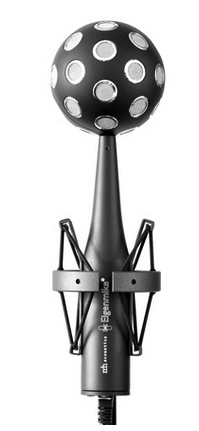
\includegraphics[width=\textwidth]{01_introduction/images/eigenmike_bw.png}
        \caption{Eigenmike}
        \label{fig:01_Introduction:Eigenmike}
    \end{subfigure}
    \hfill
    \begin{subfigure}[b]{0.3\textwidth}
        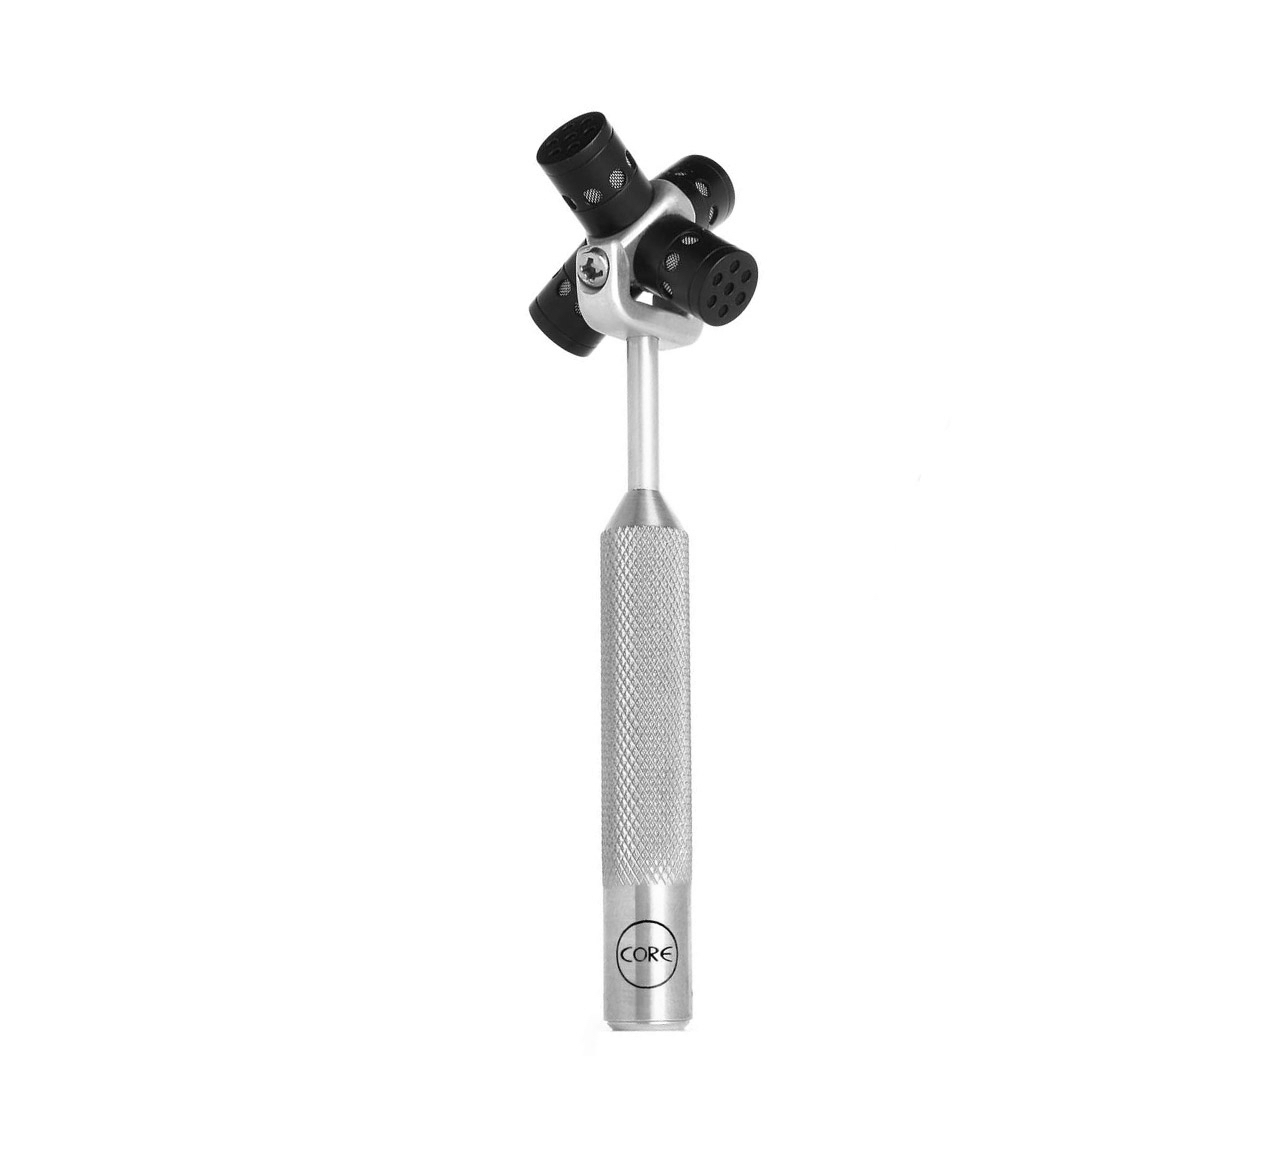
\includegraphics[width=\textwidth,trim={12cm 2cm 12cm 2cm},clip]{01_introduction/images/tetramic_bw.jpg}
        \caption{TetraMic}
        \label{fig:01_Introduction:TetraMic}
    \end{subfigure}
    \hfill
    \begin{subfigure}[b]{0.3\textwidth}
        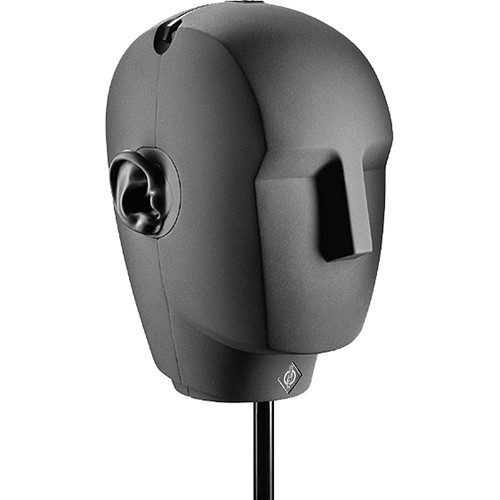
\includegraphics[width=\textwidth,trim={3cm 0 3cm 0},clip]{01_introduction/images/ku100_bw.jpg}
        \caption{KU-100}
        \label{fig:01_Introduction:KU100}
    \end{subfigure}
    \caption[Images of commercially-available spatial audio recording devices.]{
    Images of commercially-available spatial audio recording devices.
    The devices shown are
    the em32 Eigenmike by mh acoustics \citep{EigenmikeURL}, which captures HOA signals;
    the TetraMic by Core Sound \citep{TetraMicURL}, which captures FOA signals; and
    the KU-100 dummy head by Neumann \citep{NeumannKU100URL}, which captures binaural signals.
    }
\end{figure}

% for comparison, binaural has problems
For comparison, traditional binaural recordings (such as those made with a binaural dummy head, an example of which is shown in \figref{fig:01_Introduction:KU100}, or with a pair of small, in-ear microphones placed at the entrances of a human's ear canals) can provide a listener with an accurate spatial perception of a 3D sound field, but are inherently limited in two ways:
\begin{enumerate}
    \item the perspective experienced by the listener during playback is restricted to the vantage point of the recording individual (or device) in the original sound field and
    \item the 3D localization cues (i.e., information used by the human auditory system to determine the origin of a sound) embedded in the recording are only ideally suited for playback to the recording individual, as the recording individual's unique morphology (i.e., that individual's head-related transfer function, or HRTF) has already filtered the incoming sound waves in a highly idiosyncratic and direction-dependent manner.
\end{enumerate}
Examples of such localization cues include the \textit{interaural time difference}, i.e., the signal's time-of-arrival delay between the listener's ears; the \textit{interaural level difference}, i.e., the relative signal amplitudes between the listener's ears; and \textit{spectral cues}, which describe any spectral features added to the incoming sound that originate through interactions with the listener's morphology, e.g., pinnae (outer ears), head, and torso.
For a more thorough review of the fundamentals of sound localization, the interested reader is referred to the works of \citet[chapter 2]{Blauert1997} and \citet[section 1.4]{Xie2013}.

%% multi-binaural solves the rotation problem, but not the individualization problem
A partial solution to the former issue has been developed, known as ``motion-tracked binaural,'' in which multiple binaural signals are recorded (for example, by a roughly head-sized sphere with $\sim8$ microphones spaced around the horizontal-plane circumference) and, during playback, the listener's head rotation is measured and used to select (or compute via interpolation) the appropriate pair of signals \citep{Algazi2004}.
Measuring the listener's head movements is relatively straightforward using commercially-available head-tracking solutions%
\footnote{See, for example, the NaturalPoint TrackIR device (infrared) \citep{TrackIRURL}, the Polhemus Fastrak system (electromagnetic) \citep{PolhemusURL}, and the Visage Face Tracking software (facial recognition) \citep{VisageURL}.} 
and recently, commercial recording devices have been produced which include multiple sets of pinnae in order to produce more realistic binaural signals than those captured by a simple sphere.%
\footnote{See, for example, the 3Dio Omni Binaural Microphone \citep{3DioOmniBinauralURL} and the Hear360 8ball \citep{Hear3608ballURL}.}
This approach, however, can only account for azimuthal (yaw) head rotations; it cannot perform other head rotations (i.e., pitch or roll) or translations of the listener.
Additionally, unless the recording device is physically modified prior to recording to match the listener's particular HRTFs, these solutions fail to address the latter issue of individualization.

%% HOA-to-binaural solves individualization problem; requires HRTFs which are an active area of research
With an ambisonics recording, however, this latter issue can be resolved by post-processing the recorded signals with an individual's particular HRTFs, in a process known as \textit{binaural decoding} (or binaural rendering) of ambisonics.
When played back over headphones,%
\footnote{Alternatively, accurate binaural reproduction can be achieved using appropriately crosstalk-cancelled stereo loudspeaker systems \citep{Choueiri2017a}.}
the listener receives binaural signals that are (ideally) perceptually indistinguishable from those that would have been captured had the listener been physically present in the recorded sound field.
In principle, this approach can accurately produce the necessary 3D localization cues for any listener, although doing so requires accurately measured (or modeled) HRTFs for each listener, which are not trivial to acquire.
Indeed, the acquisition of accurate HRTFs, either through acoustical measurements or computational models, is its own vast and active area of research \citep{Nicol2010,Xie2013}.
Nevertheless, as such HRTF acquisition methods improve, binaural decoding of ambisonics will become ever more practical and accurate.

%% HOA-to-binaural easily performs listener rotation, but translation is more difficult
Existing binaural decoding techniques (several of which are reviewed in \secref{sec:02_Acoustical_Theory:Binaural_Rendering}) have primarily been developed only to place the listener at the position of the recording array \citep{McKeagMcGrath1996,Noisternig2003a,Duraiswami2005a,BergeBarrett2010b,Bernschutz2014} and consequently can only account for listener rotations.
Rotation of the listener (or, equivalently, of the sound field) in ambisonics is straightforward and has been well-established in the literature \citep{GumerovDuraiswami2005,Zotter2009PhD}, so we will not discuss it in detail; briefly, it involves the application of rotation matrices to change coordinates and a frequency-independent mixing of the ambisonics signals (formulae for some such rotation matrices are reproduced here in \secref{sec:A1_Navigation_Filters:Rotation_Matrices}).
In practice, these rotation matrices can be computed and applied in real-time based on the measured orientation of the listener's head.
Translations of the listener can also be performed in real-time based on either the measured position of the listener (e.g., from a head-tracking device) or some other user input, such as from a video game controller.
Methods to translate the listener, however, entail more complex processing and are not as well-established, nor have the penalties incurred by such processing been fully characterized.

%% translation is limited by theory and results in coloration & localization errors, but higher orders are better
Translation of the listener is made difficult by a well-known limitation of the ambisonics framework: that a finite-order expansion of a sound field yields only an approximation to that sound field, the accuracy of which decreases with increasing frequency and distance from the expansion center \citep{Poletti2005,WardAbhayapala2001}.
In particular, a well-established rule of thumb states that a sound field is accurately represented%
\footnote{Specifically, \citet{WardAbhayapala2001} show that obeying the inequality given in \eqnref{eq:01_Introduction:kr_Inequality} yields a \textit{reconstruction error} (i.e., the discrepancy between the exact pressure field and its order-limited approximation) of at most 4\%, which the authors claim ``should be sufficient for most practical applications.''}
by an $L^\textrm{th}$-order expansion up to a distance $r$ provided that
\begin{equation}\label{eq:01_Introduction:kr_Inequality}
kr \leq L,
\end{equation}
where $k$ is the angular wavenumber \citep[Eq.~(17)]{WardAbhayapala2001}
(cf.~\citet[Eq.~(28)]{Poletti2005} and \citet[p.~289]{Nicol2017}).
As a consequence, existing extrapolation-based navigational methods (hereafter referred to as \textit{extrapolation} methods,%
\footnote{In this thesis, we distinguish between two categories of navigational methods: \textit{extrapolation} methods, which employ only a single ambisonics microphone, and \textit{interpolation} methods, which employ an array of ambisonics microphones distributed throughout the sound field (or, equivalently, take samples at multiple discrete positions throughout a synthetic sound field).}
several of which are reviewed in \secref{sec:03_Navigation_Techniques:Extrapolation_Methods}) have been shown to introduce spectral coloration (i.e., audible changes in the spectral content of a signal) \citep{KuntzRabenstein2007,HahnSpors2015b} and localization errors (i.e., errors in the perceived direction of a sound relative to the listener) \citep{Winter2014,TylkaChoueiri2015} as the listener navigates farther away from the expansion center.%
\footnote{Similar results were found by \citet{WaltherFaller2010}, although their aim was not to navigate the sound field, but instead to simulate a spaced-microphone recording using a single first-order ambisonics microphone.}
However, previous studies have also shown (and we will also show here in \chapref{chap:07_Characterization_Extrapolation}) that these penalties decrease as the expansion order of the recording increases \citep{Winter2014,TylkaChoueiri2015}.
Thus, since synthetic sound fields can be generated to arbitrarily high orders, and since microphone array technology is rapidly advancing, it may soon be practical to capture very high-order expansions of real sound fields, thereby increasing the viability of extrapolation methods.

%% near-field sources, however, require additional steps
Another more fundamental limitation of the ambisonics description of sound fields is that the region over which the spherical-harmonic expansion is \textit{valid} is restricted by the nearest sound source or scattering body to the expansion center, so near-field sources and obstacles pose a particularly limiting problem to virtual navigation (see \secref{sec:02_Acoustical_Theory:Helmholtz_Equation} for a review of the relevant acoustical theory).
Although many sound fields are free of extremely near-field sources and obstacles, many of interest are not, so additional steps must be taken to overcome this limitation.
For example, if the near-field sources in a sound field can be identified, localized, and isolated from the rest of the recording, then they can be processed and rendered separately, thereby enlarging the effective region of validity for navigation.

%% broadly discuss recent developments (and introduce categorizations)
In recent work, \textit{parametric} navigational methods%
\footnote{So-called \textit{parametric} navigational methods are those that depend on additional information (e.g., source positions) beyond the ambisonics input signals in order to perform the navigation.
That is, the particular processing carried out by these methods directly depends on some such parameter of the sound field.
For \textit{linear} methods, on the other hand, all relevant parameters (e.g., virtual loudspeaker positions) may be specified offline, so the processing carried out during playback is independent of any changes to the sound field.}
have been developed to overcome this restriction by leveraging additional information about the positions of sources \citep{TylkaChoueiri2016,Wakayama2017}.
Additionally, navigational methods that employ multiple ambisonics microphones (hereafter referred to as \textit{interpolation} methods, several of which are reviewed in \secref{sec:03_Navigation_Techniques:Interpolation_Methods}) enable navigation near to and around such near-field sources \citep{TylkaChoueiri2016,Thiergart2013,Zheng2013PhD} (as will be shown in \chapreftwo{chap:08_Proposed_Method}{chap:09_Thiergart_Comparison}), although published findings on this subject are limited.
Existing navigational methods are summarized in \tabref{tab:01_Introduction:Methods}.

\begin{sidewaystable}
\centering
\begin{tabular}{l|c|c|c|l}
\textbf{Method} & \textbf{Processing} & $P$ & $L_\textrm{in}$ & \textbf{Additional Inputs} \\\hline\hline
Virtual ambisonics \citep[section 3.1]{TylkaChoueiri2015} & Linear & 1 & $1+$ & \\\hline
Plane-wave translation \citep{SchultzSpors2013} & Linear & 1 & $1+$ & \\\hline
Ambisonics translation \citep{GumerovDuraiswami2005,MenziesAlAkaidi2007a,Zotter2009PhD} & Linear & 1 & $1+$ & \\\hline
Singular ambisonics translation \citep{Wakayama2017} & Parametric & 1 & $1+$ & Source position \\\hline
Distance-mapped sound field modeling \citep{Plinge2018} & Parametric & 1 & 1 & Distance map of environment \\\hline
Spherical equivalent source method \citep{FernandezGrande2016} & Linear & $1+$ & $1+$ &  \\\hline
Inverse ambisonics translation via plane-waves \citep{WangChen2018} & Linear & $1+$ & $1+$ &  \\\hline
Sparse plane-wave estimation and translation \citep{Emura2017} & Nonlinear & 2 & $1+$ &  \\\hline
Weighted-average interpolation \citep{Southern2009,MarietteKatz2009} & Linear & $2+$ & $1+$ &  \\\hline
Regularized inverse ambisonics interpolation \citep{Samarasinghe2014a,TylkaChoueiri2016,Ueno2018} & Linear & $2+$ & $1+$ &  \\\hline
Distance-biased linear interpolation \citep{Patricio2019} & Linear & $2+$ & $1+$ &  \\\hline
Dynamic time warping RIR interpolation \citep{Masterson2009,Kearney2009} & Nonlinear & $2+$ & $1+$ & Source positions \\\hline
Valid-only interpolation \citep{TylkaChoueiri2016} & Parametric & $2+$ & $1+$ & Source positions \\\hline
Time-frequency analysis and modeling \citep{Thiergart2013} & Parametric & $2+$ & 1 &  \\\hline
Collaborative blind-source separation \citep{Zheng2013PhD} & Parametric & $2+$ & 1 &  \\\hline
Perspective control ambisonics microphone array \citep{Bates2018} & Parametric & 4 & $1+$ & 
\end{tabular}
\caption[Summary of published navigational methods.]{
Summary of published navigational methods.
Here, $P$ denotes the number of ambisonics microphones used in the method and $L_\text{in}$ denotes the required ambisonics order of the microphone(s).}
\label{tab:01_Introduction:Methods}
\end{sidewaystable}

% Review previous work focusing on the remaining problems (questions or deficiencies) the present paper claims to contribute to solving
\section{Previous work and remaining problems}
% metrics problem - POMA paper, Ch. 5
As mentioned above, numerous methods for virtual navigation have been developed, many of which have been shown to introduce localization errors \citep{Winter2014,TylkaChoueiri2015,TylkaChoueiri2016} and/or spectral coloration \citep{HahnSpors2015b,TylkaChoueiri2016}.
Although subjective testing is the most direct means of evaluating and comparing navigational methods in terms of these perceptual attributes, such tests are often lengthy and costly, which motivates the use of objective metrics that enable quick assessments of navigational methods.
Existing perceptually-motivated objective metrics often rely on computational models of the human auditory system (so-called ``binaural models'') in order to predict some aspect of the perception of a sound (e.g., perceived source position or spectral content) by a ``typical'' human listener.
Such metrics necessarily conflate the effects of the navigational method with those of the adopted ambisonics-to-binaural rendering approach.
On the other hand, purely signal- or physics-based metrics may circumvent this issue by evaluating the signals prior to rendering to binaural, but they are not necessarily perceptually relevant, in that their predictions may not correspond with subjective listening test responses.
Consequently, suitable (i.e., perceptually relevant and non-binaural) objective metrics for at least coloration and localization are needed in order to both compare existing navigational methods and develop future ones.

% simulation framework - Ch. 6 --> 10
Additionally, each study that has previously attempted to quantify the incurred perceptual penalties often only examined a single navigational method, considered a limited range of conditions (e.g., sound field geometry, input ambisonics order, etc.), and employed a unique set of objective metrics, thus making comparisons across studies essentially impossible.
In order to draw meaningful comparisons between competing navigational methods, a consistent and comprehensive set of tests should be designed and conducted for all existing and future methods.

% comparison of extrapolation methods and quantification of validity penalties - Ch. 7
With the exception of the plane-wave translation method of \citet{SchultzSpors2013} (which we review in \secref{sec:03_Navigation_Techniques:PW_Technique}), most existing extrapolation methods have not been evaluated in terms of perceptual attributes (i.e., coloration and localization).
In particular, any errors related to the region of validity restriction (which all linear extrapolation methods are prone to violate if the listener navigates beyond a near-field source) have not been well-established in the literature.
Additionally, the penalties incurred by different methods have only been directly compared over a limited range of conditions \citep{TylkaChoueiri2015}, making it difficult to choose the appropriate method for a particular application.
Consequently, the performance of existing extrapolation methods should be characterized and compared, and the errors incurred by violating the region of validity restriction should be quantified.

% quantification of validity penalties for interpolation methods - AES 2016 AVAR Paper, Ch. 8
Parametric and interpolation methods may provide adequate solutions to the region of validity restriction, but this issue has not been explored much in the literature.
The simplest existing interpolation method entails a weighted average of the ambisonics signals from different microphones \citep{Southern2009} and (as we will show in \secref{sec:08_Proposed_Method:Fundamental_Problems}) is consequently prone to comb-filtering-like effects and skewed localization due to the precedence effect.
An alternative, least-squares interpolation method may mitigate these issues \citep{Samarasinghe2014a}, but remains prone to violating the region of validity restriction if the sound field contains any near-field sources.
Consequently, in a recent publication, we proposed a parametric interpolation method which ensures that this restriction is not violated \citep{TylkaChoueiri2016}.
Additionally, a recently-proposed parametric extrapolation method circumvents this restriction using \textit{a priori} information of the source positions \citep{Wakayama2017}, and other parametric methods have been developed that construct a navigable model of the incident sound field via a time-frequency analysis \citep{Thiergart2013,Zheng2013PhD,Plinge2018}, and should consequently be immune to this restriction.
However, the performance of these methods has not been fully characterized in terms of perceptual criteria and, in particular, the penalties incurred by violations of the region of validity restriction have not been established.

% comparison of parametric methods - Ch. 9
Finally, the suitability of such methods for different applications has not been established.
For example, while recently-developed parametric methods may yield more accurate localization than linear methods, even in the presence of near-field sources, they have been shown to introduce minor degradations of sound quality \citep[section 5.3]{Zheng2013PhD} and they may not be suitable for dense or highly-reverberant environments \citep[section II]{Thiergart2013}.
Consequently, based on a broad performance characterization of existing parametric interpolation methods, recommendations should be made regarding the suitability of each method to various applications.

%%%% Objectives and Approach %%%%
% A statement of the paper's main question(s) and goal(s), followed by a succinct description of the general method and approach to be described in the paper
\section{Objectives and approach}
It is the overall objective of this thesis to investigate the limitations of, and penalties incurred by, various methods for virtual sound field navigation.
Of particular interest are those penalties relating to a violation of the region of validity restriction.
To these ends, we first develop, and subsequently validate through subjective listening experiments, perceptually-relevant objective metrics for perceived spectral coloration and source localization errors introduced by navigational methods. % Ch. 5
We then design, and later experimentally validate, a numerical simulation framework based on simple incident sound fields, which enables a consistent and comprehensive performance characterization (in terms of a suite of perceptually-relevant objective metrics) across navigational methods. % Ch. 6
To validate these simulations, we perform a set of acoustical measurements taken over a subset of the simulated conditions and determine the magnitudes of any discrepancies in the resulting values of each objective metric. % Ch. 10

Next, we characterize the performance of existing extrapolation methods in order to identify regimes in which each method performs well and to provide insight into the types and severities of incurred penalties under a range of conditions. % Ch. 7
We then revise our previously-proposed parametric interpolation method \citep{TylkaChoueiri2016} in order to mitigate its induced spectral coloration and to characterize and compare the performance of this method and that of a benchmark linear method. % Ch. 8
Similarly, we characterize and compare the performance of an existing parametric time-frequency interpolation method and our revised method. % Ch. 9
From each of these characterizations, we seek broader insights into the nature of the penalties incurred by violating the region of validity restriction and identify considerations regarding the suitability of each method to various applications. % Ch. 11

% A brief section by section description of the structure of the paper
\section{Thesis overview}
The remainder of the present thesis is organized as follows.
The next three chapters consist largely of review material:
\begin{itemize}
\item in \chapref{chap:02_Acoustical_Theory}, we review relevant concepts from acoustics and ambisonics theory;
\item in \chapref{chap:03_Navigation_Techniques}, we review several existing navigational methods; and
\item in \chapref{chap:04_Auditory_Models}, we review existing objective metrics and auditory models.
\end{itemize}
Then, in \chapref{chap:05_Proposed_Models}, we propose auditory models for spectral coloration and localization, describe experiments for their subjective validation, and present corresponding results.
Next, in \chapref{chap:06_Simulation_Framework}, we present the numerical simulation framework employed in subsequent chapters to characterize and compare navigational methods.
The following three chapters consist largely of performance characterizations:
\begin{itemize}
\item in \chapref{chap:07_Characterization_Extrapolation}, we characterize and compare the performance of two existing linear extrapolation methods, and identify penalties incurred by violating the region of validity restriction;
\item in \chapref{chap:08_Proposed_Method}, we revise our previously-proposed parametric interpolation method, and characterize and compare its performance and that of a benchmark linear method; and
\item in \chapref{chap:09_Thiergart_Comparison}, we characterize and compare the performance of an existing parametric interpolation method and our proposed method, and identify suitable domains for the practical application of each method.
\end{itemize}
We then present, in \chapref{chap:10_Experimental_Validation}, an experimental validation of the numerical simulation framework described in \chapref{chap:06_Simulation_Framework}.
Finally, in \chapref{chap:11_Conclusions}, we summarize the major findings from this work; synthesize these findings into a) broader insights regarding the penalties incurred by violating the region of validity restriction and b) guidelines regarding the practical application of each method; and propose avenues for future research.

\section{Relevant prior publications}
Many of the chapters and appendices in this thesis are largely based on the following prior publications by the present author:
\begin{itemize}
\item \chapref{chap:05_Proposed_Models} -- \citet{TylkaChoueiri2017a}
\item \chapref{chap:07_Characterization_Extrapolation} -- \citet{TylkaChoueiri2015} and \citet{TylkaChoueiri2019c} (submitted)
\item \chapref{chap:08_Proposed_Method} -- \citet{TylkaChoueiri2016} and \citet{TylkaChoueiri2019b} (submitted)
\item \chapref{chap:09_Thiergart_Comparison} -- \citet{TylkaChoueiri2019d} (submitted)
\item \chapref{chap:10_Experimental_Validation} -- \citet[section 6]{TylkaChoueiri2019b} (submitted)
\item \apxref{chap:A1_Navigation_Filters} -- \citet{TylkaChoueiri2019a}
\item \apxref{chap:A2_SABRE_Toolkit} -- \citet{TylkaChoueiri2017b}
\item \apxref{chap:A3_Smoothing_Weights} -- \citet*{Tylka2017}
	\begin{itemize}
	\item I performed all of the analysis presented in this publication, although Prof.~Boren conducted some of the initial investigations into the issue, and together we had several fruitful discussions to better identify the problem and which led to the development of the presented smoothing method.
	\end{itemize}
\item \apxref{chap:A4_HRTF_Measurements} -- \citet*{Sridhar2017}
	\begin{itemize}
	\item Mr.~Sridhar was responsible for all of the work on morphological scans described in this publication, but this work is omitted in this appendix.
	Mr.~Sridhar and I contributed equally to the construction of the experimental hardware used to measured the HRTFs, and to the development of the data acquisition and analysis software.
	\end{itemize}
\item \apxref{chap:A5_Impulse_Response} -- \citet*{Tylka2014}
	\begin{itemize}
	\item Mr.~Sridhar and I contributed equally to the development of the presented iterative method and to the experiments and analyses presented in this publication, although only the introductory and background sections, which I have significantly revised, are reproduced in this appendix.
	Prof.~Boren conducted some of the initial investigations into the issue and provided guidance towards the overall direction of the research.
	\end{itemize}
\end{itemize}
Except where noted otherwise, all of the work presented in the papers listed above is my own, with Prof.~Choueiri serving in an advisory capacity and lending guidance towards the overall direction of the research.
\chapter{Review of acoustical and ambisonic theory}\label{chap:02_Acoustical_Theory}
In this chapter, we review relevant acoustical and ambisonic theory which will be employed throughout this thesis.
First, in \secrefthru{sec:02_Acoustical_Theory:Coordinate_System}{sec:02_Acoustical_Theory:Helmholtz_Equation}, we review the spherical Fourier-Bessel series solution to the free-field Helmholtz equation in three dimensions, which provides a frequency-domain representation of any sound pressure field in spherical coordinates.
These solutions lay the mathematical foundation for ambisonics, which we adopt to formulate the problem of virtual navigation in general, as described in \secref{sec:03_Navigation_Techniques:Problem_Formulation}, as well as to describe the implementation of each existing navigational method reviewed in \secreftwo{sec:03_Navigation_Techniques:Extrapolation_Methods}{sec:03_Navigation_Techniques:Interpolation_Methods}.

Next, in \secref{sec:02_Acoustical_Theory:Ambisonics_Encoding}, we review the so-called \textit{ambisonic encoding} equations for synthesizing ambisonics signals for point-sources and plane-waves.
These encoding equations are employed in order to simulate simple incident sound fields, as described in \chapref{chap:06_Simulation_Framework}.
These simulations are later used to comprehensively characterize the performance of various navigational methods, as described in \chaprefthru{chap:07_Characterization_Extrapolation}{chap:09_Thiergart_Comparison}.

In \secref{sec:02_Acoustical_Theory:Plane-Wave_Expansion}, we provide equations for converting between spherical-harmonic (i.e., ambisonic) and plane-wave representations of a sound field, a process which is used in the plane-wave translation method reviewed in \secref{sec:03_Navigation_Techniques:PW_Technique}.
The conversion from ambisonics to plane-wave signals is also used in the plane-wave-based ambisonics-to-binaural rendering approach described in \secref{sec:02_Acoustical_Theory:PW_Quadrature_Binaural}, as well as in the localization model proposed in \secref{sec:05_Proposed_Models:Localization_Model}.
Next, in \secref{sec:02_Acoustical_Theory:Ambisonics_Translation}, we review the spherical Fourier-Bessel translation coefficients, which are needed for the ambisonics translation method reviewed in \secref{sec:03_Navigation_Techniques:SR_Technique}.

Finally, in \secref{sec:02_Acoustical_Theory:Binaural_Rendering}, we review three linear ambisonics-to-binaural rendering approaches, one of which is employed in the listening experiments presented in \chapref{chap:05_Proposed_Models}, and all three of which have been implemented in the MATLAB toolkit described in \apxref{chap:A2_SABRE_Toolkit}.

\section{Coordinate system}\label{sec:02_Acoustical_Theory:Coordinate_System}
As is common in ambisonics, we adopt Cartesian and spherical coordinate systems in which, for a listener positioned at the origin, the $+x$-axis points forward, the $+y$-axis points to the left, and the $+z$-axis points upward.
The point $(x,y,z)$ in Cartesian coordinates is given in spherical coordinates by
\begin{equation}\label{eq:02_Acoustical_Theory:Spherical_Coordinates}
\begin{aligned}
    r &= \sqrt{x^2 + y^2 + z^2},\\
    \theta &= \arcsin \frac{z}{r},\\ % = \arcsin \mu
    \phi &= \arctan \frac{y}{x}.
\end{aligned}
\end{equation}
From this definition we see that $r$ is the (nonnegative) radial distance from the origin, $\theta \in [-\pi/2, \pi/2]$ is the elevation angle above the horizontal ($x$-$y$) plane, and $\phi \in [0, 2\pi)$ is the azimuthal angle around the vertical ($z$) axis, with $(\theta,\phi) = (0,0)$ corresponding to the $+x$ direction and $(0,\pi/2)$ to the $+y$ direction.
These variables are defined graphically in~\figref{fig:02_Acoustical_Theory:Coordinate_System}.
Conversion back to Cartesian coordinates is given by
\begin{equation}\label{eq:02_Acoustical_Theory:Cartesian_Coordinates}
\begin{aligned}
    x &= r \cos \theta \cos \phi,\\
    y &= r \cos \theta \sin \phi,\\
    z &= r \sin \theta.
\end{aligned}
\end{equation}
For a position vector $\vec{r} = (x,y,z)$, we denote the corresponding unit vector by $\hat{r} \equiv \vec{r}/r$.

\tdplotsetmaincoords{60}{120}

\pgfmathsetmacro{\rvec}{.8}
\pgfmathsetmacro{\thetavec}{30}
\pgfmathsetmacro{\phivec}{60}

\begin{figure}[t]
\centering
\begin{tikzpicture}[scale=5,tdplot_main_coords]

    \coordinate (O) at (0,0,0);
    \draw[thick,->] (0,0,0) -- (1,0,0) node[anchor=north east]{$x$};
    \draw[thick,->] (0,0,0) -- (0,1,0) node[anchor=north west]{$y$};
    \draw[thick,->] (0,0,0) -- (0,0,1) node[anchor=south]{$z$};
    \tdplotsetcoord{P}{\rvec}{\thetavec}{\phivec}
    \draw[thick,->] (O) -- (P) node[above right] {$\vec{r}$};
    \draw[dashed] (O) -- (Pxy);
    \draw[dashed] (P) -- (Pxy);
    \tdplotdrawarc{(O)}{0.2}{0}{\phivec}{anchor=north}{$\phi$}
    \tdplotsetthetaplanecoords{\phivec}
    \tdplotdrawarc[tdplot_rotated_coords]{(0,0,0)}{0.2}{90}{\thetavec}{anchor=south west}{$\theta$}

\end{tikzpicture}
\caption{Coordinate system.}\label{fig:02_Acoustical_Theory:Coordinate_System}
\end{figure}

%% Short version for papers
%As is common in ambisonics, we adopt Cartesian and spherical coordinate systems in which, for a listener positioned at the origin, the $+x$-axis points forward, the $+y$-axis points to the left, and the $+z$-axis points upward.
%Correspondingly, $r$ is the (nonnegative) radial distance from the origin, $\theta \in [-\pi/2, \pi/2]$ is the elevation angle above the horizontal ($x$-$y$) plane, and $\phi \in [0, 2\pi)$ is the azimuthal angle around the vertical ($z$) axis, with $(\theta,\phi) = (0,0)$ corresponding to the $+x$ direction and $(0,\pi/2)$ to the $+y$ direction.
%For a position vector $\vec{r} = (x,y,z)$, we denote the corresponding unit vector by $\hat{r} \equiv \vec{r}/r$.

\section{Definitions and conventions}\label{sec:02_Acoustical_Theory:Definitions}
We define the Fourier transform for acoustic signals and its corresponding inverse transform as
\begin{equation}\label{eq:02_Acoustical_Theory:Fourier_Transform}
\begin{aligned}
H(\omega) = \mathcal{F}\left[ h(t) \right] (\omega) &= \frac{1}{2 \pi} \int_{-\infty}^{\infty} h(t) e^{i \omega t}dt,\\
h(t) = \mathcal{F}^{-1}\left[ H(\omega) \right] (t) &= \int_{-\infty}^{\infty} H(\omega) e^{-i \omega t}d\omega,
\end{aligned}
\end{equation}
where $\omega$ is the angular frequency in rad/s, which is related to the temporal frequency, $f$, given in Hz, by $\omega = 2 \pi f$.
We also define the convolution operator `$\ast$' by
\begin{equation}
(h \ast g)(t) = \int_{-\infty}^{\infty} h(\tau) g(t-\tau) d\tau,
\end{equation}
which, by the convolution theorem for the Fourier transform, implies
\begin{equation}
\begin{gathered}
\mathcal{F}\left[ (h \ast g)(t) \right] (\omega) = \mathcal{F}\left[ h(t) \right] (\omega) \cdot \mathcal{F}\left[ g(t) \right] (\omega) = H(\omega) G(\omega),\\
(h \ast g)(t) = \mathcal{F}^{-1}\left[ \mathcal{F}\left[ h(t) \right] (\omega) \cdot \mathcal{F}\left[ g(t) \right] (\omega) \right] (t) = \mathcal{F}^{-1}\left[ H(\omega) G(\omega) \right] (t),
\end{gathered}
\end{equation}
where $G(\omega) = \mathcal{F}\left[ g(t) \right] (\omega)$.

Here, we use real-valued spherical harmonics, such that the spherical harmonic of degree%
\footnote{Note that ambisonics literature has long interchanged the use of the terms ``degree'' and ``order'' compared to traditional mathematical definitions of the spherical harmonics, which originate from the solutions to Laplace's equation in spherical coordinates.
Hence, the ambisonics \textit{order} actually corresponds to the mathematical \textit{degree} of the spherical harmonic.}
$l$ and order $m$ is given by~\citet[section~2.2]{Zotter2009PhD}
\begin{equation}\label{eq:02_Acoustical_Theory:Spherical_Harmonic}
Y_l^m(\theta,\phi) = N_l^{|m|} P_l^{|m|} (\sin \theta) \times
    \begin{cases}
	\cos m \phi & \textrm{for } m \geq 0,\\
	\sin |m| \phi & \textrm{for } m < 0,
    \end{cases}
\end{equation}
where $P_l^m$ is the associated Legendre polynomial of degree $l$ and order $m$, as defined in the MATLAB \texttt{legendre} function\citefooturl{MATLABlegendreURL} by
\begin{equation}
P_l^m(x) = (-1)^m (1 - x^2)^{m/2} \frac{d^m}{dx^m} P_l(x), \quad
\textrm{with} \quad
P_l(x) = \frac{1}{2^l l!} \left[ \frac{d^l}{dx^l}(x^2 - 1)^l \right],
\end{equation}
and $N_l^m$ is a normalization term which, for the orthonormal (N3D) spherical harmonics with Condon-Shortley phase,%
\footnote{Note that including Condon-Shortley phase in the normalization term cancels it in the associated Legendre term.} is given by
\begin{equation}\label{eq:02_Acoustical_Theory:Spherical_Harmonic_N3D_Normalization}
N_l^m = (-1)^m \sqrt{\frac{(2l+1)(2 - \delta_m)}{4 \pi} \frac{(l-m)!}{(l+m)!}},
\end{equation}
where $\delta_m$ is the single-argument Kronecker delta.

We define an inner product on the unit sphere by
\begin{equation}
\left< h, g \right> \equiv \int_{\phi=0}^{2 \pi} \int_{\theta=-\frac{\pi}{2}}^{\frac{\pi}{2}} h(\theta,\phi) \overline{g(\theta,\phi)} \cos \theta d\theta d\phi,
\end{equation}
where $\overline{g}$ denotes the complex conjugate of $g$.
Therefore, the inner product of any two N3D-normalized spherical harmonic functions is given by
\begin{equation}
\left< Y_l^m, Y_{l'}^{m'} \right> = \delta_{l,l'} \delta_{m,m'},
\end{equation}
where $\delta_{m,m'}$ is the Kronecker delta (with two arguments),
and the squared norm of any spherical harmonic function is given by
\begin{equation}
\|Y_l^m\|^2 \equiv \left< Y_l^m, Y_l^m \right> = 1.
\end{equation} % Follows from inner product
Consequently, we see that the N3D spherical harmonics form an orthonormal basis on the unit sphere.

A commonly-used alternative is the Schmidt seminormalized (SN3D) spherical harmonic normalization convention (again with Condon-Shortley phase), given by \citep{Nachbar2011}
\begin{equation}\label{eq:02_Acoustical_Theory:Spherical_Harmonic_SN3D_Normalization}
N_l^m = (-1)^m \sqrt{\frac{2 - \delta_m}{4 \pi} \frac{(l-m)!}{(l+m)!}}.
\end{equation}
With the same choice of inner product, the inner product of any two spherical harmonic functions is given by
\begin{equation}
\left< Y_l^m, Y_{l'}^{m'} \right> = \frac{\delta_{l,l'} \delta_{m,m'}}{2l+1}
\end{equation}
and the squared norm of any spherical harmonic function is given by
\begin{equation}
\|Y_l^m\|^2 = \frac{1}{2l+1}.
\end{equation} % Follows from inner product
Consequently, we note that the SN3D spherical harmonics are \textit{not} orthonormal on the unit sphere, but they do yield an orthogonal basis.

We also adopt the ambisonics channel numbering (ACN) convention~\citep{Nachbar2011} such that for a spherical harmonic function of degree $l \in [0,\infty)$ and order $m \in [-l,l]$, the ACN index $n$ is given by
\begin{equation}\label{eq:02_Acoustical_Theory:AmbOrder_To_ACN}
n = l (l + 1) + m
\end{equation}
and we denote the spherical harmonic function by $Y_n \equiv Y_l^m$.
Correspondingly, for ACN index $n$, the spherical harmonic degree and order are given by
\begin{equation}\label{eq:02_Acoustical_Theory:ACN_To_AmbOrder}
\begin{aligned}
l &= \left\lfloor \sqrt{n} \right\rfloor,\\
m &= n - l (l + 1),
\end{aligned}
\end{equation}
where $\lfloor \cdot \rfloor$ denotes rounding down to the nearest integer (i.e., the ``floor'' function).

Alternative ordering and normalization schemes, such as Furse-Malham (``FuMa'') and ``MaxN'', are discussed by \citet[and references therein]{Carpentier2017}.

\section{Helmholtz equation and region of validity}\label{sec:02_Acoustical_Theory:Helmholtz_Equation}
We define the \textit{acoustic potential field} $\psi$ as the Fourier transform of the acoustic pressure field, such that, in the \textit{free-field} (i.e., in a region free of sources and scattering bodies), the acoustic potential field satisfies the homogeneous Helmholtz equation,
\begin{equation}\label{eq:02_Acoustical_Theory:Helmholtz_Equation}
\left( \nabla^2 + k^2 \right) \psi(k,\vec{r}) = 0,
\end{equation}
where $\nabla^2$ is the Laplace operator, $k = \omega / c$ is the angular wavenumber, and $c \approx 343$~m/s is the speed of sound.

Depending on our region of interest, we may impose different boundary conditions on the problem in order to ensure that our solution for the acoustic potential field is physically possible.
For example, for an exterior (free-field) region of interest, all sources and obstacles must exist within a spherical region centered on the origin and of some finite radius, $R$.
Consequently, the solution must satisfy the Sommerfeld radiation condition \citep[section 2.1.1]{Zotter2009PhD}, which can be written as
\begin{equation}
\lim_{r\to\infty} \left[ r \left( \frac{\partial}{\partial r} - i k \right) \psi (k,\vec{r}) \right] = 0.
\end{equation}
Although multiple physical interpretations of this condition exist (cf.~\citet[appendix A]{Zotter2009PhD}, \citet[section 4-5]{Pierce1994}), essentially it states that power must only be radiating away from sources located near the origin, rather than arriving from infinity and being destroyed \citep{WikiSommerfeldURL}.
In this case, we must choose singular, radiating basis solutions to the Helmholtz equation, which are given by $h_l(kr) Y_n(\hat{r})$, where $h_l$ is the (outgoing) spherical Hankel function of the first kind and of order $l$, and $Y_n$ is the spherical harmonic for ACN index $n$ \citep[section 6.7]{Williams1999}.
The interested reader is referred to the works of \citet{Zotter2009PhD,Williams1999} for more detailed discussions of such exterior problems.

For an interior region of interest, where all sources exist beyond some finite radius $R$ away from the origin, we require that the solution be finite in magnitude everywhere inside that region, i.e., $|\psi| < \infty,~\forall r < R$.
In this case, we must choose regular (i.e., not singular) basis solutions to the Helmholtz equation, which are given by $j_l(kr) Y_n(\hat{r})$, where $j_l$ is the spherical Bessel function of order $l$ \citep[section 6.8]{Williams1999}.
%These solutions are only valid under free-field conditions, and can be used to describe the acoustic potential in an interior region, that is, for $r < R$, where $R$ is a finite distance .
%So that the region remains source- and obstacle-free, $R$ is typically taken to be the distance of the nearest source or scattering body to the origin.
This spherical interior region where $r < R$ is the so-called \textit{region of validity}, which is illustrated in \figref{fig:02_Acoustical_Theory:Region_of_Validity}.

% Diagram of source/mic positions
\begin{figure}[t]
\centering
  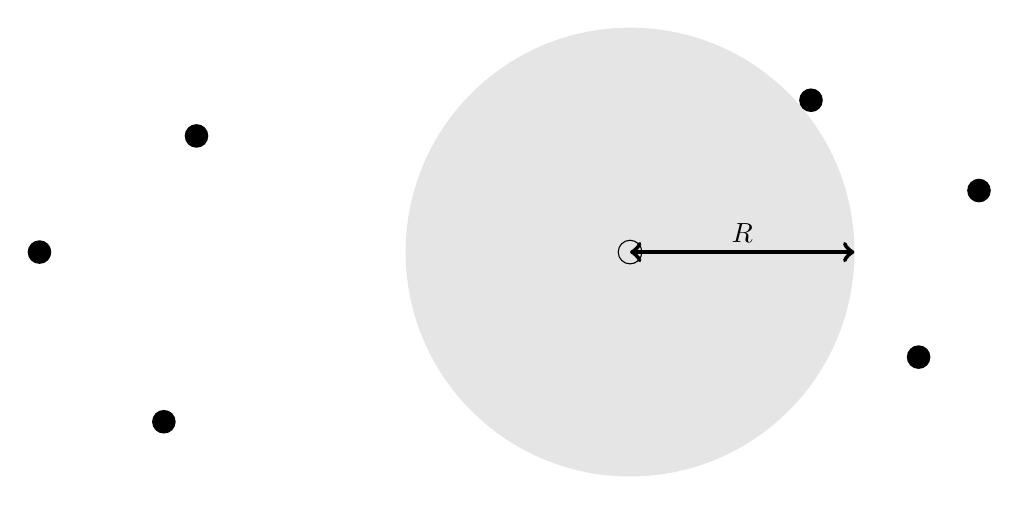
\begin{tikzpicture}[scale=3]
% Parameters
\def\radius{1};
\def\validR{0.95};
\def\sourceR{1-\validR}

\pgfmathsetmacro\evalX{cos(140)*\radius}
\pgfmathsetmacro\evalY{sin(140)*\radius}

\pgfmathsetmacro\sourceXa{cos(-20)*1.3*\radius}
\pgfmathsetmacro\sourceYa{sin(-20)*1.3*\radius}

\pgfmathsetmacro\sourceXb{cos(10)*1.5*\radius}
\pgfmathsetmacro\sourceYb{sin(10)*1.5*\radius}

\pgfmathsetmacro\sourceXc{cos(200)*2.1*\radius}
\pgfmathsetmacro\sourceYc{sin(200)*2.1*\radius}

\pgfmathsetmacro\sourceXd{cos(180)*2.5*\radius}
\pgfmathsetmacro\sourceYd{sin(180)*2.5*\radius}

\pgfmathsetmacro\sourceXe{cos(165)*1.9*\radius}
\pgfmathsetmacro\sourceYe{sin(165)*1.9*\radius}

\pgfmathsetmacro\sourceXf{cos(40)*\radius}
\pgfmathsetmacro\sourceYf{sin(40)*\radius}

\fill [color=black,opacity=0.1] (0,0) circle (\validR*\radius);

%\node at (0,0){$\times$};
\draw [color=black] (0,0) circle (\sourceR*\radius);
\draw[ultra thick,<->] (0,0) -- (\validR*\radius,0);
\node[above] at (0.5*\validR*\radius,0){$R$};

% Source positions
\fill [color=black] (\sourceXa,\sourceYa) circle (\sourceR*\radius);
\fill [color=black] (\sourceXb,\sourceYb) circle (\sourceR*\radius);
\fill [color=black] (\sourceXc,\sourceYc) circle (\sourceR*\radius);
\fill [color=black] (\sourceXd,\sourceYd) circle (\sourceR*\radius);
\fill [color=black] (\sourceXe,\sourceYe) circle (\sourceR*\radius);
\fill [color=black] (\sourceXf,\sourceYf) circle (\sourceR*\radius);
\end{tikzpicture}
  \caption[Diagram of the region of validity for an interior free-field region.]{
  Diagram of the region of validity for a free-field spherical Fourier-Bessel expansion.
  The empty circle indicates the expansion center,
  the filled circles indicate source positions,
  and the shaded disk indicates the region of validity.
  The radius of the region of validity is equal to $R$, the distance of the nearest source from the expansion center.}
  \label{fig:02_Acoustical_Theory:Region_of_Validity}
\end{figure}

Inside this region, any acoustic potential field can be written as an infinite sum of regular solutions, known as a spherical Fourier-Bessel series expansion, given by \citep[chapter 2]{GumerovDuraiswami2005}
\begin{equation}\label{eq:02_Acoustical_Theory:Infinite_Order_Expansion}
\psi(k,\vec{r}) = \sum_{n=0}^{\infty} 4\pi (-i)^l A_n(k) j_l(kr) \frac{Y_n(\hat{r})}{\|Y_n\|^2},
\end{equation}
where $A_n$ are the corresponding (frequency-dependent) expansion coefficients and we have, without loss of generality, factored out $(-i)^l$ to ensure conjugate-symmetry in each $A_n$, making each ambisonics signal (i.e., the inverse Fourier transform of $A_n$) real-valued for a real pressure field.
Note that this expansion need not be taken about the origin, but instead can be taken about any arbitrary expansion center, in which case the region of validity refers to a spherical free-field region centered about that point.
In practice, this expansion is truncated to a finite order $L$ (i.e., $l \in [0,L]$), yielding $N = (L + 1)^2$ terms,
\begin{equation}\label{eq:02_Acoustical_Theory:Finite_Order_Expansion}
\psi(k,\vec{r}) = \sum_{n=0}^{N - 1} 4\pi (-i)^l A_n(k) j_l(kr) \frac{Y_n(\hat{r})}{\|Y_n\|^2}.
\end{equation}

\section{Ambisonics encoding equations}\label{sec:02_Acoustical_Theory:Ambisonics_Encoding}
For a point-source that generates an impulse at $t = t_0$ and is located at $\vec{s}_0$, the emitted pressure field (impulse response) is given by
\begin{equation}
p(t,\vec{r}) = \frac{2 \pi}{\left\| \vec{r} - \vec{s}_0 \right\|} \cdot \delta \left( (t-t_0) - \frac{\left\| \vec{r} - \vec{s}_0 \right\|}{c} \right),
\end{equation}
where $\|\cdot\|$ denotes the $\ell^2$ norm (Euclidean distance) of a vector.
Taking the Fourier transform yields the acoustic potential field (transfer function) of that point-source, given by \citep[Eq.~(6.73)]{Williams1999}
\begin{equation}\label{eq:02_Acoustical_Theory:PointSource}
\psi(k,\vec{r}) = \frac{e^{i k \left\| \vec{r} - \vec{s}_0 \right\|}}{\left\| \vec{r} - \vec{s}_0 \right\|} e^{i k c t_0} = i k \cdot h_0 (k \left\| \vec{r} - \vec{s}_0 \right\| ) \cdot e^{i k c t_0}.
\end{equation} % Confirmed in Mathematica
%where, in general, $h_l$ is the (outgoing) spherical Hankel function of the first kind and of order $l$.
The spherical Fourier-Bessel expansion of this expression (ignoring the time delay term) is given by~\citep[Eq.~(8.22)]{Williams1999}
\begin{align}
\frac{e^{i k \left\| \vec{r} - \vec{s}_0 \right\|}}{\left\| \vec{r} - \vec{s}_0 \right\|} &= 4 \pi i k \sum_{l=0}^{\infty} j_l(k r) h_l(k s_0) \sum_{m=-l}^{l} Y_l^m (\hat{s}_0) \frac{Y_l^m (\hat{r})}{\|Y_l^m\|^2} \\
	&= \sum_{n=0}^{\infty} \left[ i^{l+1} k h_l(k s_0) Y_n (\hat{s}_0) \right] 4 \pi (-i)^l j_l(k r) \frac{Y_n (\hat{r})}{\|Y_n\|^2},
\end{align} % Confirmed in MATLAB
where we have assumed $r < s_0$ in order for $\vec{r}$ to be within the region of validity.
Thus, the ambisonics encoding filters for this point source are given by
\begin{equation}\label{eq:02_Acoustical_Theory:PointSource_An}
A_n(k) = \underbrace{i^{l+1} k h_l(k s_0)}_{\text{distance coding}} \underbrace{Y_n (\hat{s}_0)}_{\text{panning}} \underbrace{ \vphantom{ Y_n (\hat{s}_0) } e^{i k c t_0}}_{\text{delay}}.
\end{equation}

%The ambisonics encoding filters for a point source located at $\vec{s}_0$ are given in the frequency domain by~\citep[Eq.~(10)]{Poletti2005}
%\begin{equation}\label{eq:02_Acoustical_Theory:PointSource_An}
%A_n(k) = i^{l+1} k h_l(k s_0) Y_n (\hat{s}_0),
%\end{equation}
%where $h_l$ is the (outgoing) spherical Hankel function of order $l$.

For a plane-wave source located in the direction $\hat{s}_0$ (and propagating in the direction $-\hat{s}_0$), the pressure field is given by
\begin{equation}
p(t,\vec{r}) = 2 \pi \cdot \delta \left( (t-t_0) + \frac{\hat{s}_0 \cdot \vec{r}}{c} \right),
\end{equation}
where now $t = t_0$ indicates the time at which the impulse reaches the origin ($r = 0$).
Taking the Fourier transform yields the acoustic potential field of this plane-wave, given by \citep[Eq.~(2.24), with $\vec{k} = -k\hat{s}_0$]{Williams1999}
\begin{equation}
\psi(k,\vec{r}) = e^{-i k \hat{s}_0 \cdot \vec{r}} e^{i k c t_0}.
\end{equation} % Confirmed in Mathematica
The spherical Fourier-Bessel expansion of this expression (ignoring the time delay term) is given by~\citep[Eq.~(6.175)]{Williams1999}
\begin{align}
e^{-i k \hat{s}_0 \cdot \vec{r}} &= 4 \pi \sum_{l=0}^{\infty} i^l j_l(k r) \sum_{m=-l}^{l} Y_l^m (-\hat{s}_0) \frac{Y_l^m (\hat{r})}{\|Y_l^m\|^2}\\
	&= \sum_{n=0}^{\infty} Y_n (\hat{s}_0) 4 \pi (-i)^l j_l(k r) \frac{Y_n (\hat{r})}{\|Y_n\|^2} ,
\end{align} % Confirmed in MATLAB
since $Y_l^m (-\hat{s}_0) = (-1)^l Y_l^m (\hat{s}_0)$.
Thus, the ambisonics encoding filters for this plane-wave source are given by
\begin{equation}\label{eq:02_Acoustical_Theory:PlaneSource_An}
A_n(k) = \underbrace{Y_n (\hat{s}_0)}_{\text{panning}} \underbrace{ \vphantom{ Y_n (\hat{s}_0) } e^{i k c t_0}}_{\text{delay}}.
\end{equation}

%For a plane-wave source, the ambisonics encoding filters are given by
%\begin{equation}\label{eq:02_Acoustical_Theory:PlaneSource_An}
%A_n(k) = Y_n (\hat{s}_0).
%\end{equation}

\subsection{Near-field amplification and compensation}\label{sec:02_Acoustical_Theory_Nearfield_Compensation}
Consider the following order-dependent function, $F_l(\zeta)$, given by
\begin{equation}\label{eq:02_Acoustical_Theory:Fl_zeta}
F_l(\zeta) = \zeta l h_l (\zeta l).
\end{equation}
This family of functions is plotted in \figref{fig:02_Acoustical_Theory:Nearfield_Amplification}.
From this figure, we note that amplification occurs below $\zeta = 1$, with the slope of the amplification increasing with increasing $l$.

% Near-field amplification
\begin{figure}[t]
\centering
  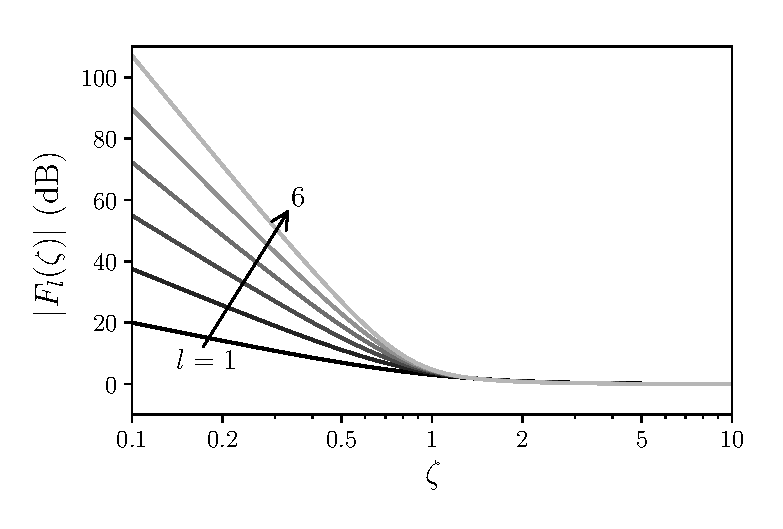
\includegraphics[width = 0.6\textwidth]{02_acoustical_theory/figures/nearfield_amplification.eps}
  \caption[Magnitudes of the family of functions given in \eqnref{eq:02_Acoustical_Theory:Fl_zeta}.]{
  Magnitudes of the family of functions given in \eqnref{eq:02_Acoustical_Theory:Fl_zeta} for increasing values of $l$ from $l = 1$ (black curve) to $6$ (lightest gray).
  If the nondimensional wavenumber $k s_0 / l$ is substituted for $\zeta$, then these curves illustrate the near-field amplification introduced when encoding a point-source into ambisonics (see \eqnref{eq:02_Acoustical_Theory:Nearfield_Amplification} and cf.~\citet[Fig.~4]{Daniel2003b}).}
  \label{fig:02_Acoustical_Theory:Nearfield_Amplification}
\end{figure}

If we let $\zeta = k s_0 / l$, we can relate this function to the distance-coding term of the point-source encoding filters (as given in \eqnref{eq:02_Acoustical_Theory:PointSource_An}) by
\begin{equation}\label{eq:02_Acoustical_Theory:Nearfield_Amplification}
\left| s_0 \frac{A_n (k)}{Y_n (\hat{s}_0)} \right| = \left| k s_0 h_l (k s_0) \right| = \left| F_l \left( \frac{k s_0}{l} \right) \right|,
\end{equation}
where $|\cdot|$ denotes the absolute value (or modulus or magnitude) of the argument.
From this relationship, we see that increasing (or decreasing) the source distance $s_0$ has two effects on the resulting ambisonics signals:
\begin{enumerate}
\item the overall amplitude of each ambisonics signal decreases (increases), and
\item the frequency below which the amplification occurs decreases (increases).
\end{enumerate}
In particular, the ambisonics signals are amplified at frequencies below $k = l / s_0$ (cf.~\citep[section 2.1]{Daniel2003b}).

To prevent excessive low-frequency amplification from this effect, we define for all ambisonics orders $l \in [1, L_\textrm{in}]$, an order-dependent, zero-phase high-pass Butterworth filter, the frequency response of which is given by
\begin{equation}\label{eq:02_Acoustical_Theory:NearField_HPF}
H_l(f) = 1 - \frac{1}{\sqrt{1 + \left( \frac{f}{f_l} \right)^l}},
\end{equation}
where $f_l$ is the corner frequency of the $l^\textrm{th}$ filter,
which, unless stated otherwise, we choose to be $f_l = (200 \times l)$~Hz.

As shown above, the frequency at which the near-field amplification occurs increases as the distance between the source and microphone decreases.
However, the compensation filters given in~\eqnref{eq:02_Acoustical_Theory:NearField_HPF} are independent of source position, which will lead to excessive low-frequency amplification (due to insufficient compensation) at small source distances and excessive low-frequency attenuation at large source distances.
The plots in \figref{fig:02_Acoustical_Theory:Nearfield_Compensation} illustrate this effect for $s_0 = 0.05, 1$~m.
This approach, while inexact, is representative of practical reality since, in general, the source position(s) may be unknown.
Indeed, the Eigenmike by mh acoustics uses distance-independent compensation filters \citep[section 4.3]{EigenUnitsManual2018}.
(In the experimental validation presented in \chapref{chap:10_Experimental_Validation}, we use distance-independent compensation filters to match those of the Eigenmike.)

\begin{figure}[t]
    \centering
    \begin{subfigure}[b]{0.49\textwidth}
        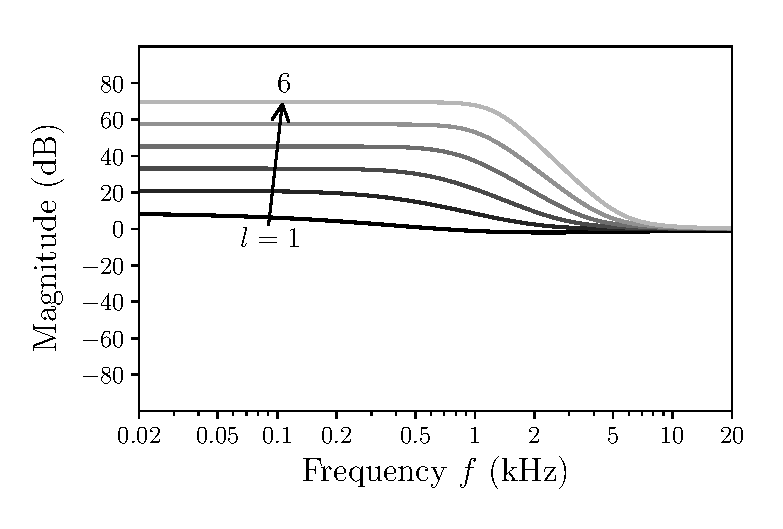
\includegraphics[width=\textwidth]{02_acoustical_theory/figures/nearfield_compensation_5cm.eps}
        \caption{$s_0 = 0.05$~m}
    \end{subfigure}
    \hfill
    \begin{subfigure}[b]{0.49\textwidth}
        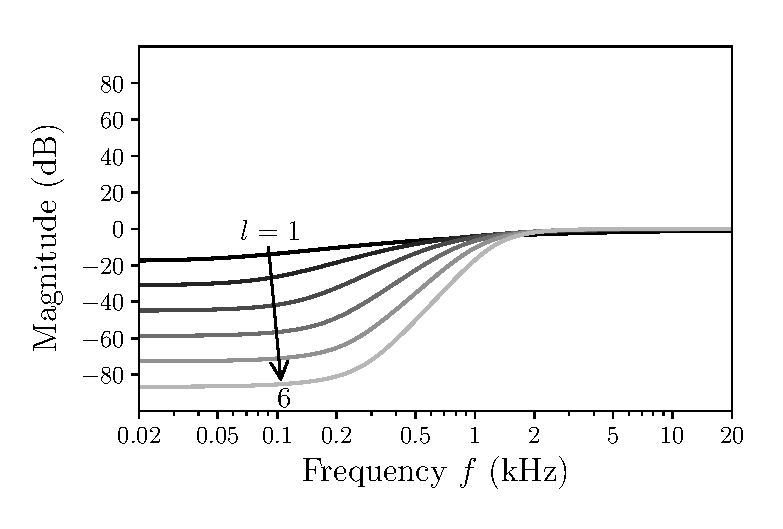
\includegraphics[width=\textwidth]{02_acoustical_theory/figures/nearfield_compensation_100cm.eps}
        \caption{$s_0 = 1$~m}
    \end{subfigure}
\caption[Residual near-field amplification after compensation.]{
Residual near-field amplification for two different source distances after compensation with the Butterworth high-pass filter (see \eqnref{eq:02_Acoustical_Theory:NearField_HPF}).
The magnitude spectra have been multiplied by $s_0$ in order to remove the vertical offset caused by the overall distance attenuation.}
\label{fig:02_Acoustical_Theory:Nearfield_Compensation}
\end{figure} %%NOTE%% vertical axis label is too complicated: |A H| s or something

\section{Plane-wave decomposition}\label{sec:02_Acoustical_Theory:Plane-Wave_Expansion}
Given spherical Fourier-Bessel expansion coefficients, $A_n$, the so-called \textit{signature function}, $\mu$, in the direction $\hat{v}_q$ is given by~\citep[section~2.3.3]{GumerovDuraiswami2005}
\begin{equation}\label{eq:02_Acoustical_Theory:A2mu}
\mu(k,\hat{v}_q) = \sum_{n=0}^{N-1} A_n(k) \frac{Y_n(\hat{v}_q)}{\left\|Y_n\right\|^2}.
\end{equation}
This computation of the signature function is often referred to as \textit{modal beamforming},%
\footnote{This is as opposed to \textit{delay-and-sum beamforming}, in which the appropriately-delayed signals from each individual microphone capsule in an array are summed to isolate the signals from a desired incident direction (which will be added in-phase) while cancelling signals arriving from other directions.}
as the process amounts to an isolation of the sound coming from the direction $\hat{v}_q$ (the so-called ``look direction'') via a linear combination of the different spherical ``modes'' of the sound field (cf.~\citet{HahnSpors2015b,Spors2012}).

The signature function represents the coefficients of a plane-wave decomposition of the sound field, such that the potential field can be approximately reconstructed using a finite number of plane-waves.%
\footnote{Alternatively, the signature function can be computed using a pseudoinverse of a matrix of spherical harmonics, as described in \eqnref{eq:02_Acoustical_Theory:A2mu_Pinv}.}
Assuming that the spherical Fourier-Bessel expansion was taken about the origin, this reconstructed potential field is given by
\begin{equation}\label{eq:02_Acoustical_Theory:PW_Quadrature_Rendered_Field}
\psi(k,\vec{r}) \approx \sum_{q=1}^Q w_q \mu(k,\hat{v}_q) e^{-i k \hat{v}_q \cdot \vec{r}},
\end{equation}
where $Q$ is the number of plane-wave terms, $\hat{v}_q$ is the source direction of the $q^\text{th}$ term, and $w_q$ is its quadrature weight, which is dependent on the chosen grid of directions.
By convention, we assume $\sum_{q=1}^Q w_q \approx 4 \pi$, and typically require that $w_q \neq 0,~\forall q \in [1, Q]$.

The signature function can be converted back into ambisonics signals, given by
\begin{equation}\label{eq:02_Acoustical_Theory:mu2A_Quadrature}
A_n(k) = \sum_{q=1}^{Q} w_q \mu(k,\hat{v}_q) Y_{n}(\hat{v}_q),
\end{equation}
where we have essentially encoded the sum of $Q$ plane-wave signals via \eqnref{eq:02_Acoustical_Theory:PlaneSource_An}.

\section{Ambisonics translation coefficients}\label{sec:02_Acoustical_Theory:Ambisonics_Translation}
Let $R_n(k, \vec{r})$ denote the spherical Fourier-Bessel basis functions defined in \secref{sec:02_Acoustical_Theory:Helmholtz_Equation} (see \eqnref{eq:02_Acoustical_Theory:Infinite_Order_Expansion}) and given by
\begin{equation}\label{eq:02_Acoustical_Theory:Basis_Functions}
R_n(k, \vec{r}) = 4\pi (-i)^l j_l(kr) \frac{Y_n(\hat{r})}{\|Y_n\|^2}.
\end{equation}
It can be shown that these basis functions can be translated along the vector $\vec{r}_0$ by \citep[Eq.~(3.2.1)]{GumerovDuraiswami2005}
\begin{equation}\label{eq:02_Acoustical_Theory:Translated_Basis_Functions}
R_n(k, \vec{r} + \vec{r}_0) = \sum_{n' = 0}^\infty T_{n,n'}(k,\vec{r}_0) R_{n'}(k, \vec{r}),
\end{equation}
where $T_{n,n'}$ are the so-called \textit{translation coefficients}.
Integral forms of these translation coefficients as well as fast recurrence relations for computing them are given by \citet[section~3.2]{GumerovDuraiswami2005} and \citet[chapter 3]{Zotter2009PhD}.
Additionally, a distilled algorithm for computing these coefficients is given by \citet{TylkaChoueiri2019a}, which is reproduced in \apxref{chap:A1_Navigation_Filters} of the present thesis.

Now let us consider two sets of spherical Fourier-Bessel expansion coefficients for the same sound field: $B_n$, which describe the sound field for an expansion about the origin, and $A_{n'}$, which do the same for an expansion about $\vec{r}_0$.
By \eqnref{eq:02_Acoustical_Theory:Infinite_Order_Expansion}, the acoustic potential field is given by
\begin{equation}
\psi(k,\vec{r} + \vec{r}_0) = \sum_{n' = 0}^\infty A_{n'}(k) R_{n'}(k, \vec{r}) = \sum_{n = 0}^\infty B_n(k) R_n(k, \vec{r} + \vec{r}_0).
\end{equation}
Substituting \eqnref{eq:02_Acoustical_Theory:Translated_Basis_Functions} into the above equation yields
\begin{equation}
\sum_{n' = 0}^\infty A_{n'}(k) R_{n'}(k, \vec{r}) = \sum_{n = 0}^\infty B_n(k) \left[ \sum_{n' = 0}^\infty T_{n,n'}(k,\vec{r}_0) R_{n'}(k, \vec{r}) \right].
\end{equation}
Rearranging and interchanging the order of the summations%
\footnote{Note that this is possible when the summations converge absolutely and uniformly \citep[section 3.1.1]{GumerovDuraiswami2005}, which is likely the case since the expression necessarily converges to a finite $\psi$ for real sound fields.
In any case, since in practice these summations will be truncated at a finite order, swapping the order becomes trivial.}
reveals
\begin{align}
\sum_{n' = 0}^\infty A_{n'}(k) R_{n'}(k, \vec{r}) &= \sum_{n' = 0}^\infty \left[ \sum_{n = 0}^\infty T_{n,n'}(k,\vec{r}_0) B_n(k) \right] R_{n'}(k, \vec{r}), \\
\implies A_{n'}(k) &= \sum_{n = 0}^\infty T_{n,n'}(k, \vec{r}_0) B_n(k).
\end{align}

In practice, we have only a truncated series expansion of the sound field, with measured coefficients $B_n$ up to order $L$, such that we compute
\begin{equation}\label{eq:02_Acoustical_Theory:Translated_Expansion_Coefficients}
A_{n'}(k) = \sum_{n = 0}^{N-1} T_{n,n'}(k, \vec{r}_0) B_n(k),
\end{equation}
where $N = (L + 1)^2$.
This translation process is illustrated in \figref{fig:03_Navigation_Techniques:Problem_Formulation} for an arbitrary original expansion center, $\vec{u}$.
Note that the translated expansion coefficients $A_{n'}$ can be computed to an arbitrary order $L'$, with $N' = (L' + 1)^2$ terms.

In matrix form, we can write \eqnref{eq:02_Acoustical_Theory:Translated_Expansion_Coefficients} as
\begin{equation}\label{eq:02_Acoustical_Theory:Translated_Expansion_Coefficients_Matrix}
\mathbf{a}(k) = \left( \mathbf{T}(k, \vec{r}_0) \right)^\text{T} \cdot \mathbf{b}(k),
\end{equation}
where $(\cdot)^\text{T}$ denotes the transpose of the argument and, omitting dependencies,
\begin{equation}\label{eq:02_Acoustical_Theory:Expansion_Coefficients_Vectors}
\mathbf{a} = 
    \left[ \begin{array}{c}
    A_0\\
    A_1\\
    \vdots\\
    A_{N'-1}
    \end{array} \right]
,\quad
\mathbf{b} = 
    \left[ \begin{array}{c}
    B_0\\
    B_1\\
    \vdots\\
    B_{N-1}
    \end{array} \right],
\end{equation}
and
\begin{equation}\label{eq:02_Acoustical_Theory:Translation_Matrix}
\mathbf{T}_{(N \times N')} = 
    \left[ \begin{array}{cccc}
    T_{0,0} & T_{0,1} & \cdots & T_{0,N'-1}\\
    T_{1,0} & T_{1,1} & \cdots & T_{1,N'-1}\\
    \vdots & \vdots & \ddots & \vdots\\
    T_{N-1,0} & T_{N-1,1} & \cdots & T_{N-1,N'-1}
    \end{array} \right].
\end{equation}
An algorithm to compute this matrix via recurrence relations is given in~\apxref{chap:A1_Navigation_Filters}.

\section{Rendering (decoding) ambisonics to binaural}\label{sec:02_Acoustical_Theory:Binaural_Rendering}
Generally, binaural decoding of ambisonics aims to generate the appropriate binaural signals for a listener at a point (with any orientation) in a recorded (or synthesized) sound field,
such that the resulting perception of the sound field is identical to that which would have occurred in the real sound field.
At the origin, this task may be accomplished by:
\begin{enumerate}
\item decoding the ambisonics signals to a fixed set of virtual loudspeakers and filtering each loudspeaker's signal by the appropriate HRTF \citep{McKeagMcGrath1996,Noisternig2003a},
\item transforming the ambisonics signals into a plane-wave expansion of the sound field and filtering each plane-wave term by the appropriate HRTF \citep{Duraiswami2005a,MenziesAlAkaidi2007b}, 
\item using a spherical-harmonic decomposition of the listener's HRTFs to filter each ambisonics signal directly \citep{RafaelyAvni2010,Bernschutz2014}, or
\item decomposing the (typically first-order only) ambisonics signals into directional (and diffuse) components using non-linear, parametric techniques (e.g., HARPEX, DirAC) and filtering each component by the appropriate HRTF \citep{Laitinen2008,BergeBarrett2010b}.
\end{enumerate}
In this section, we review the first three approaches listed above.
A corresponding MATLAB toolkit developed by the present author which implements these first three approaches is presented in \apxref{chap:A2_SABRE_Toolkit}.

\subsection{Virtual ambisonics}\label{sec:02_Acoustical_Theory:VA_Binaural}
Generally, the ambisonics decoding matrix, $\mathbf{D}$, which is typically time- and frequency-independent,%
\footnote{Although two- or multi-band decoders are commonly used, the decoder matrix for each sub-band is typically time-independent \citep{Heller2012}.}
determines the loudspeaker signals, $g_q$, given by
\begin{equation}\label{eq:02_Acoustical_Theory:Ambisonics_Decoding}
\mathbf{g}(t) = 
\begin{bmatrix}
g_{1}(t) \\ g_{2}(t) \\ \vdots \\ g_{Q}(t)
\end{bmatrix}
 = \mathbf{D} \cdot 
\begin{bmatrix}
a_{0}(t) \\ a_{1}(t) \\ \vdots \\ a_{N-1}(t)
\end{bmatrix}
 = \mathbf{D} \cdot \mathbf{a}(t),
\end{equation}
where $Q$ is the number of loudspeakers and $a_n$ is the $n^\text{th}$ ambisonics signal.
Methods of calculating the decoding matrix have been extensively researched and it is outside of the scope of this thesis to discuss them in detail.
Briefly, the decoding matrix attempts to use all available loudspeakers to create a perceptually-accurate reproduction the recorded sound field \citep{Heller2012}.

Following traditional ambisonic theory,
we consider the ambisonics signals produced at the center of the loudspeaker array
in response to the loudspeaker signals, given by
\begin{equation}
a_n(t) = \sum_{q=1}^{Q} Y_{n}(\hat{v}_q) g_q(t).
\end{equation}
(Note that this effectively treats the loudspeakers as plane-wave sources via \eqnref{eq:02_Acoustical_Theory:PlaneSource_An}.)
Equivalently, in matrix form, we have $\mathbf{a}(t) = \mathbf{Y} \cdot \mathbf{g}(t)$, where
\begin{equation}\label{eq:YMatrix}
\mathbf{Y} = 
\begin{bmatrix}
Y_{0}(\hat{v}_1) & Y_{0}(\hat{v}_2) & \cdots & Y_{0}(\hat{v}_Q) \\
Y_{1}(\hat{v}_1) & Y_{1}(\hat{v}_2) & \cdots & Y_{1}(\hat{v}_Q) \\
\vdots & \vdots & \ddots & \vdots \\
Y_{N-1}(\hat{v}_1) & Y_{N-1}(\hat{v}_2) & \cdots & Y_{N-1}(\hat{v}_Q)
\end{bmatrix}.
\end{equation}
From this formulation, we obtain the basic (pseudoinverse) decoder, given by \citep[Appendix~A.1]{Heller2008}
\begin{equation}\label{eq:02_Acoustical_Theory:PinvDecoder}
\mathbf{D} = \mathbf{Y}^{+},
\end{equation}
where $(\cdot)^{+}$ denotes pseudoinversion.
For a thorough review of ambisonic decoding theory and practice,
the reader is referred to the works of \citeauthor{Heller2008}~\citep{Heller2008,Heller2012}.

Assuming a free field and ideal loudspeakers that are equidistant from the listener,
the resulting binaural pressure signals are given by
\begin{equation}\label{eq:02_Acoustical_Theory:VA_Binaural}
p^{\text{L,R}}(t) = \left( \mathbf{h}^{\text{L,R}} \ast \mathbf{g} \right)(t)
 = \sum_{q=1}^Q \left( h_{q}^{\text{L,R}} \ast g_{q} \right) (t),
\end{equation}
where `$\ast$' denotes convolution (which, for matrices and vectors operates like matrix multiplication except each pair of elements is convolved rather than multiplied) and
\begin{equation}
\mathbf{h}^{\text{L,R}}(t) = 
\begin{bmatrix}
h_{1}^{\text{L,R}}(t) & h_{2}^{\text{L,R}}(t) & \cdots & h_{Q}^{\text{L,R}}(t)
\end{bmatrix}
\end{equation}
is a vector containing the head-related impulse responses (HRIRs) for a given listener
and for the directions of each loudspeaker.
The superscript ``$\text{L,R}$'' denotes the response at the left or right ear, respectively.
Combining \eqnreftwo{eq:02_Acoustical_Theory:Ambisonics_Decoding}{eq:02_Acoustical_Theory:VA_Binaural},
we obtain a simple matrix expression for rendering ambisonics to binaural, given by
\begin{equation}\label{eq:02_Acoustical_Theory:VA_Binaural_Matrix}
p^{\text{L,R}}(t) = \left( \mathbf{h}^{\text{L,R}} \ast \left( \mathbf{D} \cdot \mathbf{a} \right) \right)(t).
\end{equation}

\subsection{Plane-wave rendering}\label{sec:02_Acoustical_Theory:PW_Quadrature_Binaural}
For this rendering approach, we first compute the signature function, $\mu$, of the sound field,
as given by \eqnref{eq:02_Acoustical_Theory:A2mu}.
Equivalently, written as a matrix equation, we have
\begin{equation}\label{eq:02_Acoustical_Theory:A2mu_Matrix}
\mathbf{m}(t) = 
\begin{bmatrix}
\mu(t,\hat{v}_1) \\ \mu(t,\hat{v}_2) \\ \vdots \\ \mu(t,\hat{v}_Q)
\end{bmatrix} 
= \mathbf{Y}^{\textrm{T}} \cdot \mathbf{F}^{-1} \cdot \mathbf{a}(t),
\end{equation}
where $Q$ is now the number of plane-wave terms and $\mathbf{F}$ is a diagonal matrix given by
\begin{equation}
\mathbf{F} = \text{diag} \left\{ \begin{bmatrix} \left\|Y_0\right\|^{2} & \left\|Y_1\right\|^{2} & \cdots & \left\|Y_{N-1}\right\|^{2} \end{bmatrix} \right\}.
\end{equation}

Given the signature function, the binaural pressure signals can be approximately reconstructed using a finite number of plane-waves, given by \citep{Duraiswami2005a}
\begin{equation}\label{eq:02_Acoustical_Theory:PW_Quadrature_Binaural}
p^{\text{L,R}}(t) \approx \sum_{q=1}^Q \left( h_{q}^{\text{L,R}} \ast \left(w_q \mu(\hat{v}_q) \right) \right) (t)
 = \left(\mathbf{h}^{\text{L,R}} \ast \left( \mathbf{W} \cdot \mathbf{m} \right) \right)(t),
\end{equation}
where $w_q$ is the quadrature weight of the $q^\textrm{th}$ plane-wave term and we have let
\begin{equation}\label{eq:02_Acoustical_Theory:PW_Quadrature_Weights}
\mathbf{W} = \text{diag} \left\{ \begin{bmatrix} w_1 & w_2 & \cdots & w_Q \end{bmatrix} \right\}.
\end{equation}
Combining \eqnreftwo{eq:02_Acoustical_Theory:A2mu_Matrix}{eq:02_Acoustical_Theory:PW_Quadrature_Binaural}, we obtain
\begin{equation}\label{eq:02_Acoustical_Theory:PW_Quadrature_Binaural_Matrix}
p^{\text{L,R}}(t) = \left( \mathbf{h}^{\text{L,R}} \ast \left( \mathbf{W} \cdot \mathbf{Y}^{\textrm{T}} \cdot \mathbf{F}^{-1} \cdot \mathbf{a} \right) \right) (t).
\end{equation}

It is worth noting that, instead of using \eqnref{eq:02_Acoustical_Theory:A2mu_Matrix}, we can compute $\mu$ following the pseudoinverse approach of \eqnref{eq:02_Acoustical_Theory:PinvDecoder}, such that
\begin{equation}\label{eq:02_Acoustical_Theory:A2mu_Pinv}
\mathbf{m}(t) = \mathbf{W}^{-1} \cdot \mathbf{Y}^{+} \cdot \mathbf{a}(t).
\end{equation}
Combining \eqnreftwo{eq:02_Acoustical_Theory:PW_Quadrature_Binaural}{eq:02_Acoustical_Theory:A2mu_Pinv}, we obtain
\begin{equation}\label{eq:02_Acoustical_Theory:PW_Pinv_Binaural_Matrix}
p^{\text{L,R}}(t) = \left( \mathbf{h}^{\text{L,R}} \ast \left( \mathbf{Y}^{+} \cdot \mathbf{a} \right) \right) (t).
\end{equation}
However, this results in identical binaural signals (assuming the same grid of $Q$ directions) between \eqnreftwo{eq:02_Acoustical_Theory:VA_Binaural_Matrix}{eq:02_Acoustical_Theory:PW_Pinv_Binaural_Matrix}, since we have effectively set $w_q \mu(t,\hat{v}_q) = g_q(t)$.

\subsection{Spherical-harmonic HRTFs}\label{sec:02_Acoustical_Theory:SH_Binaural}
A more computationally efficient approach to rendering ambisonics to binaural is to filter each ambisonics signal by the corresponding term in a spherical-harmonic decomposition of an HRTF.
The spherical-harmonic HRTFs can be computed via pseudoinverse, as given by \citet[section IV]{RafaelyAvni2010}, such that
\begin{equation}\label{eq:02_Acoustical_Theory:SH_HRTFs}
\mathbf{\tilde{h}}^{\text{L,R}}(t) = 
\begin{bmatrix}
\tilde{h}_{0}^{\text{L,R}}(t) & \tilde{h}_{1}^{\text{L,R}}(t) & \cdots & \tilde{h}_{N-1}^{\text{L,R}}(t)
\end{bmatrix}
 = \mathbf{h}^{\text{L,R}}(t) \cdot \mathbf{Y}^{+}.
\end{equation}
The resulting binaural pressure signals are then given by
\begin{equation}\label{eq:02_Acoustical_Theory:SH_Binaural}
p^{\text{L,R}}(t) \approx \sum_{n=0}^{N-1} \left( \tilde{h}_n^{\text{L,R}} \ast a_n \right) (t)
 = \left( \mathbf{\tilde{h}}^{\text{L,R}} \ast \mathbf{a} \right) (t).
\end{equation}
Combining~\eqnreftwo{eq:02_Acoustical_Theory:SH_HRTFs}{eq:02_Acoustical_Theory:SH_Binaural}, we obtain
\begin{equation}\label{eq:02_Acoustical_Theory:SH_Binaural_Matrix}
p^{\text{L,R}}(t) = \left( \left( \mathbf{h}^{\text{L,R}} \cdot \mathbf{Y}^{+} \right) \ast \mathbf{a} \right) (t),
\end{equation}
which is identical (again, assuming the same grid of $Q$ directions) to both \eqnreftwo{eq:02_Acoustical_Theory:VA_Binaural_Matrix}{eq:02_Acoustical_Theory:PW_Pinv_Binaural_Matrix}.
%%%% NAVIGATIONAL TECHNIQUES %%%%
\chapter{Review of existing navigational methods}\label{chap:03_Navigation_Techniques}
As mentioned in \secref{sec:01_Introduction:Background}, the goal of virtual navigation is to reconstruct, at a specified position (e.g., the location of a listener), a sound field that has been measured from one or more known locations (e.g., the locations of ambisonics microphones).
In this section, we review existing methods for such virtual navigation of ambisonics-encoded sound fields.
The methods reviewed here are listed in \tabref{tab:01_Introduction:Methods} (although not all those methods listed in the table are reviewed here).
We first present a general mathematical formulation of the navigation problem in \secref{sec:03_Navigation_Techniques:Problem_Formulation} in order to establish a consistent framework and nomenclature for describing the methods.
We then describe several existing navigational methods: in \secref{sec:03_Navigation_Techniques:Extrapolation_Methods}, we present three linear extrapolation-based navigational methods and, in \secref{sec:03_Navigation_Techniques:Interpolation_Methods}, we present three (two linear and one parametric) interpolation-based navigational methods.
The performance of several of these methods will be characterized in \chaprefthru{chap:07_Characterization_Extrapolation}{chap:09_Thiergart_Comparison}.
%Several of these methods have also been implemented in a MATLAB toolkit, which is freely available online.\citefooturl{AmbiNavToolkitURL}

\section{Mathematical formulation}\label{sec:03_Navigation_Techniques:Problem_Formulation}
Generally, we seek the ambisonics signals, $a_n$, up to order $L_\text{out}$, that describe the sound field in the vicinity of the listener, located at $\vec{r}_0$.
Using \eqnref{eq:02_Acoustical_Theory:Finite_Order_Expansion}, this potential field is given by
\begin{equation}\label{eq:03_Navigation_Techniques:Output_Potential_Field}
\psi(k,\vec{r} + \vec{r}_0) = \sum_{n=0}^{N_\text{out} - 1} 4\pi (-i)^l A_n(k) j_l(kr) \frac{Y_n(\hat{r})}{\|Y_n\|^2} ,
\end{equation}
where $N_\text{out} = (L_\text{out} + 1)^2$ and $A_n = \mathcal{F} \left[ a_n \right]$.

We take as inputs to each navigational method a set of measured (or synthesized) ambisonics signals, $b_n$, up to order $L_\text{in}$, that describe the sound field in the vicinity of the microphone (either real or virtual), which is located at $\vec{u}$.
Again using \eqnref{eq:02_Acoustical_Theory:Finite_Order_Expansion}, this potential field is given by
\begin{equation}\label{eq:03_Navigation_Techniques:Input_Potential_Field}
\psi(k,\vec{r} + \vec{u}) = \sum_{n=0}^{N_\text{in} - 1} 4\pi (-i)^l B_n(k) j_l(kr) \frac{Y_n(\hat{r})}{\|Y_n\|^2} ,
\end{equation}
where $N_\text{in} = (L_\text{in} + 1)^2$ and $B_n = \mathcal{F} \left[ b_n \right]$.
Thus, estimation of $a_n$ from $b_n$ amounts to a translation from the position of the microphone, $\vec{u}$, along the vector $\vec{r}_0 - \vec{u}$, as illustrated in \figref{fig:03_Navigation_Techniques:Problem_Formulation}.

% Diagram of source/mic positions
\begin{figure}[t]
\centering
  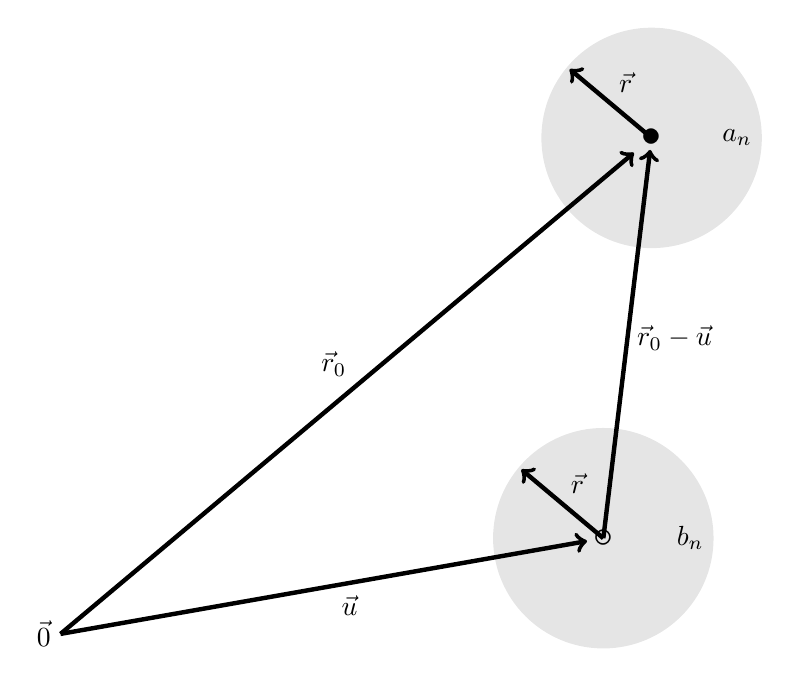
\begin{tikzpicture}[scale=5]
% Parameters
\def\lengthscale{1.4};
\def\radius{0.2*\lengthscale}
\def\arrowStart{0};
\def\arrowScale{0.97};

\pgfmathsetmacro\evalX{cos(140)*\radius}
\pgfmathsetmacro\evalY{sin(140)*\radius}

\pgfmathsetmacro\micX{cos(10)*\lengthscale}
\pgfmathsetmacro\micY{sin(10)*\lengthscale}

\pgfmathsetmacro\listenerX{cos(40)*1.4*\lengthscale}
\pgfmathsetmacro\listenerY{sin(40)*1.4*\lengthscale}

% Arrows
%\draw[ultra thick,->] ({\arrowStart*\evalX},{\arrowStart*\evalY}) -- (\arrowScale*\evalX,\arrowScale*\evalY);
%\node[above right] at (0.5*\evalX,0.5*\evalY){$\vec{r}$};
%\fill [color=black,opacity=0.1] (0,0) circle (\radius);

\draw[ultra thick,->] ({\arrowStart*\evalX+\micX},{\arrowStart*\evalY+\micY}) -- (\arrowScale*\evalX+\micX,\arrowScale*\evalY+\micY);
\node[above right] at (0.5*\evalX+\micX,0.5*\evalY+\micY){$\vec{r}$};
\fill [color=black,opacity=0.1] (\micX,\micY) circle (\radius);

\draw[ultra thick,->] ({\arrowStart*\evalX+\listenerX},{\arrowStart*\evalY+\listenerY}) -- (\arrowScale*\evalX+\listenerX,\arrowScale*\evalY+\listenerY);
\node[above right] at (0.5*\evalX+\listenerX,0.5*\evalY+\listenerY){$\vec{r}$};
\fill [color=black,opacity=0.1] (\listenerX,\listenerY) circle (\radius);

\draw[ultra thick,->] ({\arrowStart*\micX},{\arrowStart*\micY}) -- (\arrowScale*\micX,\arrowScale*\micY);
\node[below right] at (0.5*\micX,0.5*\micY){$\vec{u}$};

\draw[ultra thick,->] ({\arrowStart*\listenerX},{\arrowStart*\listenerY}) -- (\arrowScale*\listenerX,\arrowScale*\listenerY);
\node[above left] at (0.5*\listenerX,0.5*\listenerY){$\vec{r}_0$};

\draw[ultra thick,->] ({(\listenerX-\micX)*\arrowStart+\micX},{(\listenerY-\micY)*\arrowStart+\micY}) -- ({(\listenerX-\micX)*\arrowScale+\micX},{(\listenerY-\micY)*\arrowScale+\micY});
\node[right] at ({(\listenerX-\micX)*0.5+\micX},{(\listenerY-\micY)*0.5+\micY}){$\vec{r}_0 - \vec{u}$};

% Origin
\node[left] at (0,0){$\vec{0}$};

% Mic position
\node at (\micX,\micY){\Large $\circ$};
\node[left] at (\micX+\radius,\micY){$b_n$};

% Listener position
\node at (\listenerX,\listenerY){\Large $\bullet$};
\node[left] at (\listenerX+\radius,\listenerY){$a_n$};
\end{tikzpicture}
  \caption[Diagram of microphone and listener positions.]{
  Diagram of microphone and listener positions.
  The empty circle indicates the microphone position,
  the filled circle indicates the listener position, and
  the shaded disks indicate the regions of the sound field represented by the corresponding ambisonics expansions.}
  \label{fig:03_Navigation_Techniques:Problem_Formulation}
\end{figure}

In general, we will consider arrays of $P$ ambisonics microphones, where the $p^\text{th}$ microphone is located at $\vec{u}_p$ for $p \in [1,P]$.
For microphones of order $L_\text{in}$,\footnote{The order of the ambisonics microphone is generally determined by the number of capsules in the assembly.} each microphone captures $N_\text{in} = (L_\text{in} + 1)^2$ ambisonics signals, which we represent with a vector, $\mathbf{b}_p$.
(See \chapref{chap:02_Acoustical_Theory} for a review of ambisonics conventions and theory.)
%In general, ambisonics navigation techniques aim to approximate, up to order $L_\text{out}$ and with $N_\text{out} = (L_\text{out} + 1)^2$ terms, the exact ambisonics signals, $\mathbf{a}$, of the sound field at a listening position $\vec{r}_0$.
In the case of extrapolation methods, for which $P = 1$, we omit the subscripts for $\vec{u}_1$ and $\mathbf{b}_1$ (and instead simply use $\vec{u}$ and $\mathbf{b}$, respectively).

% include operator notation, tikz block diagram

\section{Extrapolation methods}\label{sec:03_Navigation_Techniques:Extrapolation_Methods}
In this section, we review three linear extrapolation-based navigational methods:
\begin{enumerate}
\item virtual ambisonics \citep[section 3.1]{TylkaChoueiri2015},
\item plane-wave translation \citep{SchultzSpors2013}, and
\item ambisonics translation \citep{GumerovDuraiswami2005,MenziesAlAkaidi2007a,Zotter2009PhD}.
\end{enumerate}

%% VIRTUAL AMBISONICS %%
\subsection{Virtual ambisonics}\label{sec:03_Navigation_Techniques:VA_Technique}
The first navigational method we consider involves simulating ambisonics playback over a virtual array of loudspeakers (hereafter called ``virtual ambisonics'').
In this case, virtual navigation requires only that each loudspeaker signal be appropriately attenuated and delayed based on the distance of the listener to that loudspeaker.
The process of decoding ambisonics signals of order $L_\text{in}$ to $Q$ loudspeakers is reviewed in \secref{sec:02_Acoustical_Theory:VA_Binaural}, which converts the $N_\text{in}$ recorded ambisonics signals, $b_n$, into a set of loudspeaker signals, $g_q$.

Here we model the virtual loudspeakers as point-sources,\footnote{Note that we could have instead modeled the loudspeakers as plane-wave sources, infinitely far away from the listener. However, we chose to use finite-distance virtual loudspeakers so that this technique will differ more significantly from the plane-wave expansion technique described in \secref{sec:03_Navigation_Techniques:PW_Technique}.} where the $q^\text{th}$ loudspeaker is placed at $\vec{v}_q$ and is driven with a (Fourier-transformed) signal $G_q = \mathcal{F} \left[ g_q \right]$.
%Each loudspeaker then produces a potential field given by
%\begin{equation}\label{eq:03_Navigation_Techniques:Point_Source}
%\psi_q(k,\vec{r}) = \frac{e^{i k \left\| \vec{r} - \vec{v}_q \right\|}}{\left\| \vec{r} - \vec{v}_q \right\|} G_q(k),
%\end{equation}
%where we have used \eqnref{eq:02_Acoustical_Theory:PointSource}.
%The total potential field produced by virtual ambisonics playback is then given by
%\begin{equation}\label{eq:03_Navigation_Techniques:VA_Rendered_Field}
%\psi(k,\vec{r}) = \sum_{q = 1}^Q \frac{e^{i k \left\| \vec{r} - \vec{v}_q \right\|}}{\left\| \vec{r} - \vec{v}_q \right\|} G_q(k).
%\end{equation}
These signals are then re-encoded into ambisonics up to an arbitrary order, $L_\text{out}$, at the position of the listener, $\vec{r}_0$, via \eqnref{eq:02_Acoustical_Theory:PointSource_An}, such that
\begin{equation}\label{eq:03_Navigation_Techniques:VA_Output}
A_n(k) = \sum_{q = 1}^Q i^{l+1} k h_l(k \left\| \vec{v}_q - \vec{r}_0 \right\|) Y_n \left( \frac{\vec{v}_q - \vec{r}_0}{\left\| \vec{v}_q - \vec{r}_0 \right\|} \right) G_q(k).
\end{equation}

Note that, for binaural playback, we can skip the step of re-encoding to ambisonics and instead simply filter the point-source signals (appropriately attenuated and delayed based on distance to the listener) by the corresponding HRTFs of the listener.
However, for mathematical consistency when comparing different navigational methods, we choose an ambisonics output.

%To binaurally render the sound field described by~\eqnref{eq:03_Navigation_Techniques:VA_Rendered_Field} for a listener at position $\vec{r}_0$, the left and right binaural potentials (indicated by the superscripts ``$\text{L}$'' and ``$\text{R}$,'' respectively) are computed by
%\begin{equation}\label{eq:VA_Binaural}
%\psi_\text{VA}^\text{L,R}(k,\vec{r}_0) = \sum_{q=1}^{Q} \frac{e^{i k \left\| \vec{v}_q - \vec{r}_0 \right\|}}{\left\| \vec{v}_q - \vec{r}_0 \right\|} G_q(k) \cdot H^\text{L,R} \left( k, \frac{\vec{v}_q - \vec{r}_0}{\left\| \vec{v}_q - \vec{r}_0 \right\|} \right),
%\end{equation}
%where $H^\text{L,R}(k,\hat{v})$ is the far-field HRTF for a source in the direction $\hat{v}$.

%% PLANE-WAVE TRANSLATION %%
\subsection{Plane-wave translation}\label{sec:03_Navigation_Techniques:PW_Technique}
The second navigational method we consider uses a plane-wave decomposition of the finite-order potential field.
This technique was developed by \citet{SchultzSpors2013}, who showed that translation can be achieved by applying a frequency-domain phase-factor (or group delay in the time domain) to each plane-wave term, based on the direction of travel of the listener relative to the propagation direction of each plane-wave.

Beginning with \eqnref{eq:02_Acoustical_Theory:PW_Quadrature_Rendered_Field}, we see that, for each term in this summation, the potential field at $\vec{r} + \vec{r}_0$ differs only by a phase-factor: $e^{-i k \hat{v}_q \cdot \vec{r}_0}$.
We combine this factor into the signature function to define the \textit{translated signature function}, $\mu'$, given by \citep{MenziesAlAkaidi2007b}
\begin{equation}\label{eq:03_Navigation_Techniques:PW_Translation}
\mu'(k,\hat{v}_q;\vec{r}_0) = \mu(k,\hat{v}_q) e^{-i k \hat{v}_q \cdot \vec{r}_0},
\end{equation}
where the dot product in the exponential indicates that the $q^\text{th}$ plane-wave term undergoes a time delay proportional to the distance traveled parallel to the propagation direction, $-\hat{v}_q$, of that term.
Effectively, this operation translates the expansion center from the origin to $\vec{r}_0$.

Given a set of measured ambisonics signals, $\mathbf{b}$, up to order $L_\text{in}$, we can substitute $B_n$ for $A_n$ in \eqnref{eq:02_Acoustical_Theory:A2mu} to compute the measured signature function, $\mu$.
Then, using \eqnref{eq:03_Navigation_Techniques:PW_Translation},
we compute the translated signature function, $\mu'(k,\hat{v}_q;\vec{r}_0 - \vec{u})$,
where $\vec{u}$ is the position of the ambisonics microphone and $\vec{r}_0$ is the position of the listener.
By substituting $\mu'$ for $\mu$ in~\eqnref{eq:02_Acoustical_Theory:mu2A_Quadrature}, we then convert this translated signature function back into ambisonics signals, up to an arbitrary order, $L_\text{out}$, yielding ambisonics signals for the listener, $\mathbf{a}$.

Note that, as with the virtual ambisonics method, one could render the translated plane-wave terms directly to binaural by filtering each signal by the appropriate HRTF.
Here, however, we choose to generate an ambisonics output for mathematical consistency across different navigational methods.

%% AMBISONICS TRANSLATION %%
\subsection{Ambisonics translation}\label{sec:03_Navigation_Techniques:SR_Technique}
The third navigational method we consider was first described by \citet{MenziesAlAkaidi2007a}, and entails computing a new set of ambisonics signals by re-expanding the sound field about a translated expansion center using frequency-domain translation coefficients.

Following the theory described in \secref{sec:02_Acoustical_Theory:Ambisonics_Translation}, the ambisonics signals for the listener, $\mathbf{a}(k)$, are given by
\begin{equation}\label{eq:03_Navigation_Techniques:Forward_Ambisonics_Translation}
\mathbf{a}(k) = \left( \mathbf{T}(k, \vec{r}_0 - \vec{u}) \right)^\text{T} \cdot \mathbf{b}(k),
\end{equation}
where again $\vec{u}$ is the position of the ambisonics microphone (i.e., the expansion center for $\mathbf{b}$) and $\vec{r}_0$ is the position of the listener (cf.~\eqnref{eq:02_Acoustical_Theory:Translated_Expansion_Coefficients_Matrix}).
Recall that the translated expansion coefficients $A_n$ can be computed to an arbitrary order $L_\text{out}$.

The potential field at $\vec{r} + \vec{r}_0$ obtained through translation along $\vec{r}_0 - \vec{u}$ is then given by \eqnref{eq:03_Navigation_Techniques:Output_Potential_Field}.
It is important to note that the re-expanded field is still limited in accuracy and region of validity by the original expansion.
In other words, with increasing $L_\text{out}$, the re-expanded field approaches the original \textit{order-limited} field, not the incident field.

According to the inequality given in \eqnref{eq:01_Introduction:kr_Inequality}, the accuracy of the translated ambisonics signals will degrade with increasing frequency and distance away from the microphone.
To explore this behavior in the frequency domain, we compute the frequency response induced by translation away from the microphone and plot, in \figref{fig:03_Navigation_Techniques:SRE_RollOff}, the magnitude responses corresponding to various translation distances and input orders.%
\footnote{Simulations of this type are described in more detail in \chapref{chap:06_Simulation_Framework}.
Briefly, in this case, the sound field consists of a single point-source placed at $\vec{s}_0 = (2.5, 0, 0)$~m, a microphone of order $L_\text{in} \in [1,5]$ placed at $\vec{u} = (0.25, 0, 0)$~m, and a variable listener position of $\vec{r}_0 = (x_0, 0, 0)$ with $x_0 \in [0, 0.25]$~m.
A diagram of this geometry is shown in \figref{fig:06_Simulation_Framework:Point_Geometry}.
The microphone signals are given by \eqnref{eq:02_Acoustical_Theory:PointSource_An} and we have omitted the near-field compensation high-pass filter defined in \eqnref{eq:02_Acoustical_Theory:NearField_HPF}.
The effective frequency response induced by translating from $\vec{u}$ to $\vec{r}_0$ via \eqnref{eq:03_Navigation_Techniques:Forward_Ambisonics_Translation} is then given by the ratio of the translated zeroth-order ambisonics signal, $A_0(k)$, to the zeroth-order reference ambisonics signal, $B_0(k)$, that would have been measured at $\vec{r}_0$.}
From these plots, we see that translation effectively acts as a low-pass filter, the corner frequency of which approximately corresponds to $k \propto L_\text{in} / \| \vec{r}_0 - \vec{u} \|$.
(Although not shown here, it can be verified that this behavior also holds across all source and listener positions.
See, for example, \figref{fig:07_Characterization_Extrapolation:Azimuth_Dependence:SRE}, which shows this behavior over multiple source azimuths.)

\begin{figure}[t]
  \centering
  \begin{subfigure}[b]{0.49\textwidth}
    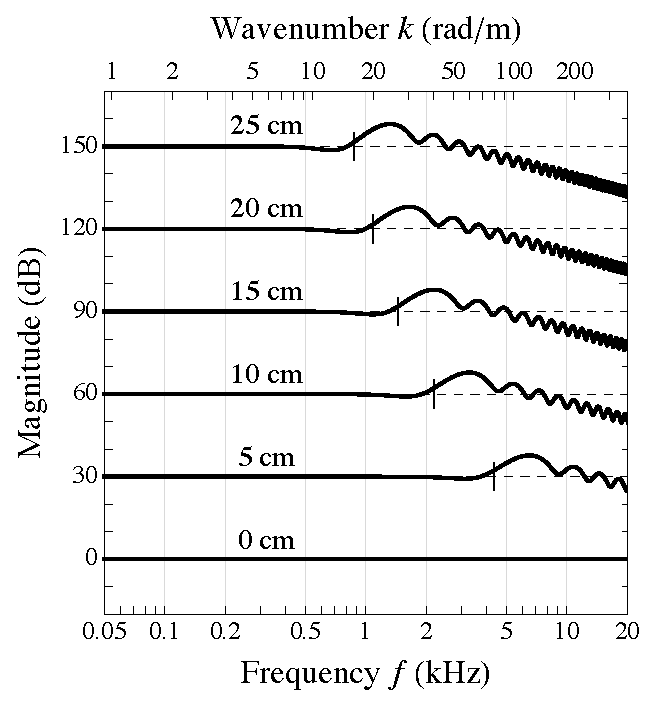
\includegraphics[width=\textwidth]{03_navigational_techniques/figures/freqResp_listenerPos_sre.eps}
    \caption{Varying $\| \vec{r}_0 - \vec{u} \|$; fixed $L_\text{in} = 4$}
    \label{fig:03_Navigation_Techniques:SRE_RollOff:ListenerPos}
  \end{subfigure}
  \hfill
  \begin{subfigure}[b]{0.49\textwidth}
    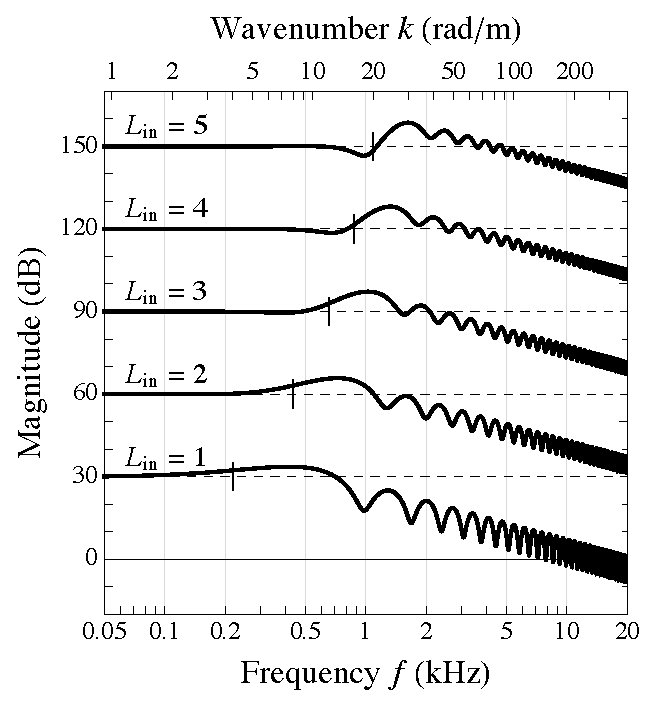
\includegraphics[width=\textwidth]{03_navigational_techniques/figures/freqResp_inputOrders_sre.eps}
    \caption{Varying $L_\text{in}$; fixed $\| \vec{r}_0 - \vec{u} \| = 0.25$~m}
    \label{fig:03_Navigation_Techniques:SRE_RollOff:InputOrders}
  \end{subfigure}
  \caption[Magnitude responses caused by the ambisonics translation method.]{
  Magnitude responses caused by the ambisonics translation method for various translation distances (left panel) and input orders (right).
  The bottom axes show frequency in kHz while the top axes show the angular wavenumber $k$.
  The short vertical lines indicate the nondimensional frequency $k \| \vec{r}_0 - \vec{u} \| = L_\text{in}$.
  For legibility, each frequency response is offset by $30$~dB.}
  \label{fig:03_Navigation_Techniques:SRE_RollOff}
\end{figure} %%NOTE%% vertical axis label is too complicated: |A0 / B0ref| or something

To better show the similarities across these different parameters, we plot, in \figref{fig:03_Navigation_Techniques:Nondim_SRE_RollOff}, the same magnitude responses as in \figref{fig:03_Navigation_Techniques:SRE_RollOff}, but now against a normalized wavenumber, $k \| \vec{r}_0 - \vec{u} \| / L_\text{in}$.
As expected, the corner of each effective low-pass filter is located at $k \| \vec{r}_0 - \vec{u} \| / L_\text{in} \approx 1$.
From these plots, we clearly see that the basic shape of the magnitude response is virtually identical across different translation distances (see \figref{fig:03_Navigation_Techniques:Nondim_SRE_RollOff:ListenerPos}), whereas varying the input order yields noticeable differences (\figref{fig:03_Navigation_Techniques:Nondim_SRE_RollOff:InputOrders}).
In particular, increasing the input order decreases the amplitude of, and spacing between, the ``ripples'' that modulate the overall low-pass behavior above the corner.

\begin{figure}[t]
  \centering
  \begin{subfigure}[b]{0.49\textwidth}
    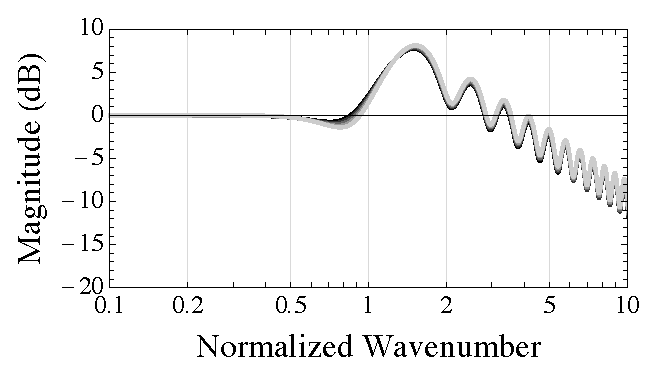
\includegraphics[width=\textwidth]{03_navigational_techniques/figures/nondimFreqResp_listenerPos_sre.eps}
    \caption{Varying $\| \vec{r}_0 - \vec{u} \|$; fixed $L_\text{in} = 4$}
    \label{fig:03_Navigation_Techniques:Nondim_SRE_RollOff:ListenerPos}
  \end{subfigure}
  \hfill
  \begin{subfigure}[b]{0.49\textwidth}
    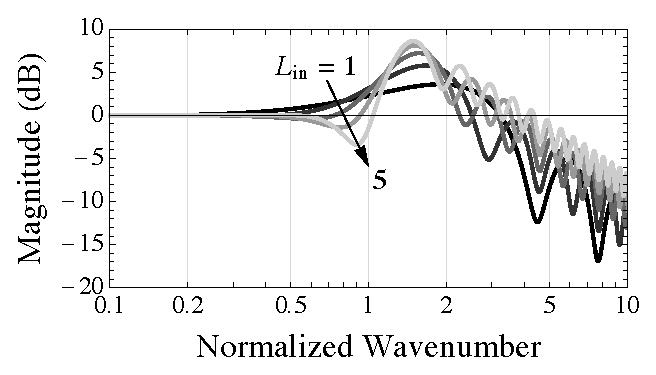
\includegraphics[width=\textwidth]{03_navigational_techniques/figures/nondimFreqResp_inputOrders_sre.eps}
    \caption{Varying $L_\text{in}$; fixed $\| \vec{r}_0 - \vec{u} \| = 0.25$~m}
    \label{fig:03_Navigation_Techniques:Nondim_SRE_RollOff:InputOrders}
  \end{subfigure}
  \caption[Magnitude responses caused by the ambisonics translation method.]{
  Magnitude responses caused by the ambisonics translation method for various translation distances (left panel) and input orders (right), where the lighter gray curves correspond to increasing translation distance or input order, respectively.
  The horizontal axes show the nondimensional wavenumber $k \| \vec{r}_0 - \vec{u} \| / L_\text{in}$.}
  \label{fig:03_Navigation_Techniques:Nondim_SRE_RollOff}
\end{figure}

It is worth noting that translation may also be carried out through the \textit{inverse} (or pseudoinverse if $L_\text{in} \neq L_\text{out}$) operation, such that
\begin{equation}\label{eq:03_Navigation_Techniques:Inverse_Ambisonics_Translation}
\mathbf{a}(k) = \left(\left( \mathbf{T}(k, \vec{u} - \vec{r}_0) \right)^\text{T} \right)^{-1} \cdot \mathbf{b}(k).
\end{equation}
However, as shown in \figref{fig:03_Navigation_Techniques:SRE_RollOff}, the forward translation operation given by~\eqnref{eq:03_Navigation_Techniques:Forward_Ambisonics_Translation} leads to an attenuation (i.e., a ``roll-off'') of high frequencies.
Consequently, the inverse operation will yield excessive high-frequency amplification, unless steps (such as regularization) are taken to mitigate such excessive gains.

In \secref{sec:03_Navigation_Techniques:Pinv_Technique}, a regularized least-squares approach is implemented in an interpolation method that uses multiple ambisonics microphones to estimate the ambisonics signals at the position of the listener.
Consequently, the inverse approach to extrapolation defined in \eqnref{eq:03_Navigation_Techniques:Inverse_Ambisonics_Translation} can be considered a special case of that interpolation method, in which we have only a single array (i.e., $P = 1$) and no regularization is used.

%%%% INTERPOLATION METHODS %%%%
\section{Interpolation methods}\label{sec:03_Navigation_Techniques:Interpolation_Methods}
In this section, we review three interpolation-based navigational methods:
\begin{enumerate}
\item weighted-average interpolation \citep{Southern2009,MarietteKatz2009},
\item regularized least-squares (i.e., pseudoinversion-based) ambisonics interpolation \citep{Samarasinghe2014a,TylkaChoueiri2016}, and
\item time-frequency sound field analysis and modeling \citep{Thiergart2013}.
\end{enumerate}

%%%% Crossfading Method %%%%
\subsection{Weighted-average interpolation}\label{sec:03_Navigation_Techniques:XF_Technique}
In the navigational method proposed by \citet{MarietteKatz2009} and \citet{Southern2009}, a weighted sum of the captured ambisonics signals is computed to obtain an estimate of the ambisonics signals at the listening position, given by
\begin{equation}\label{eq:03_Navigation_Techniques:Crossfading}
\mathbf{\tilde{a}}(k) = \sum_{p=1}^P w_p \mathbf{b}_p(k),
\end{equation}
where the weights are normalized such that
\begin{equation}\label{eq:03_Navigation_Techniques:Weight_Normalization}
\sum_{p=1}^P w_p = 1.
\end{equation}
Note that as the sum in \eqnref{eq:03_Navigation_Techniques:Crossfading} is computed term-by-term, we must have an output order $L_\text{out} \leq L_\text{in}$, where the inequality arises if one chooses to discard higher-order terms captured by the microphones.
Depending on the placement of the microphones in the sound field, the weights $w_p$ may be computed using standard linear or bilinear schemes, for example.

For $P = 2$ microphones, we first define the distance between the two microphones, given by $\Delta = \|\vec{u}_2 - \vec{u}_1\|$.
We then compute the effective position, $y_1$, of the listener, as projected onto the vector connecting the two microphones, such that $y_1$ is given by
\begin{equation}
y_1 = \frac{\langle \vec{r}_0 - \vec{u}_1, \vec{u}_2 - \vec{u}_1 \rangle}{\Delta},
\end{equation}
where $\langle \cdot, \cdot \rangle$ denotes the inner (dot) product of two Cartesian vectors.
From this, linear interpolation weights are given by
\begin{equation}\label{eq:03_Navigation_Techniques:Linear_Interpolation_Weights}
w_1 = 1 - w_2
\quad\quad\text{and}\quad\quad
w_2 = 
\begin{cases}
0 & \text{for}~y_1 \leq 0,\\
y_1/\Delta & \text{for}~0 < y_1 < \Delta,\\
1 & \text{for}~y_1 \geq \Delta.
\end{cases}
\end{equation}

%%%% Pseudoinverse Method %%%%
\subsection{Regularized least-squares ambisonics interpolation}\label{sec:03_Navigation_Techniques:Pinv_Technique}
\citet[section III.A]{Samarasinghe2014a} propose a pseudoinversion-based interpolation method in which they consider the ambisonics signals at the listening position and, using the spherical Fourier-Bessel translation coefficient matrices from \secref{sec:02_Acoustical_Theory:Ambisonics_Translation}, write a system of equations simultaneously describing the ambisonics signals at all $P$ ambisonics microphones.%
\footnote{Note that \citeauthor{Samarasinghe2014a} only carry out their derivation for a two-dimensional sound field, but we have extended it here for three-dimensional sound fields \citep[section 3.2]{TylkaChoueiri2016}.}
That is, for each wavenumber (or frequency) $k$, we can write
\begin{equation}\label{eq:03_Navigation_Techniques:Linear_System}
\mathbf{M}(k) \cdot \mathbf{x}(k) = \mathbf{y}(k),
\end{equation}
where, omitting frequency dependencies,
\begin{equation}\label{eq:03_Navigation_Techniques:Linear_System_Matrices}
\mathbf{M} = 
    \left[ \begin{array}{c}
    \left( \mathbf{T}(-\vec{r}_1) \right)^\text{T} \\
    \left( \mathbf{T}(-\vec{r}_2) \right)^\text{T} \\
    \vdots\\
    \left( \mathbf{T}(-\vec{r}_P) \right)^\text{T}
    \end{array} \right]
,\quad
\mathbf{y} = 
    \left[ \begin{array}{c}
    \mathbf{b}_1\\
    \mathbf{b}_2\\
    \vdots\\
    \mathbf{b}_P
    \end{array} \right],
\end{equation}
and $\vec{r}_p$ is the vector from the $p^\textrm{th}$ microphone to the listening position, given by $\vec{r}_p = \vec{r}_0 - \vec{u}_p$.
Ideally, as $L_\textrm{in} \to \infty$, we should find $\mathbf{x} \to \mathbf{a}$ (the exact ambisonics signals of the sound field at $\vec{r}_0$).
In practice, each microphone captures only $N_\textrm{in}$ ambisonics signals, so each $\mathbf{b}_p$ is a column-vector of length $N_\textrm{in}$ and $\mathbf{y}$ is a column-vector of length $P \cdot N_\textrm{in}$.

In order to ensure that the system in \eqnref{eq:03_Navigation_Techniques:Linear_System} is not under-determined, we define the maximum order for $\mathbf{x}$, given by
\begin{equation}\label{eq:03_Navigation_Techniques:Pinv_Interpolation_Lmax}
L_\textrm{max} = \left\lfloor \sqrt{P \cdot N_\textrm{in}} \right\rfloor - 1,
\end{equation}
where $\lfloor \cdot \rfloor$ denotes rounding down to the nearest integer.
Therefore, $\mathbf{x}$ is a column-vector of length $N_\textrm{max} = (L_\textrm{max} + 1)^2$ and each matrix $\mathbf{T}$ in \eqnref{eq:03_Navigation_Techniques:Linear_System_Matrices} will have dimensions $N_\textrm{max} \times N_\textrm{in}$ (rows $\times$ columns).
Note that by this definition, we will always have $L_\textrm{max} \geq L_\textrm{in}$ irrespective of the number of microphones.

Next, we compute the pseudoinverse (or inverse if $\mathbf{M}$ is square) of $\mathbf{M}$ by first finding its singular value decomposition, given by $\mathbf{M} = \mathbf{U} \Sigma \mathbf{V}^*$, where $(\cdot)^*$ represents conjugate-transposition.
In their original paper, \citet{Samarasinghe2014a} suggest taking a truncated singular value regularization approach such that, for some tolerance level $\sigma_\text{min}$, all singular values $\sigma_n < \sigma_\text{min}$ are set to zero.
This allows us to compute the regularized pseudoinverse of $\mathbf{M}$, given by \citep[Eq.~(17)]{Samarasinghe2014a}
\begin{equation}
\mathbf{L} = \mathbf{M}^{+} = \mathbf{V} \Sigma^{+} \mathbf{U}^*,
\end{equation}
where $(\cdot)^+$ represents pseudoinversion.
Finally, we obtain an estimate of $\mathbf{a}$, given by
\begin{equation}
\mathbf{\tilde{a}}(k) = \mathbf{L}(k) \cdot \mathbf{y}(k).
\end{equation}
Note that, as with the weighted average method, we may choose to drop the higher-order terms in $\mathbf{\tilde{a}}$ such that we keep only up to order $L_\textrm{out}$, where $L_\textrm{out} \leq L_\textrm{max}$.

%%%% Thiergart Method %%%%
\subsection{Sound field analysis and modeling}\label{sec:03_Navigation_Techniques:Thiergart_Method}
In the interpolation method proposed by \citet{Thiergart2013}, the sound field is first analyzed in the time-frequency domain and subsequently modeled as a finite set of monochromatic omnidirectional point sources.
As will become clear below, this method can only use the first-order ambisonics signals, so we must have $L_\text{in} = 1$.
The output signals, however, can be computed to an arbitrary order $L_\text{out}$.
Here, we describe our implementation of this method.

\subsubsection{Sound field analysis}
First, we compute three basic quantities: pressure, acoustic intensity, and diffuseness.
For each microphone, we compute the STFT of each of the first four ambisonics signals, which gives $B^{[p]}_n(\xi,\kappa)$ for $n \in [0,3]$ and where $\xi$ is the index of the time frame, $\kappa$ is the frequency index, and the superscript ``$[p]$'' denotes the microphone index.
Typically, we take an overlap fraction of $R = 0.5$, and set the FFT length to be
\begin{equation}
N_\textrm{FFT} = 2^{\left\lceil \log_2 \left( \frac{F_s}{1-R} \frac{\Delta}{c} \right) \right\rceil},
\end{equation}
where $\lceil \cdot \rceil$ denotes rounding up to the nearest integer, $F_s$ is the sampling rate of the system, and $\Delta$ is again the distance between microphones.
We let the window length also equal $N_\textrm{FFT}$ and choose a Hamming window, as defined in the MATLAB \texttt{hamming} function.\citefooturl{MATLABhammingURL}

Using these signals in the time-frequency domain, we compute the acoustic potential (pressure), given by
\begin{equation}\label{eq:03_Navigation_Techniques:Time-Frequency_Potential}
\psi^{[p]}(\xi,\kappa) = B^{[p]}_0(\xi,\kappa) \sqrt{\frac{4\pi}{\|Y_0\|^2}}.
\end{equation}
We then compute the acoustic intensity vector, $\vec{\nu}^{[p]}_\textrm{I}(\xi,\kappa)$, and the diffuseness parameter, $\Psi^{[p]}(\xi,\kappa)$, as given below in \eqnreftwo{eq:04_Auditory_Models:Intensity_Vector}{eq:04_Auditory_Models:Diffuseness}, respectively.

Using the acoustic intensity vectors, we then triangulate a single source for each time-frequency bin.
For two microphones and with sources restricted to the horizontal plane, this is computed as follows:
\begin{equation}\label{eq:03_Navigation_Techniques:Time-Frequency_Source_Position}
\begin{gathered}
\vec{s}_0(\xi,\kappa) = \vec{u}_1 + c_1 \hat{\nu}^{[1]}_\textrm{I}(\xi,\kappa) = \vec{u}_2 + c_2 \hat{\nu}^{[2]}_\textrm{I}(\xi,\kappa),\\
\implies \vec{u}_2 - \vec{u}_1 = c_1 \hat{\nu}^{[1]}_\textrm{I}(\xi,\kappa) - c_2 \hat{\nu}^{[2]}_\textrm{I}(\xi,\kappa),
\end{gathered}
\end{equation}
where $\vec{s}_0$ is the triangulated source position and $c_1$ and $c_2$ are scalars found for each time-frequency bin.
These scalars are computed by
\begin{equation}\label{eq:03_Navigation_Techniques:Source_Triangulation}
\left[
\begin{array}{c}
c_1 \\
c_2
\end{array}
\right]
 = 
\left[
\begin{array}{cc}
\cos \phi_\textrm{I}^{[1]} & -\cos \phi_\textrm{I}^{[2]} \\[6pt]
\sin \phi_\textrm{I}^{[1]} & -\sin \phi_\textrm{I}^{[2]}
\end{array}
\right]^{-1}
 \cdot 
\left[
\begin{array}{c}
x_2 - x_1 \\
y_2 - y_1
\end{array}
\right],
\end{equation}
where $\phi_\textrm{I}^{[p]}$ denotes the azimuth of $\vec{\nu}_\textrm{I}^{[p]}$ and $x_p$ and $y_p$ denote the $x$ and $y$ components of $\vec{u}_p$, respectively.
Note that the matrix inversion in \eqnref{eq:03_Navigation_Techniques:Source_Triangulation} fails when $\phi_\textrm{I}^{[1]} = \phi_\textrm{I}^{[2]}$, i.e., when the intensity vectors are parallel.
A more general approach for source triangulation, either in three dimensions or for $P > 2$ microphones (or both), is described by \citet[section IV.A]{Thiergart2013}.

\subsubsection{Sound field modeling and synthesis}
The estimated ambisonics output signals are assembled in the time-frequency domain as follows.
For a given listener position $\vec{r}_0$, we let $\vec{s}_0{}' = \vec{s}_0 - \vec{r}_0$ be the position of the triangulated source relative to the listener at each time-frequency bin.
Additionally, we choose a reference microphone with index $p = p_\textrm{ref}$, such that the position of the triangulated source relative to the reference microphone is given by $\vec{s}_{p_\textrm{ref}} = \vec{s}_0 - \vec{u}_{p_\textrm{ref}}$.
By default, we choose as the reference the nearest microphone to the listener.
We further define a direct-to-diffuse ratio parameter, given by
\begin{equation}\label{eq:03_Navigation_Techniques:Direct-to-Diffuse_Ratio}
\Gamma(\xi,\kappa) = \frac{1}{\Psi^{[p_\textrm{ref}]}(\xi,\kappa)} - 1,
\end{equation}
as well as direct and diffuse components of the sound field, respectively, given by
\begin{align}
S_\textrm{dir}(\xi,\kappa) &= \sqrt{\frac{\Gamma(\xi,\kappa)}{1 + \Gamma(\xi,\kappa)}} \frac{\psi^{[p_\textrm{ref}]}}{i k h_0(k s_{p_\textrm{ref}})}, \\
S_\textrm{diff}(\xi,\kappa) &= \sqrt{\frac{1}{1 + \Gamma(\xi,\kappa)}} \psi^{[p_\textrm{ref}]}.
\end{align}
Recall that direct point-source components are encoded into ambisonics using \eqnref{eq:02_Acoustical_Theory:PointSource_An}.
Correspondingly, diffuse sound components are encoded into ambisonics by integrating the ``directivity'' of each ambisonics channel.
That is, the effective ambisonic encoding filters for diffuse sound are given by
\begin{equation}
A_n = \sqrt{\frac{\|Y_n\|^2}{4\pi}}.
\end{equation}
From this, we compute the ambisonics output signals up to order $L_\text{out}$ by
\begin{equation}\label{eq:03_Navigation_Techniques:Thiergart_Synthesis}
\tilde{A}_n(\xi,\kappa) = i^{l+1} k h_l(k s_0{}') Y_n(\hat{s}_0{}') S_\textrm{dir}(\xi,\kappa) + \sqrt{\frac{\|Y_n\|^2}{4\pi}} S_\textrm{diff}(\xi,\kappa),
\end{equation}
which is converted into the time domain via an inverse STFT for all $n \in [0, N_\text{out}-1]$.

\section{Summary of methods}
In this section, we summarize the main equations for, and important differences between, the methods reviewed in this chapter.

\subsection{Extrapolation methods}
The virtual ambisonics and plane-wave translation methods are generally very similar:
both methods entail representing the sound field with a finite number of discrete sources, which are often distributed spherically around the recording point.
They differ, however, in that the virtual ambisonics method represents the sound field using point-sources, whereas the plane-wave translation method uses plane-wave sources.
Consequently, while translation for the plane-wave translation method requires only a simple time-delay term (see \eqnref{eq:03_Navigation_Techniques:PW_Translation}), translation for the virtual ambisonics method additionally requires directional changes and amplification (or attenuation) based on distance changes for each point-source (see \eqnref{eq:03_Navigation_Techniques:VA_Output}).
Nevertheless, due to the similarities between these two methods, in \chapref{chap:07_Characterization_Extrapolation} we omit the virtual ambisonics method and instead focus our analysis only on the plane-wave and ambisonics translation methods.

The ambisonics translation method is categorically different from the other two methods, as it does not seek an alternative representation of the sound field.
Instead, the method operates directly on the ambisonics signals by applying a matrix of frequency-dependent translation coefficients (see \eqnref{eq:03_Navigation_Techniques:Forward_Ambisonics_Translation}).
As demonstrated in \secref{sec:03_Navigation_Techniques:SR_Technique}, these coefficients necessarily introduce a low-pass-like roll-off of high-frequency energy (see \figref{fig:03_Navigation_Techniques:SRE_RollOff}).
The main equations describing these methods are reproduced (in slightly modified forms) in \tabref{tab:03_Navigational_Techniques:Extrapolation_Equations}.

\begin{sidewaystable}
\centering
\begin{tabular}{c|c|c|c}
\textbf{Method} & \textbf{Input Conversion} & \textbf{Translation Operation} & \textbf{Output Conversion} \\\hline\hline
\rule[-1.5cm]{0pt}{3.1cm} Virtual ambisonics & $\begin{bmatrix}
G_{1}(k) \\ G_{2}(k) \\ \vdots \\ G_{Q}(k)
\end{bmatrix} = \mathbf{Y}^{+} \cdot \mathbf{b}(k)$ & \multicolumn{2}{c}{$\displaystyle A_n(k) = \sum_{q = 1}^Q i^{l+1} k h_l(k \left\| \vec{v}_q - \vec{r}_0 \right\|) Y_n \left( \frac{\vec{v}_q - \vec{r}_0}{\left\| \vec{v}_q - \vec{r}_0 \right\|} \right) G_q(k)$} \\\hline
\rule[-1.5cm]{0pt}{3.1cm} Plane-wave translation & $\begin{bmatrix}
\mu(k,\hat{v}_1) \\ \mu(k,\hat{v}_2) \\ \vdots \\ \mu(k,\hat{v}_Q)
\end{bmatrix} 
= \mathbf{Y}^{\textrm{T}} \cdot \mathbf{F}^{-1} \cdot \mathbf{b}(k)$ & $\mu'(k,\hat{v}_q;\vec{r}_0) = \mu(k,\hat{v}_q) e^{-i k \hat{v}_q \cdot \vec{r}_0}$ & $\displaystyle A_n(k) = \sum_{q=1}^{Q} w_q \mu'(k,\hat{v}_q) Y_{n}(\hat{v}_q)$ \\\hline
\rule[-0.5cm]{0pt}{1.1cm} Ambisonics translation & N/A & $\mathbf{a}(k) = \left( \mathbf{T}(k, \vec{r}_0 - \vec{u}) \right)^\text{T} \cdot \mathbf{b}(k)$ & N/A
\end{tabular}
\caption[Summary of main equations for extrapolation methods.]{
Summary of main equations for the extrapolation-based navigational methods reviewed in \secref{sec:03_Navigation_Techniques:Extrapolation_Methods}.}
\label{tab:03_Navigational_Techniques:Extrapolation_Equations}
\end{sidewaystable}

\subsection{Interpolation methods}
The weighted-average and regularize least-squares interpolation methods are similar in that they are both linear with respect to the measured ambisonics signals.
That is, given the microphone positions and the desired listening position, the interpolation weights $w_p$ (see \eqnref{eq:03_Navigation_Techniques:Crossfading}) and interpolation coefficients $\mathbf{T}$ (\eqnref{eq:03_Navigation_Techniques:Linear_System_Matrices}) can be computed immediately, irrespective of the measured signals.
The time-frequency sound field analysis and modeling method, however, uses the measured ambisonics signals to compute the potential $\psi$ (see \eqnref{eq:03_Navigation_Techniques:Time-Frequency_Potential}), the direct-to-diffuse ratio parameter $\Gamma$ (\eqnref{eq:03_Navigation_Techniques:Direct-to-Diffuse_Ratio}), and the triangulated source position $\vec{s}_0$ (\eqnref{eq:03_Navigation_Techniques:Time-Frequency_Source_Position}).
The main equations describing these methods are reproduced (in slightly modified forms) in \tabref{tab:03_Navigational_Techniques:Interpolation_Equations}.

Due to this fundamental difference, the time-frequency method is, in principle, free from the region of validity restriction (see \secref{sec:02_Acoustical_Theory:Helmholtz_Equation}) that limits the other two methods.
This is because the modeled sound field for that method consists of a finite number of known point-sources, which are all rendered during playback at the desired listening position (see \eqnref{eq:03_Navigation_Techniques:Thiergart_Synthesis}).
Therefore, by definition, the rendered sound field is valid at that position.
The linear methods, however, have no knowledge of the positions of any of the real sources, so the region of validity restriction for a given microphone might inadvertently be violated as the listener navigates.
It is worth recalling, however, that the precise penalties for violating the region of validity restriction have not been established and, in any case, the performance of the time-frequency method depends on the accuracy with which the various required parameters can be estimated.
These issues are the subjects of our investigations in \chapreftwo{chap:08_Proposed_Method}{chap:09_Thiergart_Comparison}.

\begin{sidewaystable}
\centering
\begin{tabular}{c|c}
\textbf{Method} & \textbf{Equation(s)} \\\hline\hline
\rule[-1cm]{0pt}{2.1cm} \parbox{3cm}{\centering Weighted-average interpolation} & $\mathbf{\tilde{a}}(k) = \displaystyle \left. \sum_{p=1}^P w_p \mathbf{b}_p(k) \right/ \sum_{p=1}^P w_p$ \\\hline
\rule[-1.5cm]{0pt}{3.1cm} \parbox{3cm}{\centering Regularized least-squares ambisonics interpolation} &
  $\mathbf{\tilde{a}}(k) =
    \left[ \begin{array}{c}
    \left( \mathbf{T}(k,\vec{u}_1 - \vec{r}_0) \right)^\text{T} \\
    \left( \mathbf{T}(k,\vec{u}_2 - \vec{r}_0) \right)^\text{T} \\
    \vdots\\
    \left( \mathbf{T}(k,\vec{u}_P - \vec{r}_0) \right)^\text{T}
    \end{array} \right]^{+} \cdot
    \left[ \begin{array}{c}
    \mathbf{b}_1(k)\\
    \mathbf{b}_2(k)\\
    \vdots\\
    \mathbf{b}_P(k)
    \end{array} \right]$ \\\hline
\rule[-2.1cm]{0pt}{4.3cm} \parbox{3cm}{\centering Sound field analysis and modeling} & 
  \begin{tabular}{c|c}
  \textbf{Analysis} & \textbf{Synthesis} \\\hline
  \rule[-1.6cm]{0pt}{3.3cm} $\begin{array}{l} 
    S_\textrm{dir}(\xi,\kappa) = \displaystyle \sqrt{\frac{\Gamma(\xi,\kappa)}{1 + \Gamma(\xi,\kappa)}} \frac{\psi^{[p_\textrm{ref}]}(\xi,\kappa)}{i k h_0(k \|\vec{s}_0 - \vec{u}_{p_\textrm{ref}}\|)} \\[0.5cm]
    S_\textrm{diff}(\xi,\kappa) = \displaystyle \sqrt{\frac{1}{1 + \Gamma(\xi,\kappa)}} \psi^{[p_\textrm{ref}]}(\xi,\kappa)
  \end{array}$ & 
  $\begin{array}{l}
    \tilde{A}_n(\xi,\kappa) = \displaystyle \sqrt{\frac{\|Y_n\|^2}{4\pi}} S_\textrm{diff}(\xi,\kappa) \\[0.5cm]
    \quad+ i^{l+1} k h_l(k \|\vec{s}_0 - \vec{r}_0\|) Y_n \displaystyle \left( \frac{\vec{s}_0 - \vec{r}_0}{\|\vec{s}_0 - \vec{r}_0\|} \right) S_\textrm{dir}(\xi,\kappa)
  \end{array}$
  \end{tabular}
\end{tabular}
\caption[Summary of main equations for interpolation methods.]{
Summary of main equations for the interpolation-based navigational methods reviewed in \secref{sec:03_Navigation_Techniques:Interpolation_Methods}.}
\label{tab:03_Navigational_Techniques:Interpolation_Equations}
\end{sidewaystable}
%%%% METRICS AND MODELS %%%%
\chapter{Review of existing auditory metrics and models}\label{chap:04_Auditory_Models}
In this chapter, we review some existing auditory metrics and models.
As will be discussed in \chapref{chap:05_Proposed_Models}, some of these metrics and models may be more or less suitable for evaluating and comparing navigational techniques.
Nevertheless, the metrics and models presented here comprise a core set of tools on which subsequent models and analyses will be based.

While in some cases the metrics described below provide an absolute measure of the desired quality (e.g., sound level or localization direction), we are often more interested in obtaining a relative measure of that quality.
For example, coloration is rarely measured in an absolute sense, but instead as a perceptible difference induced via some process.
Consequently, some metrics are computed using both a \textit{test signal} (i.e., the estimated ambisonics impulse response for the listening position after processing by some navigational method) and a \textit{reference signal} (i.e., the ambisonics impulse response captured directly at the listening position).

\section{Level metrics}\label{sec:04_Auditory_Models:Level_Metrics}
Here, we describe a numerical measure of sound level (or amplitude), which aims to predict (or at least correlate with) perceived loudness.

%% Audible Energy
\subsection{Mean audible energy (\texorpdfstring{$\lambda$}{lambda})}\label{sec:04_Auditory_Models:Audible_Energy}
We define the \textit{mean audible energy} (MAE), $\lambda$, of an ambisonics signal as the average energy of the zeroth-order term across a set of critical bands,%
\footnote{Roughly speaking, a \textit{critical band} refers to the bandwidth of the effective auditory filter created by the cochlea, within which a stronger second tone will mask the perception of a weaker first tone \citep[chapter 3]{Moore2013}.}
 i.e.,
\begin{equation}\label{eq:04_Auditory_Models:Mean_Audible_Energy}
\lambda = 10 \log_{10} \left( \frac{1}{N_b} \sum_{c = 1}^{N_b} \frac{\displaystyle \int_{-\infty}^\infty |H_\Gamma(f;f_c)| |A_0(f)|^2 df}{\displaystyle \int_{-\infty}^\infty |H_\Gamma(f;f_c)| df} \right),
\end{equation}
where $|\cdot|$ again denotes the absolute value of the argument and $H_\Gamma(f;f_c)$ is the transfer function of a gammatone filter%
\footnote{In this work, we used the gammatone filters implemented in the large time-frequency analysis toolbox (LTFAT) for MATLAB \citep{LTFATURL}.} (which approximates critical bands) with center frequency $f_c$ for $c \in [1, N_b]$, for a set of ERB-spaced (equivalent rectangular bandwidth) center frequencies \citep{GlasbergMoore1990} spanning the range $f \in [50~\text{Hz}, 21~\text{kHz}]$.
Magnitude responses of the first four of these filters are shown in \figref{fig:04_Auditory_Models:Gammatone_Filters}.
As shown in that plot, these filters effectively act as narrow band-pass filters, and the spacing between adjacent filters decreases with increasing frequency (when plotted on a logarithmic axis) due to the ERB spacing.
Due to these filters, the summand in \eqnref{eq:04_Auditory_Models:Mean_Audible_Energy} approximately represents the power spectrum of a signal reaching the cochlea, as defined by \citet[Eq.~(5.12)]{Salomons1995PhD}.

\begin{figure*}[t]
    	\centering
    	\begin{subfigure}[b]{0.49\textwidth}
        		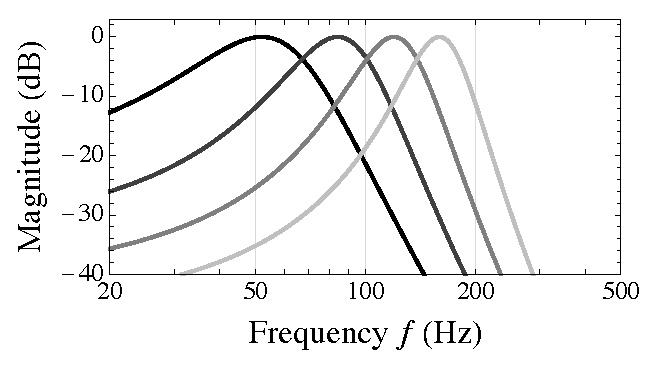
\includegraphics[width=\textwidth]{04_auditory_models/figures/gammatone_mag.eps}
        		\caption{Gammatone filters, $H_\Gamma$}
        		\label{fig:04_Auditory_Models:Gammatone_Filters}
    	\end{subfigure}
	\hfill
    	\begin{subfigure}[b]{0.49\textwidth}
        		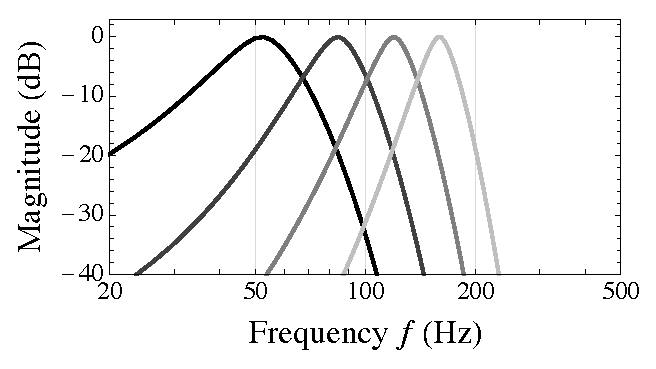
\includegraphics[width=\textwidth]{04_auditory_models/figures/patterson_mag.eps}
        		\caption{Patterson's filters, $H_\text{P}$}
        		\label{fig:04_Auditory_Models:Patterson_Filters}
    	\end{subfigure}
	
	\caption[Magnitude responses of gammatone filters and Patterson's filters.]{
	Magnitude responses of gammatone filters (left panel) and Patterson's filters (right) for the first four ERB-spaced center frequencies increasing from approximately 50~Hz.}
	\label{fig:04_Auditory_Models:Auditory_Filters}
\end{figure*}

We further define the level error given in dB by
\begin{equation}\label{eq:04_Auditory_Models:Audible_Energy_Difference}
e_\lambda = \tilde{\lambda} - \lambda,
\end{equation}
where $\lambda$ is the MAE for a reference signal and $\tilde{\lambda}$ is that for a test signal.

\section{Coloration metrics}\label{sec:04_Auditory_Models:Coloration_Metrics}
Generally, we use the term \textit{spectral coloration} to refer to any changes in the spectral content of a signal, for instance due to the application of a filter whose magnitude response is not constant.
However, as not all colorations are equally audible, metrics which mimic auditory filtering processes offer more perceptually-relevant estimates of colorations.
Here, we review five metrics that all aim to quantify such colorations.
For several of these metrics, we further define the \textit{spectral range}, given by
\begin{equation}\label{eq:Spectral_Range}
\rho_S = \max_c S(f_c) - \min_c S(f_c),
\end{equation}
and the \textit{spectral deviation}, given by
\begin{equation}\label{eq:Spectral_Deviation}
\sigma_S = \sqrt{\frac{1}{N_b} \sum_{c = 1}^{N_b} \left( S(f_c) - \overline{S} \right)^2},
\end{equation}
where $S$ is some metric (specified in dB, unless stated otherwise) and $\overline{S}$ is its average over all frequency bands.
For these metrics, we use the frequency range $f \in [f_\text{L}, f_\text{U}]$ with $f_\text{L} = 50$~Hz and $f_\text{U} = 21$~kHz, as recommended by~\citet{Boren2015}.

%% Scharer's ABSE
\subsection{Auditory band spectral error (\texorpdfstring{$\eta$}{eta})}\label{sec:04_Auditory_Models:Coloration_Metrics:ABSE}
The \textit{auditory band spectral error} (ABSE), adapted from \citet[Eq.~(9)]{ScharerLindau2009}, is given by
\begin{equation}\label{eq:ABSE}
\eta(f_c) = 10 \log_{10} \left( \frac{\int |H_\Gamma(f;f_c)| |\tilde{A}_0(f)|^2 df}{\int |H_\Gamma(f;f_c)| |A_0(f)|^2 df} \right),
\end{equation}
where $A_0$ and $\tilde{A}_0$ are the zeroth-order terms of the reference and test (respectively) ambisonics transfer functions and integration is taken over all frequencies.
For this and other coloration metrics requiring an auditory filter bank, we use ERB-spaced center frequencies \citep{GlasbergMoore1990} spanning the range $f \in [f_\text{L}, f_\text{U}]$ and denoted $f_c$ for $c \in [1, N_b]$.
In this case, we define the spectral range and deviation of the ABSE: $\rho_\eta, \sigma_\eta$, respectively.

 %% Boren's Epk and En
\subsection{Peak and notch errors (\texorpdfstring{$E_{\text{pk}}, E_\text{n}$}{Epk, En})}\label{sec:04_Auditory_Models:Coloration_Metrics:Epk}
The \textit{peak and notch errors} ($E_{\text{pk}}, E_\text{n}$) were defined by \citet{Boren2015}
and essentially quantify the average peak (or notch) height (depth) in a frequency response over a certain frequency range.
First, the difference (in dB) is computed between finely- and coarsely-smoothed versions of the the normalized free-field transfer function $\tilde{A}_0(f)/A_0(f)$, i.e.,
\begin{equation}
D(f) = 20 \log_{10} \left( \frac{ \mathcal{S}\left( \left| \tilde{A}_0(f)/A_0(f) \right| ; 1/48 \right) }{ \mathcal{S}\left( \left| \tilde{A}_0(f)/A_0(f) \right| ; 1 \right) } \right),
\end{equation}
where $\mathcal{S}(X; B)$ denotes fractional-octave smoothing applied to the spectrum $X$ with smoothing bandwidth $B$ octaves.
Here, we used the fractional-octave smoothing method of \citet{Tylka2017}, reproduced in \apxref{chap:A3_Smoothing_Weights}.

The peak- and notch-finding algorithms described by \citeauthor{Boren2015} are then applied to find the frequencies $f_1^\uparrow, f_2^\uparrow, \dots f_{N_\text{pk}}^\uparrow$ of all $N_\text{pk}$ spectral peaks and $f_1^\downarrow, f_2^\downarrow, \dots f_{N_\text{n}}^\downarrow$  of all $N_\text{n}$ spectral notches in the range $f \in [f_\text{L}, f_\text{U}]$.
The peak and notch errors are then given by \citep[Eq.~(1)]{Boren2015}
\begin{equation}
E_\text{pk} = \frac{\sum_{j = 1}^{N_\text{pk}} D(f_j^\uparrow)}{3 \log_2 (f_\text{U}/f_\text{L})}
\quad\quad\text{and}\quad\quad
E_\text{n} = \frac{\sum_{j = 1}^{N_\text{n}} (-D(f_j^\downarrow))}{3 \log_2 (f_\text{U}/f_\text{L})},
\end{equation}
respectively.
Note that, since $D$ is given in dB, the negative sign in the second equation typically ensures that both metrics are positive-valued.

%% Kates' CS
\subsection{Central spectrum (CS)}
The \textit{central spectrum} (CS) was defined by \citet{Kates1984} for use as a metric for comparing loudspeaker responses.
Consequently, it may be employed using only the free-field transfer functions of the test and reference signals.
Essentially, the metric is computed as the sum of the Fourier coefficients and critical band energies of a time-weighted autocorrelation of the input signal (see the original paper for details).
We then compute the difference (in dB) between the central spectra for the test and reference signals, given by
\begin{equation}
e_\text{CS}(f_c) = \widetilde{\text{CS}}(f_c) - \text{CS}(f_c).
\end{equation}
As done for the ABSE, we define the spectral range and deviation of the CS: $\rho_{e_\text{CS}}, \sigma_{e_\text{CS}}$, respectively.

%% Pulkki's CLL
\subsection{Composite loudness level (CLL)}\label{sec:04_Auditory_Models:Coloration_Metrics:Pulkki_CLL}
The \textit{composite loudness level} (CLL) spectrum was defined by \citet[section 1.1]{Pulkki1999} to give an estimate of perceived loudness.
Computing the CLL requires binaural impulse responses, which we compute using \eqnref{eq:02_Acoustical_Theory:PW_Quadrature_Binaural}.
The CLL spectrum is then computed as the sum of the two ears' loudness level spectra, each of which are given in phons%
\footnote{The \textit{phon} is a unit of perceived loudness, and is related to dB SPL via the equal-loudness contours originally described by \citet{FletcherMunson1933}.
Similar to dB, a change in perceived loudness is computed via a difference of values in phons.}
and found via a gammatone filter bank, half-wave rectification, low-pass filtering, and time-averaging of the signal energy in each band (see the original paper for details).
We then compute the difference (in phons) between the CLL spectra for the test and reference samples, given by
\begin{equation}\label{eq:04_Auditory_Models:Pulkki_CLL}
e_\text{CLL}(f_c) = \widetilde{\text{CLL}}(f_c) - \text{CLL}(f_c).
\end{equation}
We then define the spectral range and deviation of the CLL: $\rho_{e_\text{CLL}}, \sigma_{e_\text{CLL}}$, respectively.

%% Wittek's SA
\subsection{Internal spectrum (IS)}\label{sec:04_Auditory_Models:Coloration_Metrics:Wittek_IS}
\citet{Wittek2007} adapted the \textit{internal spectrum} (IS) defined by \citet[chapter 5]{Salomons1995PhD} in order to define so-called \textit{spectral alterations}.
These spectral alterations are computed as the difference (in dB) between the internal spectra for the test and reference signals, given by
\begin{equation}
e_\text{IS}(f_c) = \widetilde{\text{IS}}(f_c) - \text{IS}(f_c).
\end{equation}
According to \citet[section 3.2.5]{Wittek2007}, the IS for each signal is given as the average of the binaural power spectra, i.e.,
\begin{equation}
\text{IS}(f_c) = 10 \log_{10} \left( \frac{P^\text{L}(f_c) + P^\text{R}(f_c)}{2} \right).
\end{equation}
Here, $P^{\text{L},\text{R}}$ are the binaural power spectra after critical-band filtering, given by \citep[Eq.~(5.12)]{Salomons1995PhD}
\begin{equation}
P^{\text{L},\text{R}}(f_c) = \frac{\displaystyle \int_{-\infty}^\infty |H_\text{P}(f;f_c)| |\psi^{\text{L},\text{R}}(f)|^2 df}{\displaystyle \int_{-\infty}^\infty |H_\text{P}(f;f_c)| df},
\end{equation}
where $H_\text{P}(f;f_c)$ are Patterson's auditory filters (which are very similar in magnitude response to gammatone filters, as shown in \figref{fig:04_Auditory_Models:Auditory_Filters}) as specified by \citet[Eq.~(5.9)]{Salomons1995PhD} and $\psi^{\text{L},\text{R}}$ are the binaural transfer functions, given by the Fourier transform of the binaural impulse responses from \eqnref{eq:02_Acoustical_Theory:PW_Quadrature_Binaural}.
Again, we define the spectral range and deviation of the IS: $\rho_{e_\text{IS}}, \sigma_{e_\text{IS}}$, respectively.
Note that $\rho_{e_\text{IS}}$ is precisely equivalent to the $A_0$-measure defined by \citet[section 3.2.6]{Wittek2007}, which is based on the $A_0$-criterion defined by \citet[section 5.4]{Salomons1995PhD}.
Additionally, $\sigma_{e_\text{IS}}$ is essentially equivalent to the ``spectral deviation'' described by \citet[section 3.2.6]{Wittek2007}.

\section{Localization models}\label{sec:04_Auditory_Models:Localization_Models}
Generally, we use the term \textit{source localization} to refer to the perceived direction of a sound source relative to a listener.
Here, we review two well-established primitive localization vectors and describe two more sophisticated localization models.
For a predicted localization direction $\hat{\nu}$ (computed at the position of the listener), the localization error $e_\nu$ is given by
\begin{equation}\label{eq:04_Auditory_Models:Localization_Error}
e_\nu = \cos^{-1} \left( \hat{\nu} \cdot \hat{s}_0{}' \right),
\end{equation}
where $\hat{s}_0{}'$ is the direction of the source relative to the listener, found by normalizing the vector $\vec{s}_0{}' = \vec{s}_0 - \vec{r}_0$.

%% Gerzon's Localization Vectors
\subsection{Velocity and energy vectors (\texorpdfstring{$\vec{\nu}_{\text{V}}, \vec{\nu}_{\text{E}}$}{vV, vE})}\label{sec:04_Auditory_Models:Localization_Vectors}
To predict the localization of sound in multichannel playback systems, \citet{Gerzon1992} defines two localization metrics: the velocity and energy vectors.
Note that these definitions assume that the loudspeakers are equidistant from the listening position, such that the signals all arrive coincidentally.

The velocity vector is used to predict localization due to interaural time differences at low frequencies ($<700$~Hz) and is given by \citep{Gerzon1992}
\begin{equation}\label{eq:04_Auditory_Models:Velocity_Vector}
\vec{\nu}_{\text{V}}(f) = \textrm{Re} \left\{ \frac{ \sum_q G_q(f) \hat{v}_q}{ \sum_q G_q(f)} \right\},
\end{equation}
where $\text{Re} \left\{ \cdot \right\}$ denotes taking the real part of the argument, $G_q$ is the complex-valued, frequency-dependent ``gain'' of the $q^{\text{th}}$ source, and $\vec{v}_q$ is the position of that source.
The energy vector is used to predict localization due to interaural level differences at higher frequencies (500~Hz -- 5~kHz) and is given by \citep{Gerzon1992}
\begin{equation}\label{eq:04_Auditory_Models:Energy_Vector}
\vec{\nu}_{\text{E}}(f) = \frac{ \sum_q |G_q(f)|^2 \hat{v}_q}{ \sum_q |G_q(f)|^2}.
\end{equation}
The directions of these vectors indicate the expected localization direction and their magnitudes indicate the quality of the localization.
Ideally, the vectors should have a magnitude equal to unity and point in the direction of the virtual source.

%% Stitt's Localization Model
\subsection{Precedence-effect-based energy vector (\texorpdfstring{$\vec{\nu}_{\text{PE}}$}{vPE})}\label{sec:04_Auditory_Models:PE_Energy_Vector}
Recently, \citet{Stitt2016} proposed an extension to incorporate the precedence effect into the energy vector of \citet{Gerzon1992}.
In their paper, \citeauthor{Stitt2016} also showed that their proposed model achieves improved localization prediction accuracy compared to the binaural models of \citet{Dietz2011} and \citet{Lindemann1986a}.
The model predicts localization by computing a weighted average of position vectors for each of a finite set of point sources.
The model assumes that each source is generating the same signal, although perhaps at different amplitudes, and perhaps with different distances between each source and the listener.
Perceptual weights are first computed for each source based its time-of-arrival to and amplitude at the listening position.
The calculation of these weights is not trivial, but briefly, it involves weighting earlier signals more heavily, but adjusting the weights of later signals based on their amplitudes and directions-of-arrival (see the original paper for details).

The predicted localization is then given as a vector by
\begin{equation}\label{eq:PE_Energy_Vector}
\vec{\nu}_{\text{PE}} = \frac{ \displaystyle \sum_{q=1}^Q |w_q(\alpha) G_q / v_q|^2 \, \hat{v}_q}{ \displaystyle \sum_{q=1}^Q |w_q(\alpha) G_q / v_q|^2},
\end{equation}
where $w_q$ is the perceptual weight for the $q^\text{th}$ source, $G_q$ is the amplitude of the $q^\text{th}$ source, $v_q$ is the distance of the $q^\text{th}$ source, $\hat{v}_q$ is a unit vector pointing towards the $q^\text{th}$ source, and $\alpha \in [0,1]$ is a free parameter which specifies the relative importance of stationary (i.e., time-averaged) to transient information in the stimulus signal.%
\footnote{For example, a highly transient signal is expected to require a low value of $\alpha$, while a more stationary signal would require a higher value \citep{Stitt2016,Stitt2017}.}

%% Dietz' Model
\subsection{Binaural localization model (\texorpdfstring{$\vec{\nu}_{\text{B}}$}{vB})}\label{sec:04_Auditory_Models:Binaural_Localization_Model}
We also consider the binaural localization model of \citet{Dietz2011}.
In order to compute the required binaural impulse responses, the ambisonics impulse response is first converted to plane-wave impulse responses using \eqnref{eq:02_Acoustical_Theory:A2mu}.
The binaural impulse responses are then computed by \eqnref{eq:02_Acoustical_Theory:PW_Quadrature_Binaural}.

An implementation of this model is freely available in the auditory modeling toolbox,\citefooturl{AMTURL} authored by \citet{SondergaardMajdak2013}.
The core of the model \citep{Dietz2011} emulates inner-ear processes (e.g., auditory band filtering, signal compression, half-wave rectification, etc.) in order to compute binaural parameters such as the interaural time difference (ITD), interaural level difference, and interaural coherence in a range of frequency bands for both the envelope and fine-structure components of the binaural signals (see the original paper for details).
In this work, we adopted the extension proposed by \citet{Wierstorf2013}, in which an ITD-to-azimuth lookup table is first generated for each subject using that subject's measured HRTFs on the frontal horizontal plane.
The stimulus signal is then filtered by the binaural impulse responses and the ITD is computed using the original model.
The model yields ITD in a set of frequency bands, which are then converted to azimuth via the lookup table.
Outliers beyond $30^\circ$ away from the median azimuth are then removed, and finally, a single predicted azimuth, $\phi_{\text{B}}$, is computed as the weighted average over frequency, with weights given by the rms signal amplitude in each frequency band.
The predicted localization direction is then given by
\begin{equation}
\vec{\nu}_{\text{B}} = (\cos \phi_{\text{B}}, \sin \phi_{\text{B}}, 0).
\end{equation}

\section{Physical metrics}\label{sec:04_Auditory_Models:Physical_Metrics}
Here, we describe physical metrics for the acoustic intensity vector and diffuseness.
According to \citet{MerimaaPulkki2005}, the acoustic intensity vector and a diffuseness parameter can be computed using the four standard ``B-format'' signals.
These signals are related to the first four ACN/N3D ambisonics signals by
\begin{equation}
\begin{split}
W &= A_0 / \sqrt{2}, \\
Y &= A_1 / \sqrt{3}, \\
Z &= A_2 / \sqrt{3}, \\
X &= A_3 / \sqrt{3},
\end{split}
\end{equation}
where this relationship can be derived by comparing \eqnref{eq:02_Acoustical_Theory:PlaneSource_An} and the B-format encoding equations specified by \citet[p.~62]{MalhamMyatt1995}.
We now construct a frequency-dependent Cartesian row vector, $\vec{X}$, given by
\begin{equation}
\vec{X} \equiv \begin{bmatrix} X & Y & Z \end{bmatrix} = \frac{1}{\sqrt{3}} \begin{bmatrix} A_3 & A_1 & A_2 \end{bmatrix} = \frac{\vec{A}}{\sqrt{3}},
\end{equation}
where we have further defined a proportional vector $\vec{A} = \left[ A_3, A_1, A_2 \right] = \sqrt{3} \vec{X}$.
We will also need the acoustic impedance of the medium, $Z_0 = \rho_0 c$, where $\rho_0 \approx 1.225$~kg/m\textsuperscript{3} is the density of the medium and $c \approx 343$~m/s is the speed of sound.

\subsection{Acoustic intensity vector (\texorpdfstring{$\vec{\nu}_{\text{I}}$}{vI})}\label{sec:04_Auditory_Models:Intensity_Vector}
Using the above, the acoustic intensity vector, $\vec{\nu}_{\textrm{I}}$, is given by \citep[Eq.~(11)]{MerimaaPulkki2005}
\begin{equation}\label{eq:04_Auditory_Models:Intensity_Vector}
\vec{\nu}_{\textrm{I}}(f) = \frac{\sqrt{2}}{Z_0} \text{Re} \left\{ \overline{W}(f) \vec{X}(f) \right\} = \frac{1}{{Z_0 \sqrt{3}}} \text{Re} \left\{ \overline{A_0}(f) \vec{A}(f) \right\},
\end{equation}
where $\overline{(\cdot)}$ and $\text{Re} \left\{ \cdot \right\}$ denote taking the complex conjugate and the real part of the argument, respectively.

\subsection{Diffuseness parameter (\texorpdfstring{$\Psi$}{Psi})}\label{sec:04_Auditory_Models:Diffuseness_Parameter}
Additionally, the diffuseness parameter $\Psi$ is given by \citep[Eq.~(12)]{MerimaaPulkki2005}
\begin{equation}\label{eq:04_Auditory_Models:Diffuseness}
\begin{split}
\Psi(f) &= 1 - \sqrt{2} \frac{ \left\| \text{Re} \left\{ \overline{W}(f) \vec{X}(f) \right\} \right\|}{\left| W(f) \right|^2 + \left\| \vec{X}(f) \right\|^2 / 2} \\
	&= 1 - \frac{2}{\sqrt{3}} \frac{ \left\| \text{Re} \left\{ \overline{A_0}(f) \vec{A}(f) \right\} \right\|}{\left| A_0(f) \right|^2 + \left\| \vec{A}(f) \right\|^2 / 3}
\end{split}
\end{equation}
where $\left\| \cdot \right\|$ denotes the norm of a complex-valued vector, given by
\begin{equation}
\| \vec{x} \| = \sqrt{\left\langle \vec{x}, \vec{x} \right\rangle} \equiv \sqrt{\vec{x} \vec{x}^\text{H}},
\end{equation}
where $(\cdot)^\text{H}$ denotes the conjugate (Hermitian) transpose of the argument.
We then compute the logarithmically-weighted mean of the difference between the diffuseness spectra for the test and reference samples, given by
\begin{equation}
e_\Psi = \frac{\displaystyle \int_{f_\text{L}}^{f_\text{U}} \frac{1}{f} \left( \tilde{\Psi}(f) - \Psi(f) \right) df}{\log(f_\text{U}) - \log(f_\text{L})},
\end{equation}
where $f_\text{L} = 50$~Hz and $f_\text{U} = 21$~kHz.

\section{Summary of metrics and models}
In this thesis, we consider only one metric for sound level (see \eqnref{eq:04_Auditory_Models:Mean_Audible_Energy}) and one metric for diffuseness (\eqnref{eq:04_Auditory_Models:Diffuseness}).
For coloration and localization, however, we have a variety of metrics and models to choose from.
In this section, we summarize the main equations for, and important differences between, the coloration metrics and localization models reviewed in this chapter.

\subsection{Coloration metrics}
As defined in \secref{sec:04_Auditory_Models:Coloration_Metrics}, the auditory band spectral error (ABSE), the peak and notch errors, and the central spectrum all take monaural input signals, for which we use the omnidirectional term of the ambisonics input signals.
The composite loudness level and the internal spectrum, however, take binaural input signals, which therefore require first rendering the ambisonics input signals to binaural using one of the methods described in \secref{sec:02_Acoustical_Theory:Binaural_Rendering}.

\begin{table}[tbp]
\centering
\begin{tabular}{c|c|c}
\textbf{Metric} & \textbf{Equation(s)} & \textbf{Input} \\\hline\hline
\rule[-0.8cm]{0pt}{1.7cm} \parbox{4cm}{\centering Auditory band spectral error} & $\eta(f_c) = 10 \log_{10} \displaystyle \left( \frac{\int |H_\Gamma(f;f_c)| |\tilde{A}_0(f)|^2 df}{\int |H_\Gamma(f;f_c)| |A_0(f)|^2 df} \right)$ & Monaural \\\hline
\rule[-0.8cm]{0pt}{1.7cm} Peak error & $E_\text{pk} = \displaystyle \frac{\sum_{j = 1}^{N_\text{pk}} D(f_j^\uparrow)}{3 \log_2 (f_\text{U}/f_\text{L})}$ & Monaural \\\hline
\rule[-0.8cm]{0pt}{1.7cm} Notch error & $E_\text{n} = \displaystyle \frac{\sum_{j = 1}^{N_\text{n}} (-D(f_j^\downarrow))}{3 \log_2 (f_\text{U}/f_\text{L})}$ & Monaural \\\hline
\rule[-0.5cm]{0pt}{1.1cm} Central spectrum & $e_\text{CS}(f_c) = \widetilde{\text{CS}}(f_c) - \text{CS}(f_c)$ & Monaural \\\hline
\rule[-0.6cm]{0pt}{1.3cm} \parbox{4cm}{\centering Composite loudness level} & $e_\text{CLL}(f_c) = \widetilde{\text{CLL}}(f_c) - \text{CLL}(f_c)$ & Binaural \\\hline
\rule[-1.5cm]{0pt}{3.1cm} Internal spectrum & 
  \begin{tabular}{c}
  $\text{IS}(f_c) = 10 \log_{10} \displaystyle \left( \frac{P^\text{L}(f_c) + P^\text{R}(f_c)}{2} \right)$ \\[0.5cm]
  $e_\text{IS}(f_c) = \widetilde{\text{IS}}(f_c) - \text{IS}(f_c)$
  \end{tabular} & Binaural
\end{tabular}
\caption[Summary of main equations for coloration metrics.]{
Summary of main equations for the coloration metrics reviewed in \secref{sec:04_Auditory_Models:Coloration_Metrics}.
The third column indicates the type of input signal needed for the metric, where ``monaural'' indicates that the metric requires only the omnidirectional ambisonics signal as the input.}
\label{tab:04_Auditory_Models:Coloration_Equations}
\end{table}

Additionally, only the ABSE and the peak and notch errors were originally defined as relative measures of coloration, since a comparison between the test and reference samples is ``built-in'' to the equations for each metric.
The other metrics were instead originally defined as absolute measures of the perceived spectrum, so, for each of these metrics, we have had to define an additional relative measure, in the form of a difference between test and reference spectra.

The main equations describing these metrics are reproduced in \tabref{tab:04_Auditory_Models:Coloration_Equations}.
Recall that for all of the metrics except the peak and notch errors, we eliminate the frequency-dependence by subsequently computing the spectral range and deviation (see \eqnreftwo{eq:Spectral_Range}{eq:Spectral_Deviation}) of each error spectrum.
The perceptual relevance of these various coloration metrics will be evaluated via subjective testing in \chapref{chap:05_Proposed_Models}

\subsection{Localization models}
As defined in \secref{sec:04_Auditory_Models:Localization_Models}, the velocity, energy, and precedence-effect-based localization vectors all take as inputs discrete source gains and positions.
Consequently, none of those vectors can be used to predict localization directly from ambisonics signals; only the binaural localization model uses actual input signals in order to predict perceived localization.
The main equations describing these models are reproduced in \tabref{tab:04_Auditory_Models:Localization_Equations}.

\begin{table}[tbp]
\centering
\begin{tabular}{c|c|c}
\textbf{Metric} & \textbf{Equation(s)} & \textbf{Input} \\\hline\hline
\rule[-0.8cm]{0pt}{1.7cm} Velocity vector & $\vec{\nu}_{\text{V}}(f) = \textrm{Re} \left\{ \displaystyle \frac{ \sum_q G_q(f) \hat{v}_q}{ \sum_q G_q(f)} \right\}$ & Source gains \\\hline
\rule[-0.8cm]{0pt}{1.7cm} Energy vector & $\vec{\nu}_{\text{E}}(f) = \displaystyle \frac{ \sum_q |G_q(f)|^2 \hat{v}_q}{ \sum_q |G_q(f)|^2}$ & Source gains \\\hline
\rule[-1.5cm]{0pt}{3.1cm} \parbox{5cm}{\centering Precedence-effect-based energy vector} & $\vec{\nu}_{\text{PE}} = \displaystyle \frac{ \displaystyle \sum_{q=1}^Q |w_q(\alpha) G_q / v_q|^2 \, \hat{v}_q}{ \displaystyle \sum_{q=1}^Q |w_q(\alpha) G_q / v_q|^2}$ & Source gains \\\hline
\rule[-0.8cm]{0pt}{1.7cm} \parbox{5cm}{\centering Binaural localization model} & $\vec{\nu}_{\text{B}} = (\cos \phi_{\text{B}}, \sin \phi_{\text{B}}, 0)$ & Binaural \\\hline
\rule[-0.8cm]{0pt}{1.7cm} Intensity vector & $\vec{\nu}_{\textrm{I}}(f) = \displaystyle \frac{\sqrt{2}}{Z_0} \text{Re} \left\{ \overline{W}(f) \vec{X}(f) \right\}$ & Ambisonics
\end{tabular}
\caption[Summary of main equations for localization models.]{
Summary of main equations for the localization models reviewed in \secreftwo{sec:04_Auditory_Models:Localization_Models}{sec:04_Auditory_Models:Physical_Metrics}.
The third column indicates the type of input signals needed for the model.}
\label{tab:04_Auditory_Models:Localization_Equations}
\end{table}

%\rule[-0.8cm]{0pt}{1.7cm}

It is worth noting that the acoustic intensity vector, as defined in \secref{sec:04_Auditory_Models:Physical_Metrics}, does take ambisonics signals as inputs.
However, as this is a purely physical metric, it does not necessarily correspond to the localization of a source as perceived by a human listener.
Similarly, although the velocity and energy vectors can be indicative of perceived localization, they neglect many relevant psychoacoustic phenomena (e.g., the precedence effect) and processes of the human auditory system (as a result, they are often described as localization ``primitives,'' rather than localization models), so they should not be expected to give accurate predictions of perceived localization.

In \chapref{chap:05_Proposed_Models}, we present an extension to the precedence-effect-based energy vector in order to use ambisonics signals as inputs to the model.
In that chapter, we also compare our proposed extension to the binaural localization model in terms of their agreement with subjective test data.
%%%% PROPOSED MODELS %%%%
\chapter{Auditory models for evaluating navigational methods}\label{chap:05_Proposed_Models}
In this chapter, we propose and validate models that predict perceived source localization (i.e., the direction of a source relative to the listener) and spectral coloration (changes in the spectral content of a sound) for the specific purpose of evaluating navigational methods for ambisonics-encoded sound fields.
Previous evaluations of navigational methods have typically relied on binaural localization models, which conflate the effects of the navigational method with those of the adopted ambisonics-to-binaural rendering approach, and previous studies on navigation-induced coloration have been largely qualitative.
Consequently, in this chapter, we seek to develop perceptually-relevant auditory models that can be applied directly to translated ambisonics impulse responses (i.e., before rendering to binaural) and give numerical predictions for localization direction and coloration.

\section{Introduction}\label{sec:05_Proposed_Models:Introduction}
Of the several navigational methods reviewed in \chapref{chap:03_Navigation_Techniques}, we expect that they all may degrade localization information and induce spectral coloration, leading to errors in the perceived directions of sound sources and audible changes in the spectral content of the signals, respectively.
The severity of such penalties needs to be investigated and quantified in order to both compare existing navigational methods and develop novel ones.
Although subjective testing is the most direct method of evaluating and comparing navigational methods, such tests are often lengthy and costly, which motivates the use of objective metrics that enable quick assessments of navigational methods.

% Review of previous work focusing on the remaining problems (questions or deficiencies) the present paper claims to contribute to solving
\subsection{Previous work and remaining problems}
Several recent studies have investigated the localization accuracy of various navigational methods.
\citet{Winter2014} evaluated the localization accuracy of the plane-wave-based translation method of \citet{SchultzSpors2013} (reviewed in \secref{sec:03_Navigation_Techniques:PW_Technique}) using the binaural localization model of \citet{Dietz2011} (reviewed in \secref{sec:04_Auditory_Models:Binaural_Localization_Model}) to predict perceived localization.
\citet{TylkaChoueiri2015} compared the localization errors incurred by three extrapolation-based translation methods (reviewed in \secref{sec:03_Navigation_Techniques:Extrapolation_Methods}) using the velocity and energy localization vectors developed by \citet{Gerzon1992} (reviewed in \secref{sec:04_Auditory_Models:Localization_Vectors}).
However, this analysis neglected the precedence effect, which is expected to play an important role in the context of sound field navigation, as an accurate virtual translation of the listener necessarily involves direction-dependent time shifting of incident signals.
Consequently, more recently, \citet{TylkaChoueiri2016} evaluated the localization accuracy of their proposed interpolation-based navigational method (introduced here in \chapref{chap:08_Proposed_Method}) using an extension of a precedence-effect-based localization vector developed by \citet{Stitt2016} (reviewed in \secref{sec:04_Auditory_Models:PE_Energy_Vector}), which was itself an extension of Gerzon's original energy vector.
Although the model of \citeauthor{Stitt2016} has been validated through listening tests and shows improvements compared to binaural localization models (specifically, those by \citet{Dietz2011} and \citet{Lindemann1986a}) the more recent extension by \citet{TylkaChoueiri2016} had not, at the time of publication, been validated through listening tests.

Additionally, recent studies have investigated spectral colorations induced by various navigational methods.
\citet{HahnSpors2015b} evaluated spectral coloration induced by the plane-wave translation method \citep{SchultzSpors2013} by visually examining impulse and frequency responses.
In a similar manner, \citet{TylkaChoueiri2016} evaluated and compared the spectral coloration induced by both their proposed interpolation method and the linear interpolation method of \citet{Southern2009} (reviewed in \secref{sec:03_Navigation_Techniques:XF_Technique}).
While it is clear from these studies that most (if not all) existing navigational methods tend to induce at least some spectral coloration, both analyses were largely qualitative.
Consequently, it remains difficult to compare these colorations between methods without numerical measures of perceptible coloration.

% A statement of the paper's main question(s) and goal(s), followed by a succinct description of the general method and approach to be described in the paper
\subsection{Objectives and approach}
In this chapter, we present models for perceived source localization and spectral coloration which we have developed for the purpose of evaluating and comparing methods for virtual navigation of ambisonics-encoded sound fields.
In order to isolate any errors introduced by the navigational method under test (which operates in the ambisonics domain) from those introduced through rendering to binaural, we developed models that are independent of any choice of ambisonics-to-binaural rendering approach (several of which are reviewed in \secref{sec:02_Acoustical_Theory:Binaural_Rendering}) since they operate directly on ambisonics impulse responses.
In contrast, although not explicitly investigated here, we expect the predictions of binaural models to be sensitive to the choice of binaural rendering approach and/or to the choice of head-related transfer function (HRTF).

For these models to be of any practical use, they must also be perceptually relevant, in that the predictions of the models should agree with subjective listening test responses.
Consequently, we conducted two listening experiments (one each for localization and coloration), the results of which were used to determine parameters of the proposed models.
We then validated the proposed models through comparisons against alternative models in terms of their agreement with the experimental data.

% A brief section by section description of the structure of the paper
In \secreftwo{sec:05_Proposed_Models:Localization_Model}{sec:05_Proposed_Models:Coloration_Models}, we describe the proposed localization and coloration models, respectively.
Then, in \secref{sec:05_Proposed_Models:Listening_Tests}, we describe the listening experiments conducted to validate the proposed models.
In \secref{sec:05_Proposed_Models:Results}, we compare the results of the listening experiments with predictions of the models, and finally, in \secref{sec:05_Proposed_Models:Conclusions}, we draw conclusions based on these results.

%%%% Auditory Models %%%%
%% Proposed Localization Model
\section{Localization model}\label{sec:05_Proposed_Models:Localization_Model}
Recently, \citet{Stitt2016} proposed an extension to incorporate the precedence effect into the energy vector of \citet{Gerzon1992}.
In their paper, \citeauthor{Stitt2016} also showed that their proposed model achieves improved localization prediction accuracy compared to the binaural models of \citet{Dietz2011} and \citet{Lindemann1986a}.
Motivated by these results, we proposed in a recent paper \citep{TylkaChoueiri2016} an extension to this localization model; here, we describe and revise our proposed extension.

We begin by converting the ambisonics impulse response into a set of $Q$ impulse responses for a specified grid of plane-wave directions, $\hat{v}_q$, with $q \in [1,Q]$.
For ambisonics order $L$, there are $N = (L + 1)^2$ ambisonics signals, $a_n(t)$, with $n \in [0, N-1]$, and the corresponding plane-wave signals, $\mu$, are given by \eqnref{eq:02_Acoustical_Theory:A2mu}.%
\footnote{Alternatively, this plane-wave decomposition could be computed using a pseudoinversion approach, as described in \eqnref{eq:02_Acoustical_Theory:A2mu_Pinv}, or a compressed sensing approach, as described by \citet[Eq.~(10)]{Epain2009}.}
The grids of directions (also called ``nodes'') used here are given by \citet{FliegeMaier1999}; these grids and their corresponding quadrature weights are freely available online.\citefooturl{FliegeNodesURL}
As this discrete plane-wave sound field would generally be rendered via quadrature integration (see \eqnref{eq:02_Acoustical_Theory:PW_Quadrature_Rendered_Field}), the impulse response for each plane-wave term is given by $g_q(t) = w_q \mu(t,\hat{v}_q)$, where $w_q$ is the quadrature weight for the direction $\hat{v}_q$.

Next, we identify and isolate temporally-distinct impulse response ``wavelets.''
To do this, we apply a $4^\textrm{th}$-order Butterworth high-pass filter with a cut-off frequency of 500~Hz to all impulse responses in the set and compute the global maximum (i.e., the largest absolute value over all impulse responses in the set).
For each impulse response, we take the absolute value and identify any peaks (i.e., local maxima) whose amplitudes are at least $G_\text{min}$~dB relative to the global maximum ($G_\text{min} \leq 0$~dB).
If no such peaks exist in a given impulse response, then that response in its entirety is treated as a wavelet.
If at least one such peak exists, then, around each peak, we apply a Tukey window beginning $\tau_\text{w}$~ms before the peak and ending either $\tau_\text{w}$~ms after the peak, or at the position of the following peak, whichever yields a larger window length.
Both the cosine fade-in and fade-out of the Tukey window are $\tau_\text{w}$~ms in duration.
In this way, a single impulse response may be split into several wavelets.%
\footnote{A simpler implementation of this stage of the model might follow a more traditional, uniformly-partitioned STFT approach, but we do not explore this idea here.}
For each wavelet, we apply a 10\% ($-20$~dB, now relative to the peak of that particular wavelet) threshold to determine the time-delay of the onset.

For the purposes of this model, we consider each wavelet to be a distinct sound source, such that wavelets extracted from the same impulse response originate from the same direction, but arrive at different times, given by their onset times.
Taking the Fourier transform of each wavelet yields complex-valued, frequency-dependent gains, $G_{q'}$, of the $q'{}^\text{th}$ wavelet, where $q' \in [1,Q']$ and $Q' \geq Q$ is the total number of wavelets.
We then average these gains in critical bands using a gammatone filter bank (see \figref{fig:04_Auditory_Models:Gammatone_Filters}),
such that the frequency-averaged gains are given by
\begin{equation}\label{eq:05_Proposed_Models:Localization_Model:FreqAvg_Gain}
\overline{G}_{q'}(f_c) = \frac{\displaystyle \int_{-\infty}^\infty |H_\Gamma(f;f_c)| |G_{q'}(f)| df}{\displaystyle \int_{-\infty}^\infty |H_\Gamma(f;f_c)| df},
\end{equation}
where the gammatone filters are taken for a set of ERB-spaced center frequencies spanning the range $f \in [20~\text{Hz}, 20~\text{kHz}]$.

For each frequency band, we feed these gains into the model, yielding a frequency-dependent predicted localization vector $\vec{\nu}_\textrm{PE}(f_c)$, given by
\begin{equation}\label{eq:05_Proposed_Models:PE_Energy_Vector}
\vec{\nu}_{\textrm{PE}}(f_c) = \frac{ \sum_{q'} |w_{q'}(\alpha) \overline{G}_{q'}(f_c)|^2 \, \hat{v}_{q'}}{ \sum_{q'} |w_{q'}(\alpha) \overline{G}_{q'}(f_c)|^2},
\end{equation}
where $\alpha$ is a parameter of the original model of \citet{Stitt2016} (discussed in \secref{sec:04_Auditory_Models:PE_Energy_Vector}) and $w_{q'}(\alpha)$ is a perceptual weight (based on the precedence-effect) for the $q'{}^\text{th}$ wavelet.
Similarly, we define a perceptually-weighted velocity vector, given by
\begin{equation}\label{eq:PE_Velocity_Vector}
\vec{\nu}_{\textrm{PV}}(f_c) = \text{Re} \left[ \frac{ \sum_{q'} w_{q'}(\alpha) \overline{G}_{q'}(f_c) \, \hat{v}_{q'}}{ \sum_{q'} w_{q'}(\alpha) \overline{G}_{q'}(f_c)} \right],
\end{equation}
where $\text{Re}(\cdot)$ denotes taking the real part of the argument.
Note that we include this step of ``taking the real part'' in our definition only to maintain consistency with the original definition of the velocity vector, given by \citet[section 4]{Gerzon1992}, in which complex-valued gains are used (see \eqnref{eq:04_Auditory_Models:Velocity_Vector}).
However, in our case, all $\overline{G}_{q'}$ are already real-valued (see \eqnref{eq:05_Proposed_Models:Localization_Model:FreqAvg_Gain}), so taking the real part has no effect on the result.
This deviation from the original definition may be justified since the time-dependence of the sources is now captured in the precedence-effect-based weights, so each source's phase is no longer needed.

We then combine the velocity vector below 700~Hz and the energy vector above into a single, frequency-dependent vector, given by
\begin{equation}
\vec{\nu}_{\textrm{PC}}(f_c) =
\begin{cases}
\displaystyle \frac{\left\| \vec{\nu}_{\textrm{PE}}(f_\text{XO}) \right\|}{\left\| \vec{\nu}_{\textrm{PV}}(f_\text{XO}) \right\|} \cdot \vec{\nu}_{\textrm{PV}}(f_c), & \text{for}~f_c \leq f_\text{XO}, \\
\vec{\nu}_{\textrm{PE}}(f_c), & \text{for}~f_c > f_\text{XO},
\end{cases}
\end{equation}
where $\|\cdot\|$ denotes the $\ell^2$ norm (Euclidean distance) of a vector, $f_\text{XO}$ is the ``crossover'' frequency, equal to the center frequency nearest to 700~Hz, and we have introduced a normalization factor to match low- and high-frequency vector magnitudes.
Finally, we compute a weighted-average vector, which depends on the stimulus signal and is given by
\begin{equation}
\vec{\nu}_{\textrm{P}} = \frac{\sum_c \overline{X}(f_c)\, \vec{\nu}_{\textrm{PC}}(f_c)}{\sum_c \overline{X}(f_c)},
\end{equation}
where the weights $\overline{X}(f_c)$ are the stimulus signal's energy in each critical band, given by
\begin{equation}
\overline{X}(f_c) = \frac{\displaystyle \int_{-\infty}^\infty |H_\Gamma(f;f_c)| |X(f)|^2 df}{\displaystyle \int_{-\infty}^\infty |H_\Gamma(f;f_c)| df},
\end{equation}
and $X(f)$ is the Fourier transform of the stimulus signal.

In addition to the three free model parameters ($Q$, $\tau_\text{w}$, and $G_\text{min}$) defined above, the original model of \citet{Stitt2016} retains one free parameter, $\alpha \in [0,1]$, which specifies the relative importance of stationary (i.e., time-averaged) to transient information in the stimulus signal (see \secref{sec:04_Auditory_Models:PE_Energy_Vector}).
As will be described below in \secref{sec:05_Proposed_Models:Localization_Results}, we determined optimal values for these four parameters based on a best fit of the model's predictions to the data from the listening experiment.

%% Proposed Coloration Models
\section{Coloration models}\label{sec:05_Proposed_Models:Coloration_Models}
In this work, we followed the approach of \citet{Wittek2007} and developed linear regression models to predict subjective ratings of coloration given some combination of the coloration metrics reviewed in \secref{sec:04_Auditory_Models:Coloration_Metrics}.
As discussed in \chapref{chap:04_Auditory_Models}, we define each of these metrics \textit{relative} to some reference signal.
Consequently, each metric is computed using both a \textit{test sample} (i.e., the ambisonics impulse response for the listening position after processing through some navigational method) and a \textit{reference sample} (i.e., the ambisonics impulse response captured directly at the listening position).

In this work, we used the combinations of coloration metrics listed in \tabref{tab:Coloration_Models} to create multiple linear regression models, each of which predicts subjective ratings of coloration.
Regression coefficients were found by fitting the predictions of each model to the data, as will be discussed below in \secref{sec:05_Proposed_Models:Coloration_Results}.

% Table of coloration models and corresponding metrics
\begin{table}[t]
\centering
 \begin{tabular}{|c|c|} \hline
 \textbf{Model Name} & \textbf{Metrics Used} \\ \hline
 Proposed & $\rho_\eta, \sigma_\eta, E_\text{pk}, E_\text{n}$ \\
 \citet{Kates1984} & $\rho_{e_\text{CS}}, \sigma_{e_\text{CS}}$ \\
 \citet{Pulkki1999} & $\rho_{e_\text{CLL}}, \sigma_{e_\text{CLL}}$ \\
 \citet{Wittek2007} & $\rho_{e_\text{IS}}, \sigma_{e_\text{IS}}$ \\ \hline
 \end{tabular}
 \caption{Metrics used for each coloration model.}
 \label{tab:Coloration_Models}
\end{table}

%%%% Validation of Proposed Models %%%%
\section{Listening experiments}\label{sec:05_Proposed_Models:Listening_Tests}
Two listening experiments were conducted in an acoustically-treated listening room,
where the listener was seated and given a pair of headphones.
Four subjects, all male, ages 25--30 years, participated in the experiments;
each subject is an experienced audio engineer or researcher.
Prior to the experiments, each subject's HRTFs were measured in an anechoic chamber.
These HRTFs were measured also as part of an ongoing project to compile a database of measured HRTFs \citep{Sridhar2017}.
The procedures employed to collect and process these measurements are reproduced in \apxref{chap:A4_HRTF_Measurements}.

Each subject's HRTFs were used to generate an individualized ambisonics-to-binaural rendering configuration for the ambiX binaural decoder plug-in \citep{Kronlachner2013,ambiXPlugInURL}.
In this decoder, we performed a basic (pseudoinverse) ambisonic decoding (see \eqnref{eq:02_Acoustical_Theory:PinvDecoder}) for a 36-node Fliege grid and filtered each virtual loudspeaker's signal by the nearest measured HRTF.
This decoder was generated using an early version of the SOFA/ambiX binaural rendering (SABRE) toolkit, which was developed by the present author and is described in \apxref{chap:A2_SABRE_Toolkit}.
The headphones (Stax SR-009) were equalized for each subject using a regularized, least-squares equalization filter \citep{ScharerLindau2009}.

The test samples were produced using the weighted average method and a regularized least-squares interpolation method (described in \secreftwo{sec:03_Navigation_Techniques:XF_Technique}{sec:08_Proposed_Method:Reg-LS_Technique}, respectively), employed for microphone spacings of 10, 30, or 50~cm.
The test samples were rendered from 4\textsuperscript{th}-order ambisonics room impulse responses for microphone positions distributed on both sides of the listening position, as illustrated by the empty circles in \figref{fig:Test_Geometry}.
For the localization test, these impulse responses were measured with a 32-capsule spherical microphone array, using phase-controlled exponential sine sweeps and an exact deconvolution of the recorded signals by the input signal, as described in \apxref{chap:A5_Impulse_Response}.
For the coloration test, on the other hand, the impulse responses were simulated using a MATLAB-based room acoustics simulator%
\footnote{In this work, we used the Multichannel Room Acoustics Simulator (\textsc{MCRoomSim}) package \citep{Wabnitz2010,MCRoomSimURL}.}
with a room model similar in size and acoustics to the actual listening room.
Also included in each test were reference samples, measured at the listening position and for which no interpolation was performed.
All stimuli were presented at levels between 60~dB and 78~dB (A-weighted), $\pm4$~dB.

% Diagram of source/mic positions
\begin{figure}[t]
\centering
  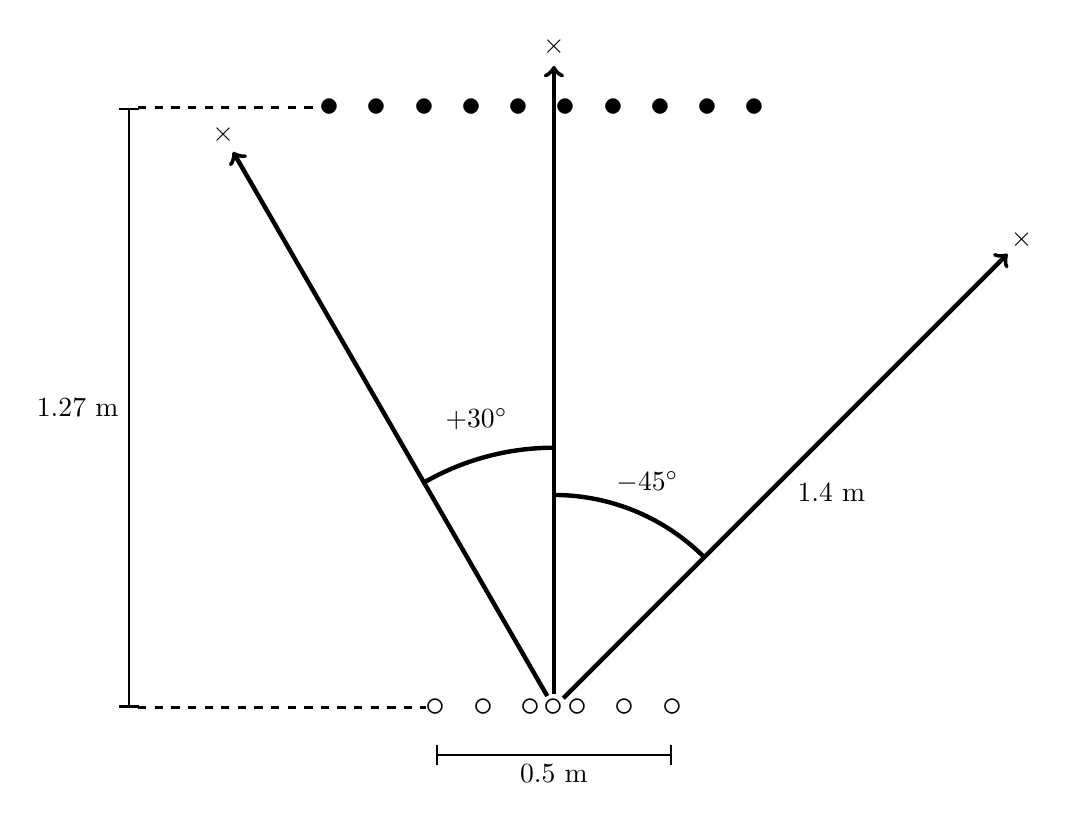
\begin{tikzpicture}[scale=6]
% Parameters
\def\radius{1.4};
\def\arrowStart{0.02};
\def\arrowScale{0.97};
\def\arcRadius{0.5};
\def\micSpacing{0.1};
\def\spkrSpacing{0.05};
\def\spkrDistance{1.27};
\def\offset{0.02};
\pgfmathsetmacro\colLefty{cos(-30)*\radius}
\pgfmathsetmacro\colLeftx{sin(-30)*\radius}
\pgfmathsetmacro\colCentery{cos(0)*\radius}
\pgfmathsetmacro\colCenterx{sin(0)*\radius}
\pgfmathsetmacro\colRighty{cos(45)*\radius}
\pgfmathsetmacro\colRightx{sin(45)*\radius}
\pgfmathsetmacro\arcLefty{cos(-15)*1.1*\arcRadius}
\pgfmathsetmacro\arcLeftx{sin(-15)*1.1*\arcRadius}
\pgfmathsetmacro\arcRighty{cos(22.5)*0.9*\arcRadius}
\pgfmathsetmacro\arcRightx{sin(22.5)*0.9*\arcRadius}

% Arrows
\draw[ultra thick,->] ({\arrowStart*\colLeftx},{\arrowStart*\colLefty}) -- (\arrowScale*\colLeftx,\arrowScale*\colLefty);
\draw[ultra thick,->] ({\arrowStart*\colCenterx},{\arrowStart*\colCentery}) -- (\arrowScale*\colCenterx,\arrowScale*\colCentery);
\draw[ultra thick,->] ({\arrowStart*\colRightx},{\arrowStart*\colRighty}) -- (\arrowScale*\colRightx,\arrowScale*\colRighty);
\node[below right] at (0.5*\colRightx,0.5*\colRighty){$1.4~\text{m}$};
\node at (\colLeftx,\colLefty){$\times$};
\node at (\colCenterx,\colCentery){$\times$};
\node at (\colRightx,\colRighty){$\times$};

% Distances
\draw[thick,|-|] (-2.5*\micSpacing,-0.1) -- (2.5*\micSpacing,-0.1) node[below, pos=0.5]{$0.5~\text{m}$};
\draw[thick,|-|] (-0.9,0) -- (-0.9,\spkrDistance) node[left, pos=0.5]{$1.27~\text{m}$};
\draw[thick, dashed] (-0.9+\offset,\spkrDistance) -- (-9.5*\spkrSpacing-\offset,\spkrDistance);
\draw[thick, dashed] (-0.9+\offset,0) -- (-2.5*\micSpacing-\offset,0);

% Arcs
\draw[ultra thick,domain=45:90] plot ({0.9*\arcRadius*cos(\x)}, {0.9*\arcRadius*sin(\x)});
\draw[ultra thick,domain=90:120] plot ({1.1*\arcRadius*cos(\x)}, {1.1*\arcRadius*sin(\x)});
\node at (1.15*\arcLeftx,1.15*\arcLefty){$+30^\circ$};
\node at (1.15*\arcRightx,1.15*\arcRighty){$-45^\circ$};

% Mic positions
\node at (-2.5*\micSpacing,0){\Large $\circ$};
\node at (-1.5*\micSpacing,0){\Large $\circ$};
\node at (-0.5*\micSpacing,0){\Large $\circ$};
\node at (0*\micSpacing,0){\Large $\circ$};
\node at (0.5*\micSpacing,0){\Large $\circ$};
\node at (1.5*\micSpacing,0){\Large $\circ$};
\node at (2.5*\micSpacing,0){\Large $\circ$};

% Speaker positions
\node at (-9.5*\spkrSpacing,\spkrDistance){\Large $\bullet$};
\node at (-7.5*\spkrSpacing,\spkrDistance){\Large $\bullet$};
\node at (-5.5*\spkrSpacing,\spkrDistance){\Large $\bullet$};
\node at (-3.5*\spkrSpacing,\spkrDistance){\Large $\bullet$};
\node at (-1.5*\spkrSpacing,\spkrDistance){\Large $\bullet$};
\node at (0.5*\spkrSpacing,\spkrDistance){\Large $\bullet$};
\node at (2.5*\spkrSpacing,\spkrDistance){\Large $\bullet$};
\node at (4.5*\spkrSpacing,\spkrDistance){\Large $\bullet$};
\node at (6.5*\spkrSpacing,\spkrDistance){\Large $\bullet$};
\node at (8.5*\spkrSpacing,\spkrDistance){\Large $\bullet$};
\end{tikzpicture}
  \caption[Diagram of microphone and source positions used in the listening tests.]{
  Diagram of microphone and source positions used in the listening tests.
  The empty circles indicate the microphone positions,
  the filled circles indicate the source positions used in the localization test, and
  the crosses indicate the source positions used in the coloration test.}
  \label{fig:Test_Geometry}
\end{figure}

\subsection{Localization test}\label{sec:05_Proposed_Models:Localization_Test}
To measure perceived source localization, we conducted a virtual source localization test, in which the listener was seated approximately $1.27$~m in front of a horizontal linear array of 30 transducers spaced 5~cm apart (note that the array served only as a visual reference to promote an externalized perception of the sound by the listener).
An infrared head-tracking device (NaturalPoint TrackIR) was used to maintain a stationary sound field as the subject's head rotated.
The test consisted of 1 training round followed by 5 rounds of testing, with optional short breaks in between each round for the subject to stand up and take off the headphones.
In each round, the subject was presented with 14 randomly-selected samples (2 references and 12 test samples in each round), all of which were a short ($\sim2$~second) clip of male English speech.
The graphical user interface (GUI) presented to the subject is shown in \figref{fig:05_Proposed_Models:Localization_GUI} and the sheet of instructions provided to the subject is shown in \figref{fig:05_Proposed_Models:Localization_Instructions} (at the end of this chapter).
The intended source directions produced in the test corresponded to 10 of the 30 transducers, spanning approximately $\pm20^\circ$ azimuth on the horizontal plane, as illustrated by the filled circles in \figref{fig:Test_Geometry}.
The subject was asked to identify the direction from which the sound appeared to originate, and subsequently face it.
The subject's head-angle (obtained from the head-tracking device) was then captured and recorded as the perceived direction of the source.
The subject was able to repeat each sample any number of times until confident about the location of the source.

\begin{figure}[t]
  \centering
  \setlength{\fboxsep}{0pt}
  \setlength{\fboxrule}{1pt}
  \fbox{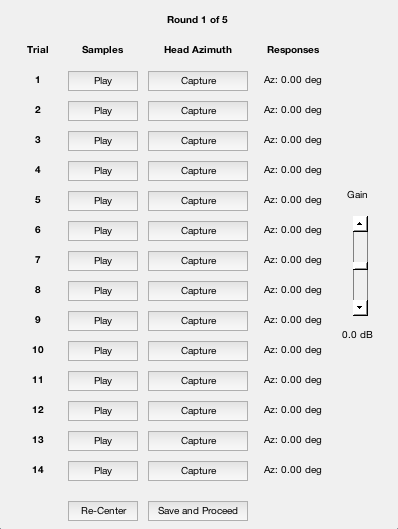
\includegraphics[width=0.58\textwidth]{05_proposed_models/figures/LocalizationTestGUI}}
  \caption{Screenshot of the GUI for the localization test.}
  \label{fig:05_Proposed_Models:Localization_GUI}
\end{figure}

\subsection{Coloration test}\label{sec:05_Proposed_Models:Coloration_Test}
To collect subjective ratings of coloration, we conducted an \citet{ITU-R-BS.1534-3} MUSHRA (MUltiple Stimuli with Hidden Reference and Anchor) test,
administered in the same listening room and with the same headphones, but without head-tracking.%
\footnote{The loudspeaker array which served as a visual reference for the localization test was still present for this test, but the subjects were informed that it no longer corresponded to the signals they would be hearing.}
The test consisted of 1 training round followed by 3 rounds of testing, with optional short breaks between rounds.
In each round, the subject was presented with 9 ``test samples'' (actually 6 test samples, 2 anchors, and a hidden reference) and a labeled reference sample, all of which were a short ($\sim3$~second) clip of pink noise.
The GUI presented to the subject is shown in \figref{fig:05_Proposed_Models:Coloration_GUI} and the sheet of instructions provided to the subject is shown in \figref{fig:05_Proposed_Models:Coloration_Instructions} (at the end of this chapter).
The so-called ``low anchor'' used was the standard $3.5$~kHz low-pass-filtered version of the reference \citep{ITU-R-BS.1534-3}; the second anchor used was a high-shelf-filtered version of the reference, with $+6$~dB of gain applied above $7$~kHz.
The samples were randomly-ordered, but all samples in each round were from a single intended source direction.
The intended source directions produced in the test corresponded to $-45^\circ,~0^\circ,~30^\circ$ azimuth on the horizontal plane, as illustrated by the crosses in \figref{fig:Test_Geometry}.
The subject was asked to judge (and rate on a scale from 0--100) the extent to which each test sample \textit{differs}, in terms of the tonal coloration only, from the labeled reference sample.
As is standard in a MUSHRA test, a rating of 100 indicates that the sample is \textit{indistinguishable} from the reference,
while any rating less than 100 indicates that the sample differs from the reference.
All responses for each round and each subject were linearly mapped (if necessary) such that the low anchor obtained a rating of 0.
In the present dataset, all subjects correctly identified the hidden reference and rated it 100.
The subject was able to repeat each sample (and the labeled reference) any number of times until satisfied with the ratings for that round.

\begin{figure}[t]
  \centering
  \setlength{\fboxsep}{0pt}
  \setlength{\fboxrule}{1pt}
  \fbox{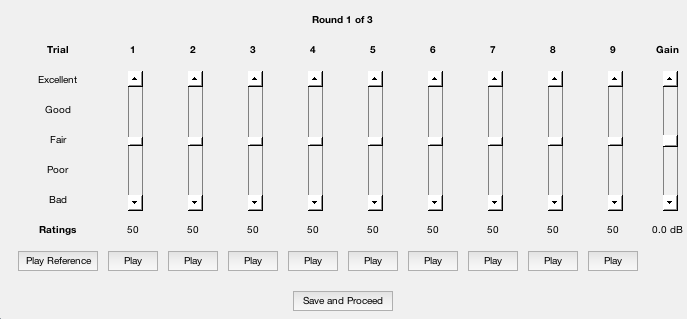
\includegraphics[width=0.99\textwidth]{05_proposed_models/figures/ColorationTestGUI}}
  \caption{Screenshot of the GUI for the coloration test.}
  \label{fig:05_Proposed_Models:Coloration_GUI}
\end{figure}

\section{Results and discussion}\label{sec:05_Proposed_Models:Results}
In the following sections, we present and discuss both the determination of optimal parameters for the localization model and the construction of the coloration models based on the data collected in the listening experiments described above.

%% Localization results
\subsection{Comparison of localization models}\label{sec:05_Proposed_Models:Localization_Results}
Using the measured perceived source directions from the localization experiment (described in \secref{sec:05_Proposed_Models:Localization_Test}), we first determined optimal parameter values (for each of the 4 parameters discussed in \secref{sec:05_Proposed_Models:Localization_Model}) separately for both the velocity and energy vector models.
The optimization consisted of minimizing the squared-residuals between the predicted and measured localization azimuths.
The resulting parameter values are listed in \tabref{tab:Vector_Parameters}.
From these optimal values, we see that, generally, the low-frequency (velocity) vector requires a ``coarser'' set of input data, as the spatial resolution (related to $Q$) is much lower.
Conceptually, this agrees with the notion that low-frequency sounds are not very directional, so a low-spatial-resolution representation of such information should be adequate.
Similarly, the wavelet lengths (set by $\tau_\text{w}$) are longer for the velocity vector than for the energy vector, which is likely a result of low-frequency information requiring longer time-scales in order to be adequately represented.

\begin{table}[t]
\centering
 \begin{tabular}{|c|c|c|c|} \hline
 \textbf{Parameter} & \textbf{Velocity} & \textbf{Energy} & \textbf{Description} \\ \hline
 $Q$ & 9 & 36 & Number of plane-waves \\
 $\alpha$ & 0.95 & 0.7 & Stationary signal weight \\
 $\tau_\text{w}$~(ms) & 2 & 1 & Minimum wavelet half-length \\
 $G_\text{min}$~(dB) & $-8$ & $-30$ & Wavelet detection threshold \\ \hline
 \end{tabular}
 \caption[Optimal parameters for the proposed localization model.]{
 Optimal parameters for each localization vector (velocity and energy).
 More detailed descriptions of each parameter are given in \secref{sec:05_Proposed_Models:Localization_Model}.}
 \label{tab:Vector_Parameters}
\end{table}

In \figref{fig:Localization_Model_Comparison}, the measured localization directions are plotted against the predictions of each model.
The mean absolute prediction error is given by
\begin{equation}
\bar{\epsilon} = \frac{1}{N_\text{r}} \sum_{j = 1}^{N_\text{r}} | \phi_j - \phi_p |,
\end{equation}
where $N_\text{r}$ is the total number of responses, $\phi_j$ is the measured azimuth for response $j$, and $\phi_p$ is the predicted azimuth.
These errors, as well as the squared residuals and Pearson correlation coefficients for the data, are given in \tabref{tab:Localization_Model_Results}.
From these values, we see that the proposed model seems to better predict the data than does the binaural model, as the former achieves a lower squared-residual value, a higher correlation with the data, and a smaller mean absolute prediction error.
This is somewhat surprising given the binaural model's capacity to take into account both subject-dependent variations, since the predictions are made on a per-subject basis (see \secref{sec:04_Auditory_Models:Binaural_Localization_Model}), as well as any effects of the binaural rendering approach used.
The proposed model, on the other hand, is unaware of the binaural rendering approach used and can only make a single prediction per sample, meaning that any subject-dependent variation in the data cannot be captured.
However, unlike the proposed model, the binaural model does not have any free parameters and, accordingly, did not need to be tuned to fit the data.

\begin{table}[t]
\centering
 \begin{tabular}{|c|c|c|c|} \hline
 \textbf{Model Name} & \textbf{Residuals} & \textbf{Correlation} & $\bar{\epsilon}$ \\ \hline
 Proposed & 706.5 & 0.85 & $3.67^\circ$ \\
 \citet{Dietz2011} & 877.0 & 0.81 & $4.36^\circ$ \\ \hline
 \end{tabular}
 \caption[Prediction errors and correlation coefficients for each localization model.]{
 Squared residuals, Pearson correlation coefficients, and mean absolute prediction errors ($\bar{\epsilon}$) for each localization model.
 The squared residuals are normalized by the variance seen in the measured data for each sample.}
 \label{tab:Localization_Model_Results}
\end{table}

\begin{figure}[t]
\centering
  \begin{subfigure}[b]{0.49\columnwidth}
        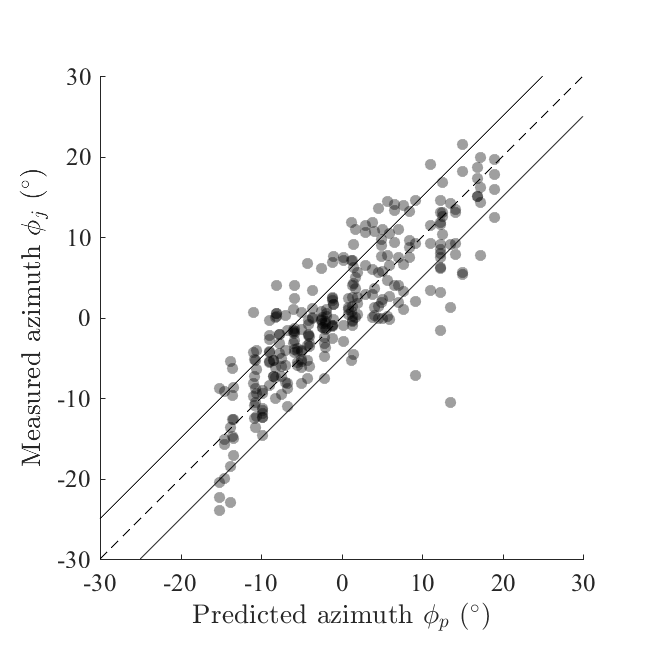
\includegraphics[width=\textwidth]{05_proposed_models/figures/LocalizationModelResults}
        \caption{Proposed model}
        \label{fig:Localization_Model_Results}
  \end{subfigure}
  \hfill
  \begin{subfigure}[b]{0.49\columnwidth}
        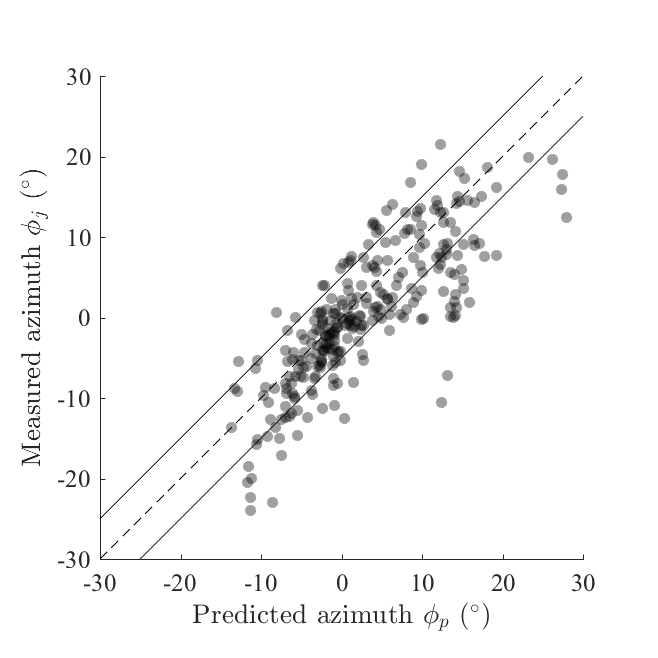
\includegraphics[width=\textwidth]{05_proposed_models/figures/DietzLocalizationResults}
        \caption{\citet{Dietz2011} model}
        \label{fig:Dietz_Localization_Results}
  \end{subfigure}
  \caption[Scatter plots of measured versus predicted source directions.]{
  Scatter plots of measured versus predicted source directions.
  The transparent filled circles indicate the data and model values;
  the dashed lines indicate ideal model results (i.e., $\phi_j = \phi_p$);
  the solid lines indicate discrepancies of $5^\circ$ (i.e., $\phi_j = \phi_p \pm 5^\circ$).}
  \label{fig:Localization_Model_Comparison}
\end{figure}

For both models we observe two outlying data points at approximately $(\phi_p, \phi_j) = (+10^\circ, -10^\circ)$, for which the predicted directions are to the listener's left ($+$), while that subject (both of these data points are from the same subject) localized the sound to the right ($-$).
Although not shown here, the same data points appear again as outliers when plotted against the \textit{intended} source direction, suggesting that these outliers could well be due to an error on the part of the subject.

%% Coloration results
\subsection{Comparison of coloration models}\label{sec:05_Proposed_Models:Coloration_Results}
Using the MUSHRA ratings collected from the coloration listening test (described in \secref{sec:05_Proposed_Models:Coloration_Test}), we performed linear regressions for each model listed in \secref{sec:05_Proposed_Models:Coloration_Models}.
We first converted the MUSHRA ratings to ``coloration scores'', given by $C = 100 - M$, where $M$ are the MUSHRA ratings.
Through this transformation, a reference sample will always have a coloration score of zero, while the low-pass anchor will have a coloration score of 100.
We then computed linear regressions between the values of the metrics in each of the four models and the coloration scores.
Note that, for the binaural models (\citet{Pulkki1999} and \citet{Wittek2007}), we computed each metric on a per-subject basis, i.e., using each subject's individualized HRTFs to render to binaural and subsequently computing per-subject values of each metric.

In building the coloration models, an analysis of the statistical significance of each model parameter revealed that, for the proposed model, neither $\sigma_\eta$ nor $E_{\text{pk}}$ provided a significant improvement to the model.
This is likely because, for all of our test samples, both $\sigma_\eta$ and $E_{\text{pk}}$ were strongly correlated with $\rho_\eta$.
Consequently, our proposed model uses only $\rho_\eta$ and $E_\text{n}$.
Additionally, a ``$y$-intercept'' (offset) term was considered for each model, but was found to be statistically insignificant in all cases.%
\footnote{This is likely because all of the reference samples, by definition, obtain zero coloration scores and zero values for each metric.}
The final formulae and corresponding Pearson correlation coefficients between the measured and predicted coloration scores are tabulated in \tabref{tab:Coloration_Model_Formulas}.
These correlation coefficients suggest that the proposed model is best able to predict the measured coloration scores.

The proposed model is also the only model to have both coefficients positive, even though all of the metrics listed in \secref{sec:04_Auditory_Models:Coloration_Metrics} produce positive values for non-flat spectra.
This indicates that both metrics in the proposed model directly contribute to perceived coloration.
We also note the similarity between the two binaural models (\citet{Pulkki1999} and \citet{Wittek2007}), in both the coefficients and performance of the model.
This may be explained by both models capturing essentially the same information through combining the binaural spectra (see \secreftwo{sec:04_Auditory_Models:Coloration_Metrics:Pulkki_CLL}{sec:04_Auditory_Models:Coloration_Metrics:Wittek_IS}).

\begin{table}[t]
\centering
 \begin{tabular}{|c|c|c|} \hline
 \textbf{Model Name} & \textbf{Formula} & \textbf{Correlation} \\ \hline
 Proposed & $C = 2.88 \rho_\eta + 1.74 E_\text{n}$ & 0.84 \\
 \citet{Kates1984} & $C = -3.20 \rho_{e_\text{CS}} + 54.16 \sigma_{e_\text{CS}}$ & 0.72 \\
 \citet{Pulkki1999} & $C = 9.84 \rho_{e_\text{CLL}} - 18.38 \sigma_{e_\text{CLL}}$ & 0.77 \\
 \citet{Wittek2007} & $C = 10.35 \rho_{e_\text{IS}} - 19.58 \sigma_{e_\text{IS}}$ & 0.77 \\ \hline
 \end{tabular}
 \caption[Formulae and correlation coefficients for each coloration model.]{
 Formulae and Pearson correlation coefficients for each coloration model.
 All correlation $p$-values were less than $10^{-17}$.}
 \label{tab:Coloration_Model_Formulas}
\end{table}

Additionally, in \figref{fig:Coloration_Model_Comparison}, the measured coloration scores are plotted against the predicted scores for each model.
From these plots, we see that the proposed model produces the most compact (towards the $y = x$ line) distribution of the data.
We also note that the model of \citet{Kates1984} is the only model that consistently under-predicts the low anchor scores (as indicated by the cluster of data points at approximately $(75,100)$ in the second plot).
This suggests that this model did not have sufficient degrees of freedom (since the two metrics were strongly correlated with one another) to both capture the end points of the data and fit the intermediate points.

\begin{figure}[t]
\centering
  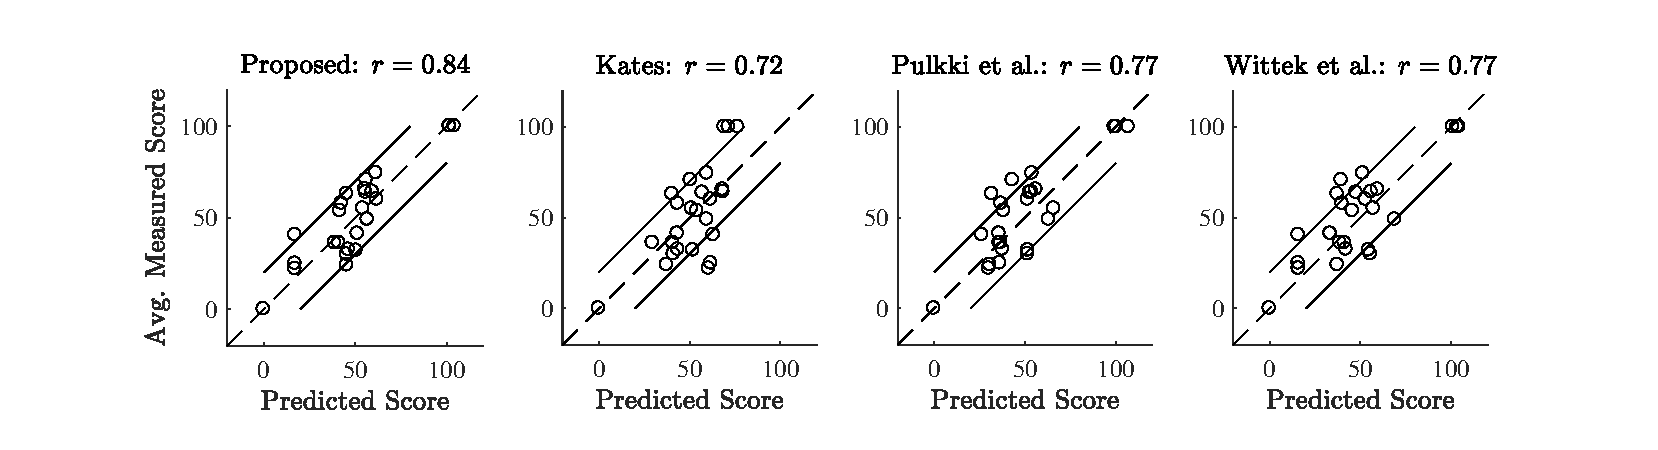
\includegraphics[width=0.99\textwidth,trim={2.15cm 0.3cm 2.3cm 0.5cm},clip]{05_proposed_models/figures/ColorationModelComparison}
  \caption[Scatter plots of average measured versus predicted coloration scores.]{
  Scatter plots of average measured versus predicted coloration scores for each model.
  The empty circles indicate the data and model values;
  the dashed lines indicate ideal model results (i.e., $y = x$);
  the solid lines indicate discrepancies of 20 points (i.e., $y = x \pm 20$).
  The predicted coloration scores for the binaural models (\citet{Pulkki1999} and \citet{Wittek2007}) are averaged across listeners.
  Correlation coefficients for each set of data are given at the top of each plot.}
  \label{fig:Coloration_Model_Comparison}
\end{figure}

\begin{figure}[t]
  \centering
  \setlength{\fboxsep}{0pt}
  \setlength{\fboxrule}{1pt}
  \fbox{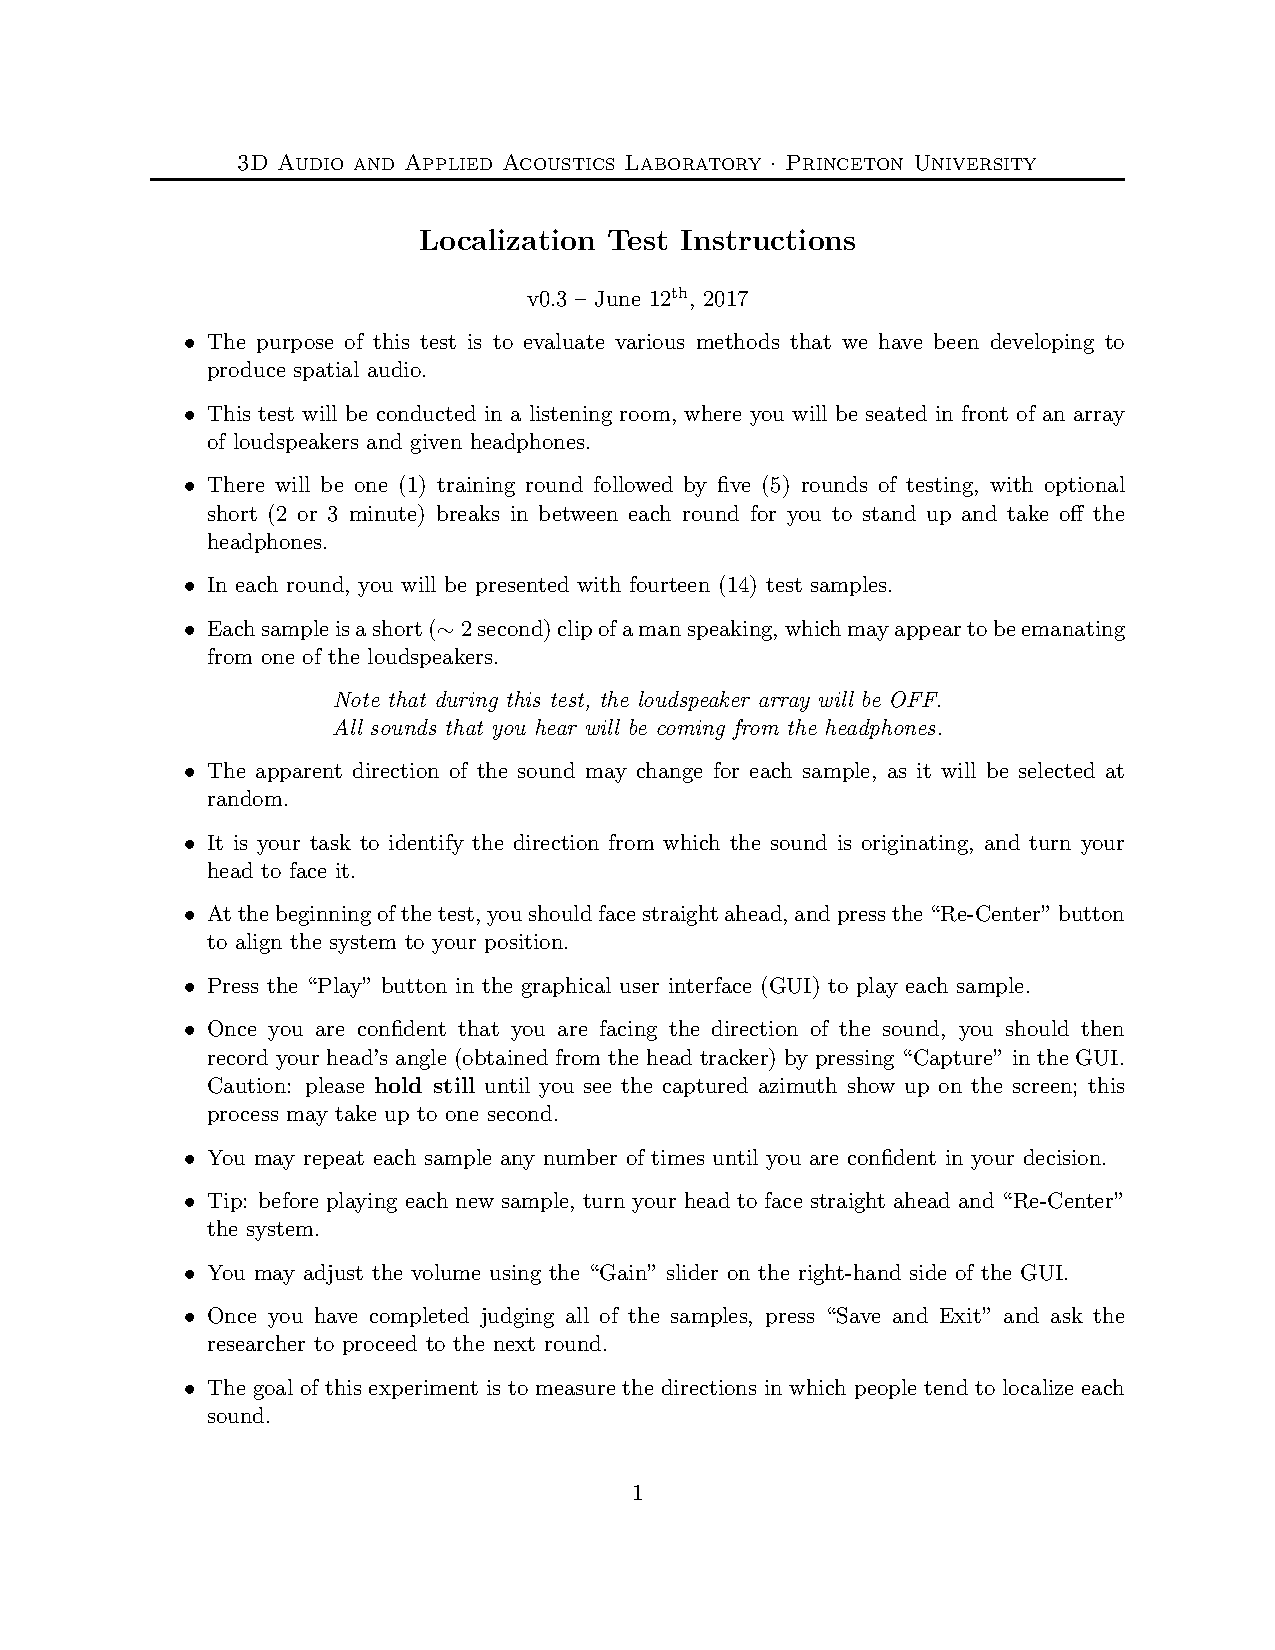
\includegraphics[page=1,width=0.99\textwidth]{05_proposed_models/figures/test_instructions}}
  \caption{Instructions provided to each subject for the localization test.}
  \label{fig:05_Proposed_Models:Localization_Instructions}
\end{figure}

\begin{figure}[t]
  \centering
  \setlength{\fboxsep}{0pt}
  \setlength{\fboxrule}{1pt}
  \fbox{\includegraphics[page=2,width=0.99\textwidth]{05_proposed_models/figures/test_instructions}}
  \caption{Instructions provided to each subject for the coloration test.}
  \label{fig:05_Proposed_Models:Coloration_Instructions}
\end{figure}

\section{Conclusions}\label{sec:05_Proposed_Models:Conclusions}
In this work, we developed models for perceived source localization and spectral coloration.
We empirically determined values for the parameters of these models through comparison with results of subjective listening experiments that we conducted.
The primary advantage of these models, compared to existing binaural ones, is that they do not require rendering ambisonics to binaural.
This allows the models to be used to directly evaluate navigational methods for ambisonics-encoded sound fields, without introducing extraneous factors such as the choice of ambisonics-to-binaural rendering approach or of HRTF.%
\footnote{While it is our expectation that such extraneous factors will necessarily conflate their corresponding errors with those introduced by the navigational method under test, it is worth noting that the relative magnitudes of such errors have not been established.
This remains a topic for further study.}

The localization model (described in \secref{sec:05_Proposed_Models:Localization_Model}) extends a recently-developed precedence-effect-based energy vector model \citep{Stitt2016} in order to predict perceived source localization directly from the ambisonics impulse responses.
To determine parameters of the model, we conducted a virtual localization test (described in \secref{sec:05_Proposed_Models:Localization_Test}) with individualized binaural rendering over head-tracked and equalized headphones.
The predictions of the localization model (see \secref{sec:05_Proposed_Models:Localization_Results}) are in good agreement with the results of this localization test, achieving a mean absolute prediction error of $3.67^\circ$.
Furthermore, the proposed model performs comparably to, if not better than, the binaural localization model of \citet{Dietz2011} (described in \secref{sec:04_Auditory_Models:Binaural_Localization_Model}), in terms of its agreement with the data.

Two important caveats to this result are 1) that the model requires experimental data in order to determine values for its free parameters and 2) that these values are not necessarily valid over any conditions other than those tested.
Indeed, it is worth emphasizing that this model has only been validated for frontal ($\pm20^\circ$ azimuth) sources and a speech signal.
However, given the accuracy of the predictions yielded by the model and the relatively small number of degrees of freedom compared to the number of data points, we conclude that the \textit{structure} of the model is generally valid.
Therefore, we take the parameter values determined here to define a default specification of the model, which we can expect to provide \textit{plausible} predictions of source localization, even though the accuracy of those predictions will almost certainly degrade for any conditions other than those tested here.
The magnitudes of such degradations under other conditions (e.g., source positions, navigational methods, stimuli, etc.) remain to be determined.

Future refinements to this model might pursue reducing its number of free parameters by developing (possibly empirical) models for those parameters based on some input data.
For example, one might seek a model for the stimulus-dependent stationary signal weight ($\alpha$), which is currently determined empirically by fitting model predictions to experimental data (see \citet{Stitt2016,Stitt2017}), such that it can be determined \textit{a priori} for a given stimulus.%
\footnote{\citet{Stitt2016} suggest a simple model for $\alpha$ based on interaural time differences of leading and lagging signals, but no direct relationship between the stimulus and $\alpha$ is given.}

The coloration model uses only the omnidirectional ambisonics impulse responses (i.e., the free-field transfer functions) and predicts a perceived ``coloration score'' from a linear combination of two metrics (defined in \secref{sec:04_Auditory_Models:Coloration_Metrics}): the range of the auditory band spectral error ($\rho_\eta$) and the notch errors ($E_\text{n}$).
To construct this model, we conducted a MUSHRA \citep{ITU-R-BS.1534-3} test (described in \secref{sec:05_Proposed_Models:Coloration_Test}) and performed a linear regression of the metrics with the collected subjective ratings of coloration.
We compared the proposed model to several alternative models and found it to achieve the highest correlation to the measured data (see \secref{sec:05_Proposed_Models:Coloration_Results}).

As with the localization model, the validity of the proposed coloration model has only been established for a limited set of conditions.
Additionally, predicting these ``coloration scores'' is a somewhat artificial task, as the scale (0--100) is arbitrary, and there is no reason to think that the perceived coloration should be strictly linearly related to any of the metrics used.
Nevertheless, a more general result of this analysis is that the metrics used in the proposed model ($\rho_\eta$ and $E_\text{n}$) are dominant factors in the perception of coloration.
Thus, each of these metrics may serve as a useful measure of perceptible spectral coloration, as a large value for either metric would almost certainly entail perceptible coloration.

Ultimately, in order to more rigorously establish their psychoacoustic relevance, the auditory models proposed here should be further validated through additional listening experiments with more subjects and spanning a wider range of conditions.
%The coloration model in particular should be validated for a larger set of navigational methods, since the spectral colorations considered in this work may or may not be comparable to those induced by alternative methods.
Despite this eventual need for further validation, we expect that these models will nonetheless yield valuable insights when evaluating navigational methods.
Consequently, comprehensive comparisons of existing navigational methods should be conducted using these models in order to quantify the penalties incurred by each method, and ultimately determine limits of usability for each method (e.g., maximum translation distance with $\leq 5^\circ$ source localization error).
Indeed, throughout the rest of the present thesis, we employ both the proposed localization model to predict localization and the spectral error metric, $\rho_\eta$, as a measure of perceived coloration.

\section*{Acknowledgements}
The ambisonics room impulse responses were recorded using the Eigenmike by mh Acoustics \citep{EigenmikeURL}.
The present author wishes to thank P.~Stitt for providing the MATLAB code for the precedence-effect-based energy vector model (available online).\citefooturl{StittCodeURL}
This work was approved by the Institutional Review Board for human subjects research at Princeton University,
and was originally presented by \citeauthor{TylkaChoueiri2017a} at the 173\textsuperscript{rd} Meeting of Acoustical Society of America (Acoustics '17 Boston) and published in \textit{Proceedings of Meetings on Acoustics} \citep{TylkaChoueiri2017a}.
%%%% SIMULATION FRAMEWORK %%%%
\chapter{Simulation framework for performance characterization}\label{chap:06_Simulation_Framework}
In this chapter, we lay out a simulation framework for characterizing the performance of different navigational techniques.
In the following sections, we describe the geometry of the simulated sound field, define the parameters of the simulations, and enumerate the metrics which will be computed.
In each of the following chapters, we present results characterizing and comparing different navigational methods obtained by conducting the simulations described here.
Additionally, in \chapref{chap:10_Experimental_Validation}, an experimental validation of the simulations is presented.

\section{Microphone and source geometries}\label{sec:06_Simulation_Framework:Geometry}
In this section we present the ambisonics microphone array geometries used in the subsequent numerical simulations.
In both cases described below, the listener traverses a straight line away from the microphone(s), which will allow us to explore any dependence on source azimuth relative to the direction of travel (see \secref{sec:06_Simulation_Framework:Azimuth_Dependence}).

\subsection{Single-microphone array}\label{sec:06_Simulation_Framework:Point_Geometry}
Consider a single-microphone array geometry, illustrated in \figref{fig:06_Simulation_Framework:Point_Geometry}, in which a single ambisonics microphone ($P = 1$) is separated from the origin by a distance $u$ and placed along the longitudinal $x$-axis, such that its position is given by $\vec{u}_1 = (u,0,0)$.
(Recall that, according to our coordinate system described in \secref{sec:02_Acoustical_Theory:Coordinate_System}, the $+x$-axis points forward from the listener, the $+y$-axis points to the left, and the azimuth $\phi$ measures the angle away from straight ahead.)
In this configuration, we define the \textit{navigable region} as the segment of the $x$-axis connecting the origin and microphone position, i.e., all listener positions $\vec{r}_0 = (x_0, 0, 0)$ where $x_0 \in [0,u]$.

% Diagram of source/mic positions
\begin{figure}[t]
\centering
  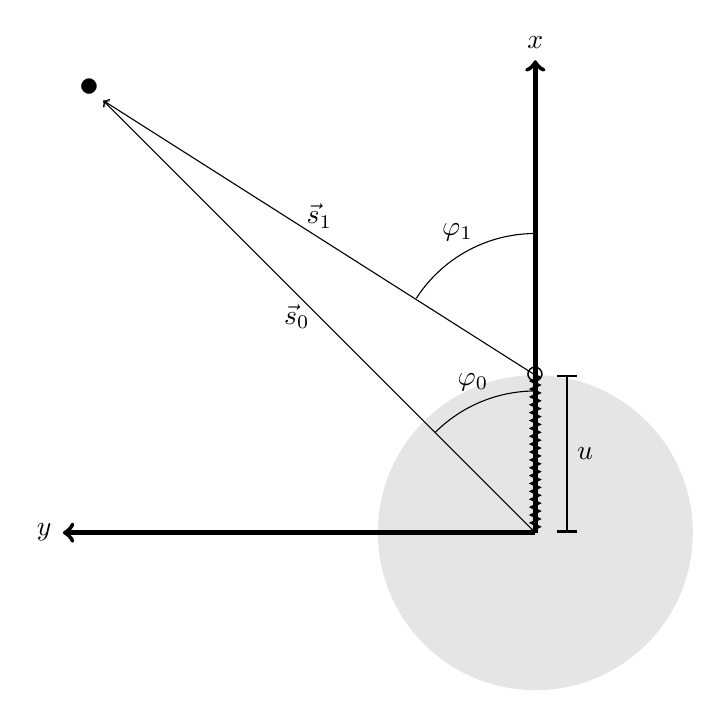
\begin{tikzpicture}[scale=4]
% Parameters
\def\radius{1.5};
\def\arrowScale{0.97};

\def\micSpacing{1};
\def\micL{-0.5*\micSpacing};

\def\sourceRadius{2};
\def\sourceAzimuth{45}
\pgfmathsetmacro\sourceY{cos(-\sourceAzimuth)*\sourceRadius}
\pgfmathsetmacro\sourceX{sin(-\sourceAzimuth)*\sourceRadius}

\pgfmathsetmacro\sourceLAzimuth{-atan(\sourceX/(\sourceY+\micL))}

\def\arcRadius{0.45};
\pgfmathsetmacro\arcY{cos(-\sourceAzimuth/2)*\arcRadius}
\pgfmathsetmacro\arcX{sin(-\sourceAzimuth/2)*\arcRadius}
\pgfmathsetmacro\arcLY{cos(-\sourceLAzimuth/2)*\arcRadius}
\pgfmathsetmacro\arcLX{sin(-\sourceLAzimuth/2)*\arcRadius}

% Coordinate system
\draw[ultra thick,->] (0,0) -- (0,\radius) node[above]{$x$};
\draw[ultra thick,->] (0,0) -- (-\radius,0) node[left]{$y$};

% Arrows
\node at (\sourceX,\sourceY){\Large $\bullet$}; % source
\draw[->] (0,0) -- (\arrowScale*\sourceX,\arrowScale*\sourceY) node[left, pos=0.5]{$\vec{s}_0$}; % origin
\draw[->] (0,-\micL) -- (\arrowScale*\sourceX,\arrowScale*\sourceY) node[above, pos=0.5]{$\vec{s}_1$}; % mic
\draw[thick, decoration = {zigzag, segment length = 1mm, amplitude = 0.5mm}, decorate] (0,0) -- (0,-\micL); % navigable region

% Arcs
\draw[domain=90:(90+\sourceAzimuth)] plot ({\arcRadius*cos(\x)}, {\arcRadius*sin(\x)});
\node at (1.15*\arcX,1.15*\arcY){$\varphi_0$};

%\draw[dashed,->] (\micL,0) -- (\micL,\arcRadius); % left mic
\draw[domain=90:(90+\sourceLAzimuth)] plot ({\arcRadius*cos(\x)}, {\arcRadius*sin(\x) - \micL});
\node at (1.15*\arcLX,1.15*\arcLY - \micL){$\varphi_1$};

% Mic positions
\node at (0,-\micL){\Large $\circ$};
\draw[thick,|-|] (0.1,0) -- (0.1,-\micL) node[right, pos=0.5]{$u$};

\fill [color=black,opacity=0.1] (0,0) circle (\micSpacing/2);

\end{tikzpicture}
  \caption[Diagram of the array geometry for extrapolation simulations.]{
  Diagram of a microphone (empty circle) and a single source (filled circle).
  The shaded gray disk indicates the interior region, where $r < u$.
  The jagged line segment indicates the navigable region, where $x \in [0,u]$ and $y = z = 0$.}
  \label{fig:06_Simulation_Framework:Point_Geometry}
\end{figure}

A single point source is placed on the horizontal plane at $\vec{s}_0 = (s_0 \cos \varphi_0, s_0 \sin \varphi_0, 0)$.
From the position of the microphone, the apparent source position is given by
$\vec{s}_1 = \vec{s}_0 - \vec{u} = (s_1 \cos \varphi_1, s_1 \sin \varphi_1, 0)$,
such that the apparent source azimuth is $\varphi_1$ and the relative source distance from the microphone is $s_1$.

We further define a nondimensional geometrical parameter $\gamma = r / u$.
Here we refer to the region with $\gamma > 1$ as the \textit{exterior region} and that with $\gamma < 1$ as the \textit{interior region} (see \figref{fig:06_Simulation_Framework:Point_Geometry}).

\subsection{Linear microphone array}\label{sec:06_Simulation_Framework:Linear_Geometry}
Consider a linear microphone array geometry, illustrated in \figref{fig:06_Simulation_Framework:Linear_Geometry}, in which a pair of ambisonics microphones ($P = 2$) are separated by a distance $\Delta = 2u$, equidistant from the origin and placed along the lateral $y$-axis, such that their positions are given by $\vec{u}_1 = (0,\Delta/2,0)$ and $\vec{u}_2 = (0,-\Delta/2,0)$.
In this configuration, we define the \textit{navigable region} as the segment of the $y$-axis connecting the two microphone positions, i.e., all listener positions $\vec{r}_0 = (0, y_0, 0)$ where $y_0 \in [-\Delta/2,\Delta/2]$.
Here also we define the same nondimensional geometrical parameter, now given by $\gamma = r / (\Delta / 2) = r / u$.

% Diagram of source/mic positions
\begin{figure}[t]
\centering
  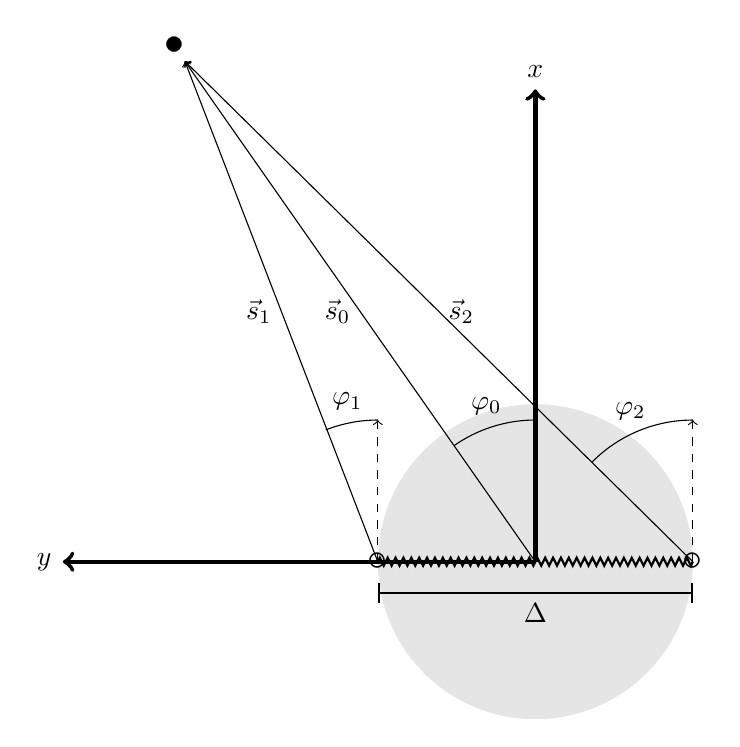
\begin{tikzpicture}[scale=4]
% Parameters
\def\radius{1.5};
\def\arrowScale{0.97};

\def\micSpacing{1};
\def\micL{-0.5*\micSpacing};
\def\micR{0.5*\micSpacing};

\def\sourceRadius{2};
\def\sourceAzimuth{35}
\pgfmathsetmacro\sourceY{cos(-\sourceAzimuth)*\sourceRadius}
\pgfmathsetmacro\sourceX{sin(-\sourceAzimuth)*\sourceRadius}

\pgfmathsetmacro\sourceLAzimuth{-atan((\sourceX-\micL)/\sourceY)}
\pgfmathsetmacro\sourceRAzimuth{-atan((\sourceX-\micR)/\sourceY)}

\def\arcRadius{0.45};
\pgfmathsetmacro\arcY{cos(-\sourceAzimuth/2)*\arcRadius}
\pgfmathsetmacro\arcX{sin(-\sourceAzimuth/2)*\arcRadius}
\pgfmathsetmacro\arcLY{cos(-\sourceLAzimuth/2)*\arcRadius}
\pgfmathsetmacro\arcLX{sin(-\sourceLAzimuth/2)*\arcRadius}
\pgfmathsetmacro\arcRY{cos(-\sourceRAzimuth/2)*\arcRadius}
\pgfmathsetmacro\arcRX{sin(-\sourceRAzimuth/2)*\arcRadius}

% Coordinate system
\draw[ultra thick,->] (0,0) -- (0,\radius) node[above]{$x$};
\draw[ultra thick,->] (0,0) -- (-\radius,0) node[left]{$y$};

% Arrows
\node at (\sourceX,\sourceY){\Large $\bullet$}; % source
\draw[->] (0,0) -- (\arrowScale*\sourceX,\arrowScale*\sourceY) node[left, pos=0.5]{$\vec{s}_0$}; % origin
\draw[->] (\micL,0) -- (\arrowScale*\sourceX,\arrowScale*\sourceY) node[left, pos=0.5]{$\vec{s}_1$}; % left mic
\draw[->] (\micR,0) -- (\arrowScale*\sourceX,\arrowScale*\sourceY) node[right, pos=0.5]{$\vec{s}_2$}; % right mic
\draw[thick, decoration = {zigzag, segment length = 1mm, amplitude = 0.5mm}, decorate] (\micL,0) -- (\micR,0); % navigable region

% Arcs
\draw[domain=90:(90+\sourceAzimuth)] plot ({\arcRadius*cos(\x)}, {\arcRadius*sin(\x)});
\node at (1.15*\arcX,1.15*\arcY){$\varphi_0$};

\draw[dashed,->] (\micL,0) -- (\micL,\arcRadius); % left mic
\draw[domain=90:(90+\sourceLAzimuth)] plot ({\arcRadius*cos(\x) + \micL}, {\arcRadius*sin(\x)});
\node at (1.15*\arcLX + \micL,1.15*\arcLY){$\varphi_1$};

\draw[dashed,->] (\micR,0) -- (\micR,\arcRadius); % right mic
\draw[domain=90:(90+\sourceRAzimuth)] plot ({\arcRadius*cos(\x) + \micR}, {\arcRadius*sin(\x)});
\node at (1.15*\arcRX + \micR,1.15*\arcRY){$\varphi_2$};

% Mic positions
\node at (\micL,0){\Large $\circ$};
\node at (\micR,0){\Large $\circ$};
\draw[thick,|-|] (\micL,-0.1) -- (\micR,-0.1) node[below, pos=0.5]{$\Delta$};

\fill [color=black,opacity=0.1] (0,0) circle (\micSpacing/2);

\end{tikzpicture}
  \caption[Diagram of the array geometry for interpolation simulations.]{
  Diagram of a two-microphone array (empty circles) with a single source (filled circle).
  The shaded gray disk indicates the interior region, where $r < \Delta / 2$.
  The jagged line segment indicates the navigable region, where $y \in [-\Delta/2,\Delta/2]$ and $x = z = 0$.}
  \label{fig:06_Simulation_Framework:Linear_Geometry}
\end{figure}

Similar to the single-microphone case, the apparent source position from the position of the $p^\textrm{th}$ microphone is given by
$\vec{s}_p = \vec{s}_0 - \vec{u}_p = (s_p \cos \varphi_p, s_p \sin \varphi_p, 0)$,
such that the apparent source azimuth is $\varphi_p$ and the relative source distance from that microphone is $s_p$.

\section{Simulation parameters}\label{sec:06_Simulation_Framework:Parameters}
For extrapolation methods, we simulate recording of the sound field depicted in \figref{fig:06_Simulation_Framework:Point_Geometry} for a range of microphone positions, $u \in [0.1, 10]$~m, and all source positions $s_0 = \gamma u$ for $\gamma \in [0.1, 10]$.
In each simulation, we vary the source azimuth from $\varphi_0 = 0^\circ$ to $180^\circ$ in increments of $5^\circ$ and generate an artificial ambisonics impulse response at the microphone.
We then estimate, using each extrapolation method, the ambisonics impulse responses at translated listener positions from $x_0 = 0$ to $u$, taken in 20 equal increments.

For interpolation methods, we simulate recording of the sound field depicted in \figref{fig:06_Simulation_Framework:Linear_Geometry} for a range of microphone spacings, $\Delta \in [0.1, 10]$~m, and all source positions $s_0 = \gamma \Delta / 2$ for $\gamma \in [0.1, 10]$.
For those methods that require interpolation weights, we choose linear interpolation weights for each intermediate position between the microphones.
In each simulation, we vary the source azimuth from $\varphi_0 = 0^\circ$ to $90^\circ$ in increments of $5^\circ$ and generate an artificial ambisonics impulse response at each microphone.
We then estimate, using each interpolation method, the ambisonics impulse responses at intermediate listener positions from $y_0 = -\Delta/2$ to $\Delta/2$, taken in 20 equal increments.

In all simulations, unless stated otherwise, we choose $L_\textrm{in} = 4$ and $L_\textrm{out} = 1$.%
\footnote{Note that, for the metrics listed in \secref{sec:06_Simulation_Framework:Metrics}, only the localization model (described in \secref{sec:05_Proposed_Models:Localization_Model}) depends on $L_\textrm{out}$; all of the other metrics, by construction, use only the zeroth and first order signals.}
The sampling rate is 48~kHz and all impulse responses are calculated with 16,384~samples ($\approx 341$~ms).
Additionally, unless stated otherwise, we filter all point-source ambisonics impulse responses with the near-field compensation high-pass filters given in \eqnref{eq:02_Acoustical_Theory:NearField_HPF}, with order-dependent corner frequencies equal to $f_l = (200 \times l)$~Hz.

\subsection{Source azimuth dependence}\label{sec:06_Simulation_Framework:Azimuth_Dependence}
In order to explore the basic properties of a given navigational method, we consider a representative far-field scenario and compute the effective frequency response induced by translation.
For these simulations, we pick $s_0 = 2.5$~m and $\gamma = 10$ (so $u = 0.25$~m for extrapolation methods and $\Delta = 0.5$~m for interpolation methods) and translate to $\vec{r}_0 = (0, 0, 0)$.
Then, for each source azimuth, we compute the induced frequency response, which is given by the ratio of the zeroth-order translated ambisonics signal, $A_0(k)$, to the zeroth-order reference ambisonics signal, $B_0(k)$, that would have been measured at $\vec{r}_0$.

\section{Metrics}\label{sec:06_Simulation_Framework:Metrics}
We ultimately compute errors incurred through navigation by each method using the following metrics:
\begin{enumerate}
\item the level error, $e_\lambda$, of the mean audible energy (MAE), as given in \secref{sec:04_Auditory_Models:Audible_Energy},
\item the spectral range, $\rho_\eta$, of the auditory band spectral error (ABSE), as given in \secref{sec:04_Auditory_Models:Coloration_Metrics:ABSE},
\item the localization error, $e_\nu$, as given in \eqnref{eq:04_Auditory_Models:Localization_Error}, for the localization vector model proposed in \secref{sec:05_Proposed_Models:Localization_Model}, and
\item the error, $e_\Psi$, in the diffuseness parameter, as given in \secref{sec:04_Auditory_Models:Diffuseness_Parameter}.
\end{enumerate}
In the following chapters, we plot these predicted errors, averaged over the entire navigable region (as defined above) and all source azimuths,%
\footnote{Note that doing so yields an effective navigable region which is disk-shaped relative to a single fixed source position and, due to symmetry, we need only compute these errors on half of the disk.}
for various combinations of source distance $s_0$ and either microphone distance $u$ (for extrapolation methods) or microphone spacing $\Delta$ (interpolation methods).
%%%% CHARACTERIZATION OF EXTRAPOLATION TECHNIQUES %%%%
\chapter{Performance errors incurred by linear extrapolation methods}\label{chap:07_Characterization_Extrapolation}
In this chapter, we evaluate, through a comprehensive set of the numerical simulations described in \chapref{chap:06_Simulation_Framework}, the performance of two extrapolation-based navigational methods.
The methods considered here are chosen for their broad applicability to arbitrary sound fields due to the linear nature of the processing involved.
However, these methods are also susceptible to violating the region of validity restriction (see \secref{sec:02_Acoustical_Theory:Helmholtz_Equation}) if the listener attempts to navigate beyond the distance of the nearest source to the microphone.
Through the analyses presented here, we aim to determine, in terms of the metrics enumerated in \secref{sec:06_Simulation_Framework:Metrics}, the nature and degree of any penalties incurred by violating this region of validity restriction.

%% saved for a paper abstract
%In the first method, a plane-wave decomposition is employed to simplify the translation operation, however different methods and grid distributions for the plane-wave decomposition can introduce varying errors.
%Consequently, these parameters are first explored in isolation via numerical simulations of a single-microphone array, as described in \chapref{chap:06_Simulation_Framework}.
%Results show that matching the number of plane-waves to the number of ambisonics signals and employing the ``beamforming'' plane-wave decomposition method yields the most reliable results.
%%NOTE%% for the paper, make sure we establish right away the universality of this paper in that it should apply to all linear methods

%The second navigational method employs spherical harmonic translation coefficients to directly extrapolate the ambisonics signals.
%Performance errors are characterized for both methods via numerical simulations in terms of the metrics identified in \secref{sec:06_Simulation_Framework:Metrics}.
%Results show that both methods tend to exhibit two distinct regimes of behavior for far- and near-field sources, and that the performance for near-field sources is often degraded (compared to that for far-field sources) due to the violation of the region of validity restriction.
%In particular, both methods were found to incur significant errors in both overall level and localization when the region of validity restriction is violated.
%Additionally, the plane-wave translation method is shown to perform well for far-field sources, whereas the ambisonics translation method yields significant errors which tend to increase steadily with navigation distance.

\section{Introduction}\label{sec:07_Characterization_Extrapolation:Introduction}
According to ambisonics theory (reviewed in \secref{sec:02_Acoustical_Theory:Helmholtz_Equation}), an ambisonics recording of a sound field contains information about the spatial and temporal distribution of sound over the entire spherical free-field region surrounding the microphone (i.e., the so-called \textit{region of validity}) \citep{Williams1999,GumerovDuraiswami2005,Zotter2009PhD}.
However, recall that a finite-order expansion of a sound field yields only an approximation to that sound field, the accuracy of which decreases with increasing frequency and distance from the expansion center \citep{Poletti2005,WardAbhayapala2001} (see \eqnref{eq:01_Introduction:kr_Inequality}), so the prospect of navigating such a sound field is inherently limited.
Fortunately, this limitation is primarily a technical one, since synthetic sound fields can be generated to arbitrarily high orders and microphone array technology%
\footnote{See, for example: the Zylia ZM-1 \citep{ZyliaZM1URL}, the mh acoustics Eigenmike \citep{EigenmikeURL}, and the VisiSonics Audio Camera \citep{VisiSonicsAudioCameraURL}.}
is rapidly advancing such that it may soon be practical to capture very high-order expansions of real sound fields.

The more fundamental limitation of the spherical-harmonic description of sound fields is that the region over which the expansion is valid is limited by the nearest sound source (or scattering body) to the expansion center (as discussed in \secref{sec:02_Acoustical_Theory:Helmholtz_Equation}).
Consequently, near-field sources pose a particularly limiting problem to navigation.
The precise consequences of violating this region of validity restriction have not been clearly determined, and are a primary focus of this chapter.

Several previous studies have developed extrapolation-based navigational methods from a single ambisonics microphone.
In the following section, we provide a critical review of these existing methods and identify the main challenges they face.
All of the methods discussed below are listed in \tabref{tab:01_Introduction:Methods}.

%% PREVIOUS WORK %%
\subsection{Previous work}\label{sec:07_Characterization_Extrapolation:Previous_Work}
Perhaps the most intuitive navigational method is the \textit{virtual ambisonics} method, as described in \secref{sec:03_Navigation_Techniques:VA_Technique}.
In this method, the ambisonics signals are first decoded for a given loudspeaker array, which is then simulated in a virtual space with the listener at any desired position within the array.
The combined signals arriving at the virtual listener from the virtual loudspeaker array are then computed numerically and played back to the real listener.
Some advantages of this method are that we are free of the practical limitations (such as space, floors/walls, cost, etc.) common to physical loudspeaker arrays and that we can leverage the wealth of experience with real ambisonics systems that has been accumulated by researchers in this field.

For example, \citet{Frank2008} showed that so-called ``max-$r_{\textrm{E}}$'' decoding schemes yield more accurate localization at off-center positions and \citet{Satongar2013b} showed that off-center localization improves with increasing ambisonics expansion order.
Also, to account for the finite distances of loudspeakers from the listening position, \citet{Daniel2003b} developed a near-field-compensated decoding scheme which treats the loudspeakers as point-sources and consequently reconstructs the sound field more accurately at off-center locations.

As it has been defined, this method has no knowledge of any source (or obstacle) positions; consequently, depending on the positions of any sources in the sound field, the listener may inadvertently navigate too far such that the region of validity restriction is violated.
This method also inherently introduces a limit on the navigable region of the listener due to the finite size of the virtual array.
Although it remains unclear in what way the performance may degrade if the listener navigates outside the virtual array, the issue would be avoided entirely if plane-wave sources were used, as done in the plane-wave translation method (described in \secref{sec:03_Navigation_Techniques:PW_Technique}).

The \textit{plane-wave translation} method entails computing a plane-wave expansion of the sound field and translating along each plane-wave term.
\citet{MenziesAlAkaidi2007b} first derived the mathematical operations required for this method, although they did so while developing a technique to more accurately render synthetic near-field sources binaurally by way of a plane-wave expansion and translation.
\citet{SchultzSpors2013} later formulated the plane-wave translation method for the purpose of sound field navigation and examined the time- and frequency-domain consequences of the translation operation.
Similar to the virtual ambisonics method described above, this method is also prone to violating the region of validity restriction in the presence of near-field sources.

\citet{HahnSpors2015b} evaluated spectral coloration induced by the method by visually examining impulse and frequency responses and found that the induced coloration is often mitigated by matching $Q$, the number of plane-wave terms, to $N$, the number of ambisonics signals (i.e., the so-called ``critically-sampled'' condition, when $Q = N$) \citep[section 5]{HahnSpors2015b}. % ``friendly aliasing''
In the same study, the authors found that when $Q > N$ (in the so-called ``oversampled'' condition), navigating parallel to the direction of a source introduced less coloration than navigating perpendicularly. % only true in oversampling conditions
The localization properties of this method were explored by \citet{Winter2014}, who showed that the range over which accurate localization is achieved increases with ambisonics expansion order and that increasing the number of plane-wave-expansion terms beyond critically-sampled does not improve localization.
More recently, \citet{TylkaChoueiri2015} evaluated the localization errors using the velocity and energy localization vectors developed by \citet{Gerzon1992}, although the perceptual relevance of the findings of this study are limited since the analysis does not take into account the precedence effect.

Another navigational method, referred to here as \textit{ambisonics translation} and described in \secref{sec:03_Navigation_Techniques:SR_Technique}, is to translate the ambisonics expansion center by re-expanding the sound field about the desired point.%
\footnote{Relatedly, \citet{AhrensSpors2009} proposed a method which uses very similar mathematical operations (Bessel function translations) in order to analytically move in two dimensions the ``sweet-spot'' within a circular loudspeaker array.}
\citet{GumerovDuraiswami2005} derived recurrence relations which enable fast computation of such re-expansions and \citet{Zotter2009PhD} extended those derivations to real-valued spherical harmonics.
A subset of these derivations are replicated in \apxref{chap:A1_Navigation_Filters}.
\citet{MenziesAlAkaidi2007a} in particular described how this method can be used to allow a listener to virtually navigate ambisonics-encoded sound fields, although a detailed analysis was not performed.
More recently, \citet{BaumgartnerZotter2012} discussed time-domain implementation issues of the re-expansion filters and proposed a discrete-time realization with improved stability.
Again, this method is prone to violating the region of validity restriction if a listener navigates beyond the the nearest source to the microphone.

In order to overcome the region of validity restriction, \citet{Wakayama2017} proposed an extrapolation method that is based on spherical-harmonic translation filters but which requires \textit{a priori} knowledge of the source position.
The authors showed that not only does the method enable navigation beyond a near-field source, but also the method is able to estimate the directivity of the source using a multipole expansion.
It is not clear, however, whether or how this method can be extended to accommodate multiple sources.

More recently, \citet{Plinge2018} developed a parametric method which relies on a time-frequency (i.e., short-time Fourier transform) analysis of the sound field from a single first-order ambisonics microphone as well as a previously measured ``distance map'' of the environment.
This distance map is essentially a source-distance lookup table, consisting of the measured (e.g., optically) distance to the nearest obstacle in each direction (azimuth and elevation) from the microphone.
The recorded sound field is first decomposed via directional audio coding (DirAC) \citep{Pulkki2007} in the time-frequency domain into diffuse and directional sound components.
Each directional component is then treated as a virtual point-source, with the direction of the source determined via an acoustic intensity vector calculation (cf.~\citet[Eq.~(11)]{MerimaaPulkki2005} and \secref{sec:04_Auditory_Models:Intensity_Vector} in this thesis) and its distance determined via the distance map for that direction.
The signals from these virtual sources are then ``re-recorded'' by a virtual microphone at an arbitrary position and with arbitrary directivity.%
\footnote{This method is essentially a one-microphone special case of the method proposed by \citet{Thiergart2013}, where the distance map obviates the need for a second microphone for source triangulation.}
By construction, this method is free of the region of validity restriction, as the listener is navigating within a well-defined model of the sound field.
However, it is unclear if this method can accurately capture and reproduce the directivities of the real sources, as the method exclusively uses omnidirectional point sources to model the sound field.

%In a recent study, \citet{FernandezGrande2016} proposed an equivalent source method for representing and reconstructing a measured sound field.
%In this method, the sound field is captured with one (or more) ambisonics microphone(s) and subsequently fitted, in a least-squares sense, to that created by a predefined grid of virtual monopole sources.
%This yields a virtual sound field consisting of a finite set of known monopole sources, which can then be rendered at an arbitrary position elsewhere in the space.
%However, without \textit{a priori} knowledge of the real sound source positions, the performance of the method may degrade.

%% OBJECTIVES AND APPROACH %%
\subsection{Objectives and approach}
In light of the above discussion we identify the following main issues that existing extrapolation-based navigational methods can face:
\begin{enumerate}
%\item the user is restricted to a finite navigable region,
\item the region of validity restriction is violated,
\item localization information is degraded,
\item spectral coloration or other audible processing artifacts are introduced,
\item geometric information about the sound field (e.g., source locations) must be known or inferred,
%\item arbitrary signals cannot be accommodated,
\item arbitrary (e.g., dense or reverberant) sound fields cannot be reproduced, and/or
\item source directivity cannot be captured or reproduced.
\end{enumerate}
In this chapter, we consider only the plane-wave and ambisonics translation methods as they are the only methods (with the exception of the virtual ambisonics method, which is not significantly different from the plane-wave translation method) that are broadly applicable to arbitrary sound fields with an arbitrary placement of sources (i.e., these methods do not suffer from issues 4 or 5).
However, since these methods are not directly aware of source positions, they are prone to violating the region of validity restriction (issue 1).
We aim to investigate the penalties (in terms of localization errors and spectral colorations, issues 2 and 3, as well as other perceptually-relevant performance metrics) incurred when this restriction is violated.
Both methods may also preserve source directivity information (issue 6), but we do not explore this here.

The objectives of the present work are to determine the penalties incurred by violating the region of validity restriction and to characterize and compare the performance of the plane-wave and ambisonics translation methods.

To these ends, we perform numerical simulations, as described in \chapref{chap:06_Simulation_Framework}, of both methods and use objective metrics to evaluate the errors introduced by each method in terms of sound level, spectral coloration, source localization, and diffuseness.
First, in \secref{sec:07_Characterization_Extrapolation:Plane-wave_Dependence}, we conduct simulations of a typical far-field scenario in order to objectively determine (in terms of these metrics) suitable parameters for the plane-wave decomposition calculation required for the plane-wave translation method.
Next, in \secref{sec:07_Characterization_Extrapolation:Azimuth_Dependence}, we explore basic properties of each method by computing the effective frequency responses induced by translation for various source azimuths.
We then present and discuss in \secref{sec:07_Characterization_Extrapolation:Results} the results of simulations characterizing and comparing the performance of both methods.
Finally, conclusions indicated by these results are summarized in \secref{sec:07_Characterization_Extrapolation:Conclusions}.

\section{Plane-wave decomposition parameters}\label{sec:07_Characterization_Extrapolation:Plane-wave_Dependence}
In this section, we compare two methods for performing plane-wave decomposition:
\begin{enumerate}
\item beamforming, as given by \eqnref{eq:02_Acoustical_Theory:A2mu}, and
\item pseudoinversion, as given by \eqnref{eq:02_Acoustical_Theory:A2mu_Pinv}.
\end{enumerate}
In particular, we explore the performance of each method across a range plane-wave grid densities and input ambisonics orders, $L_\text{in}$.
For all plane-wave expansions, we compute $Q$ plane-wave terms arranged on Fliege nodes and use the corresponding quadrature weights (available online).\citefooturl{FliegeNodesURL}
Additionally, for ease of comparison with $L_\text{in}$, we define the ``order'' of a given plane-wave expansion as $\sqrt{Q} - 1$.
As mentioned in \secref{sec:06_Simulation_Framework:Metrics}, all errors are computed averaging over all source azimuths and over all listener positions in the navigable region (see \figref{fig:06_Simulation_Framework:Point_Geometry}).
For these simulations, we examine a typical far-field scenario by choosing $u = 0.25$~m and $s_0 = 2.5$~m (so $\gamma = 10$).

%\subsection{Results}
In \figreftwo{fig:07_Characterization_Extrapolation:Level_Order:PWT-bf}{fig:07_Characterization_Extrapolation:Level_Order:PWT-pinv}, we plot the level errors (as defined in \secref{sec:04_Auditory_Models:Audible_Energy}) for each plane-wave decomposition method as a function of $Q$ and $L_\text{in}$.
From \figref{fig:07_Characterization_Extrapolation:Level_Order:PWT-bf}, we note a region of small errors that follows the diagonal line $L_\text{in} \approx \sqrt{Q} - 1$.
This suggests that, for the beamforming method, it is advantageous to match the number of plane-wave terms to the number of ambisonics signals, i.e., $Q \approx N_\text{in}$.
Following \citet{HahnSpors2015b}, we refer to this condition as the ``critically-sampled'' condition, since $Q = N_\text{in}$, while we refer to $Q > N_\text{in}$ as oversampled and $Q < N_\text{in}$ as undersampled.

\begin{figure*}[t]
    	\centering
    	\begin{subfigure}[b]{0.49\textwidth}
        		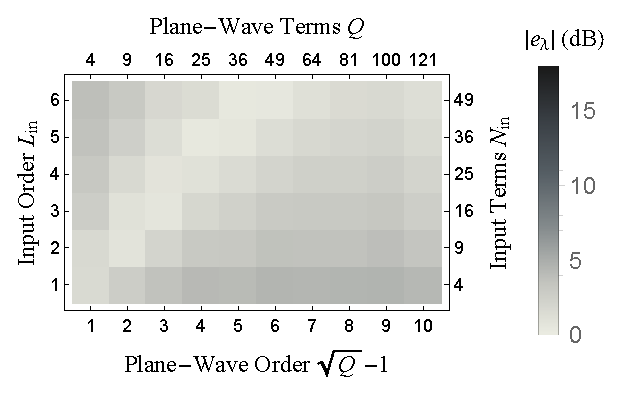
\includegraphics[width=\textwidth]{07_characterization_extrapolation/figures/audibleEnergy_order_pwt-bf.eps}
        		\caption{Level error $e_\lambda$ -- beamforming}
        		\label{fig:07_Characterization_Extrapolation:Level_Order:PWT-bf}
    	\end{subfigure}
	\hfill
    	\begin{subfigure}[b]{0.49\textwidth}
        		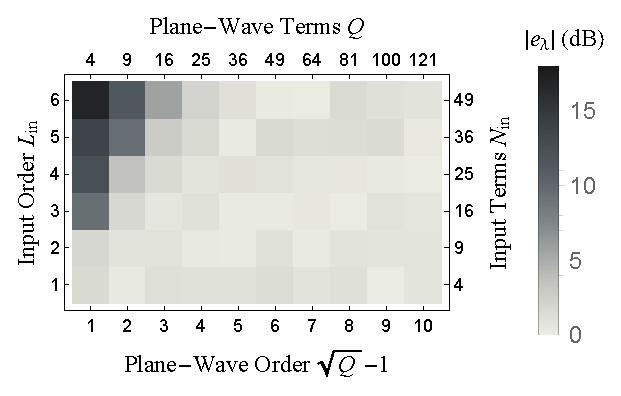
\includegraphics[width=\textwidth]{07_characterization_extrapolation/figures/audibleEnergy_order_pwt-pinv.eps}
        		\caption{Level error $e_\lambda$  -- pseudoinversion}
        		\label{fig:07_Characterization_Extrapolation:Level_Order:PWT-pinv}
    	\end{subfigure}
	
	\vspace{0.5cm}
	\begin{subfigure}[b]{0.49\textwidth}
        		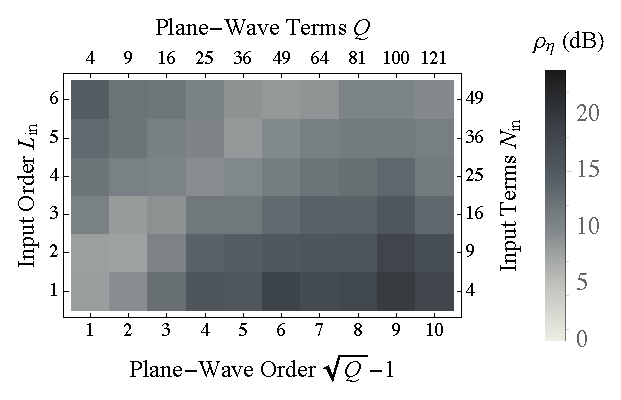
\includegraphics[width=\textwidth]{07_characterization_extrapolation/figures/scharer2009_order_pwt-bf.eps}
        		\caption{Spectral error $\rho_\eta$ -- beamforming}
        		\label{fig:07_Characterization_Extrapolation:Spectral_Order:PWT-bf}
    	\end{subfigure}
	\hfill
    	\begin{subfigure}[b]{0.49\textwidth}
        		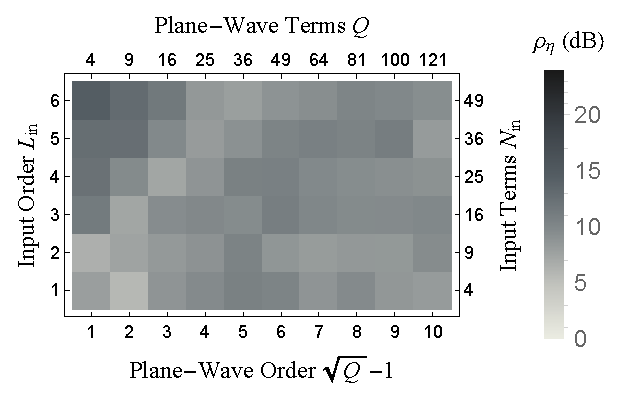
\includegraphics[width=\textwidth]{07_characterization_extrapolation/figures/scharer2009_order_pwt-pinv.eps}
        		\caption{Spectral error $\rho_\eta$ -- pseudoinversion}
        		\label{fig:07_Characterization_Extrapolation:Spectral_Order:PWT-pinv}
    	\end{subfigure}
	
	\caption[Dependence of errors on plane-wave terms and ambisonics input order.]{
	Dependence of errors on $Q$ and ambisonics input order $L_\text{in}$ (continued on p.~\pageref{fig:07_Characterization_Extrapolation:PWT_Order_Dependence:contd}).}
	\label{fig:07_Characterization_Extrapolation:PWT_Order_Dependence}
\end{figure*}

From \figref{fig:07_Characterization_Extrapolation:Level_Order:PWT-pinv}, we see a similar region of small errors, but it is less pronounced, since for $Q > N_\text{in}$ (bottom right corner of the plot), the errors are also small.
However, we note that a region of very large errors exists where $Q < N_\text{in}$ (top left corner).
This suggests that, for the pseudoinversion method, it is advantageous to have $Q \geq N_\text{in}$;
i.e., to have at least as many plane-wave terms as ambisonics signals.

The spectral errors (as defined in \secref{sec:04_Auditory_Models:Coloration_Metrics:ABSE}) for each method are plotted in \figreftwo{fig:07_Characterization_Extrapolation:Spectral_Order:PWT-bf}{fig:07_Characterization_Extrapolation:Spectral_Order:PWT-pinv}, which show trends similar to those exhibited by the level errors discussed above.
From these plots, it is clear that only the critically-sampled condition is ideal for the beamforming method.
This is in agreement with the finding of \citet[cf.~Fig.~7]{HahnSpors2015b}: that the critical-sampling condition yields decreased coloration (compared to oversampling) when using the beamforming method.
From \figref{fig:07_Characterization_Extrapolation:Spectral_Order:PWT-pinv}, we see that both the critical-sampling and oversampling conditions yield small errors for the pseudoinversion method.
Oversampling and undersampling for the beamforming method, as well as undersampling for the pseudoinversion method, all yield significantly larger errors than other conditions.

From \figreftwo{fig:07_Characterization_Extrapolation:Localization_Order:PWT-bf}{fig:07_Characterization_Extrapolation:Localization_Order:PWT-pinv}, we see that both methods yield large localization errors (as computed with \eqnref{eq:04_Auditory_Models:Localization_Error} for the localization model described in \secref{sec:05_Proposed_Models:Localization_Model}) for undersampled conditions.
For the beamforming method, the errors are otherwise uniformly small, except at very small ambisonics orders ($L_\text{in} = 1$).
That these errors do not improve with increasing $Q$ corroborates the finding of \citet[cf.~Fig.~4]{Winter2014}: that increasing the number of plane-waves beyond critically-sampled does not improve localization when using the beamforming method.
From \figref{fig:07_Characterization_Extrapolation:Localization_Order:PWT-pinv}, we see that the pseudoinversion method appears sensitive to mismatches between $Q$ and $N_\text{in}$ given the presence of large, sporadic errors that do not follow any obvious pattern.

\begin{figure*}[t]\ContinuedFloat
	\begin{subfigure}[b]{0.49\textwidth}
        		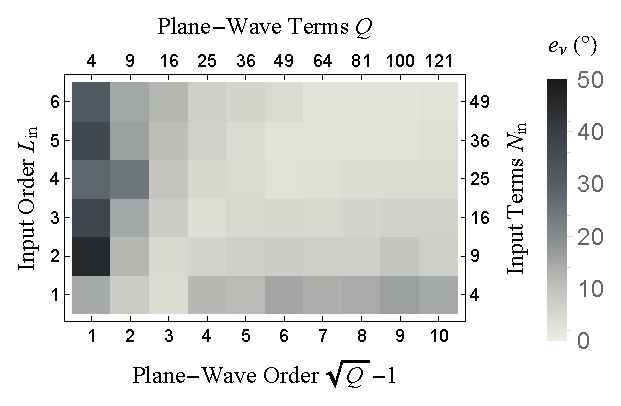
\includegraphics[width=\textwidth]{07_characterization_extrapolation/figures/tylka2017_order_pwt-bf.eps}
        		\caption{Localization error $e_\nu$ -- beamforming}
        		\label{fig:07_Characterization_Extrapolation:Localization_Order:PWT-bf}
    	\end{subfigure}
	\hfill
    	\begin{subfigure}[b]{0.49\textwidth}
        		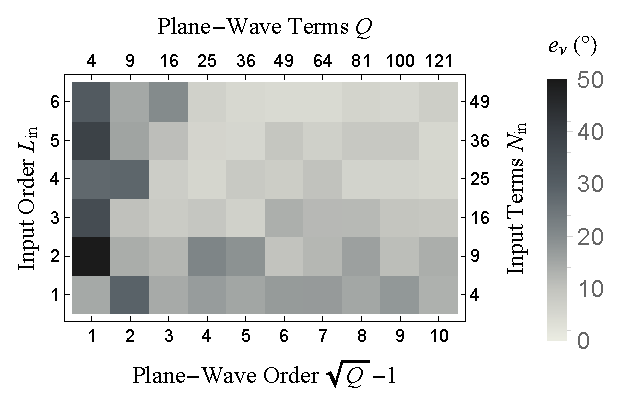
\includegraphics[width=\textwidth]{07_characterization_extrapolation/figures/tylka2017_order_pwt-pinv.eps}
        		\caption{Localization error $e_\nu$ -- pseudoinversion}
        		\label{fig:07_Characterization_Extrapolation:Localization_Order:PWT-pinv}
    	\end{subfigure}
	
	\vspace{0.5cm}
	\begin{subfigure}[b]{0.49\textwidth}
        		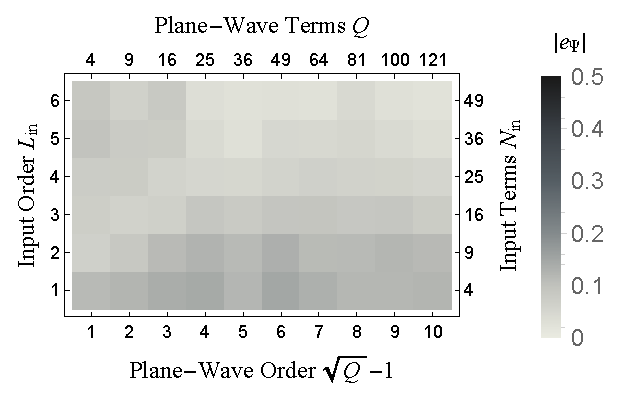
\includegraphics[width=\textwidth]{07_characterization_extrapolation/figures/merimaa2005_d_order_pwt-bf.eps}
        		\caption{Diffuseness error $e_\Psi$ -- beamforming}
        		\label{fig:07_Characterization_Extrapolation:Diffuseness_Order:PWT-bf}
    	\end{subfigure}
	\hfill
    	\begin{subfigure}[b]{0.49\textwidth}
        		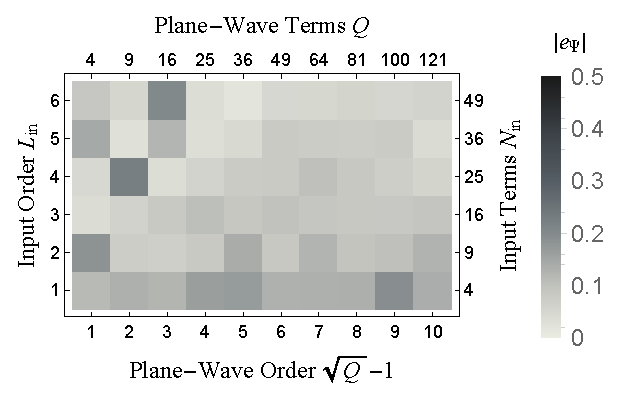
\includegraphics[width=\textwidth]{07_characterization_extrapolation/figures/merimaa2005_d_order_pwt-pinv.eps}
        		\caption{Diffuseness error $e_\Psi$ -- pseudoinversion}
        		\label{fig:07_Characterization_Extrapolation:Diffuseness_Order:PWT-pinv}
    	\end{subfigure}
	
    	\caption[]{Dependence of errors on $Q$ and ambisonics input order $L_\text{in}$ (continued from p.~\pageref{fig:07_Characterization_Extrapolation:PWT_Order_Dependence}).}
    	\label{fig:07_Characterization_Extrapolation:PWT_Order_Dependence:contd}
\end{figure*}

From the diffuseness errors (see \secref{sec:04_Auditory_Models:Diffuseness_Parameter}) plotted in \figref{fig:07_Characterization_Extrapolation:Diffuseness_Order:PWT-bf}, we see that the beamforming method only yields relatively large errors at low ambisonics orders, e.g., $L_\text{in} = 1,2$.
For the pseudoinversion method, however, we again see a sensitivity to mismatched sampling conditions, yielding relatively large errors without any discernible pattern.
Consequently, unless the plane-wave terms can be carefully chosen ahead of time for a given ambisonics order, beamforming is likely the safer method.

\section{Source azimuth dependence}\label{sec:07_Characterization_Extrapolation:Azimuth_Dependence}
In this section, we examine the effective frequency response induced by translation via each method as a function of source azimuth.
As described in \secref{sec:06_Simulation_Framework:Azimuth_Dependence}, for these simulations, we let $L_\text{in} = 4$, pick $u = 0.25$~m and $s_0 = 2.5$~m (so $\gamma = 10$), and translate to $\vec{r}_0 = (0, 0, 0)$.
Based on the findings discussed above, here we use beamforming with $Q = N_\text{in} = 25$ for the plane-wave translation method.

The induced frequency responses are plotted in \figref{fig:07_Characterization_Extrapolation:Azimuth_Dependence}.
From \figref{fig:07_Characterization_Extrapolation:Azimuth_Dependence:PWT}, we see that the plane-wave translation method introduces sporadic notches in the frequency response of the signal, which do not appear to follow any obvious pattern.
Otherwise, however, the frequency responses are largely flat for all source azimuths.
This is in agreement with the finding of \citet[cf.~Figs.~7c and 7f]{HahnSpors2015b}: that the induced frequency responses are largely flat under critically-sampled conditions, i.e., when the number of plane-wave terms matches the number of ambisonics signals.

\begin{figure*}[t]
    	\centering
    	\begin{subfigure}[b]{0.49\textwidth}
        		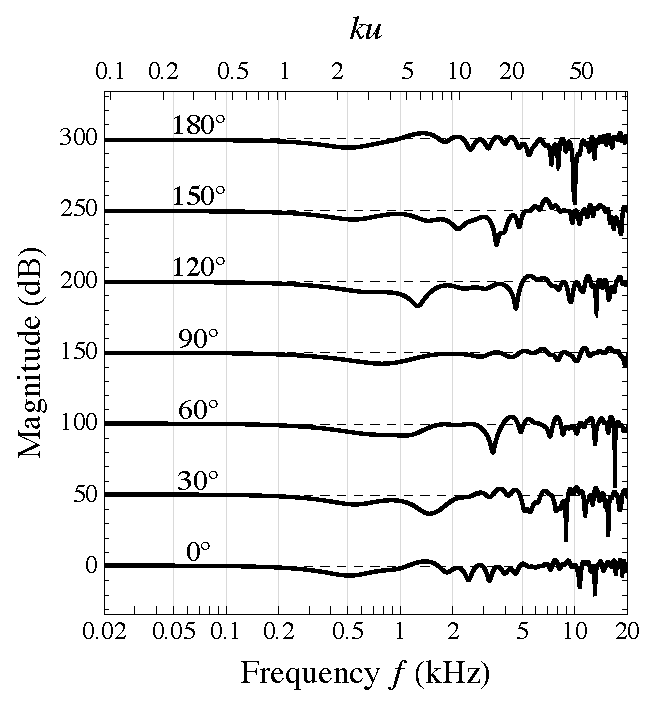
\includegraphics[width=\textwidth]{07_characterization_extrapolation/figures/sourceAz_freqResp_pwt.eps}
        		\caption{Plane-wave translation}
        		\label{fig:07_Characterization_Extrapolation:Azimuth_Dependence:PWT}
    	\end{subfigure}
	\hfill
    	\begin{subfigure}[b]{0.49\textwidth}
        		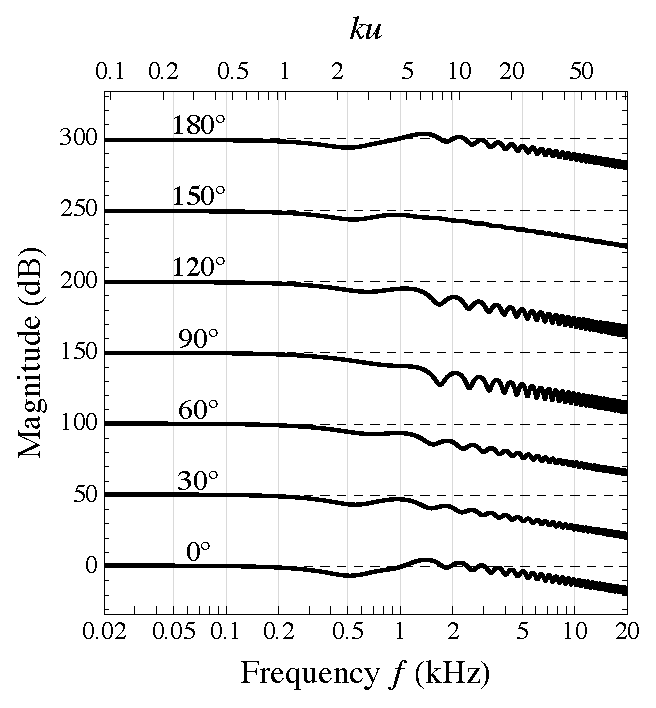
\includegraphics[width=\textwidth]{07_characterization_extrapolation/figures/sourceAz_freqResp_sre.eps}
        		\caption{Ambisonics translation}
        		\label{fig:07_Characterization_Extrapolation:Azimuth_Dependence:SRE}
    	\end{subfigure}
	
	\caption[Magnitude responses across azimuths for each extrapolation method.]{
	Magnitude responses caused by the plane-wave and ambisonics translation methods for various source azimuths.
  The bottom axes show frequency in kHz while the top axes show the nondimensional frequency $ku$ for a microphone distance of $u = 0.25$~m.
  For legibility, each frequency response is offset by $50$~dB and the responses have been artificially truncated (where needed) to not exceed $-45$~dB.}
	\label{fig:07_Characterization_Extrapolation:Azimuth_Dependence}
\end{figure*} %%NOTE%% vertical axis label is too complicated: |A0 / B0ref| or something

We also note from \figref{fig:07_Characterization_Extrapolation:Azimuth_Dependence:PWT} that the frequency response for a source azimuth of $90^\circ$ is particularly flat, which suggests that translation perpendicular to the direction of the source introduces very little spectral coloration.
This appears to contradict another finding of \citet{HahnSpors2015b}: that translation parallel to the source direction introduces less coloration than translation perpendicularly.
However, their finding was only shown for oversampled conditions, where $Q > N_\text{in}$ \citep[cf.~Fig.~7]{HahnSpors2015b}; for critically-sampled conditions (where $Q = N_\text{in}$), as considered here, the induced coloration is apparently smaller (albeit not nearly as significantly so) for perpendicular translations.

As shown in \figref{fig:07_Characterization_Extrapolation:Azimuth_Dependence:SRE}, the ambisonics translation method introduces a high-frequency roll-off, which does not depend on source azimuth.
Recall from \secref{sec:03_Navigation_Techniques:SR_Technique}, however, that the corner frequency of this roll-off does vary proportionally to $L_\text{in} / \| \vec{r}_0 - \vec{u} \|$.
Consequently, we expect the spectral coloration induced by this method to increase steadily with increasing translation distance, while the overall level will steadily decrease.

\section{Characterization and discussion}\label{sec:07_Characterization_Extrapolation:Results}
Based on our findings in \secref{sec:07_Characterization_Extrapolation:Plane-wave_Dependence}, we use beamforming with $Q = N_\text{in}$ for the plane-wave translation method in all simulations discussed below.

% Level

Level error contour plots are shown in the top panels of \figref{fig:07_Characterization_Extrapolation:Level_Spectral_Errors}.
For the plane-wave translation method (see \figref{fig:07_Characterization_Extrapolation:Level_Errors:PWT}), we see that exterior sources experience negligible level error;
interior sources, however, are reproduced approximately $6$~dB too quietly for most microphone distances.
For the ambisonics translation method (see \figref{fig:07_Characterization_Extrapolation:Level_Errors:SRE}), we see a general trend of increasing level error with microphone distance at all source distances, although exterior sources consistently experience less severe level errors than interior ones for the same $u$, and at very large $u$ and $\gamma$ (top right corner of \figref{fig:07_Characterization_Extrapolation:Level_Errors:SRE}), the errors become less severe.
The degradation in performance with increasing microphone distance is due to the high-frequency roll-off induced by the ambisonics translation filters, as discussed in \secref{sec:07_Characterization_Extrapolation:Azimuth_Dependence}, which yields a decrease in overall level.
Taken together, these results imply that a violation of the region of validity restriction (i.e., for interior sources) tends to yield a reproduced level that is significantly too low. % overall, exterior is much better; violating region of validity --> too quiet

\begin{figure*}[tbp]
    	\centering
    	\begin{subfigure}[b]{0.49\textwidth}
        		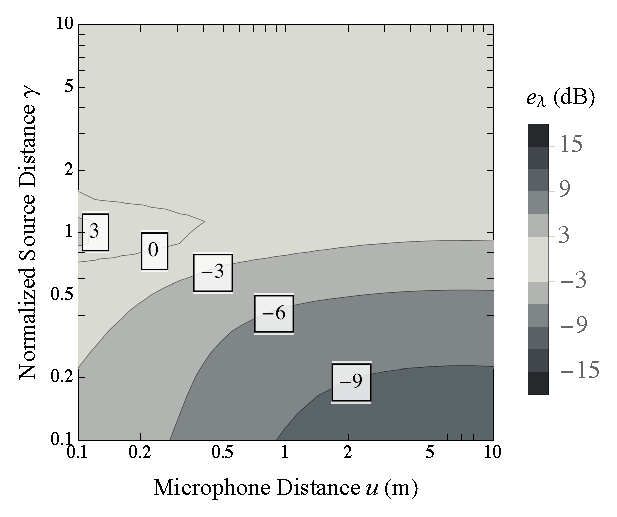
\includegraphics[width=\textwidth]{07_characterization_extrapolation/figures/audibleEnergy_contour_pwt.eps}
        		\caption{$e_\lambda$ -- plane-wave translation}
        		\label{fig:07_Characterization_Extrapolation:Level_Errors:PWT}
    	\end{subfigure}
	\hfill
    	\begin{subfigure}[b]{0.49\textwidth}
        		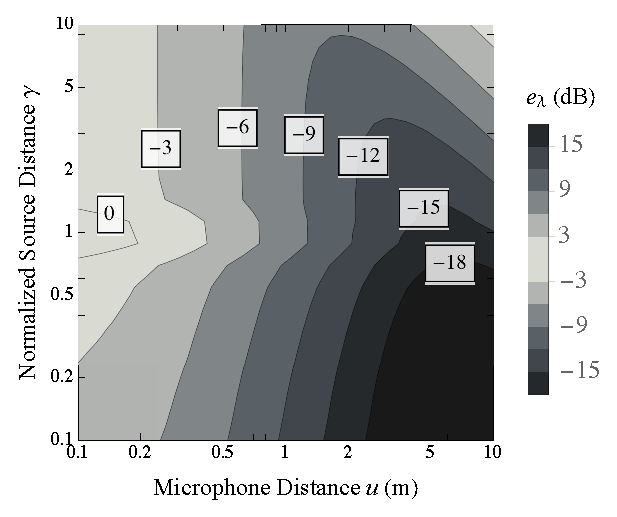
\includegraphics[width=\textwidth]{07_characterization_extrapolation/figures/audibleEnergy_contour_sre.eps}
        		\caption{$e_\lambda$ -- ambisonics translation}
        		\label{fig:07_Characterization_Extrapolation:Level_Errors:SRE}
    	\end{subfigure}
	
	\vspace{0.5cm}
	\begin{subfigure}[b]{0.49\textwidth}
        		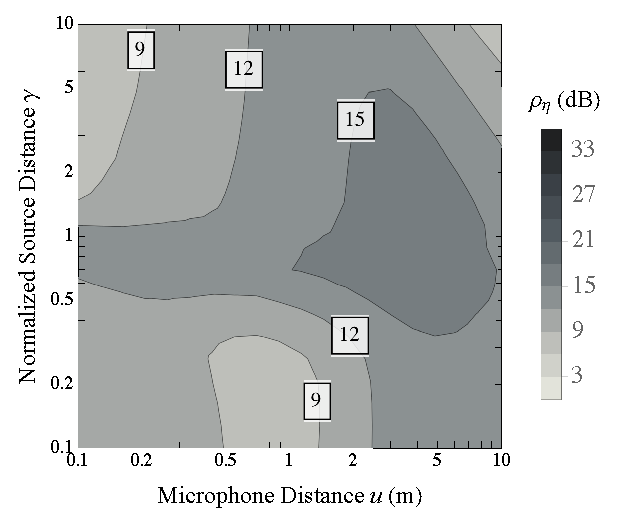
\includegraphics[width=\textwidth]{07_characterization_extrapolation/figures/scharer2009_contour_pwt.eps}
        		\caption{$\rho_\eta$ -- plane-wave translation}
        		\label{fig:07_Characterization_Extrapolation:Spectral_Errors:PWT}
    	\end{subfigure}
	\hfill
    	\begin{subfigure}[b]{0.49\textwidth}
        		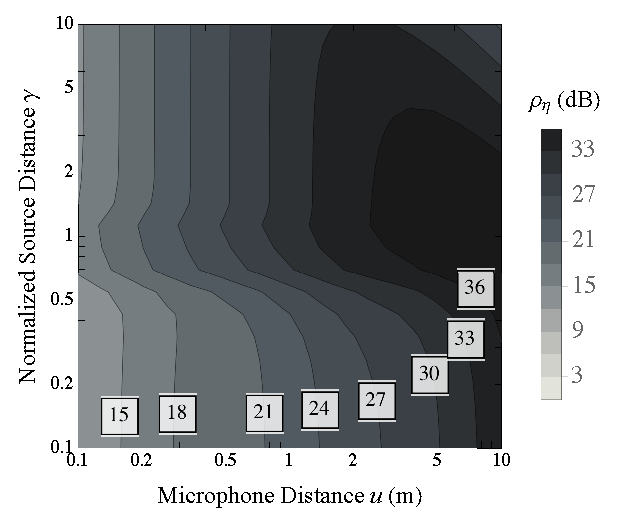
\includegraphics[width=\textwidth]{07_characterization_extrapolation/figures/scharer2009_contour_sre.eps}
        		\caption{$\rho_\eta$ -- ambisonics translation}
        		\label{fig:07_Characterization_Extrapolation:Spectral_Errors:SRE}
    	\end{subfigure}
	
    	\caption[Level and coloration contour plots for each extrapolation method.]{
	Level errors $e_\lambda$ (top panels) and spectral errors $\rho_\eta$ (bottom) for microphone distance $u$ and normalized source distance $\gamma$.
  Contour lines are drawn every $3$~dB.}
    	\label{fig:07_Characterization_Extrapolation:Level_Spectral_Errors}
\end{figure*}

% Coloration

In the bottom panels of \figref{fig:07_Characterization_Extrapolation:Level_Spectral_Errors}, we plot the spectral errors incurred by both methods.
The plane-wave translation method does not appear to exhibit any clear trend (see \figref{fig:07_Characterization_Extrapolation:Spectral_Errors:PWT}), although we do see that, for any given microphone distance, the greatest spectral errors occur for source distances around $\gamma = 1$.
Furthermore, this method tends to experience the largest spectral error ($\rho_\eta > 15$~dB) at large microphone distances ($u > 1$~m) with $\gamma \sim 1$.
Additionally, there are two regions of low error: 1) at very small microphone distances with very far-field sources (top left corner of \figref{fig:07_Characterization_Extrapolation:Spectral_Errors:PWT}) and 2) for microphone distances around $u \approx 1$~m with far interior sources ($\gamma < 0.3$).

As shown in \figref{fig:07_Characterization_Extrapolation:Spectral_Errors:SRE}, the ambisonics translation method exhibits similar behavior in terms of spectral error as it does for level errors:
in this plot, we again see a clear trend of increasing error with microphone distance (again due to the high-frequency roll-off), with the exception of a region of slightly less severe errors at very large $u$ and $\gamma$.
However, in this case, interior sources experience approximately $6$~dB less spectral error than corresponding exterior ones (for a fixed $u$).

% Localization

From \figref{fig:07_Characterization_Extrapolation:Localization_Errors:PWT}, we see that the plane-wave translation method introduces very small localization errors for exterior sources.
This is somewhat intuitive, since as $\gamma$ increases, the source appears more like a plane-wave source, which should be natural to reproduce using the plane-wave translation method.
The ambisonics translation method, however, is only accurate at very small microphone distances with very far exterior sources (as shown in the top left corner of \figref{fig:07_Characterization_Extrapolation:Localization_Errors:SRE}).
Otherwise, for exterior sources, the errors incurred by the ambisonics translation method increase steadily with increasing microphone distance.
Additionally, both methods yield large errors at all microphone distances for interior sources with approximately $0.3 < \gamma < 1$, as well as at very small $u$ and $\gamma$ (bottom left corners of both \figreftwo{fig:07_Characterization_Extrapolation:Localization_Errors:PWT}{fig:07_Characterization_Extrapolation:Localization_Errors:SRE}).
That this behavior is common to both methods implies that it is the violation of the region of validity restriction which causes these extremely large localization errors. % the band of large errors as well as the bottom left corner are common to both --> inherent to region of validity violation

\begin{figure*}[tbp]
    	\centering
    	\begin{subfigure}[b]{0.49\textwidth}
        		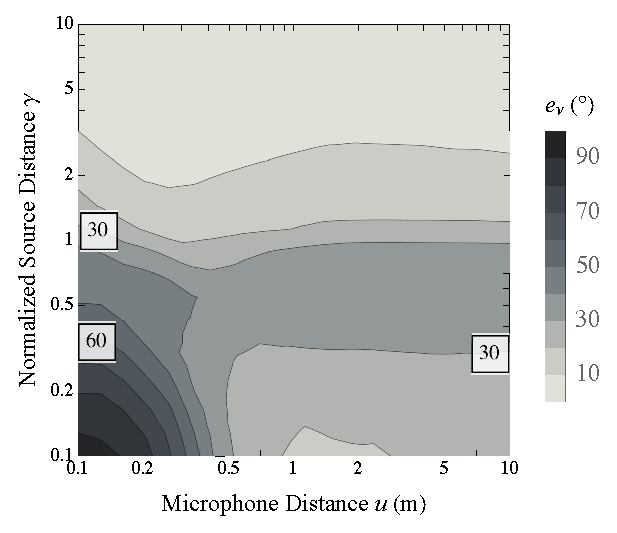
\includegraphics[width=\textwidth]{07_characterization_extrapolation/figures/tylka2017_contour_pwt.eps}
        		\caption{$e_\nu$ -- plane-wave translation}
        		\label{fig:07_Characterization_Extrapolation:Localization_Errors:PWT}
    	\end{subfigure}
	\hfill
    	\begin{subfigure}[b]{0.49\textwidth}
        		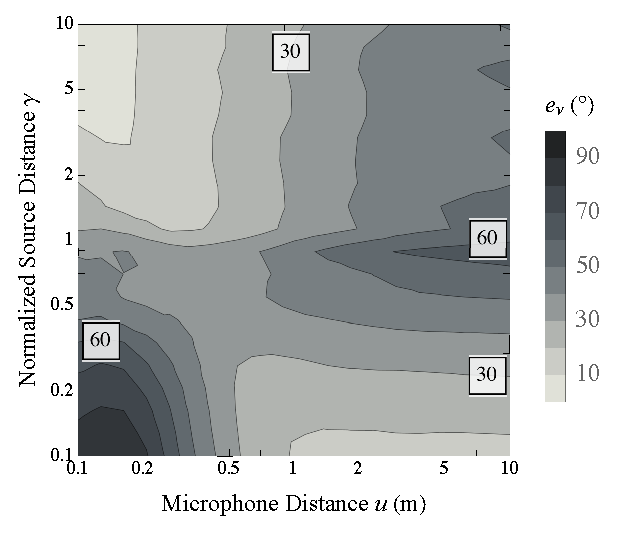
\includegraphics[width=\textwidth]{07_characterization_extrapolation/figures/tylka2017_contour_sre.eps}
        		\caption{$e_\nu$ -- ambisonics translation}
        		\label{fig:07_Characterization_Extrapolation:Localization_Errors:SRE}
    	\end{subfigure}
	
	\vspace{0.5cm}
	\begin{subfigure}[b]{0.49\textwidth}
        		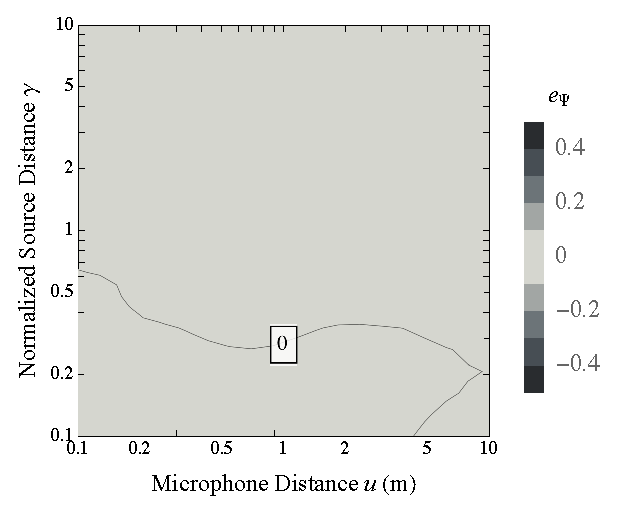
\includegraphics[width=\textwidth]{07_characterization_extrapolation/figures/merimaa2005_d_contour_pwt.eps}
        		\caption{$e_\Psi$ -- plane-wave translation}
        		\label{fig:07_Characterization_Extrapolation:Diffuseness_Errors:PWT}
    	\end{subfigure}
	\hfill
    	\begin{subfigure}[b]{0.49\textwidth}
        		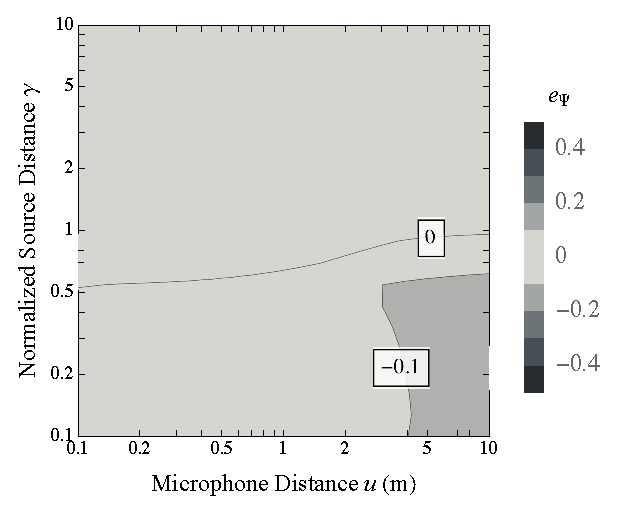
\includegraphics[width=\textwidth]{07_characterization_extrapolation/figures/merimaa2005_d_contour_sre.eps}
        		\caption{$e_\Psi$ -- ambisonics translation}
        		\label{fig:07_Characterization_Extrapolation:Diffuseness_Errors:SRE}
    	\end{subfigure}
	
    	\caption[Localization and diffuseness contour plots for each extrapolation method.]{
	Localization errors $e_\nu$ (top panels) and diffuseness errors $e_\Psi$ (bottom) for microphone distance $u$ and normalized source distance $\gamma$.
  Localization error contour lines are drawn every $10^\circ$; diffuseness error contour lines are drawn in increments of $0.1$.}
    	\label{fig:07_Characterization_Extrapolation:Localization_Diffuseness_Errors}
\end{figure*}

% Diffuseness

As shown in the bottom panels of \figref{fig:07_Characterization_Extrapolation:Localization_Diffuseness_Errors}, both methods achieve nearly zero diffuseness errors, although the ambisonics translation method exhibits a region of minor errors ($e_\Psi \approx -0.1$) for interior sources at large microphone distances (bottom right corner of \figref{fig:07_Characterization_Extrapolation:Diffuseness_Errors:SRE}).

%% Order Dependence %%
\subsection{Order dependence}
In \figref{fig:07_Characterization_Extrapolation:Order_Errors}, we plot errors for each metric and for both methods as functions of microphone distance $u$ for a fixed source distance of $s_0 = 1$~m and for several input ambisonics orders $L_\text{in}$ (with matching $Q = N_\text{in} = (L_\text{in} + 1)^2$ for the plane-wave translation method).

From \figref{fig:07_Characterization_Extrapolation:Level_Errors:Order}, we see that, in terms of level errors, increasing the ambisonics input order tends to improve performance, albeit only marginally.
Additionally, the performance of both methods degrades with increasing microphone distance, with exterior sources (where $u < s_0 = 1$~m) exhibiting significantly less severe errors than interior ones (where $u > s_0$).
Furthermore, all of these curves exhibit a ``knee'' at $u = 1$~m, where the curves experience a qualitative change in behavior.
In particular, the plane-wave translation method exhibits two distinct regimes on either side of $u = 1$~m: for exterior sources, the method incurs constant level errors, whereas for interior sources, the errors grow more extreme with increasing $u$.
For the ambisonics translation method, increasing $u$ tends to produce more extreme errors overall, and the errors grow more rapidly in the interior source regime than in the exterior source regime.
Only the plane-wave translation method with exterior sources exhibits negligible level errors ($\sim1$~dB), which is a consequence of our choice to match the number of plane-wave terms, $Q$, to the number of ambisonics signals, $N_\text{in} = (L_\text{in} + 1)^2$.

\begin{figure*}[t]
    	\centering
	\begin{subfigure}[b]{0.49\textwidth}
        		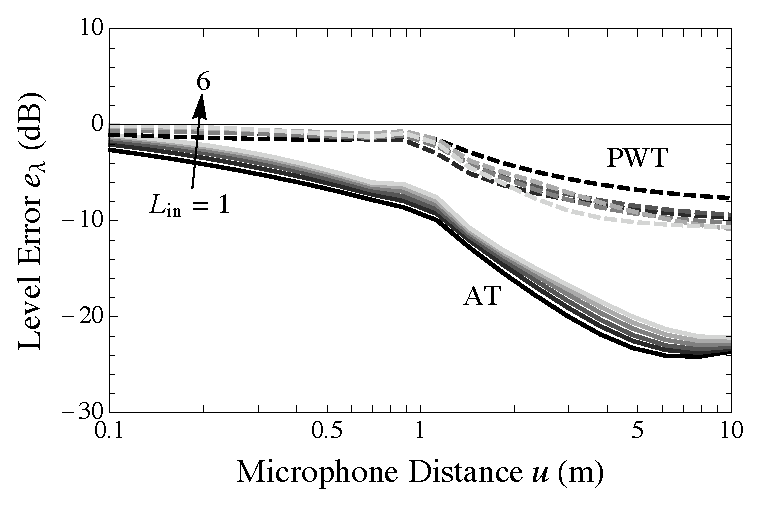
\includegraphics[width=\textwidth]{07_characterization_extrapolation/figures/audibleEnergy_order.eps}
        		\caption{Level errors $e_\lambda$}
        		\label{fig:07_Characterization_Extrapolation:Level_Errors:Order}
    	\end{subfigure}
	\hfill
    	\begin{subfigure}[b]{0.49\textwidth}
        		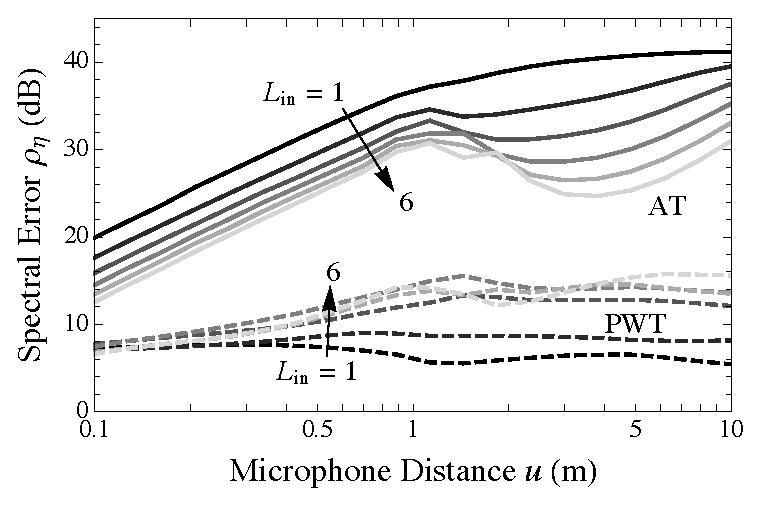
\includegraphics[width=\textwidth]{07_characterization_extrapolation/figures/scharer2009_order.eps}
        		\caption{Spectral errors $\rho_\eta$}
        		\label{fig:07_Characterization_Extrapolation:Spectral_Errors:Order}
    	\end{subfigure}
	
	\vspace{0.5cm}
	\begin{subfigure}[b]{0.49\textwidth}
        		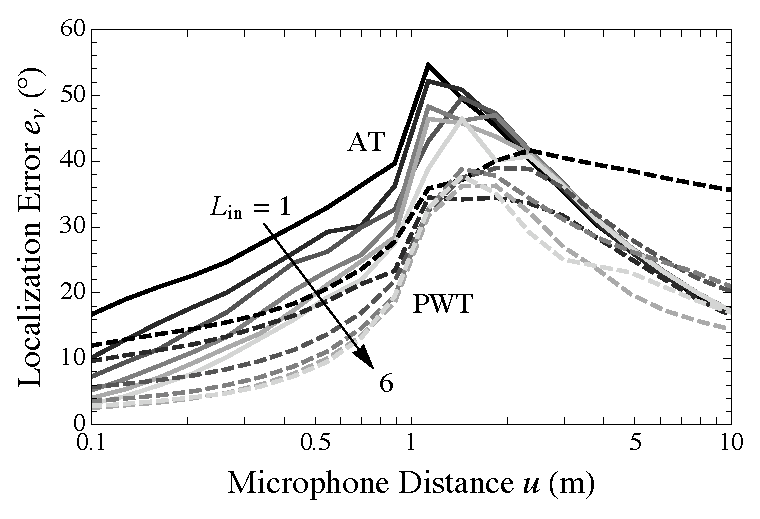
\includegraphics[width=\textwidth]{07_characterization_extrapolation/figures/tylka2017_order.eps}
        		\caption{Localization errors $e_\nu$}
		\label{fig:07_Characterization_Extrapolation:Localization_Errors:Order}
    	\end{subfigure}
	\hfill
    	\begin{subfigure}[b]{0.49\textwidth}
        		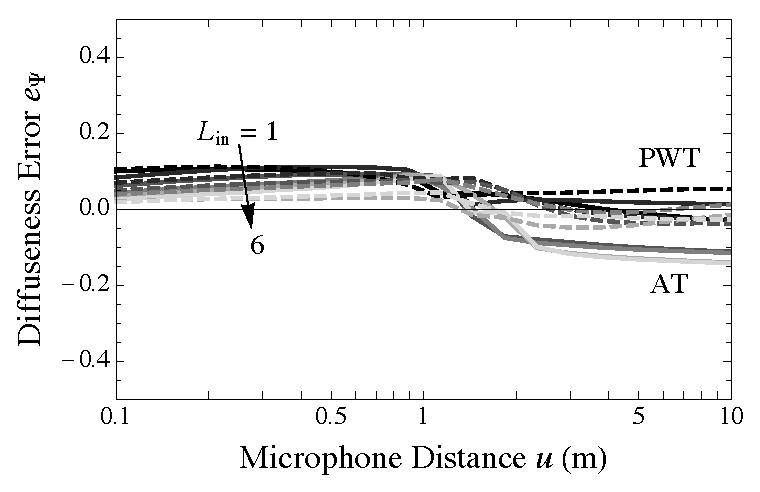
\includegraphics[width=\textwidth]{07_characterization_extrapolation/figures/merimaa2005_d_order.eps}
        		\caption{Diffuseness errors $e_\Psi$}
		\label{fig:07_Characterization_Extrapolation:Diffuseness_Errors:Order}
    	\end{subfigure}
	
    	\caption[Order dependence plots for each extrapolation method.]{
	Errors for various microphone distances $u$ with a fixed source distance $s_0 = 1$~m.
	Errors are plotted for the ambisonics translation method (solid curves, labeled ``AT'') and the plane-wave translation method (dashed curves, labeled ``PWT'').
	For each method, six input ambisonics orders are shown: $L_\textrm{in} = 1$ (black) to $L_\textrm{in} = 6$ (lightest gray).}
    	\label{fig:07_Characterization_Extrapolation:Order_Errors}
\end{figure*}

From \figref{fig:07_Characterization_Extrapolation:Spectral_Errors:Order}, we again see that increasing the ambisonics order $L_\text{in}$ yields an improvement in performance (i.e., a decrease in spectral errors) for the ambisonics translation method.
Here again we note two distinct regimes for this method on either side of $u = 1$~m with a transition region where the behavior changes.
Additionally, within each regime, the errors again increase monotonically with increasing $u$.
However, unlike with level errors, we now see a more rapid (but still monotonic) increase in error for \textit{exterior} sources ($u < 1$~m), while the more gradual performance degradation occurs for \textit{interior} sources ($u > 1$~m).
For the plane-wave translation method, we see that increasing $L_\text{in}$ yields an \textit{increase} in spectral error, and that this increase in error is more severe for interior sources than for exterior ones.
This suggests a penalty from violating the region of validity restriction that is particular to the plane-wave translation method: that a larger ambisonics input order incurs more spectral coloration.

As shown in \figref{fig:07_Characterization_Extrapolation:Localization_Errors:Order}, the localization errors for both methods tend to improve with increasing $L_\text{in}$, and the existence of two regimes on either side of $u = 1$~m is evident.
For exterior sources ($u < 1$~m), the errors improve with decreasing $u$, whereas for interior sources ($u > 1$~m), the opposite is true: the errors improve with \textit{increasing} $u$.
Evidently, a microphone distance of $u \approx s_0$ (i.e., $\gamma \approx 1$) yields the most extreme errors.
Overall, the ambisonics translation method tends to perform worse than the plane-wave translation method (except at very large $u$ and $L_\text{in} = 1$) and the errors for both methods are typically smaller for exterior sources than for interior ones.

It is worth noting that by construction, since $s_0$ is fixed, as $u$ increases beyond $1$~m, more of the navigable region (see \figref{fig:06_Simulation_Framework:Point_Geometry}) becomes valid for translation.
For instance, with $u = 10$~m and $s_0 = 1$~m, the listener can navigate approximately $9$~m away from the microphone and still remain inside its region of validity.
This explains in part the improvement with increasing $u$ seen for $u > 1$~m, since, on average, more of the navigable region is valid.
That is, when averaging errors over the entire navigable region, a smaller fraction of that region will actually be in violation of the region of validity restriction.

Finally, as shown in \figref{fig:07_Characterization_Extrapolation:Diffuseness_Errors:Order}, both methods achieve small diffuseness errors, and generally, increasing $L_\text{in}$ improves the performance for exterior sources.
Again we see a transition between regimes occurring at $u \approx 1$~m.

\section{Conclusions}\label{sec:07_Characterization_Extrapolation:Conclusions}
In this chapter, we presented the results of numerical simulations conducted in order to characterize and compare the performance of the plane-wave and ambisonics translation methods.
Following the simulation framework laid out in \chapref{chap:06_Simulation_Framework}, we simulated simple incident sound fields consisting of a single microphone and a single point-source, varying source distance and azimuth, as well as microphone distance and listener position.
First, in \secref{sec:07_Characterization_Extrapolation:Plane-wave_Dependence}, we determined suitable parameters for the plane-wave translation method, comparing the beamforming and pseudoinversion methods for computing the plane-wave decomposition and varying both the ambisonics input order and the number of plane-wave terms.
We then explored, in \secref{sec:07_Characterization_Extrapolation:Azimuth_Dependence}, basic properties of each method by computing the effective frequency responses induced by the plane-wave and ambisonics translation methods across source azimuths.
Finally, in \secref{sec:07_Characterization_Extrapolation:Results}, we conducted a more comprehensive analysis of both methods in terms of the metrics enumerated in \secref{sec:06_Simulation_Framework:Metrics} for sound level, spectral coloration, source localization, and diffuseness.

The analyses presented in this chapter yielded the following major findings:
\begin{itemize}
\item for the plane-wave translation method, a clear advantage exists to using the beamforming plane-wave decomposition method (see \eqnref{eq:02_Acoustical_Theory:A2mu}) and matching the number of ambisonics signals, $N$, to the number of plane-wave terms, $Q$;%
\footnote{All subsequent findings relate to this implementation of the plane-wave translation method: beamforming with matched $Q = N$.}
%\item the pseudoinversion plane-wave decomposition method (see \eqnref{eq:02_Acoustical_Theory:A2mu_Pinv}) exhibited a similar advantage, as well as an advantage to ``oversampling'' directions by taking $Q > N$, although this method also appeared more sensitive to mismatches than the beamforming method;
\item the frequency responses induced by the plane-wave translation method are largely flat but with sporadic notches while those induced by the ambisonics translation method exhibit a consistent low-pass-like roll-off of high-frequency energy, but both methods appear largely insensitive to source azimuth;
\item the ambisonics translation method incurs significant errors in both level and coloration at all source distances which, overall, increase steadily with microphone distance;
\item for exterior sources, the plane-wave translation method achieves a high degree of accuracy in both level and localization;
\item for interior sources, where the region of validity restriction is violated, both methods incur significant errors in both level and localization; and
\item more generally, both methods tend to exhibit two distinct regimes of behavior for exterior and interior sources, with a transition region between the two, and the performance for interior sources is often degraded compared to that for exterior sources.
\end{itemize}
Additionally, results showed that increasing the ambisonics order tends to uniformly improve the performance of both methods, with the exception of the spectral errors incurred by the plane-wave translation method.

Due to the extremely large level and coloration errors incurred by the ambisonics translation method, the plane-wave translation method is likely the only viable method for most applications with practical translation distances (e.g., $u > 0.5$~m).
This method is particularly well-suited for exterior sources, but its performance degrades significantly, in terms of localization in particular, once the region of validity restriction is violated.
The remaining challenge for this method is the introduction of significant spectral errors ($\rho_\eta > 10$~dB) over all microphone and source distances.
Consequently, future improvements to this method should attempt to correct this coloration, perhaps parametrically based on source direction.

As demonstrated in this chapter, the performance of linear extrapolation-based navigational methods is significantly impaired by the presence of near-field sources.
Consequently, parametric and interpolation-based approaches have been developed that aim to extend navigation beyond such near-field sources while maintaining acceptable performance.
In the following chapters, we characterize and compare the performance of several such methods:
in \chapref{chap:08_Proposed_Method}, we propose a parametric interpolation method and demonstrate its improvement over a benchmark linear interpolation method and,
in \chapref{chap:09_Thiergart_Comparison}, we perform a similar analysis of an existing parametric interpolation method.

\section*{Acknowledgements}
This work is a significantly updated version of a paper originally presented by \citet{TylkaChoueiri2015} at the 139\textsuperscript{th} Convention of the Audio Engineering Society.
The analysis presented here was originally submitted by \citet{TylkaChoueiri2019c} to \textit{The Journal of the Audio Engineering Society}.
%%%% COMPARISON TO WEIGHTED AVERAGE METHOD %%%%
\chapter{Parametric exclusion of invalid microphones and comparison to weighted-average interpolation}\label{chap:08_Proposed_Method}
In this chapter, we propose an interpolation-based method for virtual navigation, wherein the subset of microphones to be used is parametrically determined to ensure that the region of validity restriction is not violated.
We take an existing, weighted-average-based navigational method as a benchmark due to its simplicity and its applicability to arbitrary sound fields, and present a comprehensive characterization and comparison of the performance of both methods following the numerical simulation framework laid out in \chapref{chap:06_Simulation_Framework}.
Through these analyses, we aim to demonstrate the improvement in performance achieved by the proposed method (compared to the benchmark) and, in particular, explore the penalties incurred by the benchmark method when the region of validity restriction is violated.

\section{Introduction}\label{sec:08_Proposed_Method:Introduction}
As shown in the previous chapter, existing methods for sound field navigation using a single ambisonics microphone tend to introduce significant errors in the reproduced level, spectral coloration, and source localization, even over relatively small translation distances (see \secref{sec:07_Characterization_Extrapolation:Results}).
This is a consequence of the well-established limitation of the ambisonics framework: that a finite-order expansion of a sound field yields only an approximation to that sound field, the accuracy of which decreases with increasing frequency and distance from the expansion center \citep{Poletti2005,WardAbhayapala2001} (see \eqnref{eq:01_Introduction:kr_Inequality})
As was also shown in that chapter, the performance of these extrapolation methods is often significantly degraded when the listener navigates beyond the distance of that source from the microphone.
In particular, we showed that this violation of the region of validity restriction (discussed in \secref{sec:02_Acoustical_Theory:Helmholtz_Equation}) causes both of the methods considered in that chapter to incur significant errors in the reproduced levels and localization of the sources.

In an effort to overcome these challenges, several previous studies have developed navigational methods that employ an array of ambisonics microphones distributed throughout the sound field (or, equivalently, encode a synthetic sound field into ambisonics at multiple discrete positions).
In the following section, we provide a critical review of these existing methods and identify the main challenges they face.
All of the methods discussed below are listed in \tabref{tab:01_Introduction:Methods}.
%These methods typically involve either some form of interpolation between the microphones or an analysis of the incident sound field followed by a reconstruction of a simplified model of that sound field.
%Ideally, such methods should enable virtual navigation of any arbitrary sound field consisting of arbitrary signals without introducing spectral coloration or audible processing artifacts.
%Additionally, they should achieve accurate sound localization even in the vicinity of near-field sources.
%In the following section, we review existing methods for sound field navigation that employ multiple spatially-distinct ambisonics microphones, and discuss their deficiencies.

%%%% Previous Work %%%%
% Review of previous work focusing on the remaining problems (questions or deficiencies) the present paper claims to contribute to solving
\subsection{Previous work}
Perhaps the simplest interpolation-based navigational method is to compute a per-channel weighted average of the ambisonics signals from each microphone, where the interpolation weights are related to the distances from the listener to each microphone (see \secref{sec:03_Navigation_Techniques:XF_Technique}).
This approach has been implemented by \citet{MarietteKatz2009} using virtual first-order ambisonics (FOA) microphones spaced $20$~m apart and arranged in both linear (two microphones) and triangular (three microphones) configurations.
Similarly, \citet{Southern2009} employed this method in order to interpolate ambisonics room impulse responses (RIRs) to enable real-time navigable auralizations of acoustic spaces.
% In their study, \citeauthor{Southern2009} interpolate between RIR measurements spaced $5.5$~m apart, but only consider a symmetric source position.

One fundamental limitation of this method is that it necessarily confines the listener to the region interior to the microphone array, since it is purely an interpolation method with no means of extrapolation.
Additionally, this method can violate the region of validity restriction mentioned above, since even those microphones that are nearer to a source than to the desired listening position are included in the calculation.
As we will show in the present chapter, such a violation leads to a degradation of the estimated sound field at the listening position.
Furthermore, objective and perceptual investigations have shown that this method suffers from significant localization errors, in particular when the source distance (from the center of the microphone array) is small compared to the microphone spacing \citep{MarietteKatz2009,Mariette2010} (here, we refer to this condition as having an ``interior source'').
This effect is consistent with findings from a previous study of ours \citep[Fig.~6]{TylkaChoueiri2016}.
In that study, we also showed that if a sound source is nearer to one microphone than to another (as is the case for most source directions), this method will necessarily induce comb-filtering \citep[Fig.~4a]{TylkaChoueiri2016}.
This is to be expected: each microphone captures essentially the same signals, separated by a finite time delay, so the signals will interfere constructively or destructively when summed, depending on frequency, due to the phase shift between them.
In \secref{sec:08_Proposed_Method:Fundamental_Problems}, we revise and expand these analyses.

\citet{Patricio2019} introduced and experimentally demonstrated a distance-biased linear interpolation method in which the directional components of the microphone nearest to the listener are emphasized over those of the farther microphones.
The method also employs a low-pass filter on each microphone's signals to mimic the atmospheric absorption of high frequencies.
Fundamentally, this method is subject to the same issues and limitations as the weighted average method, since it is essentially the same calculation but with a particular (order- and frequency-dependent) prescription for the interpolation weights.
While it is plausible that the adopted biasing approach may mitigate the localization errors incurred by the weighted average method, this remains to be seen since the two methods have not yet been compared.

Recently, \citet{Emura2017} proposed a method for two ambisonics microphones which combines the measured signals in order to estimate coefficients for a single global plane-wave decomposition of the sound field.
In this method, a so-called ``dictionary'' matrix is pre-computed for a high-resolution grid of plane-waves incident on the microphones, and the plane-wave signals that best explain the measured pressures on the microphones are determined.
This method, based on compressed sensing techniques (which have been reviewed by \citet{Epain2009} in the context of spatial sound field analysis and synthesis), entails minimizing the $\ell_1$ norm of an error signal \citep[see Eq.~(20)]{Emura2017} and is consequently nonlinear with respect to the measured signals.
The evaluation of this method presented by the authors is limited to low-frequency rms error calculations, which show that the performance of the method is improved in the vicinity of the second microphone compared to if only a single microphone is used. % probably just because of the second mic; not necessarily due to the method
However, due to the plane-wave-based nature of the proposed method, it can be expected that near-field and interior sources will be problematic.

\citet{Bates2018} developed a perceptually-motivated method for sound field navigation using a $50$~cm $\times$ $50$~cm square arrangement of four FOA microphones.%
\footnote{This work extends the so-called ``perspective control microphone array'' method, which creates the perception of navigation by varying the mixing of the signals from 5 coincident pairs of microphones (cardioid and hypercardioid), spaced $\sim2$~m apart \citep{Lee2011,Lee2012}.}
In this method, each ambisonics microphone is used to create a virtual directional microphone, the placement and directivity of which are varied as a function of listener position.
The signals from these virtual directional microphones are then encoded into a single ambisonics stream.
Based on its formulation, this method appears well-suited for applications with a small, predefined navigable region, but would be difficult to extend to cover a larger region.
Additionally, in an objective analysis of perceived source distance and direction, this method achieved promising performance when navigating towards the source, but yielded significant directional errors and diminished distance performance when navigating away \citep[section 3]{Bates2018}.

In the context of ambisonics RIR interpolation, the issues of comb-filtering and localization errors may be mitigated by taking a dynamic time warping approach, similar to that proposed by \citet{Masterson2009}.
% if this were a review paper, explain what DTW is
Although this approach has not been implemented to interpolate ambisonics RIRs specifically, a previous study by the same authors has suggested incorporating arbitrary microphone directivity \citep{Kearney2009}, which would enable extending this method to ambisonics.%
\footnote{More recently, \citet{GarciaGomezLopez2018} extended this method to interpolate binaural RIRs.}
One limitation of this method is that it requires knowledge not only of the microphone positions, but also of the source position, which, for an arbitrary sound field, would not be known \textit{a priori}.
Consequently, this method might be improved by incorporating some basic source localization algorithm, for example, to estimate source positions directly from the ambisonics RIRs.
Additionally, by its nature, this method can only be applied to RIRs, and is therefore unsuitable for interpolating sound fields consisting of arbitrary signals.

In a recent study, \citet{FernandezGrande2016} proposed an equivalent source method for representing and reconstructing a measured sound field.
In this method, the sound field is captured with one or more ambisonics microphones and subsequently fitted, in a least-squares sense, to that created by a predefined grid of virtual monopole sources.
This yields a virtual sound field consisting of a finite set of known monopole sources, which can then be rendered at an arbitrary position elsewhere in the space.
However, without \textit{a priori} knowledge of the real sound source positions, the performance of the method may degrade.
Consequently, this method too might benefit from incorporating a source localization algorithm in order to better accommodate arbitrary source positions.

Other authors have developed parametric methods which rely on a time-frequency (i.e., short-time Fourier transform) analysis of the sound field using two (or more) FOA microphones.
One such method is known as ``collaborative blind source separation'' \citep[section 3.3]{Zheng2013PhD}, in which discrete sound sources are first identified, localized, and isolated, and are subsequently treated as virtual sources, which may be artificially moved relative to the listener to emulate navigation.
Similarly, \citet{Thiergart2013} developed a method of sound field navigation in which the sound field is decomposed into diffuse sound components and multiple discrete sources, which are triangulated in the time-frequency domain via acoustic intensity vector calculations (cf.~\citet[Eq.~(11)]{MerimaaPulkki2005} and \secref{sec:04_Auditory_Models:Intensity_Vector} in this thesis) from each microphone.
The signals from these virtual sources are then ``re-recorded'' by a virtual microphone at an arbitrary position and with arbitrary directivity.%
\footnote{Although not specifically addressed by the authors, the generalization of the method to a virtual ambisonics microphone appears straightforward.}
%The method was shown to achieve comparable sound quality to that of the original microphone.
Taking a similar approach, \citet{Schorkhuber2014a} developed for sound field analysis a wireless system consisting of an array of FOA microphones, which the authors showed to be able to accurately localize multiple sources \citep{Schorkhuber2014a,Schorkhuber2014b}.

While clearly promising, these methods are only ideal for sound fields consisting of a finite number of discrete sources that can be easily separated (i.e., sources that are far enough apart or not emitting sound simultaneously) \citep[section II]{Thiergart2013}.
An advantage of these methods is that, using the virtual model of the captured sound field, the listener is free to navigate anywhere in 3D space rather than being confined to the region interior to the microphone array.
However, it is unclear if these methods can accurately capture and reproduce the directivities of the real sources, as this issue has not been addressed in the literature.
Indeed, \citet{Thiergart2013} do not attempt to estimate the source directivity directly, and exclusively use omnidirectional point sources to model the sound field.%
\footnote{We speculate, however, that perhaps source directivity information can be implicitly contained in the modeled sound field by the spatial distribution of the virtual point sources.}
Furthermore, even in ideal situations, such source separation techniques employed in the time-frequency domain often result in a minor degradation of sound quality \citep[section 5.3]{Zheng2013PhD}.

\citet{Samarasinghe2014a} developed a regularized least-squares interpolation approach based on spherical harmonic translation coefficients using an array of ambisonics microphones.
The performance of this method was characterized in terms of reconstruction error and white noise gain \citep{Samarasinghe2014a}, but no analysis was conducted on spectral coloration or localization accuracy.
The method was demonstrated experimentally in two dimensions by \citet{Fan2014}, and the computational efficiency of the method was refined by \citet{Chen2015}.
The authors then extended the method to apply to ambisonics RIR interpolation \citep{Samarasinghe2015}.
\citet{Ueno2018} developed a similar method that takes a Bayesian inference approach, which was shown to achieve improved performance (in terms of reconstruction errors) at high frequencies.

More recently, \citet{WangChen2018} proposed a modification to the method of \citet{Samarasinghe2014a} in which the spherical harmonic translation coefficients are approximated via a finite-term discrete plane-wave decomposition.
In that study, the authors showed that their method tends to improve the stability of the matrix inversion compared to using the traditional spherical harmonic translation coefficients \citep[section IV]{WangChen2018}.
However, all of these methods are prone to violating the region of validity restriction if the sound field contains any interior sources.

In a previous publication, we implemented a similar matrix of regularized least-squares interpolation filters \citep[section 3.2]{TylkaChoueiri2016} (reviewed here in \secref{sec:08_Proposed_Method:Reg-LS_Technique}) and showed that neglecting to account for the region of validity for each microphone can lead to significant localization errors \citep[Fig.~8b]{TylkaChoueiri2016}.
Additionally, a qualitative analysis of spectral coloration suggested that these methods may induce significant spectral coloration at high frequencies \citep[Fig.~4b]{TylkaChoueiri2016}.
It was also shown that, at large microphone spacings (compared to source distance), this method suffers from significant localization errors \citep[Fig.~6]{TylkaChoueiri2016}.
At the time of publication, the objective localization model used to quantify localization errors had not yet been subjectively validated, but we have since refined and validated it (albeit over a limited range of conditions), as shown in \chapref{chap:05_Proposed_Models}. % \citep{TylkaChoueiri2017a}

As mentioned in \secref{sec:07_Characterization_Extrapolation:Previous_Work}, \citet{Wakayama2017} recently proposed an extrapolation method based on spherical-harmonic translation filters, which was shown to enable navigation beyond a near-field source and to estimate its directivity using a multipole expansion, but requires \textit{a priori} knowledge of the source's position.
It is not clear, however, whether or how this method can be extended to accommodate multiple sources.

In our previous publication (and here in \secref{sec:08_Proposed_Method:Microphone_Validity}), we presented a parametric method of excluding any microphones that are nearer to any sound source than to the desired listening position, which also requires either \textit{a priori} knowledge of or a means of estimating the positions of any near-field sources \citep[section 3.3]{TylkaChoueiri2016}.
However, this method ensures that all microphones used in the calculation provide valid descriptions of the sound field at the listening position, and the ambisonics signals from those ``valid'' microphones are then combined using a matrix of regularized least-squares interpolation filters in order to obtain an estimate of the sound field at the listening position \citep[section 3.2]{TylkaChoueiri2016}.
The spectral coloration and localization errors induced by this method, however, have not been fully characterized.

%%%% Objectives and Approach %%%%
% A statement of the paper's main question(s) and goal(s), followed by a succinct description of the general method and approach to be described in the paper
\subsection{Objectives and approach}\label{sec:08_Proposed_Method:Objectives}
In light of the above discussion we identify the following main issues that existing interpolation-based navigational methods can face:
\begin{enumerate}
\item the user is restricted to a finite navigable region,
\item the region of validity restriction is violated,
\item localization information is degraded,
\item spectral coloration or other audible processing artifacts are introduced,
\item geometric information about the sound field (e.g., source locations) must be known or inferred,
\item arbitrary signals cannot be accommodated,
\item arbitrary (e.g., dense or reverberant) sound fields cannot be reproduced, and/or
\item source directivity cannot be captured or reproduced.
\end{enumerate}
In this work, we take the weighted average method as a benchmark as it is both simple to implement and broadly applicable to arbitrary sound fields consisting of arbitrary signals and with an arbitrary placement of sources (i.e., this method does not suffer from issues 5, 6, or 7).
A fundamental aspect of our proposed navigational method is the parametric exclusion of microphones, which ensures that we do not violate the region of validity restriction for any microphone (issue 2) but requires some means of obtaining information about the distances of sources to each microphone (issue 5).
We aim to demonstrate the benefits of our method over the benchmark in terms of improvements in spectral coloration and localization (issues 3 and 4), as well as other perceptually-relevant performance metrics.
Potentially, our method might also enable navigation beyond the strict interpolation-only navigable region (issue 1), whereas the benchmark method cannot, but here we only evaluate these methods in this region.
Both methods may also preserve source directivity information (issue 8), but we do not explore this issue here.

The objectives of the present work are: 1) to demonstrate the fundamental problems inherent to the weighted average method, 2) to revise our previously-proposed parametric navigational method in order to mitigate its induced spectral coloration, 3) to provide a proof-of-concept demonstration of its advantages over the weighted average method, and 4) to characterize and compare the performance of both methods.

To these ends, we first investigate, in \secref{sec:08_Proposed_Method:Fundamental_Problems}, the fundamental problems (spectral coloration due to comb-filtering and localization errors due to the precedence effect) inherent to the weighted average method through numerical analyses of frequency response and perceived localization.
We then review and revise, in \secref{sec:08_Proposed_Method:Proposed_Techniques}, our previously-proposed parametric navigational method.
Then, in \secref{sec:08_Proposed_Method:Results}, we present the results of numerical simulations (as described in \chapref{chap:06_Simulation_Framework}), which we conduct in order to characterize and compare the performance of the two methods.
%(An experimental validation of these numerical simulations is presented in \chapref{chap:10_Experimental_Validation}.)
Finally, conclusions indicated by these results are summarized in \secref{sec:08_Proposed_Method:Conclusions}.

\section{Fundamental problems}\label{sec:08_Proposed_Method:Fundamental_Problems}
In this section, we evaluate two fundamental problems inherent to the weighted-average interpolation method: 1) comb-filtering introduced by summing two very similar signals separated by a time delay and 2) localization errors due to the precedence effect.
In the following analyses, we consider a sound field consisting of a two-microphone array and a single point-source, as described in \secref{sec:06_Simulation_Framework:Linear_Geometry} and illustrated in \figref{fig:06_Simulation_Framework:Linear_Geometry}.

%%%% Comb-filtering %%%%
\subsection{Coloration: comb-filtering}
For a plane-wave source (i.e., $s_0 \to \infty$),
the path-length difference from the source to each microphone is $\Delta \sin |\varphi_0|$,
and the corresponding time-of-arrival delay is $(\Delta / c) \sin |\varphi_0|$, where $c$ is the speed of sound.
For a listener at the origin, the interpolation weights are given by $w_1 = w_2 = 0.5$.\footnote{More generally, $w_1 = 0.5 + y_0/\Delta$ and $w_2 = 0.5 - y_0/\Delta$ for $y_0 \in [-\Delta/2,\Delta/2]$.}
Thus the weighted-average impulse response for the zeroth-order (i.e., omnidirectional) ambisonics signal\footnote{Note that the subscript of $a_n$ refers to the ambisonics channel number (ACN), as described in \secref{sec:02_Acoustical_Theory:Definitions}.} is given by
\begin{equation}
a_0(t) = 0.5 \delta(t) + 0.5 \delta \left(t - \frac{\Delta}{c} \sin \left|\varphi_0\right| \right),
\end{equation}
where $\delta(t)$ is the Dirac delta function, and the corresponding frequency response is given by
\begin{equation}
A_0(k) = 0.5 + 0.5 e^{-i k \Delta \sin \left|\varphi_0\right|},
\end{equation}
where $k = 2 \pi f / c$ is the angular wavenumber for frequency $f$.
As this frequency response depends only on $|\varphi_0|$ and the nondimensional frequency $k\Delta$,
we plot, in~\figref{fig:08_Proposed_Method:XF_CombFiltering_NonDim}, magnitude responses of $A_0$ as a function of the nondimensional wavenumber $k\Delta \sin|\varphi_0|$.
Note that the lowest-frequency notch occurs at $k\Delta \sin|\varphi_0| = \pi$; more generally, notches occur at all $k\Delta \sin|\varphi_0| = (2n-1)\pi,~\forall n = 1,2,3,\dots$.

% Comb-filter magnitude responses
\begin{figure}[t]
\centering
  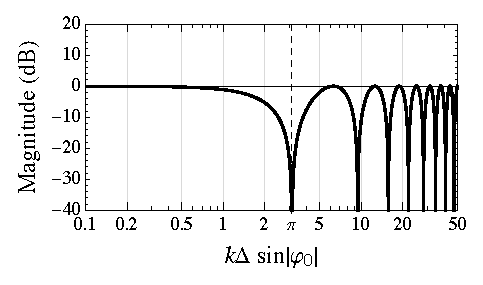
\includegraphics[width = 0.49\textwidth]{08_proposed_method/figures/nonDimFreqResp_xf.eps}
  \caption{Comb-filter magnitude responses caused by the weighted average method.}
  \label{fig:08_Proposed_Method:XF_CombFiltering_NonDim}
\end{figure} %%NOTE%% vertical axis label is too complicated: |A0 / B0ref| or something

Similarly, in \figref{fig:08_Proposed_Method:XF_CombFiltering}, we plot the same magnitude responses of $A_0$ but for a fixed microphone spacing of $\Delta = 0.5$~m and for particular source azimuths.
Note that due to the lateral symmetry of the geometry, these responses hold for negative azimuths ($\varphi_0' = -\varphi_0$),
and due to the front-back symmetry, they also hold for rear azimuths ($\varphi_0' = 180^\circ \pm \varphi_0$).
From this plot, we see that only sources at $0^\circ$ (or $180^\circ$) azimuth are interpolated without comb-filtering.
For all other azimuths, comb-filtering is introduced due to the time-of-arrival delay between microphones.

\begin{figure}[t]
\centering
  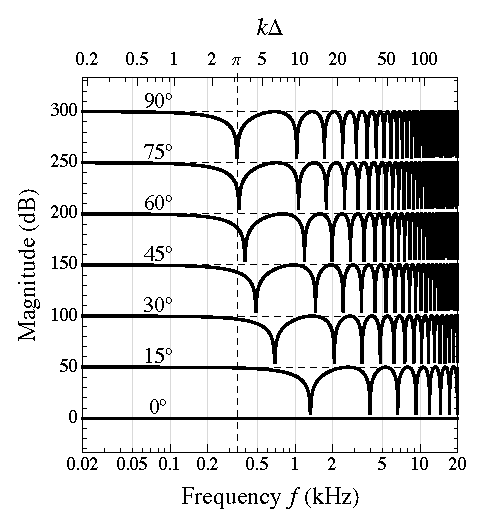
\includegraphics[width = 0.49\textwidth]{08_proposed_method/figures/freqResp_xf.eps}
  \caption[Comb-filter magnitude responses caused by the weighted average method.]{
  Comb-filter magnitude responses caused by the weighted average method for various source azimuths.
  The bottom axis shows frequency in kHz for a microphone spacing of $\Delta = 0.5$~m while the top axis shows the nondimensional frequency $k\Delta$.
  For legibility, each frequency response is offset by $50$~dB and notch depths have been artificially truncated to not exceed $-45$~dB.}
  \label{fig:08_Proposed_Method:XF_CombFiltering}
\end{figure} %%NOTE%% vertical axis label is too complicated: |A0 / B0ref| or something

%%%% Precedence-effect errors %%%%
\subsection{Localization: precedence-effect errors}
For a plane-wave source, the localization information received by each microphone will be identical, so localization of the interpolated signal is likely unchanged.
However, for a finite-distance source, the apparent source direction will differ between the perspectives of each microphone.
In such cases, interpolation between the microphones effectively leads to the creation of distinct \textit{virtual sources}, as illustrated in~\figref{fig:08_Proposed_Method:Effective_Sources}.

% Diagram of effective source positions
\begin{figure}[t]
\centering
  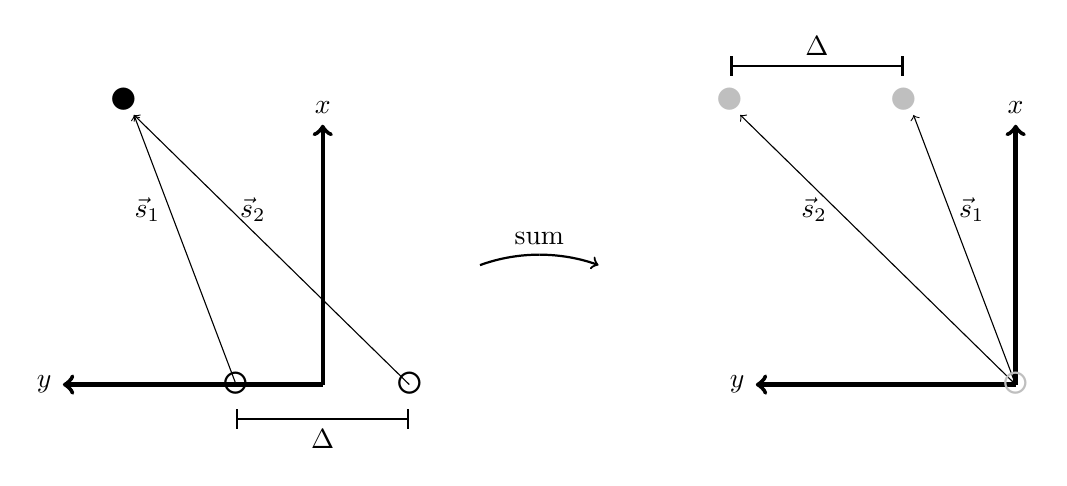
\begin{tikzpicture}[scale=2.2]
% Parameters
\def\radius{1.5};
\def\arrowScale{0.95};
\def\plotOffset{2}

\def\micSpacing{1};
\def\micL{-0.5*\micSpacing};
\def\micR{0.5*\micSpacing};

\def\sourceRadius{2};
\def\sourceAzimuth{35}
\pgfmathsetmacro\sourceY{cos(-\sourceAzimuth)*\sourceRadius}
\pgfmathsetmacro\sourceX{sin(-\sourceAzimuth)*\sourceRadius}

\pgfmathsetmacro\sourceLAzimuth{-atan((\sourceX-\micL)/\sourceY)}
\pgfmathsetmacro\sourceRAzimuth{-atan((\sourceX-\micR)/\sourceY)}

% Coordinate system
\draw[ultra thick,->] (0-\plotOffset,0) -- (0-\plotOffset,\radius) node[above]{$x$};
\draw[ultra thick,->] (0-\plotOffset,0) -- (-\radius-\plotOffset,0) node[left]{$y$};

% Source
\node at (\sourceX-\plotOffset,\sourceY){\huge $\bullet$}; % source
\draw[->] (\micL-\plotOffset,0) -- (\arrowScale*\sourceX-\plotOffset,\arrowScale*\sourceY) node[left, pos=0.65]{$\vec{s}_1$}; % left mic
\draw[->] (\micR-\plotOffset,0) -- (\arrowScale*\sourceX-\plotOffset,\arrowScale*\sourceY) node[right, pos=0.65]{$\vec{s}_2$}; % right mic

% Mic positions
\node at (\micL-\plotOffset,0){\huge $\circ$};
\node at (\micR-\plotOffset,0){\huge $\circ$};
\draw[thick,|-|] (\micL-\plotOffset,-0.2) -- (\micR-\plotOffset,-0.2) node[below, pos=0.5]{$\Delta$};

% Transformation
\draw[thick,-] (0-\radius/2,\radius/2) arc(90:110:1cm); \draw[thick,->] (0-\radius/2,\radius/2) node[above]{sum} arc(90:70:1cm);

% Effective coordinate system
\draw[ultra thick,->] (0+\plotOffset,0) -- (0+\plotOffset,\radius) node[above]{$x$};
\draw[ultra thick,->] (0+\plotOffset,0) -- (-\radius+\plotOffset,0) node[left]{$y$};

% Effective sources
\node at (\sourceX+\plotOffset+\micL,\sourceY){\huge $\color{lightgray}{\bullet}$}; % left source
\node at (\sourceX+\plotOffset+\micR,\sourceY){\huge $\color{lightgray}{\bullet}$}; % right source
\draw[->] (0+\plotOffset,0) -- (\arrowScale*\sourceX+\plotOffset-\micL,\arrowScale*\sourceY) node[right, pos=0.65]{$\vec{s}_1$}; % left mic
\draw[->] (0+\plotOffset,0) -- (\arrowScale*\sourceX+\plotOffset-\micR,\arrowScale*\sourceY) node[left, pos=0.65]{$\vec{s}_2$}; % right mic

% Effective mic position
\node at (0+\plotOffset,0){\huge $\color{lightgray}{\circ}$};
\draw[thick,|-|] (\micL+\plotOffset+\sourceX,\sourceY+0.2) -- (\micR+\plotOffset+\sourceX,\sourceY+0.2) node[above, pos=0.5]{$\Delta$};

\end{tikzpicture}
  \caption[Diagram of virtual sources created by the weighted average method.]{
  Diagram of virtual sources (light gray filled circles) effectively created by the weighted average method for a pair of microphones (empty circles) in a sound field with a single source (black filled circle).}
  \label{fig:08_Proposed_Method:Effective_Sources}
\end{figure}

To explore the potential localization errors created by these virtual sources, we employ the precedence-effect-based localization model of \citet{Stitt2016}, as described here in \secref{sec:04_Auditory_Models:PE_Energy_Vector}.
This model takes as inputs the source positions (in this case, $\vec{s}_1$ and $\vec{s}_2$) and signal amplitudes (the interpolation weights $w_1$ and $w_2$ from \eqnref{eq:03_Navigation_Techniques:Crossfading}), and computes a predicted localization vector, $\vec{\nu}_\text{PE}$.
Here we let the free parameter, $\alpha$, as defined by~\citeauthor{Stitt2016}, take a value of $\alpha = 0.6$, which is somewhat typical for a stimulus signal consisting of both transient and stationary components \citep{Stitt2016}.
We then compute, using the real source position ($\vec{s}_0$) and the desired listener position ($\vec{r}_0$), a localization error, $e_\nu$, given by \eqnref{eq:04_Auditory_Models:Localization_Error} with $\vec{\nu}$ replaced by $\vec{\nu}_\text{PE}$ (and with $\vec{s}_0{}' = \vec{s}_0 - \vec{r}_0$).
%\begin{equation}\label{eq:08_Proposed_Method:Localization_Error}
%e_\nu = \cos^{-1} \left( \hat{\nu}_\text{PE} \cdot \frac{\vec{s}_0 - \vec{r}_0}{\|\vec{s}_0 - \vec{r}_0\|} \right),
%\end{equation}
%where $\|\cdot\|$ denotes the $\ell^2$ norm (Euclidean distance) of a vector.

In \figref{fig:08_Proposed_Method:XF_PrecedenceErrors}, we plot these predicted localization errors, averaged over the entire navigable region (as defined in \secref{sec:06_Simulation_Framework:Linear_Geometry}) and all source azimuths, for various combinations of source distance $s_0$ and microphone spacing $\Delta$.
%In this simulation, we vary the source azimuth from $\varphi_0 = 0^\circ$ to $90^\circ$ in increments of $5^\circ$, and the listener position from $y_0 = -\Delta/2$ to $\Delta/2$ in 30 equal increments.
Note that we exclude from this contour plot the region in which $s_0 + \Delta / 2 < 0.1$~m
(i.e., the bottom left corner of \figref{fig:08_Proposed_Method:XF_PrecedenceErrors}), as this corresponds to geometries for which the source is
``inside the head'' (for an approximate head radius of 10~cm) at all positions within the navigable region.

\begin{figure}[t]
\centering
  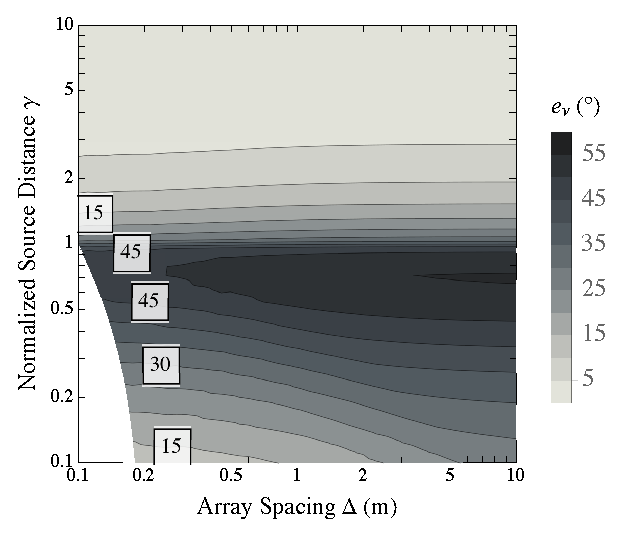
\includegraphics[width = 0.49\textwidth]{08_proposed_method/figures/stitt2016_a60_contour_xf.eps}
  \caption[Localization contour plot for the weighted average method.]{
  Predicted localization errors $e_\nu$ incurred by the weighted average method
  for various combinations of microphone spacing $\Delta$ and normalized source distance $\gamma = s_0 / (\Delta / 2)$.
  The plotted errors have been averaged over the entire navigable region (as defined in~\secref{sec:06_Simulation_Framework:Linear_Geometry})
  and all source azimuths ($\varphi_0 \in [0,90^\circ]$ in increments of $5^\circ$).
  Contour lines are drawn every $5^\circ$.}
  \label{fig:08_Proposed_Method:XF_PrecedenceErrors}
\end{figure}

From this plot, we first note that localization errors appear primarily dependent on $\gamma$, but tend to increase with increasing $\Delta$.
We also see that, at large microphone spacings ($\Delta > 0.5$~m), localization errors for ``slightly'' interior sources ($0.5 < \gamma < 1$) become extreme ($e_\nu > 50^\circ$).
Localization errors for distant exterior sources ($\gamma > 2$), however, are uniformly small ($e_\nu < 10^\circ$).
Although not shown here, it can be verified that these localization errors tend to decrease with increasing $\alpha \in [0,1]$,
as $\alpha = 1$ corresponds to purely energy-based localization, with no effect from time-of-arrival delays \citep{Stitt2016}.
Consequently, as $\alpha \to 1$, the dependence of $e_\nu$ on $\Delta$ disappears.

\section{Proposed navigational method}\label{sec:08_Proposed_Method:Proposed_Techniques}
In this section, we first describe our proposed parametric navigational method, which comprises two components:
\begin{enumerate}
\item a parametric method for performing interpolation using only a subset of the microphones, where this subset is determined based on estimated source positions (as described in \secref{sec:08_Proposed_Method:Microphone_Validity}), and
%\item a parametric method for excluding microphones from the interpolation calculation based on estimated source positions (described in \secref{sec:08_Proposed_Method:Microphone_Validity}), and
\item a particular two-band implementation of the regularized least-squares interpolation filters (detailed here in \secreftwo{sec:08_Proposed_Method:Reg-LS_Technique}{sec:08_Proposed_Method:Hybrid_Technique}).
\end{enumerate}
Later in this section, we illustrate basic spectral properties of the interpolation filters in \secref{sec:08_Proposed_Method:Azimuth_Dependence} and briefly discuss practical implementation issues in \secref{sec:08_Proposed_Method:Practical_Implementation}.

%%%% Microphone Validity %%%%
\subsection{Source localization and microphone validity}\label{sec:08_Proposed_Method:Microphone_Validity}
As discussed previously, the ambisonics signals provide a valid description of the captured sound field only in a spherical region around the ambisonics microphone that extends up to the nearest source or obstacle.
Consequently, in order to determine the set of microphones for which the listening position is valid, we must first locate any near-field sources.
Several existing methods for acoustically localizing near-field sources using ambisonics signals from one or more ambisonics microphones are discussed by~\citet[chapter 3]{Zheng2013PhD}, and require only knowledge of the positions and orientations of the microphones.%\footnote{Note that in the present method, we only aim to determine the locations of sources, whereas \citet{Zheng2013PhD} additionally attempts to isolate their emitted signals.}

Briefly, such methods often involve taking a short-time Fourier transform of the first-order ambisonics signals and, for each time-frequency bin, calculating the acoustic intensity vector, as given in \eqnref{eq:04_Auditory_Models:Intensity_Vector}. % \citet[Eq.~(11)]{MerimaaPulkki2005}.
For each ambisonics microphone, a histogram is generated using the direction of the intensity vector at each time and frequency.
The peaks of the histogram indicate source directions, and source positions are determined through triangulation with multiple ambisonics microphones.

Once the locations of the near-field sources are determined, we compare the distances from each microphone to its nearest source and the distance of that microphone to the desired listening position.
Only the signals from those microphones that are nearer to the listening position than to any near-field source are included in the navigation calculation (i.e., all microphones such that $r_p = \|\vec{r}_0 - \vec{u}_p\| < \|\vec{s}_0 - \vec{u}_p\| = s_p$).
A matrix of interpolation filters, described in the following sections, is then computed for and applied to the signals from the remaining ``valid'' microphones.
This procedure is illustrated by the flowchart in \figref{fig:08_Proposed_Method:Flowchart}.

% Flowchart
\begin{figure*}[t]
    \centering
    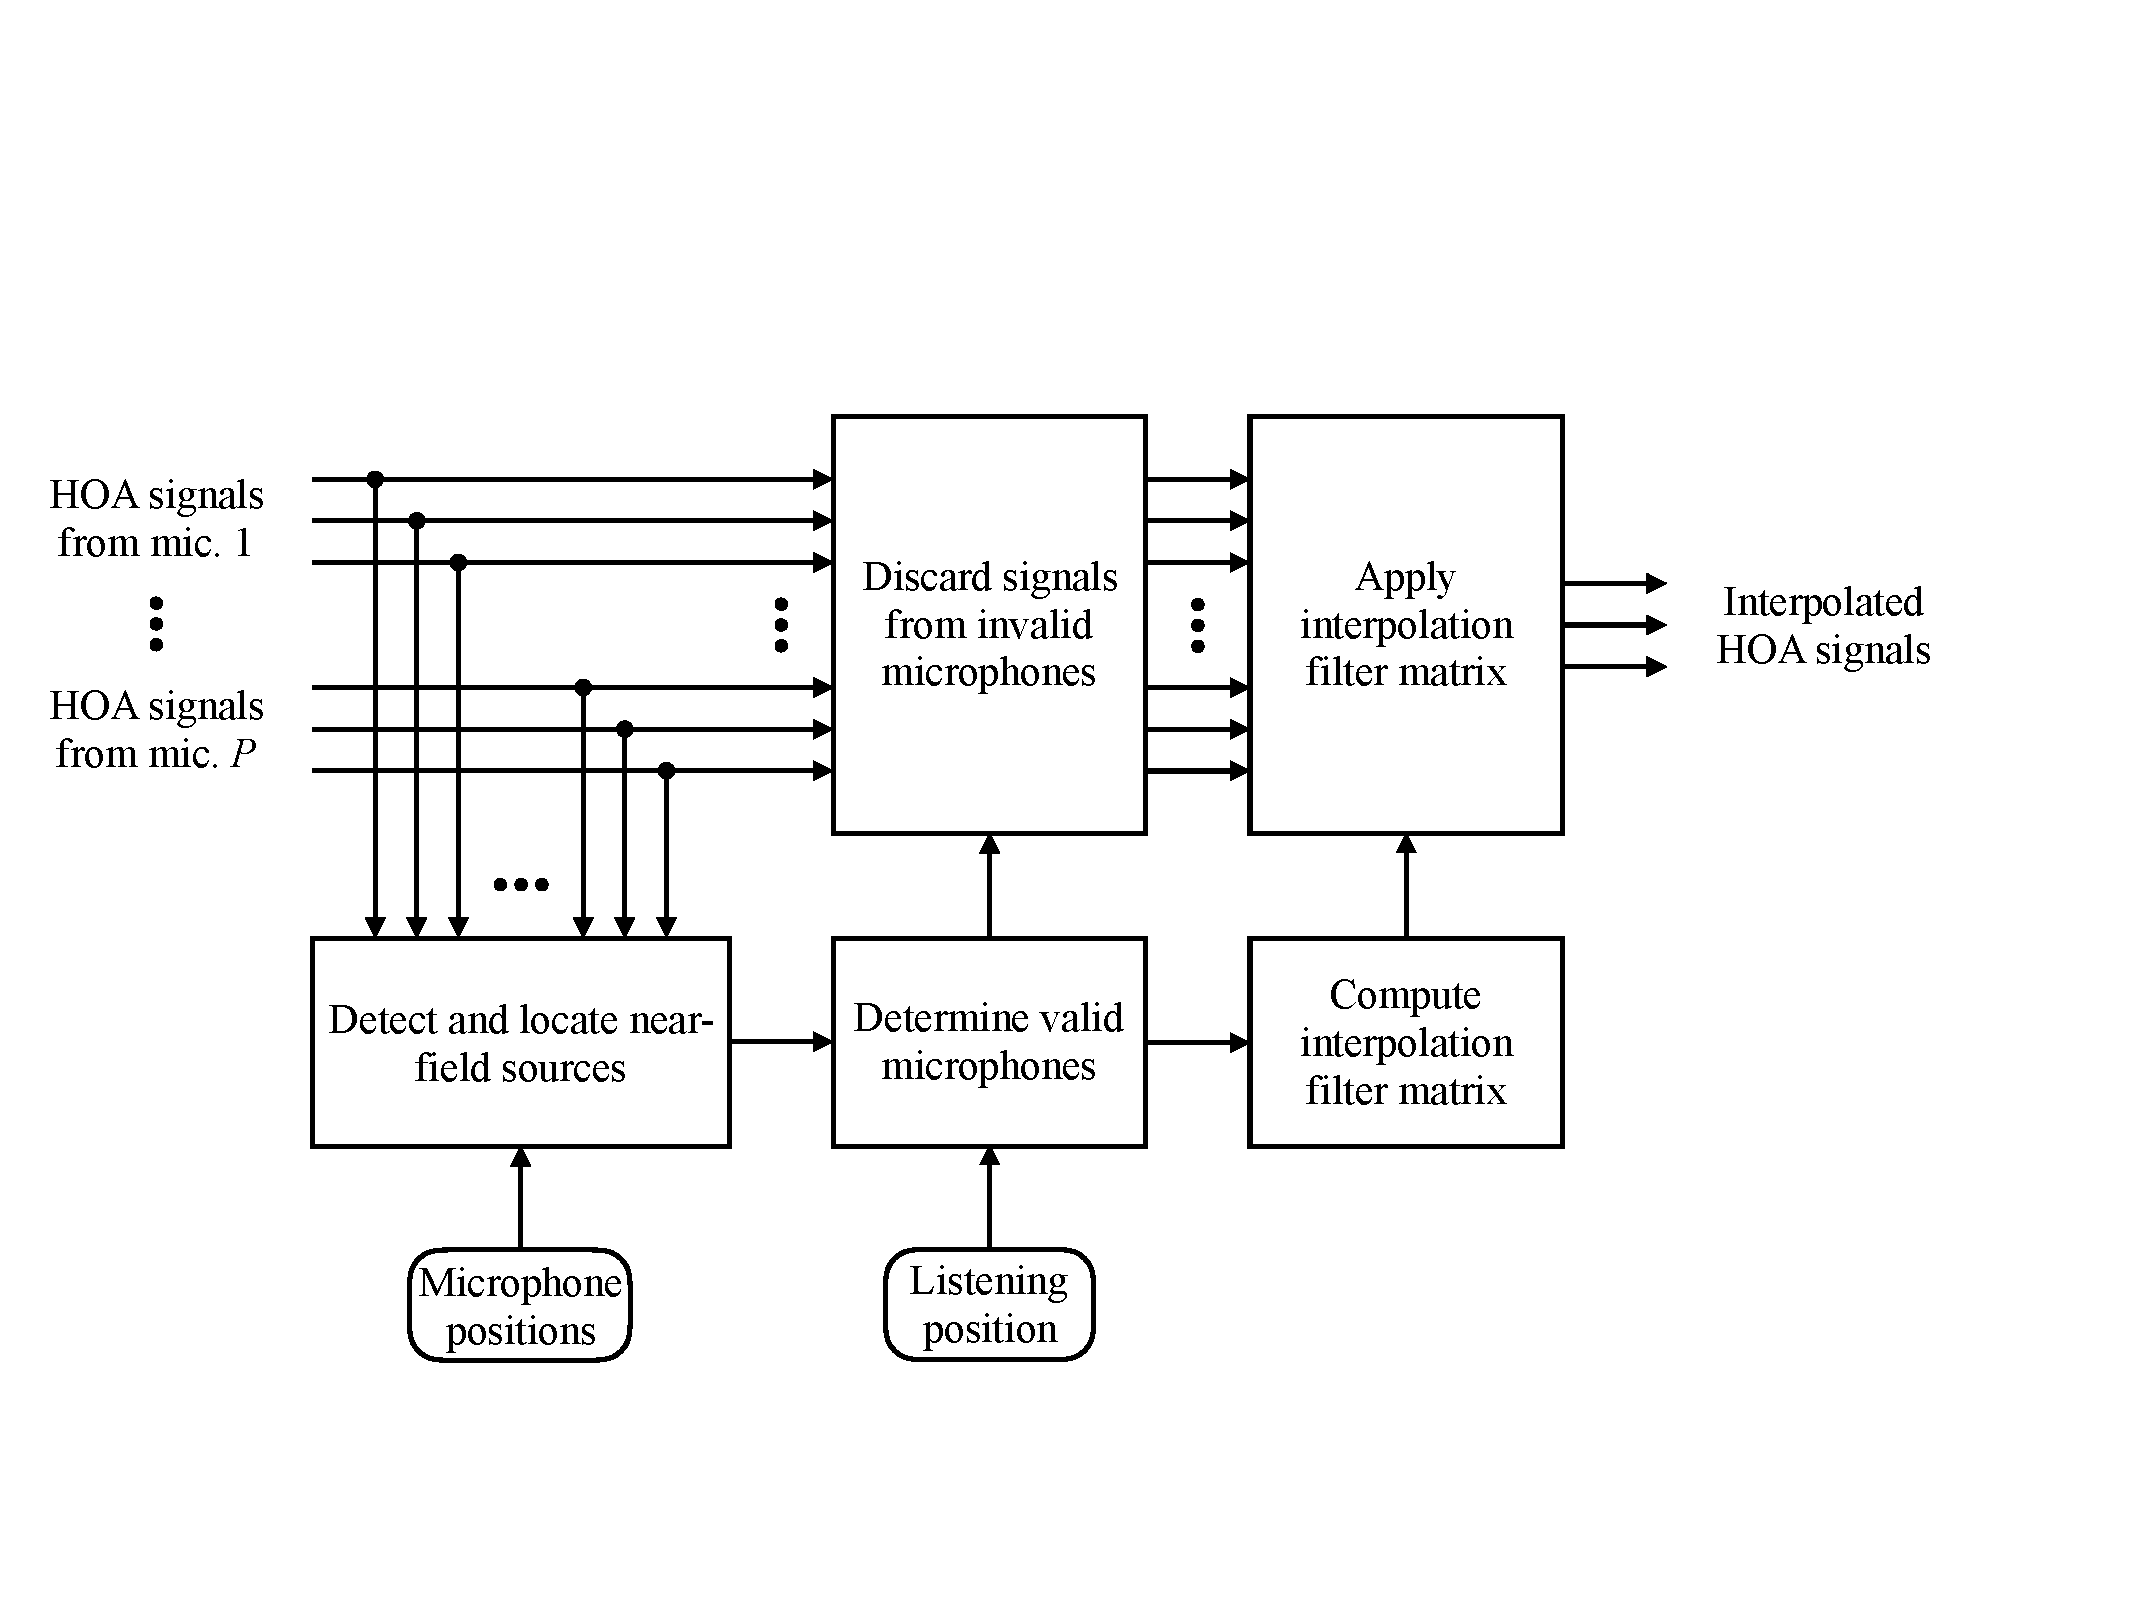
\includegraphics[width = \textwidth,trim={0 4cm 3cm 7cm},clip]{08_proposed_method/figures/Interpolation_Flowchart.pdf}
\caption[Flowchart of the proposed parametric interpolation method.]{
Flowchart of the proposed method for virtual sound field navigation excluding invalid microphones.}
\label{fig:08_Proposed_Method:Flowchart}
\end{figure*}
%%NOTE%% convert to tikz

In this work, we assume that any near-field sound sources can be located accurately and we choose to focus on characterizing the performance of the proposed navigational method under that assumption.
Accordingly, we do not concern ourselves with the sensitivity of the proposed method to inaccuracies in the estimated positions of near-field sources.
This assumption will be valid in scenarios where the positions of the nearest sound sources are either known \textit{a priori} or can be accurately obtained (e.g., through physical distance measurements) \textit{a posteriori}.

%%%% Least-Squares Interpolation Filters %%%%
\subsection{Regularized least-squares interpolation filters}\label{sec:08_Proposed_Method:Reg-LS_Technique}
To compute the interpolation filters, we modify the pseudoinverse-based interpolation method described in \secref{sec:03_Navigation_Techniques:Pinv_Technique} and propose a particular regularization function.
First, we modify \eqnref{eq:03_Navigation_Techniques:Linear_System_Matrices}, such that the matrices are given by
\begin{equation}\label{eq:08_Proposed_Method:Linear_System_Matrices}
\mathbf{M} = 
    \left[ \begin{array}{c}
    \sqrt{w_1} \left( \mathbf{T}(-\vec{r}_1) \right)^\text{T} \\
    \sqrt{w_2} \left( \mathbf{T}(-\vec{r}_2) \right)^\text{T} \\
    \vdots\\
    \sqrt{w_P} \left( \mathbf{T}(-\vec{r}_P) \right)^\text{T}
    \end{array} \right]
,\quad
\mathbf{y} = 
    \left[ \begin{array}{c}
    \sqrt{w_1} \mathbf{b}_1\\
    \sqrt{w_2} \mathbf{b}_2\\
    \vdots\\
    \sqrt{w_P} \mathbf{b}_P
    \end{array} \right],
\end{equation}
where $w_p$ is the interpolation weight for the $p^\textrm{th}$ microphone and recall that $\vec{r}_p = \vec{r}_0 - \vec{u}_p$ is the position of the listener relative to the $p^\textrm{th}$ microphone.

Next, we compute the singular value decomposition of $\mathbf{M}$, such that $\mathbf{M} = \mathbf{U} \Sigma \mathbf{V}^*$, where $(\cdot)^*$ represents conjugate-transposition.
This allows us to compute a regularized pseudoinverse of $\mathbf{M}$, given by \citep[section 5.1]{Hansen1998}
\begin{equation}
\mathbf{L} = \mathbf{V} \Theta \Sigma^{+} \mathbf{U}^*,
\end{equation}
where $(\cdot)^+$ represents pseudoinversion, and $\Theta$ is a square, diagonal matrix whose elements are given by
\begin{equation}
\Theta_{nn} = \frac{\sigma_n^2}{\sigma_n^2 + \beta},
\end{equation}
where $\sigma_n$ is the $n^\textrm{th}$ singular value of $\mathbf{M}$, with $n \in [1,N_\textrm{max}]$.
(Recall that $N_\textrm{max} = (L_\textrm{max} + 1)^2$ and $L_\textrm{max}$ is defined in \eqnref{eq:03_Navigation_Techniques:Pinv_Interpolation_Lmax}.)
In general, the regularization parameter $\beta$ may be a function of frequency.
Here, we choose the magnitude of a high-shelf filter as the regularization function, given by \citep[section 5.2]{Zolzer2008}
\begin{equation}
\beta(k) = \beta_0 \left| \frac{G_{\pi} i \frac{k}{k_0} + 1}{i \frac{k}{k_0} + G_{\pi}} \right|,
\end{equation}
where $G_{\pi}$ is the amplitude of the high-shelf filter and $k_0$ is its zero-dB crossing, which, for convenience, we take to be the same as that given below in \eqnref{eq:08_Proposed_Method:Hybrid_XO_Freq}.
(In our original publication, we had chosen $k_0 = 1 / \Delta$ for simplicity \citep[Eq.~(17)]{TylkaChoueiri2016}, but we did not consider cases where $P \neq 2$.)
We then let
\begin{equation}
\beta_0 = \frac{1}{\sigma_0} \max_n \sigma_n,
\end{equation}
with some constant $\sigma_0 \gg 1$.
Note that the singular values ($\sigma_n$) of $\mathbf{M}$ are calculated for each frequency, so, in general, $\beta_0$ is also frequency-dependent.
Here, we choose $G_{\pi} = 10^{1.5}$ (i.e., 30~dB) and $\sigma_0 = 1000$.

Finally, we obtain an estimate of $\mathbf{a}$ at each $k$, given by
\begin{equation}
\mathbf{\tilde{a}}(k) = \mathbf{L}(k) \cdot \mathbf{y}(k).
\end{equation}
Note that, as with the weighted average method, we may choose to drop the higher-order terms in $\mathbf{\tilde{a}}$ such that we keep only up to order $L_\textrm{out}$, where $L_\textrm{out} \leq L_\textrm{max}$.

Also note that we can factor out the interpolation weights into a diagonal matrix, such that
\begin{equation}
\mathbf{\tilde{a}}(k) = \left( \mathbf{L}(k) \cdot
    \left[ \begin{array}{c c c c}
    \sqrt{w_1}\, \mathbf{I} & \mathbf{0} & \cdots & \mathbf{0}\\
    \mathbf{0} & \sqrt{w_2}\, \mathbf{I} & \ddots & \vdots\\
    \vdots & \ddots & \ddots & \mathbf{0}\\
    \mathbf{0} & \cdots & \mathbf{0} & \sqrt{w_P}\, \mathbf{I}
    \end{array} \right]
 \right) \cdot
     \left[ \begin{array}{c}
    \mathbf{b}_1(k)\\
    \mathbf{b}_2(k)\\
    \vdots\\
    \mathbf{b}_P(k)
    \end{array} \right],
\end{equation}
where $\mathbf{0}$ is an $N_\textrm{in} \times N_\textrm{in}$ matrix of zeros, and $\mathbf{I}$ is the $N_\textrm{in} \times N_\textrm{in}$ identity matrix.
For compactness, we let
\begin{equation}
\mathbf{L}_w(k) = \mathbf{L}(k) \cdot
    \left[ \begin{array}{c c c c}
    \sqrt{w_1}\, \mathbf{I} & \mathbf{0} & \cdots & \mathbf{0}\\
    \mathbf{0} & \sqrt{w_2}\, \mathbf{I} & \ddots & \vdots\\
    \vdots & \ddots & \ddots & \mathbf{0}\\
    \mathbf{0} & \cdots & \mathbf{0} & \sqrt{w_P}\, \mathbf{I}
    \end{array} \right].
\end{equation}

%%%% Hybrid Filters %%%%
\subsection{Two-band interpolation filters}\label{sec:08_Proposed_Method:Hybrid_Technique}
As found in a previous analysis, the regularized least-squares interpolation filters derived in the previous section can induce significant spectral coloration at high frequencies, whereas, below some critical frequency, they induce negligible coloration \citep[cf.~Fig.~4b]{TylkaChoueiri2016}.
%In particular, in the case of $P = 2$ microphones, this critical frequency was found to correspond to $k \Delta \approx 2 L_\textrm{in}$ \citep[cf.~Fig.~5]{TylkaChoueiri2016}.
Consequently, we propose a two-band approach which applies the regularized least-squares interpolation filters at low frequencies ($k < k_0$) and employs the weighted average method at higher frequencies ($k \geq k_0$).
Here, we let
\begin{equation}\label{eq:08_Proposed_Method:Hybrid_XO_Freq}
k_0 = \left\{
  \begin{array}{c l}
  \displaystyle \frac{1}{r_1}, & \text{for } P = 1,\\[8pt]
  \displaystyle \frac{\Delta}{r_1 r_2}, & \text{for } P = 2,\\[8pt]
  \displaystyle \frac{1}{\max_{p\in[1,P]} r_p}, & \text{otherwise},
  \end{array} \right.
\end{equation}
which we found empirically to perform well in terms of coloration.

We then rewrite the weighted average calculation, given in \eqnref{eq:03_Navigation_Techniques:Crossfading}, as a matrix equation, such that
\begin{equation}
\mathbf{\tilde{a}}(k) = 
    \left[ \begin{array}{c c c c}
    w_1 \mathbf{I} & w_2 \mathbf{I} & \cdots & w_P \mathbf{I}
    \end{array} \right]
\cdot
     \left[ \begin{array}{c}
    \mathbf{b}_1(k)\\
    \mathbf{b}_2(k)\\
    \vdots\\
    \mathbf{b}_P(k)
    \end{array} \right],
\end{equation}
where now $\mathbf{I}$ is the $N_\textrm{out} \times N_\textrm{in}$ identity matrix. %%NOTE%% num rows could be N_in, N_max, or N_out
Thus, we define the combined interpolation filter matrix as
\begin{equation}\label{eq:08_Proposed_Method:HybridFilters}
\mathbf{H}(k) = \left\{
  \begin{array}{c l}
  \mathbf{L}_w(k), & \textrm{for } k < k_0, \\
  \left[
    \begin{array}{c c c c}
    w_1 \mathbf{I} & w_2 \mathbf{I} & \cdots & w_P \mathbf{I}
    \end{array}
  \right], & \textrm{for } k \geq k_0.
  \end{array} \right.
\end{equation}
Note that if we have only $P = 1$ valid microphone, the high-frequency filter matrix becomes the identity matrix (since $w_1 = 1$ after normalization).

Given the well-established rule of thumb that a sound field is accurately represented up to a distance $r$ provided that $k r \leq L_\textrm{in}$ \citep{WardAbhayapala2001}, we expect that for $P = 1$, the coloration should be negligible below $k r_1 \approx L_\textrm{in}$.
Additionally, for $P = 2$ microphones, we previously found that coloration appeared negligible below $k \Delta \approx 2 L_\textrm{in}$ for a listener equidistant from the microphones \citep[cf.~Fig.~5]{TylkaChoueiri2016}.
However, these approximations were found to break down due to the near-field compensation filters needed in practice (described in \secref{sec:02_Acoustical_Theory:Ambisonics_Encoding}).
Consequently, here we take a more conservative critical frequency, as in \eqnref{eq:08_Proposed_Method:Hybrid_XO_Freq}.%
\footnote{Note that in this work we do not explore the case of $P > 2$, so a superior critical frequency likely exists.
It may also still be worth pursuing order-dependent critical frequencies for $P = 1,2$, since, in principle, increasing the expansion order should improve accuracy, but we do not do so here.}

%%%% Source Azimuth Dependence %%%%
\subsection{Source azimuth dependence}\label{sec:08_Proposed_Method:Azimuth_Dependence}
In this section, we examine the effective frequency responses induced by translation via the regularized least-squares and hybrid interpolation filters as a function of source azimuth.
As described in \secref{sec:06_Simulation_Framework:Azimuth_Dependence}, for these simulations, we let $L_\text{in} = 4$, pick $\Delta = 0.5$~m and $s_0 = 2.5$~m (so $\gamma = 10$), and interpolate to $\vec{r}_0 = (0, 0, 0)$.
(Recall that these quantities are defined in \secref{sec:06_Simulation_Framework:Linear_Geometry} for a linear array geometry.)

The induced frequency responses are plotted in \figref{fig:08_Proposed_Method:Azimuth_Dependence}.
For the regularized least-squares interpolation filters (see \figref{fig:08_Proposed_Method:Azimuth_Dependence:Pinv}), we see that the frequency response is largely flat below a critical frequency (cf.~\citet[Fig.~4b]{TylkaChoueiri2016}), whereas above that frequency, the response exhibits significant broadband deviations (e.g., for $\varphi_0 = 75^\circ, 90^\circ$) as well as sporadic notches.
Based on well-established psychoacoustic findings, we can expect these distortions to be more audible (that is, either more likely to be audible or more significantly distorted) than the comb-filtering response of the weighted average method \citep{Bucklein1981,Kates1984,Brunner2007}.%
\footnote{In particular, \citet{Bucklein1981} showed that spectral peaks are more audible than notches of the same width and height, and that broadband spectral features are more audible than narrow ones.
Additionally, psychoacoustic studies have shown that comb-filter responses can be imperceptible if the time-delay between the primary and secondary signals is long enough and/or if their relative levels are different enough \citep{Kates1984,Brunner2007}.}

\begin{figure*}[t]
    	\centering
    	\begin{subfigure}[b]{0.49\textwidth}
        		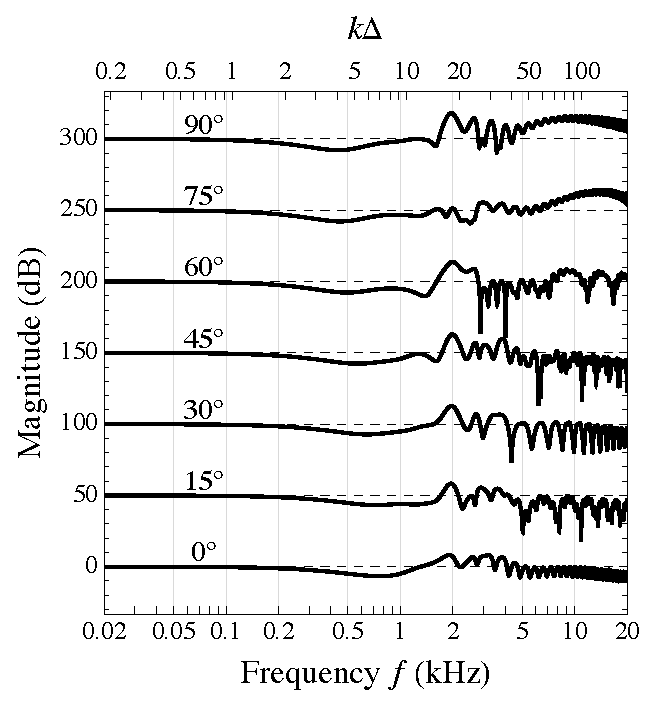
\includegraphics[width=\textwidth]{08_proposed_method/figures/sourceAz_freqResp_pinv.eps}
        		\caption{Regularized least-squares filters}
        		\label{fig:08_Proposed_Method:Azimuth_Dependence:Pinv}
    	\end{subfigure}
	\hfill
    	\begin{subfigure}[b]{0.49\textwidth}
        		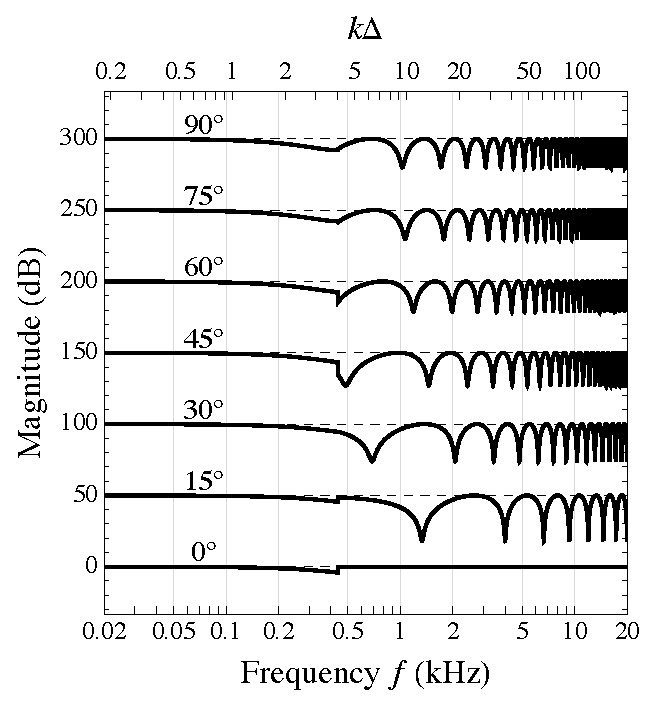
\includegraphics[width=\textwidth]{08_proposed_method/figures/sourceAz_freqResp_validhybrid.eps}
        		\caption{Hybrid filters}
        		\label{fig:08_Proposed_Method:Azimuth_Dependence:Hybrid}
    	\end{subfigure}
	
	\caption[Magnitude responses across azimuths for each interpolation filter.]{
	Magnitude responses caused by the regularized least-squares and hybrid interpolation filters for various source azimuths.
  The bottom axes show frequency in kHz while the top axes show the nondimensional frequency $k\Delta$ for a microphone spacing of $\Delta = 0.5$~m.
  For legibility, each frequency response is offset by $50$~dB and the responses have been artificially truncated (where needed) to not exceed $-45$~dB.}
	\label{fig:08_Proposed_Method:Azimuth_Dependence}
\end{figure*} %%NOTE%% vertical axis label is too complicated: |A0 / B0ref| or something

As shown in \figref{fig:08_Proposed_Method:Azimuth_Dependence:Hybrid}, the hybrid filters exhibit precisely this comb-filtering frequency response above the critical frequency, $k_0$, given in \eqnref{eq:08_Proposed_Method:Hybrid_XO_Freq}.
Below this critical frequency, however, the hybrid filter responses exhibit a wide, flat region, rather than the continued comb-filtering response exhibited by the weighted average method (as shown in \figref{fig:08_Proposed_Method:XF_CombFiltering}).
Consequently, we expect the coloration incurred by the hybrid filters to be less severe than that incurred by the weighted average method.

%%%% Practical Implementation %%%%
\subsection{Practical implementation}\label{sec:08_Proposed_Method:Practical_Implementation}
In practice, as the listener traverses the navigable region, the number of valid microphones may change.
Consequently, one should crossfade between audio frames to prevent any audible discontinuities caused by a sudden change in the filters.
Additionally, it is likely preferable to implement a ``crossover'' between the low- and high-frequency ranges of the combined filter matrix, thereby blending the two filter matrices.
Here, however, we take a simple frequency-domain concatenation approach, as indicated in \eqnref{eq:08_Proposed_Method:HybridFilters}.

%If $\mathbf{M}$ is singular, such that $\mathbf{M}^+$ is undefined, we ``dither'' the weights $w_p$.

Although in this work we only consider interpolation to points within the strictly-interior navigable region (i.e., the area spanned by the microphone array), navigation outside of this region may be achieved in practice through a two-stage navigation approach.
In such an approach, the recorded signals are first interpolated to the point within the strictly-interior region nearest to the desired listening position.
Then, those interpolated signals are effectively treated as a new virtual ambisonics microphone and extrapolated to the desired listening position.

\section{Characterization and discussion}\label{sec:08_Proposed_Method:Results}
% Level

Level errors (as defined in \secref{sec:04_Auditory_Models:Audible_Energy}) for each method are shown in \figref{fig:08_Proposed_Method:Level_Errors}.
From these plots, we see that both methods exhibit similar behavior in that the reproduced level of an interior source ($\gamma < 1$) is several dB too low and decreases with decreasing $\gamma$.
For the weighted average method, we can understand this behavior by considering that, for an interior source, the navigable region consists primarily of positions at which the source is closer to the listener than it is to either microphone.
(That is, $\|\vec{s}_0 - \vec{r}_0\| < \|\vec{s}_0 - \vec{u}_p\|$ for both $p = 1, 2$.)
Consequently, the reproduced level should be increased beyond that recorded by either microphone.
However, by construction (recall \secref{sec:03_Navigation_Techniques:XF_Technique}), the weighted average method can only produce levels that are at most equal to that recorded by the microphone that is nearer to the source.
Therefore, it is unsurprising that the weighted average method cannot adequately reproduce the signal levels of interior sources.

\begin{figure*}[t]
    	\centering
    	\begin{subfigure}[b]{0.49\textwidth}
        		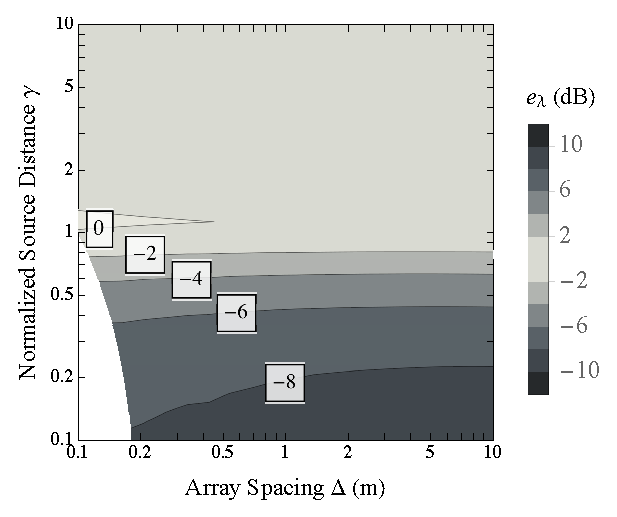
\includegraphics[width=\textwidth]{08_proposed_method/figures/audibleEnergy_contour_xf.eps}
        		\caption{Weighted average method}
        		\label{fig:08_Proposed_Method:Level_Errors:XF}
    	\end{subfigure}
	\hfill
	\begin{subfigure}[b]{0.49\textwidth}
        		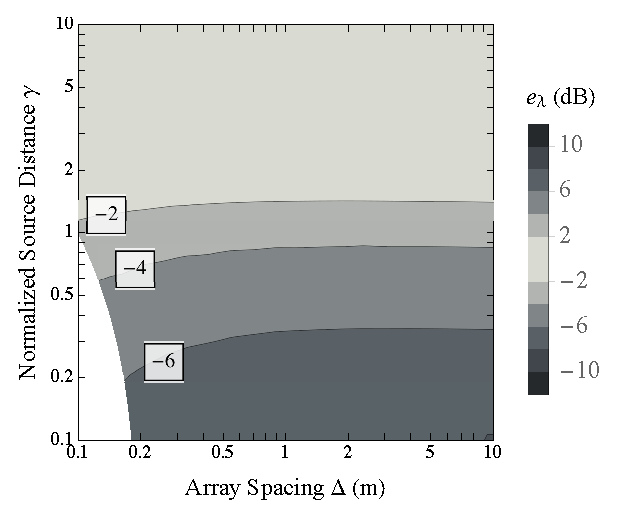
\includegraphics[width=\textwidth]{08_proposed_method/figures/audibleEnergy_contour_validhybrid.eps}
        		\caption{Proposed method}
        		\label{fig:08_Proposed_Method:Level_Errors:Hybrid}
    	\end{subfigure}
	
    	\caption[Contour plots of level errors for each interpolation method.]{
	Level errors $e_\lambda$ for microphone spacing $\Delta$ and normalized source distance $\gamma$.
  Contour lines are drawn every $2$~dB.}
    	\label{fig:08_Proposed_Method:Level_Errors}
\end{figure*}

For the proposed method, a similar problem is encountered.
Note that, for interior sources, typically only one microphone will be valid for any given listening position, and, in such cases, the signals from that microphone are used ``as is'' for the upper portion of the frequency range (see \eqnref{eq:08_Proposed_Method:HybridFilters}).
However, as discussed above, for those listening positions, the amplitude of the signals should increase, since the source will be closer to the listener than it is to the microphone. %%NOTE%% prove this?
So again, it is unsurprising that the proposed method does not achieve a sufficient reproduced level for interior sources.

These errors may be particularly detrimental to a listener's perception of source distance as the listener navigates closer to a source since one of the primary distance cues humans expect is an increase in level \citep[section 3.1.1]{Zahorik2005}.
Consequently, the impact of these errors on a listener's perception of distance should be investigated, although it is outside the scope of this work to do so.

From \figref{fig:08_Proposed_Method:Level_Errors:Hybrid}, we note that the proposed method achieves a minor improvement ($\sim2$~dB) over the weighted average method for far interior sources, approximately $\gamma < 0.4$.
This is primarily due to the exclusion of the invalid microphone by the proposed method, which prevents the comb-filtering introduced by the weighted average method which decreases the average level.
However, the proposed method yields a minor degradation compared to the weighted average method for $\gamma \approx 1$.

As the behavior seen in these plots appears consistent and predictable, one might expect that it would be straightforward to correct with a gain factor, especially for the proposed method since an estimate of the source position is already required for the microphone validity calculation.
However, such a correction would not be viable for sound fields consisting of more than a single source, since, the levels of exterior sources are currently reproduced accurately, and any gain correction would corrupt those sources' signals.

% Coloration

Spectral errors (as defined in \secref{sec:04_Auditory_Models:Coloration_Metrics:ABSE}) for each method are shown in \figref{fig:08_Proposed_Method:Spectral_Errors}.
From these plots, we see that, at large spacings ($\Delta > 0.5$~m) with an interior source ($\gamma < 1$), the proposed method achieves significantly ($\sim 4$~dB) smaller spectral errors than the weighted average method.
This too is primarily due to the exclusion of the invalid microphone from the navigation calculation, which prevents any comb-filtering in the proposed method.

\begin{figure*}[t]
    	\centering
    	\begin{subfigure}[b]{0.49\textwidth}
        		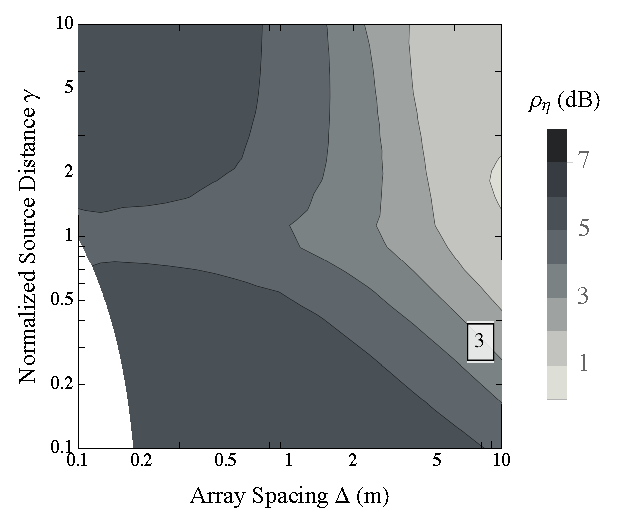
\includegraphics[width=\textwidth]{08_proposed_method/figures/scharer2009_contour_xf.eps}
        		\caption{Weighted average method}
        		\label{fig:08_Proposed_Method:Spectral_Errors:XF}
    	\end{subfigure}
	\hfill
	\begin{subfigure}[b]{0.49\textwidth}
        		\includegraphics[width=\textwidth]{08_proposed_method/figures/scharer2009_contour_validhybrid.eps}
        		\caption{Proposed method}
        		\label{fig:08_Proposed_Method:Spectral_Errors:Hybrid}
    	\end{subfigure}
	
    	\caption[Contour plots of spectral errors for each interpolation method.]{
	Spectral errors $\rho_\eta$ for microphone spacing $\Delta$ and normalized source distance $\gamma$.
  Contour lines are drawn every $1$~dB.}
    	\label{fig:08_Proposed_Method:Spectral_Errors}
\end{figure*}

Additionally, at small microphone spacings ($\Delta < 0.5$~m) with an exterior source ($\gamma > 1$), the proposed method achieves slightly ($\sim 1$~dB) smaller spectral errors than the weighted average method.
This is due to the widening (as $\Delta$ decreases) of the frequency range over which the regularized least-squares interpolation filters achieve a nearly flat frequency response (see \figref{fig:08_Proposed_Method:Azimuth_Dependence}). % (cf.~\citet[Fig.~4b]{TylkaChoueiri2016}).
As specified in \eqnref{eq:08_Proposed_Method:Hybrid_XO_Freq}, for $P = 2$ microphones, the crossover frequency increases with decreasing $\Delta$, since $r_1 r_2 \propto \Delta^2$.
At large microphone spacings ($\Delta > 0.5$~m) with an exterior source ($\gamma > 1$), the proposed and weighted average methods perform comparably.

% Localization

Localization errors (as computed with \eqnref{eq:04_Auditory_Models:Localization_Error} for the localization model described in \secref{sec:05_Proposed_Models:Localization_Model}) for each method are shown in \figref{fig:08_Proposed_Method:Localization_Errors}.
From these plots, we see that, at large spacings ($\Delta > 0.5$~m) with an interior source ($\gamma < 1$), the proposed method achieves significantly (i.e., at least $10^\circ$) smaller localization errors than the weighted average method.
This too is primarily due to the exclusion of the invalid microphone from the navigation calculation, which prevents any corruption of the localization information by the invalid microphone.

\begin{figure*}[t]
    	\centering
    	\begin{subfigure}[b]{0.49\textwidth}
        		\includegraphics[width=\textwidth]{08_proposed_method/figures/tylka2017_contour_xf.eps}
        		\caption{Weighted average method}
        		\label{fig:08_Proposed_Method:Localization_Errors:XF}
    	\end{subfigure}
	\hfill
	\begin{subfigure}[b]{0.49\textwidth}
        		\includegraphics[width=\textwidth]{08_proposed_method/figures/tylka2017_contour_validhybrid.eps}
        		\caption{Proposed method}
        		\label{fig:08_Proposed_Method:Localization_Errors:Hybrid}
    	\end{subfigure}
	
    	\caption[Contour plots of localization errors for each interpolation method.]{
	Predicted localization errors $e_\nu$ for microphone spacing $\Delta$ and normalized source distance $\gamma$.
  Contour lines are drawn every $5^\circ$.}
    	\label{fig:08_Proposed_Method:Localization_Errors}
\end{figure*}

From \figref{fig:08_Proposed_Method:Localization_Errors:Hybrid}, we see that, compared to the weighted average method (see \figref{fig:08_Proposed_Method:Localization_Errors:XF}), the proposed method incurs larger localization errors ($e_\nu > 20^\circ$) for $\Delta < 0.5$~m and $\gamma < 1$ (bottom left corner of the plot).
This penalty may not be too limiting, however, as these values of $\Delta$ and $\gamma$ correspond to sources very near to the origin ($s_0 < 0.25$~m), and in any case, microphone spacings less than $0.5$~m may be impractical.

% Diffuseness

In \figref{fig:08_Proposed_Method:Diffuseness_Errors}, we plot diffuseness errors (as defined in \secref{sec:04_Auditory_Models:Diffuseness_Parameter}) for each method.
For the weighted average method, we see that the diffuseness of the reproduced signals for interior sources ($\gamma < 1$) is too large.
This is due to the increasingly conflicting localization information in the combined signal as $\gamma$ decreases, as illustrated in \figref{fig:08_Proposed_Method:Effective_Sources}.
Consequently, for such interior sources, not only is the localization accuracy degraded, but also the reproduced signals become more diffuse.
For the proposed method, however, the diffuseness is reproduced accurately (i.e., $|e_\Psi| < 0.1$) over almost all conditions, with the exception of at very small $\gamma$ and $\Delta$ (bottom left corner of \figref{fig:08_Proposed_Method:Diffuseness_Errors:Hybrid}).

\begin{figure*}[t]
    	\centering
    	\begin{subfigure}[b]{0.49\textwidth}
        		\includegraphics[width=\textwidth]{08_proposed_method/figures/merimaa2005_d_contour_xf.eps}
        		\caption{Weighted average method}
        		\label{fig:08_Proposed_Method:Diffuseness_Errors:XF}
    	\end{subfigure}
	\hfill
	\begin{subfigure}[b]{0.49\textwidth}
        		\includegraphics[width=\textwidth]{08_proposed_method/figures/merimaa2005_d_contour_validhybrid.eps}
        		\caption{Proposed method}
        		\label{fig:08_Proposed_Method:Diffuseness_Errors:Hybrid}
    	\end{subfigure}
	
    	\caption[Contour plots of diffuseness errors for each interpolation method.]{
	Diffuseness errors $e_\Psi$ for microphone spacing $\Delta$ and normalized source distance $\gamma$.
  Contour lines are drawn in increments of $0.1$.}
    	\label{fig:08_Proposed_Method:Diffuseness_Errors}
\end{figure*}

%% Order Dependence %%
\subsection{Order dependence}\label{sec:08_Proposed_Method:Order_Dependence}
To further explore the performance of these methods, we plot, in \figref{fig:08_Proposed_Method:Order_Errors}, errors in each metric for a source distance of $s_0 = 1$~m and for input ambisonics orders $L_\textrm{in} = 1,2,\dots,6$.
Since $L_\textrm{out} = 1$ in all cases, the weighted average method is only plotted for $L_\textrm{in} = L_\textrm{out} = 1$.

\begin{figure*}[t]
    	\centering
	\begin{subfigure}[b]{0.49\textwidth}
        		\includegraphics[width=\textwidth]{08_proposed_method/figures/audibleEnergy_order.eps}
        		\caption{Level errors $e_\lambda$}
        		\label{fig:08_Proposed_Method:Level_Errors:Order}
    	\end{subfigure}
	\hfill
    	\begin{subfigure}[b]{0.49\textwidth}
        		\includegraphics[width=\textwidth]{08_proposed_method/figures/scharer2009_order.eps}
        		\caption{Spectral errors $\rho_\eta$}
        		\label{fig:08_Proposed_Method:Spectral_Errors:Order}
    	\end{subfigure}
	
	\vspace{0.5cm}
	\begin{subfigure}[b]{0.49\textwidth}
        		\includegraphics[width=\textwidth]{08_proposed_method/figures/tylka2017_order.eps}
        		\caption{Localization errors $e_\nu$}
		\label{fig:08_Proposed_Method:Localization_Errors:Order}
    	\end{subfigure}
	\hfill
    	\begin{subfigure}[b]{0.49\textwidth}
        		\includegraphics[width=\textwidth]{08_proposed_method/figures/merimaa2005_d_order.eps}
        		\caption{Diffuseness errors $e_\Psi$}
		\label{fig:08_Proposed_Method:Diffuseness_Errors:Order}
    	\end{subfigure}
	
    	\caption[Order dependence plots for each interpolation method.]{
	Errors for various microphone spacings $\Delta$ with a fixed source distance $s_0 = 1$~m.
	Errors are plotted for the weighted average method (solid curves) and the proposed method (dashed curves).
	For the proposed method only, six input ambisonics orders are shown: $L_\textrm{in} = 1$ (black) to $L_\textrm{in} = 6$ (lightest gray).}
    	\label{fig:08_Proposed_Method:Order_Errors}
\end{figure*}

From these figures, we immediately see that virtually all errors incurred by the proposed method are identical at all orders.
This result is somewhat surprising, as one might expect higher-order recordings to produce a more accurate interpolated sound field.
Evidently, however, the input ambisonics order does not significantly affect the performance of the proposed method.
This insensitivity to input order is largely due to the order-independent choice of critical frequency, $k_0$, as given in \eqnref{eq:08_Proposed_Method:Hybrid_XO_Freq}.
Potentially, this critical frequency could be optimized to yield improved accuracy as input order increases, at least over a range of array spacings or source positions.
This is a topic for further development.

In \figref{fig:08_Proposed_Method:Spectral_Errors:Order}, we see that, for microphone spacings $0.4 \leq \Delta \leq 1.5$~m, increasing the input order yields increased spectral coloration.
This behavior can be attributed to the mismatch between the near-field compensation filters (given in \eqnref{eq:02_Acoustical_Theory:NearField_HPF}) and the actual low-frequency amplification caused by the near-field effect, as the magnitude of this mismatch increases with order (cf.~\citet[Fig.~6]{Daniel2003b}).
However, at smaller microphone spacings ($\Delta < 0.3$~m), the opposite effect is observed: increasing the order yields a slight improvement in spectral errors.
This is due to the higher-order terms yielding a more accurate estimate of the sound field at the listening position, although this effect is evidently very minor.

In terms of the other three metrics, we see that, for $\Delta < 1$~m, the performance of the proposed method is already nearly optimal (in terms of level, localization, and diffuseness only) with $L_\textrm{in} = 1$.
This implies that the regularized least-squares interpolation filters do not improve the performance of the proposed method by any of these metrics beyond that achieved by the weighted average method; evidently, the dominant effect of these filters is to decrease spectral errors.
For $\Delta > 1$~m, on the other hand, the performance of the proposed method is improved significantly compared to the weighted average method.
This demonstrates that any improvement seen by the proposed method in terms of these metrics (level, localization, or diffuseness) must be primarily due to the exclusion of invalid microphones from the interpolation calculation.

Overall, the results shown in \figref{fig:08_Proposed_Method:Order_Errors} reaffirm our previous finding that the proposed method tends to outperform the weighted average method for interior sources ($\Delta/2 > s_0 = 1$~m).
In \figref{fig:08_Proposed_Method:Level_Errors:Order}, we see that only in a particular range of microphone spacings does the weighted average method outperform the proposed method; beyond approximately $\Delta = 4$~m, the proposed method outperforms the weighted average method.
By all other metrics (\figrefthru{fig:08_Proposed_Method:Spectral_Errors:Order}{fig:08_Proposed_Method:Diffuseness_Errors:Order}), however, the proposed method outperforms the weighted average method at all spacings $\Delta \geq 1$~m.

\section{Conclusions}\label{sec:08_Proposed_Method:Conclusions}
In this chapter, we proposed and characterized an interpolation-based method for virtual navigation, wherein the subset of microphones to be used is parametrically determined to ensure that the region of validity restriction is not violated.
An existing alternative method, in which navigation is performed by computing a weighted average of the ambisonics signals from each microphone, was shown in \secref{sec:08_Proposed_Method:Fundamental_Problems} to incur spectral coloration due to comb-filtering and localization errors due to the precedence effect.
The proposed method, described in \secref{sec:08_Proposed_Method:Proposed_Techniques}, employs knowledge of the locations of any near-field sources in order to determine which ambisonics microphones are valid for use in the navigation calculation as a function of the desired listening position.
Additionally, at low frequencies, the proposed method applies a matrix of regularized least-squares inverse filters to estimate the ambisonics signals at the listening position, while at high frequencies, the weighted average method is employed.

Following the numerical simulation framework laid out in \chapref{chap:06_Simulation_Framework}, we compared the proposed method to the weighted average method.
These two methods were evaluated for a linear array geometry (illustrated in \figref{fig:06_Simulation_Framework:Linear_Geometry}) in terms of the metrics enumerated in \secref{sec:06_Simulation_Framework:Metrics} for sound level, spectral coloration, source localization, and diffuseness.
Results show that, for interior sources (as defined in \figref{fig:06_Simulation_Framework:Linear_Geometry}), both methods fail to achieve a sufficient reproduced sound level.
As sound level is well-known to be a primary distance cue \citep[section 3.1.1]{Zahorik2005}, the impact of these errors on distance perception should be investigated through subjective listening tests.

Otherwise, for interior sources, the proposed method achieves a significant improvement (in terms of coloration, localization, and diffuseness) over the existing method.
In particular, the proposed method yields significantly improved localization errors over the existing method for large microphone spacings (larger than $0.5$~m).
This improvement is primarily a result of excluding the invalid microphone, which would otherwise add spectral coloration, corrupt the localization information, and increase diffuseness in the reproduced signals.
Additionally, for small microphone spacings (smaller than $0.5$~m) and exterior sources, the proposed method achieves slightly smaller spectral errors than does the existing method.
This is due to the widening (as microphone spacing decreases) of the frequency range over which the regularized least-squares interpolation filters achieve a nearly flat frequency response (see \figref{fig:08_Proposed_Method:Azimuth_Dependence}). % (cf.~\citet[Fig.~4b]{TylkaChoueiri2016}).
% this is basically the main result of the sourceAz section

Results also show that the performance of the proposed method is largely independent of the input ambisonics order (see \secref{sec:08_Proposed_Method:Results}).
As this is primarily a consequence of our order-independent choice of critical frequency for the hybrid interpolation filters (see \eqnref{eq:08_Proposed_Method:Hybrid_XO_Freq}), future refinements to the proposed method should explore the use of order-dependent critical frequencies in an effort to better leverage the additional information about the sound field contained in the higher-order signals.
Ideally, this information could be used to further improve localization accuracy for interior sources and/or mitigate the spectral coloration induced by the proposed method for exterior sources.

The results presented in this chapter further corroborate the primary finding of \chapref{chap:07_Characterization_Extrapolation}: that violating the region of validity restriction introduces significant errors (in this case, primarily in terms of coloration and localization).
As demonstrated here, our proposed method successfully mitigates these errors by parametrically ensuring that the region of validity restriction is not violated as the listener navigates.
In \chapref{chap:09_Thiergart_Comparison}, we consider another parametric interpolation method, which is based on a time-frequency analysis of the sound field, and compare its performance to that of our proposed method.

\section*{Acknowledgements}
The navigational method proposed here was originally presented by \citet{TylkaChoueiri2016} at the Audio Engineering Society's 2016 International Conference on Audio for Virtual and Augmented Reality. %, and is also described in a recent patent application \citep{ChoueiriTylka2018}.
Revisions to this method as well as much of the analysis presented here were originally submitted by \citet{TylkaChoueiri2019b} to \textit{The Journal of the Audio Engineering Society}.
%%%% COMPARISON TO THIERGART'S METHOD %%%%
\chapter{Comparison to time-frequency analysis and sound field modeling}\label{chap:09_Thiergart_Comparison}
In this chapter, we present a comparison of the time-frequency navigational method of \citet{Thiergart2013}, described here in 
\secref{sec:03_Navigation_Techniques:Thiergart_Method}, and our parametric method proposed in \chapref{chap:08_Proposed_Method}.
To that end, we present a characterization of the time-frequency method via numerical simulations that are nearly identical to those presented in \secref{sec:08_Proposed_Method:Results}.
Through these analyses, we aim to derive practically-relevant principles that will inform decisions regarding which method to use under various conditions or for different applications.

%% saved for a paper abstract
%Results of these simulations show that each method offers advantages in different regimes of parameters (e.g., microphone spacing, source distance, etc.), and consequently the choice of method should be determined based on its intended application.
%For example, the time-frequency method may be preferable for large-area recordings and when spatial localization accuracy is critical, as this method yields superior localization performance (compared to the proposed method) at large microphone spacings ($>1$~m).
%However, the proposed method may be more suitable for many consumer applications in which sound quality attributes such as coloration and diffuseness are more important, since this method achieves smaller spectral errors at large microphone spacings and smaller diffuseness errors under all conditions.

\section{Simulations}\label{sec:09_Thiergart_Comparison:Simulations}
We conduct simulations of the time-frequency interpolation method following the simulation framework laid out in \chapref{chap:06_Simulation_Framework}.
However, note that for this method, we intentionally omit source azimuths of $\varphi_0 = 90^\circ$.
This is necessary since, for a source azimuth of $\pm90^\circ$, the source becomes collinear with the microphones and consequently the triangulation calculation (see \eqnref{eq:03_Navigation_Techniques:Source_Triangulation}) can no longer produce a unique solution.
Also, recall that the time-frequency method has only been derived for first-order ambisonics input signals (see \secref{sec:03_Navigation_Techniques:Thiergart_Method}), so we must choose $L_\text{in} = 1$ for this method.

For ease of comparison, we also reproduce in this chapter the simulation results presented in \chapref{chap:08_Proposed_Method} for our proposed parametric interpolation method.
Note, however, that in those simulations we included source azimuths of $\varphi_0 = 90^\circ$ and chose $L_\text{in} = 4$.
(Recall from \secref{sec:08_Proposed_Method:Order_Dependence} that the performance of our proposed method does not vary significantly with order.)

\section{Source azimuth dependence}\label{sec:09_Thiergart_Comparison:Azimuth_Dependence}
In this section, we examine the effective frequency response induced by translation via the time-frequency interpolation method as a function of source azimuth.
As described in \secref{sec:06_Simulation_Framework:Azimuth_Dependence}, for these simulations, we pick $\Delta = 0.5$~m and $s_0 = 2.5$~m (so $\gamma = 10$), and interpolate to $\vec{r}_0 = (0, 0, 0)$.
(Recall that these quantities are defined in \secref{sec:06_Simulation_Framework:Linear_Geometry} for a linear array geometry.)

The induced frequency responses are plotted in \figref{fig:09_Thiergart_Comparison:Azimuth_Dependence} for both the time-frequency interpolation method and our proposed parametric interpolation method (see \chapref{chap:08_Proposed_Method}).
From \figref{fig:09_Thiergart_Comparison:Azimuth_Dependence:Thiergart}, we see that the time-frequency interpolation method tends to produce a comb-filtering response, similar to that of the weighted average method (see \figref{fig:08_Proposed_Method:XF_CombFiltering}), but with much shallower notches.

\begin{figure*}[t]
  \centering
  \begin{subfigure}[b]{0.49\textwidth}
    \includegraphics[width=\textwidth]{09_thiergart_comparison/figures/sourceAz_freqResp_thiergart.eps}
    \caption{\citet{Thiergart2013} method}
    \label{fig:09_Thiergart_Comparison:Azimuth_Dependence:Thiergart}
  \end{subfigure}
  \hfill
  \begin{subfigure}[b]{0.49\textwidth}
    \includegraphics[width=\textwidth]{08_proposed_method/figures/sourceAz_freqResp_validhybrid.eps}
    \caption{Proposed method}
    \label{fig:09_Thiergart_Comparison:Azimuth_Dependence:Hybrid}
  \end{subfigure}

  \caption[Magnitude responses across azimuths for each interpolation method.]{
  Magnitude responses caused by the time-frequency and proposed interpolation methods for various source azimuths.
  The bottom axes show frequency in kHz while the top axes show the nondimensional frequency $k\Delta$ for a microphone spacing of $\Delta = 0.5$~m.
  For legibility, each frequency response is offset by $50$~dB and the responses have been artificially truncated (where needed) to not exceed $-45$~dB.
  \Figref{fig:09_Thiergart_Comparison:Azimuth_Dependence:Hybrid} has been reproduced from \figref{fig:08_Proposed_Method:Azimuth_Dependence:Hybrid}.}
  \label{fig:09_Thiergart_Comparison:Azimuth_Dependence}
\end{figure*} %%NOTE%% vertical axis label is too complicated: |A0 / B0ref| or something

These notches also tend to be wider and spaced farther apart than those of the the comb-filtering response.
Consequently, they may in fact lead to comparably-perceptible coloration, as it is well-established that wider notches are more audible than narrow ones \citep{Bucklein1981}.
Correspondingly, in terms of the computed spectral error (see \eqnref{eq:ABSE}), a wide but shallow notch may yield a comparable spectral error as does a narrow but deep notch once averaged over frequency (due to the effective spectral ``smoothing'' that results from the bank of gammatone filters).

As discussed in \secref{sec:08_Proposed_Method:Azimuth_Dependence}, the frequency response induced by translation via the proposed method (shown in \figref{fig:09_Thiergart_Comparison:Azimuth_Dependence:Hybrid}) consists of a largely flat response at low frequencies concatenated with a comb-filter response at high frequencies.
Psychoacoustic studies have shown that comb-filter responses can be imperceptible if the time-delay between the primary and secondary signals is long enough and/or if their relative levels are different enough \citep{Kates1984,Brunner2007}.
As a result, even though the comb-filter notches shown in \figref{fig:09_Thiergart_Comparison:Azimuth_Dependence:Hybrid} are significantly deeper than those shown in \figref{fig:09_Thiergart_Comparison:Azimuth_Dependence:Thiergart}, it is not necessarily the case that the former will yield more audible coloration than the latter.
This issue will be explored specifically in the following section.
%Ultimately, subjective listening tests may be needed to definitively establish the audibility of the particular colorations induced by each method.

%It should be emphasized that the above plots only illustrate a single condition ($\Delta = 0.5$~m, $\gamma = 10$, and $\vec{r}_0 = (0,0,0)$), so a more comprehensive exploration is required, as will be presented in the following section.

\section{Characterization and discussion}\label{sec:09_Thiergart_Comparison:Results}
As mentioned above, the triangulation step of the time-frequency method fails for source azimuths of $|\varphi_0| = 90^\circ$.
Consequently, for this method only, we have varied the source azimuth only from $\varphi_0 = 0^\circ$ to $85^\circ$ in increments of $5^\circ$ and averaged over these azimuths.

% Level

In \figref{fig:09_Thiergart_Comparison:Level_Errors:Thiergart}, we plot the level errors (as defined in \secref{sec:04_Auditory_Models:Audible_Energy}) incurred by the time-frequency method as a function of array spacing $\Delta$ and normalized source distance $\gamma$.
For ease of comparison with the proposed navigational method, in this section we have reproduced the corresponding contour plots (e.g., \figref{fig:09_Thiergart_Comparison:Level_Errors:Hybrid}) from \secref{sec:08_Proposed_Method:Results}.
From \figref{fig:09_Thiergart_Comparison:Level_Errors:Thiergart}, we see that the time-frequency method is able to achieve approximately zero error almost everywhere, with the exception of far interior sources ($\gamma < 1$).
This yields an improvement over the proposed method, which is only able to accurately reconstruct the sound level for exterior sources ($\gamma > 1$) and is otherwise several dB too quiet for interior sources.

\begin{figure*}[t]
	\centering
	\begin{subfigure}[b]{0.49\textwidth}
		\includegraphics[width=\textwidth]{09_thiergart_comparison/figures/audibleEnergy_contour_thiergart.eps}
		\caption{\citet{Thiergart2013} method}
		\label{fig:09_Thiergart_Comparison:Level_Errors:Thiergart}
	\end{subfigure}
	\hfill
	\begin{subfigure}[b]{0.49\textwidth}
		\includegraphics[width=\textwidth]{08_proposed_method/figures/audibleEnergy_contour_validhybrid.eps}
		\caption{Proposed method}
		\label{fig:09_Thiergart_Comparison:Level_Errors:Hybrid}
	\end{subfigure}
	
	\caption[Contour plots of level errors for each interpolation method.]{
	Level errors $e_\lambda$ for microphone spacing $\Delta$ and normalized source distance $\gamma$.
  Contour lines are drawn every $2$~dB.
  \Figref{fig:09_Thiergart_Comparison:Level_Errors:Hybrid} has been reproduced from \figref{fig:08_Proposed_Method:Level_Errors:Hybrid}.}
	\label{fig:09_Thiergart_Comparison:Level_Errors}
\end{figure*}

% Coloration

For spectral coloration, however, we see in \figref{fig:09_Thiergart_Comparison:Spectral_Errors:Thiergart} that the time-frequency method yields larger spectral errors (as defined in \secref{sec:04_Auditory_Models:Coloration_Metrics:ABSE}) than the proposed method for all microphone spacings larger than approximately $0.5$~m.
In particular, the proposed method yields significantly smaller errors for interior sources with large microphone spacings ($\gamma < 1$ and $\Delta > 0.5$~m).
Only for exterior sources with microphone spacings smaller than approximately $0.25$~m does the time-frequency method achieve smaller spectral errors than the proposed method.
As the precise origin of the spectral coloration induced by translation via the time-frequency method remains unclear, future investigations should attempt to determine the source of, and ideally correct for, such colorations.

\begin{figure*}[t]
	\centering
	\begin{subfigure}[b]{0.49\textwidth}
		\includegraphics[width=\textwidth]{09_thiergart_comparison/figures/scharer2009_contour_thiergart_marked.eps}
		\caption{\citet{Thiergart2013} method}
		\label{fig:09_Thiergart_Comparison:Spectral_Errors:Thiergart}
	\end{subfigure}
	\hfill
	\begin{subfigure}[b]{0.49\textwidth}
		\includegraphics[width=\textwidth]{09_thiergart_comparison/figures/scharer2009_contour_validhybrid_marked.eps}
		\caption{Proposed method}
		\label{fig:09_Thiergart_Comparison:Spectral_Errors:Hybrid}
	\end{subfigure}
	
	\caption[Contour plots of spectral errors for each interpolation method.]{
	Spectral errors $\rho_\eta$ for microphone spacing $\Delta$ and normalized source distance $\gamma$.
  Contour lines are drawn every $1$~dB.
  The white semicircles indicate the conditions shown in \figref{fig:09_Thiergart_Comparison:Azimuth_Dependence}, where $\Delta = 0.5$~m and $\gamma = 10$.
  \Figref{fig:09_Thiergart_Comparison:Spectral_Errors:Hybrid} has been reproduced from \figref{fig:08_Proposed_Method:Spectral_Errors:Hybrid}.}
	\label{fig:09_Thiergart_Comparison:Spectral_Errors}
\end{figure*}

Recalling the discussion in \secref{sec:09_Thiergart_Comparison:Azimuth_Dependence}, we now see that the spectral errors corresponding to the conditions shown in \figref{fig:09_Thiergart_Comparison:Azimuth_Dependence} (with $\Delta = 0.5$~m and $\gamma = 10$) are indeed comparable:
at that point in \figreftwo{fig:09_Thiergart_Comparison:Spectral_Errors:Thiergart}{fig:09_Thiergart_Comparison:Spectral_Errors:Hybrid}, the time-frequency method yields a spectral error of approximately 5~dB and the proposed method yields a spectral error between 4 and 5~dB.
To understand this apparent discrepancy between \figreftwo{fig:09_Thiergart_Comparison:Azimuth_Dependence}{fig:09_Thiergart_Comparison:Spectral_Errors}, it should be recalled that the spectral error calculation effectively ``smooths'' the frequency responses via averaging over a bank of gammatone filters (see \eqnref{eq:ABSE}).
It should also be emphasized that the frequency response plots shown in \figref{fig:09_Thiergart_Comparison:Azimuth_Dependence} only illustrate a single condition ($\Delta = 0.5$~m, $\gamma = 10$, and $\vec{r}_0 = (0,0,0)$), whereas the data shown in \figref{fig:09_Thiergart_Comparison:Spectral_Errors} have been averaged over the entire navigable region and all source azimuths.

% Localization

Localization errors (as computed with \eqnref{eq:04_Auditory_Models:Localization_Error} for the localization model described in \secref{sec:05_Proposed_Models:Localization_Model}) for the time-frequency method are shown in \figref{fig:09_Thiergart_Comparison:Localization_Errors:Thiergart}.
Contrary to that method's coloration performance (see \figref{fig:09_Thiergart_Comparison:Spectral_Errors:Thiergart}), which is most accurate at small microphone spacings (e.g., $\Delta < 0.5$~m), the localization errors incurred by this method are largest at those small microphone spacings.
In particular, for exterior sources with microphone spacings smaller than approximately $0.3$~m, the proposed method yields a significant improvement ($\sim15^\circ$) over the time-frequency method.
Additionally, for far exterior sources ($\gamma > 3$) and at all microphone spacings, the proposed method yields a reasonably large improvement ($\sim5^\circ$) over the time-frequency method.
For microphone spacings larger than approximately $0.5$~m, the errors incurred by the proposed method are relatively constant with spacing, whereas those incurred by the time-frequency method improve with increasing spacing and even become very small ($\epsilon_\nu < 5^\circ$) at large $\Delta$ and $\gamma < 1$.
Accordingly, the time-frequency method yields a significant improvement over the proposed method for interior sources with microphone spacings larger than approximately $1$~m.

\begin{figure*}[t]
	\centering
	\begin{subfigure}[b]{0.49\textwidth}
		\includegraphics[width=\textwidth]{09_thiergart_comparison/figures/tylka2017_contour_thiergart.eps}
		\caption{\citet{Thiergart2013} method}
		\label{fig:09_Thiergart_Comparison:Localization_Errors:Thiergart}
	\end{subfigure}
	\hfill
	\begin{subfigure}[b]{0.49\textwidth}
		\includegraphics[width=\textwidth]{08_proposed_method/figures/tylka2017_contour_validhybrid.eps}
		\caption{Proposed method}
		\label{fig:09_Thiergart_Comparison:Localization_Errors:Hybrid}
	\end{subfigure}
	
	\caption[Contour plots of localization errors for each interpolation method.]{
	Predicted localization errors $e_\nu$ for microphone spacing $\Delta$ and normalized source distance $\gamma$.
	Contour lines are drawn every $5^\circ$.
	\Figref{fig:09_Thiergart_Comparison:Localization_Errors:Hybrid} has been reproduced from \figref{fig:08_Proposed_Method:Localization_Errors:Hybrid}.}
	\label{fig:09_Thiergart_Comparison:Localization_Errors}
\end{figure*}

% Diffuseness

From the plots of diffuseness errors (see \secref{sec:04_Auditory_Models:Diffuseness_Parameter}) shown in \figreftwo{fig:09_Thiergart_Comparison:Diffuseness_Errors:Thiergart}{fig:09_Thiergart_Comparison:Diffuseness_Errors:Hybrid}, we immediately see that the proposed method achieves more accurate performance than the time-frequency method over all conditions.
The time-frequency method consistently yields a diffuseness parameter which is too small, whereas the proposed method achieves nearly exact diffuseness (except at very small $\gamma$ and $\Delta$).

\begin{figure*}[t]
	\centering
	\begin{subfigure}[b]{0.49\textwidth}
		\includegraphics[width=\textwidth]{09_thiergart_comparison/figures/merimaa2005_d_contour_thiergart.eps}
		\caption{\citet{Thiergart2013} method}
		\label{fig:09_Thiergart_Comparison:Diffuseness_Errors:Thiergart}
	\end{subfigure}
	\hfill
	\begin{subfigure}[b]{0.49\textwidth}
		\includegraphics[width=\textwidth]{08_proposed_method/figures/merimaa2005_d_contour_validhybrid.eps}
		\caption{Proposed method}
		\label{fig:09_Thiergart_Comparison:Diffuseness_Errors:Hybrid}
	\end{subfigure}
	
	\caption[Contour plots of diffuseness errors for each interpolation method.]{
	Diffuseness errors $e_\Psi$ for microphone spacing $\Delta$ and normalized source distance $\gamma$.
  Contour lines are drawn in increments of $0.1$.
  \Figref{fig:09_Thiergart_Comparison:Diffuseness_Errors:Hybrid} has been reproduced from \figref{fig:08_Proposed_Method:Diffuseness_Errors:Hybrid}.}
	\label{fig:09_Thiergart_Comparison:Diffuseness_Errors}
\end{figure*}

This apparent deficiency in diffuseness of the time-frequency method suggests that the diffuse sound term in the sound field re-synthesis equation, \eqnref{eq:03_Navigation_Techniques:Thiergart_Synthesis}, is underestimated by the method.
Consequently, it may be relatively straightforward to modify the time-frequency method to correct for this behavior.
This is a topic for further development.

\section{Conclusions and practical implications}\label{sec:09_Thiergart_Comparison:Conclusions}
In this chapter, we presented numerical simulations conducted in order to characterize and compare the performance of the time-frequency interpolation method of \citet{Thiergart2013} to our proposed parametric interpolation method.
Following the simulation framework laid out in \chapref{chap:06_Simulation_Framework}, we simulated simple incident sound fields consisting of a two-microphone array and a single point-source, varying source distance and azimuth, as well as microphone spacing and listener position.
We first explored basic properties of the time-frequency method by computing the effective frequency responses induced by translation via the method across source azimuths.
Then, we conducted a more comprehensive analysis of the methods by computing, for a wide range of conditions, the metrics enumerated in \secref{sec:06_Simulation_Framework:Metrics} for sound level, spectral coloration, source localization, and diffuseness.
The analyses presented in this chapter yielded the following findings:
\begin{itemize}
\item the time-frequency method yields virtually exact sound levels for all conditions, and is particularly superior to the proposed method for interior sources;
\item the time-frequency method yields significantly larger spectral errors than the proposed method for microphone spacings larger than approximately $0.5$~m;
%\item that these larger errors will be perceptible as increased coloration is reinforced by established psychoacoustic results;
%\item while the precise origin of this coloration remains unclear, it may well be related to the presence of wider (but shallower) notches in the frequency responses induced by the time-frequency method compared to those induced by the proposed method;
\item the time-frequency method yields significantly smaller localization errors than the proposed method for interior sources with microphone spacings larger than approximately $1$~m; and
\item the time-frequency method does not sufficiently reproduce the diffuseness of a sound field, whereas the proposed method yields virtually exact diffuseness for almost all conditions.
\end{itemize}

%\subsection{Practical implications}
Taken together, the findings presented in this chapter suggest that the time-frequency method and the proposed method may each be more suitable in different practical domains.
For the present discussion, we define the following practically-relevant ``axes'':
\begin{enumerate}
\item the \textit{sparsity} of the microphone array, i.e., the size of the desired navigable region relative to the number of available microphones (e.g., $\sim\Delta/2$);
\item the \textit{intimacy} of the sound sources, i.e., the proximity of the sources to the navigable region (e.g., $\sim1/\gamma$); and
\item the \textit{complexity} of the sound field, i.e., the total number of sources and/or the reverberance of the recording environment.
\end{enumerate}
%These axes are illustrated in \figref{fig:09_Thiergart_Comparison:Practical_Axes}.
While the first two of these axes can be easily related to microphone spacing and normalized source distance, respectively, the third axis has not been directly explored here.
However, based on the construction of the time-frequency method, we speculate that this method may have difficulties accommodating multiple sources since, at each time-frequency bin, only a single point-source is created (see \secref{sec:03_Navigation_Techniques:Thiergart_Method}).
Consequently, the capability of this method to accurately reproduce multiple sources warrants further study.

%\begin{figure}[tb]
%	\includegraphics[width=\textwidth]{extras/figures/Practical_Axes_Diagram.pdf}
%	\caption{Illustration of the three practically-relevant axes defined in the text:
%	the sparsity of the microphone array,
%	the intimacy of the sound sources,
%	and the complexity of the sound field.
%	Empty circles indicate microphones,
%	filled circles indicate sources,
%	the filled rectangle indicates a scattering body,
%	and the hatched line indicates a reflective surface.}
%	\label{fig:09_Thiergart_Comparison:Practical_Axes}
%\end{figure}

Nevertheless, below, we identify several general principles with which to choose between the two methods in various applications spanning these axes:
\begin{enumerate}
% sparsity axis
\item[1a.] With a sparse microphone array (e.g., when covering a large room with only a few microphones), the time-frequency method will generally yield superior localization accuracy, whereas the proposed method will incur less spectral coloration.
\item[1b.] With a dense microphone array, the methods perform comparably to each other (i.e., neither method is particularly superior) in terms of localization accuracy and spectral coloration.
% intimacy axis
\item[2a.] When recording primarily intimate sources (e.g., an immersive recording of a small group of musicians), the time-frequency method will yield superior localization accuracy and will likely better convey source distance information (due to its accurate reproduction of sound level), whereas the proposed method will again incur less spectral coloration.
\item[2b.] When recording primarily distant sources (e.g., when covering the audience section only of a concert hall), the proposed method will yield smaller spectral and localization errors.
% complexity axis
\item[3a.] For an acoustically complex sound field (e.g., in a room with highly reflective surfaces and/or many scattering bodies), the proposed method is likely more suitable as it more accurately reproduces diffuseness and, potentially, the time-frequency method will fail to adequately reproduce many sources.
\item[3b.] For an acoustically simple sound field (e.g., an outdoor recording of a park with sparsely distributed sources), the time-frequency method will likely yield superior localization accuracy, and its deficiency in diffuseness will be less problematic.
\end{enumerate}

% Parameters:
% sparsity of microphone array: size of desired navigable region / number of microphones
% intimacy of sound field: presence of important sources with \gamma < 1
% sound field complexity: number of sources * reverberance of environment

% order of microphones
% movement of sources
% most important attributes: sound quality vs. spatial accuracy

While these principles specify the superior method for any given practical domain, another way of summarizing the results presented in this chapter is to determine the domains, in terms of these practical axes, over which each method yields \textit{accurate and superior} performance.
As we did not explore the complexity axis explicitly, here we omit that axis and focus only on the sparsity of the microphone array and the intimacy of the sources.
Additionally, since the level and diffuseness results are relatively straightforward (see \figreftwo{fig:09_Thiergart_Comparison:Level_Errors}{fig:09_Thiergart_Comparison:Diffuseness_Errors}, respectively), we omit those metrics as well.

Using the errors plotted in \figreftwo{fig:09_Thiergart_Comparison:Spectral_Errors}{fig:09_Thiergart_Comparison:Localization_Errors}, we first identify, for each method, regions of low coloration ($\rho_\eta < 3$~dB) and regions of accurate localization ($e_\nu < 10^\circ$).
We then determine the regions in which each method performs a) more accurately than that error limit and b) more accurately than, or at least comparably to, the other method.
These regions are sketched in \figref{fig:09_Thiergart_Comparison:Region_Plots}.

\begin{figure*}[t]
	\centering
	\begin{subfigure}[b]{0.49\textwidth}
		\includegraphics[width=\textwidth]{09_thiergart_comparison/figures/Coloration_Region_Plot}
		\caption{Coloration}
		\label{fig:09_Thiergart_Comparison:Region_Plots:Coloration}
	\end{subfigure}
	\hfill
	\begin{subfigure}[b]{0.49\textwidth}
		\includegraphics[width=\textwidth]{09_thiergart_comparison/figures/Localization_Region_Plot}
		\caption{Localization}
		\label{fig:09_Thiergart_Comparison:Region_Plots:Localization}
	\end{subfigure}
	
	\caption[Region plots of practical applicability of each interpolation method.]{
	Region plots illustrating accurate and superior methods in terms of spectral coloration (left panel) and localization accuracy (right) across practical applications with varying microphone array sparsity (horizontal axis) and sound source intimacy (vertical).
	The gray filled regions correspond to the proposed method and
	the hatched regions correspond to the time-frequency method of \citet{Thiergart2013}.
	Regions that are both filled and hatched indicate that the methods perform comparably;
	empty regions indicate that neither method satisfies the specified error limit.}
	\label{fig:09_Thiergart_Comparison:Region_Plots}
\end{figure*}

From these plots, we see that, in applications with distant sources and with a sparse microphone array, the proposed method yields accurate and superior performance in both coloration and localization.
Furthermore, for most applications with a sparse microphone array or with intimate sources, the proposed method yields accurate and often superior spectral coloration performance, and for most applications with distant sources, the proposed method yields accurate and superior localization performance.
The time-frequency method, however, yields accurate spectral coloration performance only for applications with a dense microphone array and with intimate sources, and the method yields accurate and superior localization performance only for applications with a sparse microphone array and with intimate sources.
Consequently, in such applications (with both a sparse microphone array and with intimate sources), the time-frequency method yields improved localization but degraded coloration performance compared to the proposed method.

% a more general discussion of practical things
A practical advantage of the time-frequency method is that it only requires first-order ambisonics microphones (which tend to be significantly less expensive than higher-order ones and require fewer recording channels, preamplifiers, etc.).
However, as shown in \secref{sec:08_Proposed_Method:Order_Dependence}, the performance of the proposed method does not vary significantly with order, so similar performance to that shown in this chapter would be achieved even with only $L_\text{in} = 1$.
Also, as mentioned in \secref{sec:09_Thiergart_Comparison:Simulations}, the time-frequency method fails to triangulate sources with azimuths of $|\varphi_0| = 90^\circ$.
While, in practice, a source azimuth of exactly $\pm 90^\circ$ is virtually impossible (e.g., due to positioning errors, noise, etc.), this does suggest that the triangulation calculation (see \eqnref{eq:03_Navigation_Techniques:Source_Triangulation}) may be very sensitive to small changes in azimuth near these extremes.
This issue might be easily avoided, however, by using $P > 2$ microphones arranged in a triangular or rectangular configuration, for example.

While the evaluation presented in this chapter has been purely numerical, we hope that the practical recommendations enumerated above will facilitate real-world implementations of these navigational methods.
Ideally, the conclusions drawn from these analyses will be borne out by future experimental investigations.
To that end, in the following chapter, we present an experimental validation of our numerical simulation framework (from \chapref{chap:06_Simulation_Framework} but which has been use throughout \chaprefthru{chap:07_Characterization_Extrapolation}{chap:09_Thiergart_Comparison}), which will serve to ground the findings presented throughout this thesis in experimentally measured data.

\section*{Acknowledgements}
This work was originally submitted by \citet{TylkaChoueiri2019d} to \textit{The Journal of the Audio Engineering Society}.
%%%% EXPERIMENTAL VALIDATION %%%%
\chapter{Experimental validation of numerical simulations}\label{chap:10_Experimental_Validation}
In this chapter, we present an experimental validation of the numerical simulation framework described in \chapref{chap:06_Simulation_Framework}.
To that end, we conduct acoustical measurements corresponding to a subset of the simulations presented in \chapref{chap:08_Proposed_Method} and compare the resulting metric values between measurement and simulation.
Through these analyses, we seek to establish the domains over which our numerical simulations accurately represent reality and additionally identify any major sources of discrepancy between simulations and measurements.

\section{Experimental setup}\label{sec:10_Experimental_Validation:Experiments}
Acoustical measurements were taken in a $3.6 \times 2.35 \times 2.55$~m (length $\times$ width $\times$ height) anechoic chamber with 8-inch deep (equal to $1/4$ wavelength at $\sim425$~Hz) anechoic foam wedges.
We consider three source positions: $\vec{s}_\textrm{A} = (0.35,0,0)$~m, $\vec{s}_\textrm{B} = (0.35,0.35,0)$~m, and $\vec{s}_\textrm{C} = (0.35,0.7,0)$~m.
For each source,\footnote{Here, we use Genelec 8010A loudspeakers.} we measure, up to order $L_\textrm{in} = 4$, ambisonics impulse responses for all microphone positions $\vec{u} = (0, u_y, 0)$ with $u_y = [-0.5,0.5]$~m in increments of $0.05$~m.
(The impulse response measurement procedure is described in \apxref{chap:A5_Impulse_Response}.)
These microphone and source positions are illustrated in \figref{fig:10_Experimental_Validation:Experimental_Setup}.
The ambisonics impulse responses are then equalized by the frequency response of the same source measured by an omnidirectional reference microphone at the same position, thereby compensating for the directivity of the source.

% Diagram of source/mic positions
\begin{figure}[t]
\centering
  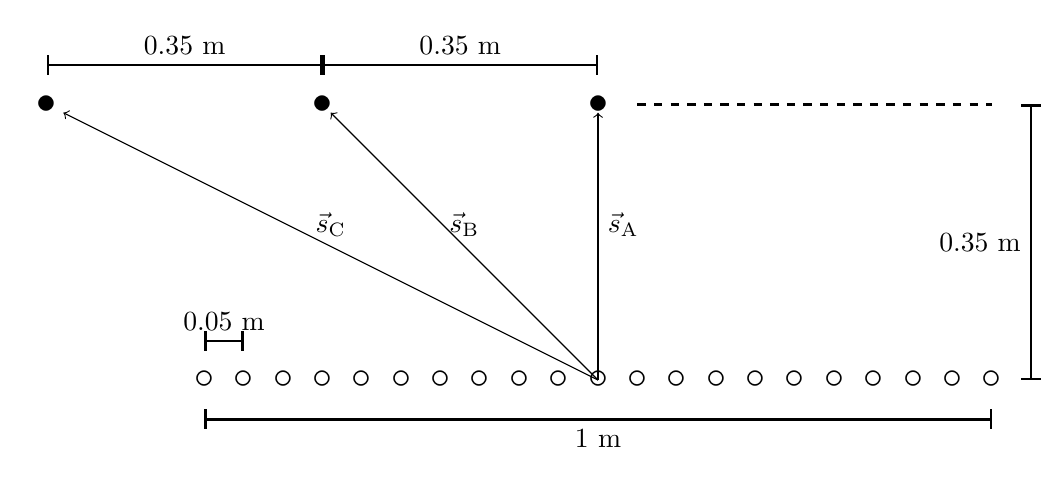
\begin{tikzpicture}[scale=10]
% Parameters
\def\radius{0.1};
\def\arrowScale{0.97};
\def\offset{0.05};

\def\micSpacing{1};
\def\micIncrement{0.05};
\def\micL{-0.5*\micSpacing};
\def\micR{0.5*\micSpacing};

\def\sourceAX{0};
\def\sourceBX{-0.35};
\def\sourceCX{-0.7};
\def\sourceY{0.35};

\pgfmathsetmacro\sourceAAzimuth{-atan(\sourceAX/\sourceY)}
\pgfmathsetmacro\sourceBAzimuth{-atan(\sourceBX/\sourceY)}
\pgfmathsetmacro\sourceCAzimuth{-atan(\sourceCX/\sourceY)}

\def\arcRadius{0.25};
\pgfmathsetmacro\arcAY{cos(-\sourceAAzimuth/2)*\arcRadius}
\pgfmathsetmacro\arcAX{sin(-\sourceAAzimuth/2)*\arcRadius}
\pgfmathsetmacro\arcBY{cos(-\sourceBAzimuth/2)*\arcRadius}
\pgfmathsetmacro\arcBX{sin(-\sourceBAzimuth/2)*\arcRadius}
\pgfmathsetmacro\arcCY{cos(-\sourceCAzimuth/2)*\arcRadius}
\pgfmathsetmacro\arcCX{sin(-\sourceCAzimuth/2)*\arcRadius}

% Coordinate system
%\draw[ultra thick,->] (0,0) -- (0,\radius);
%\draw[ultra thick,->] (0,0) -- (-\radius,0);

% Arrows
\node at (\sourceAX,\sourceY){\Large $\bullet$}; % source A
\node at (\sourceBX,\sourceY){\Large $\bullet$}; % source B
\node at (\sourceCX,\sourceY){\Large $\bullet$}; % source C
\draw[->] (0,0) -- (\arrowScale*\sourceAX,\arrowScale*\sourceY) node[above right, pos=0.5]{$\vec{s}_\textrm{A}$}; % source A
\draw[->] (0,0) -- (\arrowScale*\sourceBX,\arrowScale*\sourceY) node[above, pos=0.5]{$\vec{s}_\textrm{B}$}; % source B
\draw[->] (0,0) -- (\arrowScale*\sourceCX,\arrowScale*\sourceY) node[above, pos=0.5]{$\vec{s}_\textrm{C}$}; % source C

% Arcs
%\draw[domain=90:(90+\sourceBAzimuth)] plot ({\arcRadius*cos(\x)}, {\arcRadius*sin(\x)});
%\node at (1.15*\arcBX,1.15*\arcBY){$\varphi_\textrm{B}$};

% Mic positions
\foreach \i in {0,...,20}
{
\node at (\micL + \i*\micIncrement,0){\Large $\circ$};
}
%\node at (0,0){\Large $\circ$};
%\node at (\micL,0){\Large $\circ$};
%\node at (\micR,0){\Large $\circ$};

% Length measurements
\draw[thick,|-|] (\micL,-\offset) -- (\micR,-\offset) node[below, pos=0.5]{$1$~m};
\draw[thick,|-|] (\micL,\offset) -- (\micL+\micIncrement,\offset) node[above, pos=0.5]{$0.05$~m};
\draw[thick,|-|] (\micR+\offset,0) -- (\micR+\offset,\sourceY) node[left, pos=0.5]{$0.35$~m};
\draw[thick,dashed,-] (\micIncrement,\sourceY) -- (\micR,\sourceY);
\draw[thick,|-|] (\sourceCX,\sourceY+\offset) -- (\sourceBX,\sourceY+\offset) node[above, pos=0.5]{$0.35$~m};
\draw[thick,|-|] (\sourceBX,\sourceY+\offset) -- (\sourceAX,\sourceY+\offset) node[above, pos=0.5]{$0.35$~m};

\end{tikzpicture}
  \caption[Diagram of the experimental setup used for validation.]{
  Diagram of microphone positions (empty circles) and source positions (filled circles).}
  \label{fig:10_Experimental_Validation:Experimental_Setup}
\end{figure}

For each microphone spacing $\Delta \in [0.1,1]$~m (taken in increments of $0.1$~m) and each source position,
we estimate, using both the weighted average and proposed navigational methods (described in \secreftwo{sec:03_Navigation_Techniques:XF_Technique}{sec:08_Proposed_Method:Proposed_Techniques}, respectively), the ambisonics impulse response at each intermediate microphone position.
In all cases and at each intermediate position, we compute the following ``measured'' values: level, $\lambda'$; ABSE, $\eta'(f_c)$; localization vector,  $\vec{\nu}'$; and diffuseness, $\Psi'(f)$.
To better match the measurements, which were taken using the Eigenmike, we modify the near-field compensation filters given by \eqnref{eq:02_Acoustical_Theory:NearField_HPF} to use the following corner frequencies: $f_2 = 400$~Hz, $f_3 = 1$~kHz, and $f_4 = 1.8$~kHz (no filters are applied for orders $l = 0,1$), as specified in the EigenUnits user manual \citep[section 4.3]{EigenUnitsManual2018}.

\section{Results and discussion}\label{sec:10_Experimental_Validation:Results}
Given the simulated and measured ABSE spectra (as defined in \secref{sec:04_Auditory_Models:Coloration_Metrics:ABSE}), we first compute the discrepancy, $d_\eta(f_c) = |\eta(f_c) - \eta'(f_c)|$, for each navigation method, source position, microphone spacing, and intermediate microphone position (a total of $1 + (\Delta/0.05)$ distinct positions for each microphone spacing).
We then average, in a single operation, these discrepancies over every combination of microphone spacing and \textit{strictly interior} (i.e., $|u_y| < \Delta/2$) intermediate microphone position (note that this is only $(\Delta/0.05) - 1$ positions per spacing).

\begin{figure}[t]
\centering
  \includegraphics[width = 0.55\textwidth]{10_experimental_validation/figures/scharer2009_fullexp_F.eps}
  \caption[Experimental discrepancies in coloration spectra.]{
  Average discrepancies in ABSE spectra between simulations and measurements.
  Discrepancies are plotted for both the weighted average method (denoted by filled symbols) and the proposed method (empty symbols),
  as well as for each source: A ($\triangle$), B ($\square$), and C ($\bigcirc$).
  For each source and method combination, a thin black line connects the data points, while a thick black line indicates the average over all six curves.}
  \label{fig:10_Experimental_Validation:ABSE_Freq_Discrepancy}
\end{figure}

In \figref{fig:10_Experimental_Validation:ABSE_Freq_Discrepancy}, we plot, as a function of frequency, these average discrepancies in ABSE between the simulations and measurements for each navigation method and source position.
From this plot, we see that the simulations consistently match, within $\sim1$~dB, the physical measurements over a frequency range of approximately $150$~Hz to $10$~kHz.
The sharp increase in discrepancy at high frequencies can be explained by spatial aliasing,
a well-known effect which we do not model in our simulations (see \citet{Rafaely2005a}, for example).
The gradual increase in discrepancy at low frequencies, however, is explained by a combination of a) mismatches between the near-field compensation filters, b) non-anechoic conditions below $\sim425$~Hz, and c) low-frequency ambient noise in the measurements.

\begin{figure}[t]
\centering
  \includegraphics[width = 0.55\textwidth]{10_experimental_validation/figures/merimaa2005_fullexp_F.eps}
  \caption[Experimental discrepancies in diffuseness spectra.]{
  Average discrepancies in diffuseness spectra between simulations and measurements.
  Discrepancies are plotted for both the weighted average method and the proposed method,
  as well as for each source.
  For each source and method combination, a thin black line connects the data points, while a thick black line indicates the average over all six curves.}
  \label{fig:10_Experimental_Validation:Diffuseness_Freq_Discrepancy}
\end{figure}

In \figref{fig:10_Experimental_Validation:Diffuseness_Freq_Discrepancy}, we plot, as a function of frequency, similarly averaged discrepancies in diffuseness (as defined in \secref{sec:04_Auditory_Models:Diffuseness_Parameter}) between the simulations and measurements, given by $d_\Psi(f) = |\Psi(f) - \Psi'(f)|$, for each navigation method and source position.
From this plot, we again see that the simulations consistently match, within $\sim0.1$, the physical measurements over a frequency range of approximately $300$~Hz to $10$~kHz.
Again, spatial aliasing at high frequencies and the other effects mentioned above at low frequencies are evident.

\begin{figure}[t]
    	\centering
    	\begin{subfigure}[b]{0.49\textwidth}
		\includegraphics[width=\textwidth]{10_experimental_validation/figures/audibleEnergy_fullexp_D.eps}
		\caption{Level discrepancies}
		\label{fig:10_Experimental_Validation:MAE_Delta_Discrepancy}
    	\end{subfigure}
	\hfill
	\begin{subfigure}[b]{0.49\textwidth}
		\includegraphics[width=\textwidth]{10_experimental_validation/figures/scharer2009_fullexp_D.eps}
		\caption{ABSE discrepancies}
		\label{fig:10_Experimental_Validation:ABSE_Delta_Discrepancy}
    	\end{subfigure}
	
	\vspace{0.5cm}
	\begin{subfigure}[b]{0.49\textwidth}
		\includegraphics[width=\textwidth]{10_experimental_validation/figures/tylka2017_fullexp_D.eps}
		\caption{Localization discrepancies}
		\label{fig:10_Experimental_Validation:rPE_Delta_Discrepancy}
    	\end{subfigure}
	\hfill
	\begin{subfigure}[b]{0.49\textwidth}
		\includegraphics[width=\textwidth]{10_experimental_validation/figures/merimaa2005_fullexp_D.eps}
		\caption{Diffuseness discrepancies}
		\label{fig:10_Experimental_Validation:Diffuseness_Delta_Discrepancy}
    	\end{subfigure}
	
    	\caption[Experimental discrepancies for each microphone spacing.]{
	Discrepancies in level (top left panel), ABSE (top right), localization direction (bottom left), and diffuseness (bottom right), all plotted for each microphone spacing.
	The ABSE and diffuseness discrepancy spectra were first averaged over $[0,10]$~kHz.
  See \figref{fig:10_Experimental_Validation:ABSE_Freq_Discrepancy} for a description of the lines and symbols used.}
    	\label{fig:10_Experimental_Validation:Delta_Discrepancies}
\end{figure}

In \figref{fig:10_Experimental_Validation:MAE_Delta_Discrepancy}, we plot, now as a function of microphone spacing, the average discrepancies in level (as defined in \secref{sec:04_Auditory_Models:Audible_Energy}), given by $d_\lambda = |\lambda - \lambda'|$, where the average is taken over \textit{all} intermediate microphone positions for each microphone spacing.
From this plot, we see that the level discrepancies are consistently smaller than 2~dB, with a very slight and gradual increase with increasing microphone spacing.

In \figref{fig:10_Experimental_Validation:ABSE_Delta_Discrepancy}, we plot the average discrepancies in ABSE, where two averages are taken: first over all frequencies $f_c \in [0,10]$~kHz and subsequently over all strictly interior intermediate microphone positions.
From this plot we see that the discrepancy between simulation and measurement is consistently smaller than $1$~dB, again with a very slight and gradual increase with increasing microphone spacing.

Given the simulated and measured localization directions (from the localization model described in \secref{sec:05_Proposed_Models:Localization_Model}), we next compute the discrepancy, $d_\nu = \cos^{-1} \left( \hat{\nu} \cdot \hat{\nu}' \right)$, for each navigation method, source position, microphone spacing, and intermediate microphone position.
In \figref{fig:10_Experimental_Validation:rPE_Delta_Discrepancy}, we plot, as a function of microphone spacing, averages of these discrepancies over all strictly interior intermediate microphone positions.
From this plot we see that the discrepancy between simulation and measurement is consistently smaller than $5^\circ$, with an average value of approximately $3.5^\circ$, and does not vary significantly with microphone spacing.

Finally, in \figref{fig:10_Experimental_Validation:Diffuseness_Delta_Discrepancy}, we plot the average discrepancies in diffuseness, where again two averages are taken: first over all frequencies $f \in [0,10]$~kHz and subsequently over all strictly interior intermediate microphone positions.
From this plot we see that the discrepancy between simulation and measurement is consistently smaller than $0.1$ and does not vary significantly with microphone spacing.

Taken together, \figrefthru{fig:10_Experimental_Validation:ABSE_Freq_Discrepancy}{fig:10_Experimental_Validation:Delta_Discrepancies} further suggest that the discrepancies between simulations and measurements do not depend significantly on navigational method or source position.

\section{Conclusions}\label{sec:10_Experimental_Validation:Conclusions}
In order to validate our numerical simulations, we conducted a set of acoustical measurements, as described in \secref{sec:10_Experimental_Validation:Experiments}, taken over a subset of the simulated conditions presented in \chapref{chap:08_Proposed_Method}.
Results of these measurements are in good agreement with those of the simulations, indicating that our simulations are indeed representative of reality.
In particular, spectral error discrepancies are consistently smaller than $1$~dB and diffuseness discrepancies are consistently smaller than $0.1$ across all frequencies within approximately $300$~Hz to $10$~kHz.%
\footnote{The significant discrepancies observed at high frequencies can be explained by spatial aliasing, an effect which we do not currently account for in our simulations, but could potentially be incorporated in the future with a simple model based on the geometrical arrangement of capsules on the spherical microphone array used in the measurements.}
Additionally, level discrepancies are consistently within $2$~dB and localization direction discrepancies are consistently within $5^\circ$ ($3.5^\circ$ on average) across all microphone spacings.
A more comprehensive validation of our simulation framework could consider alternative navigational methods and span wider ranges of microphone spacings and source positions.
However, as expected, the present results suggest that the observed discrepancies (and therefore the fidelity of the simulations) do not depend significantly on the navigational method, microphone spacing, or source position.

\section*{Acknowledgements}
The ambisonics room impulse responses were recorded using the Eigenmike by mh Acoustics \citep{EigenmikeURL}.
This work was originally submitted by \citet[section 6]{TylkaChoueiri2019b} to \textit{The Journal of the Audio Engineering Society}.
%%%% CONCLUSIONS %%%%
\chapter{Conclusions}\label{chap:11_Conclusions}
% Summary of contributions

In this thesis, we have explored the problem of, and state-of-the-art methods for, virtual navigation of ambisonics-encoded sound fields, with a particular emphasis on the challenges and perceptual penalties related to the region of validity restriction.%
\footnote{Recall that the region of validity restriction states that the spherical-harmonic description of a sound field, as captured by an ambisonics microphone, is only valid in a spherical region around the microphone that extends up to the nearest source or scattering body, i.e., only in the free-field.
See \secref{sec:02_Acoustical_Theory:Helmholtz_Equation} for more details.}
The primary contributions comprising this work can be summarized as follows:
\begin{itemize}
\item we have proposed, for the purpose of evaluating and comparing navigational methods, a suite of perceptually-relevant objective metrics and models for sound level, spectral coloration, perceived localization, and diffuseness (as enumerated in \secref{sec:06_Simulation_Framework:Metrics} and defined in \chapreftwo{chap:04_Auditory_Models}{chap:05_Proposed_Models});
\item in particular, we have developed, and subsequently validated through subjective listening experiments, auditory models for perceived localization and coloration (see \chapref{chap:05_Proposed_Models});
\item we have implemented and experimentally validated a numerical simulation framework with which one can comprehensively characterize the performance of a given navigational method (see \chapreftwo{chap:06_Simulation_Framework}{chap:10_Experimental_Validation});
\item we have provided critical reviews of existing extrapolation- and interpolation-based navigational methods (see \secreftwo{sec:07_Characterization_Extrapolation:Introduction}{sec:08_Proposed_Method:Introduction}, respectively), through which we have identified a number of common issues facing those methods;
\item we have characterized and compared the performance of linear extrapolation methods (see \chapref{chap:07_Characterization_Extrapolation}) as well as linear and parametric interpolation methods (see \chapreftwo{chap:08_Proposed_Method}{chap:09_Thiergart_Comparison});
\item through these evaluations, we have explored the particular penalties associated with violating the region of validity restriction (see \chapreftwo{chap:07_Characterization_Extrapolation}{chap:08_Proposed_Method});
\item we have proposed a parametric interpolation method which ensures that this restriction is not violated (see \chapref{chap:08_Proposed_Method}); and
\item we have identified practical guidelines with which future researchers might choose between the parametric navigational methods considered here, depending on their intended application (see \chapref{chap:09_Thiergart_Comparison}).
\end{itemize}
In this final chapter, we summarize the major findings that have resulted from this work, synthesize our earlier findings related to violating the region of validity restriction into broader insights, identify additional practical guidelines with which to choose between all of the methods considered here, and finally propose some possible avenues for further research.

\section{Summary of major findings}
Below, we summarize the four major findings that have resulted from this work.

%% Ch 5 - new models
\paragraph{Perceived localization and coloration can be accurately predicted directly from ambisonics impulse responses.}
In \chapref{chap:05_Proposed_Models}, we developed auditory models to predict, from an ambisonics impulse response, the perceived localization of a source and the perceived spectral coloration compared to a reference signal.
Traditionally, these attributes are estimated using binaural models, the predictions of which are necessarily confounded by the adopted ambisonics-to-binaural rendering approach.
Our proposed localization model extends the precedence-effect-based energy vector model of \citet{Stitt2016} by providing a pre-processing front end that extracts, from the ambisonics impulse response, a finite set of spatially- and temporally-distinct ``wavelets,'' all of which are then fed into the energy vector model in order to compute a single perceived source direction (see \secref{sec:05_Proposed_Models:Localization_Model} for more details).
%Our model essentially consists of that model and a pre-processing front end, which breaks the ambisonics impulse response into a finite set of discrete sounds with directions-of-arrival given by a plane-wave decomposition, times-of-arrival found by splitting each plane-wave impulse response into distinct ``wavelets'' identified via thresholding, and signal amplitudes given by a gammatone filter bank applied to each wavelet (see \secref{sec:05_Proposed_Models:Localization_Model} for more details).
We validated our model through a comparison with the results of a subjective localization experiment, in which subjects were asked to judge source directions for a set of measured and interpolated ambisonics impulse responses (rendered binaurally with head-tracking).
This comparison revealed 1) that our model performs comparably, if not superior, to the well-established binaural localization model of \citet{Dietz2011} and 2) that the \textit{structure} of our model is indeed valid, as the model was able to achieve (after optimizing its free parameters using the data) an average prediction error of only $3.67^\circ$ and a correlation coefficient between the predictions and data of $0.85$.

Our coloration model comprised a linear combination of two distinct metrics of spectral distortion: the range (in dB) of the difference spectrum after critical-band filtering (see \secref{sec:04_Auditory_Models:Coloration_Metrics:ABSE}) and the average depth of narrowband notches (see \secref{sec:04_Auditory_Models:Coloration_Metrics:Epk}).
We validated this model through a comparison with the results of a subjective coloration experiment, in which subjects were asked to rate spectral differences between modified and reference ambisonics impulse responses (rendered binaurally).
This comparison revealed that the two metrics included in the model are both dominant factors in human perception of coloration, such that each may serve independently as a useful measure of perceptible spectral coloration.

%% Ch 7 - extrapolation errors
\paragraph{Level and localization performance of linear extrapolation methods degrades for near-field sources.}
In \chapref{chap:07_Characterization_Extrapolation}, we characterized and compared, through numerical simulations and in terms of our proposed suite of objective metrics, the performance of two linear extrapolation methods: plane-wave translation and ambisonics translation (reviewed in \secreftwo{sec:03_Navigation_Techniques:PW_Technique}{sec:03_Navigation_Techniques:SR_Technique}, respectively).
An analysis of the plane-wave translation method alone revealed a clear advantage to matching the number of plane-wave terms, when computed via the ``beamforming'' plane-wave decomposition method, to the number of ambisonics signals.

With this implementation, the plane-wave translation method was shown to accurately reproduce both the level and localization of far-field sources.
In contrast, the ambisonics translation method was shown to incur significant errors in both level and coloration, which increase steadily with translation distance, due primarily to the low-pass-like roll-off of high-frequency energy seen in the frequency response induced by the method (see \figref{fig:07_Characterization_Extrapolation:Azimuth_Dependence:SRE}, for example).
In our analysis, we also showed that the performance of both methods degrades for near-field sources, since such sources lead to violations of the region of validity restriction.
In particular, when reproducing a near-field source, both methods incurred significant localization errors as well as a deficiency in the reproduced sound level.

%% Ch 8 - proposed method
\paragraph{Parametric exclusion of invalid microphones improves coloration performance and localization accuracy.}
In \chapref{chap:08_Proposed_Method}, we characterized and compared the performance of our proposed parametric interpolation method to that of a benchmark linear interpolation method.
Our method ensures, using the known or inferred positions of any near-field sources, that the region of validity restriction is not violated by excluding from the interpolation calculation those microphones that do not provide a valid description of the sound field at the position of the listener.
In contrast, the benchmark method simply computes a per-channel weighted-average across the microphones, with weights determined by the position of the listener (see \secref{sec:03_Navigation_Techniques:XF_Technique} for more details).

Through our analysis, we showed that the benchmark method introduces 1) large localization errors for near-field sources due to the precedence effect imposed by the nearest microphone to the source, 2) significant spectral errors due to comb-filtering, and 3) excessive diffuseness due to conflicting localization information between the two microphones.
The proposed method, on the other hand, achieves significantly improved localization performance, smaller spectral errors, and virtually exact diffuseness, all as a consequence of excluding the invalid microphone.

%% Ch 9 - time-frequency method
\paragraph{The time-frequency analysis method improves localization but degrades coloration performance in applications with a sparse microphone array and intimate sources.}
In \chapref{chap:09_Thiergart_Comparison}, we compared the parametric time-frequency interpolation method of \citet{Thiergart2013} to our proposed parametric method and, using trends observed in the data, we presented practical guidelines with which to choose between the two methods.
In order to distinguish between various potential applications, we first defined three practically-relevant ``axes'': the sparsity of the microphone array, the intimacy (i.e., proximity) of the sound sources, and the complexity of the sound field (see \secref{sec:09_Thiergart_Comparison:Conclusions} for definitions of these terms).
For applications spanning the first two axes, we also determined domains over which each method yields \textit{accurate and superior} performance, compared to the other method, in terms of spectral coloration and localization accuracy (see \figref{fig:09_Thiergart_Comparison:Region_Plots} and corresponding text).
%First, the \textit{sparsity} of the microphone array compares the size of the desired navigable region to the number of ambisonics microphones available. % u and \Delta/2 for P = 1,2
%Second, the \textit{intimacy} of the sound sources compares the average source distance (from the origin) to the size of the microphone array (or the size of the navigable region for a single microphone). % 1/\gamma
%Finally, the \textit{complexity} of the sound field refers to the number of sources and reflecting surfaces in the sound field.

According to the results of our analysis, for most applications with a sparse microphone array and with intimate sources, the time-frequency method will achieve superior localization performance, whereas the proposed method will incur less spectral coloration.
Additionally, for intimate sources, the time-frequency method will likely better convey source distance information due its accurate reproduction of sound level (which is a dominant cue in human perception of source distance \citep[section 3.1.1]{Zahorik2005}).%
\footnote{This potential benefit may be negated by the coloration introduced by the time-frequency method (see \figref{fig:09_Thiergart_Comparison:Spectral_Errors:Thiergart}), since spectrum is also a dominant perceptual cue for source distance \citep[section 3.1.3]{Zahorik2005}.
However, while the relationship between level and perceived distance is rather straightforward, the relationship between coloration and distance is less so, since only certain types of coloration (e.g., a high-shelf-like filter mimicking atmospheric absorption) are likely to influence perceived distance.}
For distant sources, on the other hand, the proposed method offers a marginal improvement over the time-frequency method in both spectral coloration and source localization.
Finally, the time-frequency method is likely preferable for acoustically simple sound fields, as it will yield superior localization accuracy and since its deficiency in diffuseness may not be noticeable, whereas, for acoustically complex sound fields, the proposed method is likely preferable due to its accurate reproduction of diffuseness.

\section{Penalties related to the region of validity}
% From Ch. 1 objectives: we seek broader insights into the nature of the penalties incurred by violating the region of validity restriction

In \chapreftwo{chap:07_Characterization_Extrapolation}{chap:08_Proposed_Method}, we drew separate insights for extrapolation and interpolation methods, respectively, regarding the penalties incurred by violating the region of validity restriction.
Here, we synthesize these findings into broader insights on this subject.

% bad localization due to drastic changes in direction geometry
First, we note that, in the presence of a near-field source, both extrapolation methods as well as the weighted-average interpolation method exhibit extremely large localization errors ($e_\nu > 30^\circ$) for translation distances larger than approximately $0.5$~m (see \figrefthree{fig:07_Characterization_Extrapolation:Localization_Errors:PWT}{fig:07_Characterization_Extrapolation:Localization_Errors:SRE}{fig:08_Proposed_Method:Localization_Errors:XF}).
This is primarily a geometric effect: as the listener traverses the navigable region (as defined in \secref{sec:06_Simulation_Framework:Geometry} for both the extrapolation and interpolation geometries), the intended source direction can change drastically, in particular when comparing listener positions inside and outside of the region of validity.
Evidently, none of these linear methods (extrapolation and weighted-average interpolation) can adequately compensate for the changing intended direction of the source as the listener moves.
However, both of the parametric interpolation methods considered in this thesis ensure, by construction, that the region of validity restriction is not violated and, consequently, they both achieve significantly improved localization errors under the same conditions (see \figref{fig:09_Thiergart_Comparison:Localization_Errors}).

% excessive diffuseness for interpolation methods due to conflicting localization information
A related error exhibited by the weighted-average interpolation method is the excessive diffuseness in the reproduced sound due to the conflicting localization information captured by the microphones for a near-field source (see \figref{fig:08_Proposed_Method:Diffuseness_Errors:XF}).
Although the extrapolation methods do not exhibit this error, we expect that any other interpolation method that does not compensate for the conflicting localization information will suffer from this error as well.

% bad levels due to drastic changes in distance geometry
Another common error introduced when the region of validity restriction is violated is that the reproduced sound level is several dB too low (see \figrefthree{fig:07_Characterization_Extrapolation:Level_Errors:PWT}{fig:07_Characterization_Extrapolation:Level_Errors:SRE}{fig:08_Proposed_Method:Level_Errors:XF}).
This too is largely a geometric effect, since none of the linear methods considered here are able to adequately increase the reproduced level as the listener navigates very close to a source.
Indeed, even our proposed method, which ensures that the region of validity restriction is not violated, exhibits a very similar error (see \figref{fig:08_Proposed_Method:Level_Errors:Hybrid}) since it does not amplify the microphone signals as the listener approaches a source.
Only the parametric time-frequency method (described in \secref{sec:03_Navigation_Techniques:Thiergart_Method}), which models the sound field with a virtual point source at the estimated position of the real source, is able to adequately reproduce the sound levels of near-field sources (see \figref{fig:09_Thiergart_Comparison:Level_Errors:Thiergart}).

% summarize
In sum, the penalties introduced by violating the region of validity restriction relate primarily to the drastic changes in the apparent geometry of the sound field as the listener navigates.
In particular, methods that do not account for the region of validity restriction are unable to adequately reproduce for near-field sources both the level changes due to longitudinal translations (i.e., towards or away from the source) and the localization changes due to lateral translations (perpendicular to the direction of the source).
Additionally, for interpolation methods that do not account for the region of validity restriction, the conflicting apparent geometries captured by the different microphones will incur not only degraded localization accuracy but also an excessive diffuseness in the reproduced sound.

\section{Practical implications}
% From Ch. 1 objectives: we identify considerations regarding the suitability of each method to various applications

In \secref{sec:09_Thiergart_Comparison:Conclusions}, we identified several general principles with which to choose between the two parametric interpolation methods considered in that chapter for various potential applications.
As mentioned above, we discussed these applications in terms of three axes: the sparsity of the microphone array, the intimacy of the sound sources, and the complexity of the sound field. % (see \figref{fig:09_Thiergart_Comparison:Practical_Axes}).
Building on that discussion, here, we identify several additional principles for choosing between all of the methods considered in this work:
\begin{enumerate}
% sparsity axis
\item[1a.] With a sparse microphone array, the weighted-average method will achieve a marginal improvement in spectral coloration over the time-frequency method.
The ambisonics translation method should be avoided as it will incur significant level and spectral errors for even a moderately-sized (e.g., $\sim0.5$~m) navigable region.
\item[1b.] With a dense microphone array, the weighted-average method will yield the smallest localization errors, although none of the methods considered here will achieve particularly accurate localization unless the sources are very far away.
%This is an area for future development.
% intimacy axis
\item[2a.] When recording primarily intimate sources, all of the linear methods will incur significant localization errors and the weighted-average method in particular will introduce excessive diffuseness.
\item[2b.] When recording primarily distant sources, the plane-wave translation method will yield accurate reproductions of sound level, localization, and diffuseness with just a single ambisonics microphone.
The weighted-average method will yield similarly accurate reproductions of these metrics.
% complexity axis
\item[3a.] For an acoustically complex sound field, the linear methods may be advantageous since 1) by construction, they can trivially accommodate multiple sources and 2) the extrapolation methods will accurately reproduce diffuseness, and the additional diffuseness introduced by the weighted-average method for intimate sources may not be noticeable.
\item[3b.] For an acoustically simple sound field, however, the excessive diffuseness introduced by the weighted-average method for near-field sources may be particularly distracting.
\end{enumerate}

As an extension of the analysis presented in \secref{sec:09_Thiergart_Comparison:Conclusions} (and summarized above), here we determine, for all of the methods considered in this thesis, the domains (across array sparsity and source intimacy and in terms of coloration and localization) over which each method yields both \textit{accurate and superior} performance, where we define ``accurate'' performance as achieving spectral errors of $\rho_\eta < 3$~dB and localization errors of $e_\nu < 10^\circ$.
These domains are sketched in \figref{fig:11_Conclusions:Region_Plots}.

\begin{figure*}[t]
	\centering
	\begin{subfigure}[b]{0.49\textwidth}
		\includegraphics[width=\textwidth]{11_conclusions/figures/Coloration_Region_Plot}
		\caption{Coloration}
		\label{fig:11_Conclusions:Region_Plots:Coloration}
	\end{subfigure}
	\hfill
	\begin{subfigure}[b]{0.49\textwidth}
		\includegraphics[width=\textwidth]{11_conclusions/figures/Localization_Region_Plot}
		\caption{Localization}
		\label{fig:11_Conclusions:Region_Plots:Localization}
	\end{subfigure}
	
	\caption[Region plots of practical applicability of each navigational method.]{
	Region plots illustrating accurate and superior methods in terms of spectral coloration (left panel) and localization accuracy (right) across practical applications with varying microphone array sparsity (horizontal axis) and sound source intimacy (vertical).
	The gray filled regions correspond to the proposed method;
	the coarsely-hatched regions correspond to the time-frequency method of \citet{Thiergart2013};
	the finely-hatched regions correspond to the weighted-average interpolation method;
	and the dark gray filled region corresponds the plane-wave translation method (labeled ``PWT''), in addition to the proposed method.
	Regions that are both filled and hatched indicate that the methods perform comparably;
	empty regions indicate that none of the methods satisfy the specified error limit.}
	\label{fig:11_Conclusions:Region_Plots}
\end{figure*}

From \figref{fig:11_Conclusions:Region_Plots:Coloration}, we first note that no method offers any domain of accurate coloration performance that is distinct from that of the proposed method.
(Note that neither of the extrapolation methods offer sufficiently accurate coloration performance to appear in that plot.)
Furthermore, for localization (see \figref{fig:11_Conclusions:Region_Plots:Localization}), we see that the regions of accurate performance for the two linear methods shown are contained within that of the proposed method.
Only the time-frequency method offers a distinct (from the proposed method) practical domain of accurate localization performance: in applications with a sparse microphone array and intimate sources.

From these figures, we also note that the weighted average method, similarly to the proposed method, offers accurate performance in both coloration and localization in applications with a sparse microphone array and distant sources.
This is unsurprising, since for distant sources (i.e., since the region of validity is not violated), the proposed method performs a very similar interpolation calculation to that done by the weighted average method (see \secref{sec:08_Proposed_Method:Hybrid_Technique}).

% some more general results across methods, not necessarily along the axes
Of all of the methods considered in this thesis, either of the parametric interpolation methods is generally preferable over any of the linear methods for most applications, since, except where noted above, the parametric methods tend to outperform the linear ones.
In particular, in most applications, both of the parametric methods considered here achieve significantly improved localization accuracy compared to the linear methods.
The results presented in this thesis also show that any interpolation method will yield significantly improved spectral errors compared to either of the extrapolation methods.

% some sort of concluding thing
It should be emphasized that the existing body of literature relating to virtual navigation of ambisonics-encoded sound fields has been largely numerical in nature (and the present thesis is no exception), so this particular field of research is notably lacking in practical experience.
Consequently, it is our hope that the guidelines enumerated above (as well as those in \secref{sec:09_Thiergart_Comparison:Conclusions}) will facilitate more real-world implementations of the navigational methods considered in this thesis.
Ideally, future experimental investigations and subjective assessments of these (and other) methods will further illuminate the deficiencies of the existing methods and thereby inform the development of novel ones.

\section{Future work}
% explore different sound fields / source configurations
The analyses presented in this thesis provide a baseline set of characterizations of the various navigational methods considered here.
One avenue for further research is to consider additional types of simulated sound fields, such as those consisting of multiple sources, directional sources, and/or reflective surfaces.
Parametric methods in particular warrant additional analyses to establish their performance in the presence of multiple sources, which may cause deviations from the results published here.
Furthermore, in immersive applications with intimate sources, the ability of a navigational method to accurately capture and reproduce the directivities of those sources may be critical, but this issue is largely unexplored in the literature (with the exception of the study by \citet{Wakayama2017}).
%Since, by construction, the time-frequency method models the incident sound field as a collection of omnidirectional point sources, it might be expected that this method will be unable to accurately reproduce any other directivity.

% explore different methods / microphone configurations
Additionally, in the present thesis, we considered only a subset of all existing navigational methods (see \tabref{tab:01_Introduction:Methods}).
Future investigations should therefore consider alternative methods, such as the parametric extrapolation methods of \citet{Wakayama2017} and \citet{Plinge2018}, which, like the parametric interpolation methods considered in this thesis, should be able to circumvent the region of validity restriction.
One might also extend the characterizations of the interpolation methods considered here to two-dimensional array configurations, such as an equilateral triangle or a square (cf.~\citet{Mariette2010} and \citet{Bates2018}, respectively).

% explore additional metrics / models
Future research might also seek to enlarge or improve the set of objective auditory metrics and models which we have employed throughout this thesis.
For example, although errors in the reproduced sound level are likely sufficient to produce errors in distance perception \citep[section 3.1.1]{Zahorik2005}, it may be useful to develop a dedicated model for perceived source distance, perhaps based on the known formula for distance coding of point-sources (see \eqnref{eq:02_Acoustical_Theory:PointSource_An}).
Additionally, subjective evaluations of stimuli with varying diffuseness should be conducted in order to establish a perceptual threshold for audibility of diffuseness errors.

% sensitivity analysis
Finally, although we have endeavored to make the analyses presented in this thesis practically relevant, we did not consider any sensitivities of the navigational methods to small errors that may arise in practice.
Consequently, any degradations in performance incurred due to errors in microphone placement or orientation should be quantified.
Additionally, as both of the parametric methods considered here require estimates of the positions of sources, the impact of any estimation errors (e.g., triangulation errors due to noise) on the performance of those methods should be explored.

\appendix % all chapters following will be labeled as appendices
%%%% NAVIGATION FILTERS %%%%
\chapter{Algorithms for computing ambisonics translation filters}\label{chap:A1_Navigation_Filters}
In this appendix, we distill and reproduce the necessary algorithms for computing the ambisonics translation filters introduced in \secref{sec:02_Acoustical_Theory:Ambisonics_Translation}.
These algorithms are also described by \citet[chapter 3]{GumerovDuraiswami2005} for complex-valued spherical harmonics and by \citet[chapter III]{Zotter2009PhD} for both complex- and real-valued spherical harmonics.
The translation operation consists of three steps:
\begin{enumerate}
\item rotating the coordinate system to align the $z$-axis with the desired translation direction,
\item translating along the new $z$-axis, and
\item rotating the coordinate system back to its original orientation.
\end{enumerate}
In \secref{sec:A1_Navigation_Filters:Recurrence_Coefficients}, we present recurrence coefficients which will be used both
in \secref{sec:A1_Navigation_Filters:Rotation_Matrices} to derive the rotation matrices needed to align the $z$-axis and
in \secref{sec:A1_Navigation_Filters:Coaxial_Filters} to derive the coefficient matrix used to translate along the $z$-axis.
We then show in \secref{sec:A1_Navigation_Filters:Translation_Filters} how to combine these individual matrices in order to compute the coefficients matrix for an arbitrary translation.

\section{Recurrence coefficients}\label{sec:A1_Navigation_Filters:Recurrence_Coefficients}
The $a$ and $b$ recurrence coefficients are given, respectively, by \citep[Eq.~(145)]{Zotter2009PhD}
\begin{equation}\label{eq:A1_Navigation_Filters:Recurrence_Coefficient_a}
a_l^m =
\begin{cases}
  \displaystyle \sqrt{\frac{(l - |m| + 1) (l + |m| + 1)}{(2 l + 1) (2 l + 3)}} & \text{for}~l \geq 0~\text{and}~0 \leq |m| \leq l, \\
  0 & \text{otherwise,}
\end{cases}
\end{equation}
and \citep[Eq.~(146)]{Zotter2009PhD}
\begin{equation}\label{eq:A1_Navigation_Filters:Recurrence_Coefficient_b}
b_l^m =
\begin{cases}
  \displaystyle \sqrt{\frac{(l - m - 1) (l - m)}{(2 l - 1) (2 l + 1)}} & \text{for}~l \geq 0~\text{and}~0 \leq m \leq l, \\
  \displaystyle -\sqrt{\frac{(l - m - 1) (l - m)}{(2 l - 1) (2 l + 1)}} & \text{for}~l \geq 0~\text{and}~-l \leq m < 0, \\
  0 & \text{otherwise.}
\end{cases}
\end{equation}

\section{Rotation matrices}\label{sec:A1_Navigation_Filters:Rotation_Matrices}
In this section, we derive a collection of rotation matrices, denoted by $\mathbf{Q}$, which, when applied to a set of ambisonics signals, rotate the sound field around the listener.
That is, given a column-vector of ambisonics signals $\mathbf{b}$, the rotated ambisonics signals are given by
\begin{equation}
\mathbf{b}_\text{r}(k) = \mathbf{Q} \cdot \mathbf{b}(k).
\end{equation}
Equivalently, in order to rotate the listener within the sound field, we apply the corresponding inverse rotation matrix.
That is, given ambisonics signals $\mathbf{b}$, the desired ambisonics signals for a rotated listener are given by
\begin{equation}
\mathbf{b}_\text{r}(k) = \mathbf{Q}^{-1} \cdot \mathbf{b}(k).
\end{equation}
Note that, unlike translation (as we will see in \secref{sec:A1_Navigation_Filters:Coaxial_Filters}), the rotation operation is time- and frequency-independent, so it can be performed either in the frequency domain, where $\mathbf{Q}$ is applied per frequency, or in the time domain, where $k$ then indicates the time sample.

It is convenient to note that all of the rotation matrices presented here are necessarily orthogonal, such that $\mathbf{Q}^{-1} = \mathbf{Q}^\text{T}$ \citep{Choi1999}.
Consequently, we can also achieve a rotation of the listener by
\begin{equation}\label{eq:A1_Navigation_Filters:Listener_Rotation}
\mathbf{b}_\text{r}(k) = \mathbf{Q}^\text{T} \cdot \mathbf{b}(k) \quad \iff \quad \mathbf{b}_\text{r}^\text{T}(k) = \mathbf{b}^\text{T}(k) \cdot \mathbf{Q},
\end{equation}
where $(\cdot)^\text{T}$ denotes the transpose of the argument.

We denote the elements of $\mathbf{Q}$ by $Q_{l',l}^{m',m}$ and arrange them as follows:
\begin{equation}\label{eq:A1_Navigation_Filters:Rotation_Matrix}
    \begin{blockarray}{lc|ccc|cc}
    l = & 0 & & 1 & & 2 & \cdots \\
    \begin{block}{c[c|ccc|cc]}
    l' = 0 & Q_{0,0}^{0,0} & Q_{0,1}^{0,-1} & Q_{0,1}^{0,0} & Q_{0,1}^{0,1} & Q_{0,2}^{0,-2} & \cdots \\ \cline{2-7}
     & Q_{1,0}^{-1,0} & Q_{1,1}^{-1,-1} & Q_{1,1}^{-1,0} & Q_{1,1}^{-1,1} & Q_{1,2}^{-1,-2} & \cdots \\
    l' = 1 & Q_{1,0}^{0,0} & Q_{1,1}^{0,-1} & Q_{1,1}^{0,0} & Q_{1,1}^{0,1} & Q_{1,2}^{0,-2} & \cdots \\
     & Q_{1,0}^{1,0} & Q_{1,1}^{1,-1} & Q_{1,1}^{1,0} & Q_{1,1}^{1,1} & Q_{1,2}^{1,-2} & \cdots \\ \cline{2-7}
    l' = 2 & Q_{2,0}^{-2,0} & Q_{2,1}^{-2,-1} & Q_{2,1}^{-2,0} & Q_{2,1}^{-2,1} & Q_{2,2}^{-2,-2} & \cdots \\
    \vdots & \vdots & \vdots & \vdots & \vdots & \vdots & \ddots \\
    \end{block}
    m = & 0 & -1 & 0 & 1 & -2 & \cdots \\
    \end{blockarray},
\end{equation}
such that the indices $l,m$ correspond to the columns of the matrix while $l',m'$ correspond to the rows.
Accordingly, the indices $l,m$ refer to the input ambisonics signals $\mathbf{b}$, while the indices $l',m'$ correspond to the output ambisonics signals $\mathbf{b}_\text{r}$.

%% Variable yaw
\subsection{Variable yaw rotation}
The first rotation matrix we derive is for an arbitrary azimuthal (yaw) rotation around the $z$-axis.
Given a desired rotation angle $\alpha$, we denote the corresponding rotation matrix by $\mathbf{Q}_\text{Y}(\alpha)$ (where the subscript ``$\text{Y}$'' denotes ``yaw''), with elements given by \citep[Eq.~(3.12)]{Kronlachner2014b}
\begin{equation}\label{eq:A1_Navigation_Filters:Variable_Yaw}
Q_{l',l}^{m',m}(\alpha) = 
\begin{cases}
\cos m \alpha & \text{if}~ l=l' ~\text{and}~ m=m',\\
\sin m \alpha & \text{if}~ l=l' ~\text{and}~ m=-m',\\
0 & \text{otherwise}.
\end{cases}
\end{equation} % matches code and Kronlachner
The locations of possible nonzero elements of this matrix are illustrated in \figref{fig:A1_Navigation_Filters:Variable_Yaw}.

\begin{figure}[h]
\[
    \begin{blockarray}{lc|ccc|ccccc|ccccccc}
    l= & 0 & & 1 & & & & 2 & & & & & & 3 & & & \\
    \begin{block}{l(c|ccc|ccccc|ccccccc)}
     l' = 0 & \blacksquare &  &  &  &  &  &  &  &  &  &  &  &  &  &  &  \\ \cline{2-17}
     &  & \blacksquare &  & \blacksquare &  &  &  &  &  &  &  &  &  &  &  &  \\
     l' = 1 &  &  & \blacksquare &  &  &  &  &  &  &  &  &  &  &  &  &  \\
     &  & \blacksquare &  & \blacksquare &  &  &  &  &  &  &  &  &  &  &  &  \\ \cline{2-17}
     &  &  &  &  & \blacksquare &  &  &  & \blacksquare &  &  &  &  &  &  &  \\
     &  &  &  &  &  & \blacksquare &  & \blacksquare &  &  &  &  &  &  &  &  \\
     l' = 2 &  &  &  &  &  &  & \blacksquare &  &  &  &  &  &  &  &  &  \\
     &  &  &  &  &  & \blacksquare &  & \blacksquare &  &  &  &  &  &  &  &  \\
     &  &  &  &  & \blacksquare &  &  &  & \blacksquare &  &  &  &  &  &  &  \\ \cline{2-17}
     &  &  &  &  &  &  &  &  &  & \blacksquare &  &  &  &  &  & \blacksquare \\
     &  &  &  &  &  &  &  &  &  &  & \blacksquare &  &  &  & \blacksquare &  \\
     &  &  &  &  &  &  &  &  &  &  &  & \blacksquare &  & \blacksquare &  &  \\
     l' = 3 &  &  &  &  &  &  &  &  &  &  &  &  & \blacksquare &  &  &  \\
     &  &  &  &  &  &  &  &  &  &  &  & \blacksquare &  & \blacksquare &  &  \\
     &  &  &  &  &  &  &  &  &  &  & \blacksquare &  &  &  & \blacksquare &  \\
     &  &  &  &  &  &  &  &  &  & \blacksquare &  &  &  &  &  & \blacksquare \\
    \end{block}
    m= & 0 & -1 & 0 & 1 & -2 & -1 & 0 & 1 & 2 & -3 & -2 & -1 & 0 & 1 & 2 & 3 \\
    \end{blockarray}
\]
\caption[Graphical illustration of the rotation matrix for an arbitrary yaw rotation.]{
Graphical illustration of the locations of possible nonzero elements (indicated by the $\blacksquare$ symbols) of the rotation matrix for an arbitrary yaw rotation (see \eqnref{eq:A1_Navigation_Filters:Variable_Yaw}).}
\label{fig:A1_Navigation_Filters:Variable_Yaw}
\end{figure}

%% Fixed pitch
\subsection{Fixed pitch rotation of \texorpdfstring{$\pi/2$}{pi/2}}
The second rotation matrix we derive is for a fixed upwards pitch rotation by $\pi/2$ around the $y$-axis.
We denote this matrix $\mathbf{Q}_\text{P}(\pi/2)$ (where the subscript ``$\text{P}$'' denotes ``pitch'').
As will become clear below, for some of the recurrence formulae used in this derivation, we must compute terms of the matrix beyond the maximum ambisonics order that we intend to use.
In particular, to compute $\mathbf{Q}_\text{P}(\pi/2)$ up to order $L$, we must first compute terms in the matrix up to order $2L$, as indicated below.

The procedure for computing the rotation matrix is enumerated below and illustrated symbolically in \figref{fig:A1_Navigation_Filters:Fixed_Pitch}.

\begin{figure}[h]
\[
    \begin{blockarray}{lc|ccc|ccccc|ccccccc}
    l= & 0 & & 1 & & & & 2 & & & & & & 3 & & & \\
    \begin{block}{l(c|ccc|ccccc|ccccccc)}
     l' = 0 & \blacksquare &  &  &  &  &  &  &  &  &  &  &  &  &  &  &  \\ \cline{2-17}
     &  & \boxdot &  &  &  &  &  &  &  &  &  &  &  &  &  &  \\
     l' = 1 &  &  & \blacksquare & \blacksquare &  &  &  &  &  &  &  &  &  &  &  &  \\
     &  &  & \boxminus & \boxplus &  &  &  &  &  &  &  &  &  &  &  &  \\ \cline{2-17}
     &  &  &  &  & \boxdot & \boxdot &  &  &  &  &  &  &  &  &  &  \\
     &  &  &  &  & \boxdot & \boxdot &  &  &  &  &  &  &  &  &  &  \\
     l' = 2 &  &  &  &  &  &  & \blacksquare & \blacksquare & \blacksquare &  &  &  &  &  &  &  \\
     &  &  &  &  &  &  & \boxminus & \boxplus & \boxplus &  &  &  &  &  &  &  \\
     &  &  &  &  &  &  & \boxminus & \boxminus & \boxplus &  &  &  &  &  &  &  \\ \cline{2-17}
     &  &  &  &  &  &  &  &  &  & \boxdot & \boxdot & \boxdot &  &  &  &  \\
     &  &  &  &  &  &  &  &  &  & \boxdot & \boxdot & \boxdot &  &  &  &  \\
     &  &  &  &  &  &  &  &  &  & \boxdot & \boxdot & \boxdot &  &  &  &  \\
     l' = 3 &  &  &  &  &  &  &  &  &  &  &  &  & \blacksquare & \blacksquare & \blacksquare & \blacksquare \\
     &  &  &  &  &  &  &  &  &  &  &  &  & \boxminus & \boxplus & \boxplus & \boxplus \\
     &  &  &  &  &  &  &  &  &  &  &  &  & \boxminus & \boxminus & \boxplus & \boxplus \\
     &  &  &  &  &  &  &  &  &  &  &  &  & \boxminus & \boxminus & \boxminus & \boxplus \\
    \end{block}
    m= & 0 & -1 & 0 & 1 & -2 & -1 & 0 & 1 & 2 & -3 & -2 & -1 & 0 & 1 & 2 & 3 \\
    \end{blockarray}
\]
\caption{Graphical illustration of the rotation matrix for a pitch rotation of $\pi/2$.}
\label{fig:A1_Navigation_Filters:Fixed_Pitch}
\end{figure}

\begin{enumerate}

\item First, we find all terms denoted $\blacksquare$, where $m' = 0$, by using \citep[Eq.~(189)]{Zotter2009PhD}
\begin{equation}
Q_{l,l}^{0,m} = (-1)^{|m|} \sqrt{2 - \delta_{|m|}} \sqrt{ \frac{(l - |m|)!}{(l + |m|)!} } P_l^{|m|}(0)
\end{equation} % matches code and Zotter
and looping over $l \in [0,2L]$ and $m \in [0,l]$.

\item Next, we find all terms denoted $\boxplus$ by using \citep[Eq.~(190)]{Zotter2009PhD}
\begin{multline}
Q_{l,l}^{m',m} = \frac{\sqrt{2 - \delta_{m'}}}{2 b_{l+1}^{m'-1} \sqrt{2 - \delta_{m'-1}}} \left[ \sqrt{2 - \delta_m} \left( \frac{b_{l+1}^{m-1} Q_{l+1,l+1}^{m'-1,m-1}}{\sqrt{2 - \delta_{m-1}}} \right. \right. \\
\left. \left. - \frac{b_{l+1}^{-m-1} Q_{l+1,l+1}^{m'-1,m+1}}{\sqrt{2 - \delta_{m+1}}} \right) + 2 a_l^m Q_{l+1,l+1}^{m'-1,m} \right]
\end{multline} % matches code and Zotter
and looping over $m' \in [1,L]$, $l \in [m',2L - m']$, and $m \in [m',l]$.

\item Third, we find all terms denoted $\boxminus$ by using the symmetry relationship \citep[Eq.~(191)]{Zotter2009PhD}
\begin{equation}
Q_{l,l}^{m',m} = (-1)^{m'+m} Q_{l,l}^{m,m'}
\end{equation} % matches code and Zotter
and looping over $l \in [1,L]$, $m' \in [1,l]$, and $m \in [0,m' - 1]$.

\item Additionally, we find all terms denoted $\boxdot$ by using the symmetry relationship%
\footnote{This symmetry relationship in \eqnref{eq:A1_Navigation_Filters:Pitch_Symmetry_176} can be derived by a repeated application of Eqs.~(176) and (191) from \citet{Zotter2009PhD}.}
\begin{equation}\label{eq:A1_Navigation_Filters:Pitch_Symmetry_176}
Q_{l,l}^{-m',-m} = Q_{l,l}^{m',m}
\end{equation}  % matches code and Zotter
and looping over $l \in [1,L]$, $m' \in [1,l]$, and $m \in [1,l]$.

\item Finally, we apply a ``mask'' to the matrix such that \citep[Eq.~(187)]{Zotter2009PhD}
\begin{equation}
Q_{l,l}^{m',m} = 
\begin{cases}
Q_{l,l}^{m',m} & \text{if}~m',m \geq 0~\text{and}~(l+m'+m)~\text{is even},\\
Q_{l,l}^{m',m} & \text{if}~m',m < 0~\text{and}~(l+m'+m)~\text{is odd},\\
0 & \text{otherwise}.
\end{cases}
\end{equation} % matches code and Zotter

\end{enumerate}

%% Fixed roll
\subsection{Variable roll rotation}
Now we can conveniently compute a matrix for an arbitrary roll rotation of $\gamma$ around the $x$-axis.
This matrix, which we denote $\mathbf{Q}_\text{R}(\gamma)$ (where the subscript ``$\text{R}$'' denotes ``roll''), is given by %%NOTE%% cite?
\begin{equation}
\mathbf{Q}_\text{R}(\gamma) = \mathbf{Q}_\text{P}(\pi/2) \cdot \mathbf{Q}_\text{Y}(\gamma) \cdot \left( \mathbf{Q}_\text{P}(\pi/2) \right)^\text{T}.
\end{equation} % matches code
Recall that the transpose of $\mathbf{Q}_\text{P}(\pi/2)$ (which is exactly equal to the inverse of that matrix) corresponds to a pitch rotation downwards by $\pi/2$.

%% Variable pitch
\subsection{Variable pitch rotation}
Next, we can conveniently compute a matrix for an arbitrary pitch rotation of $\beta$ around the $y$-axis.
This matrix, which we denote $\mathbf{Q}_\text{P}(\beta)$, is given by %%NOTE%% cite?
\begin{equation}
\mathbf{Q}_\text{P}(\beta) = \left( \mathbf{Q}_\text{R}(\pi/2) \right)^\text{T} \cdot \mathbf{Q}_\text{Y}(\beta) \cdot \mathbf{Q}_\text{R}(\pi/2).
\end{equation} % matches code

%% z-axis alignment
\subsection{Alignment of the \texorpdfstring{$z$}{z}-axis}
Finally, we can compute the rotation matrix needed to orient the $z$-axis in a specific direction, defined by an azimuth $\phi$ and elevation $\theta$.
This matrix, which we denote $\mathbf{Q}_z(\theta,\phi)$, is given by %%NOTE%% cite?
\begin{equation}\label{eq:A1_Navigation_Filters:z_Rotation}
\mathbf{Q}_z(\theta,\phi) = \mathbf{Q}_\text{Y}(\phi) \mathbf{Q}_\text{P}(\theta - \pi/2).
\end{equation} % matches code

\section{Coaxial translation coefficients matrix}\label{sec:A1_Navigation_Filters:Coaxial_Filters}
As defined in \secref{sec:02_Acoustical_Theory:Ambisonics_Translation}, we seek a matrix $\mathbf{T}$ of translation coefficients such that, for a given set of ambisonics signals $\mathbf{b}$, the translated ambisonics signals are given by
\begin{equation}\tag{\ref{eq:02_Acoustical_Theory:Translated_Expansion_Coefficients_Matrix}}
\mathbf{a}(k) = \left( \mathbf{T}(k, \vec{r}_0) \right)^\text{T} \cdot \mathbf{b}(k).
\end{equation}
In particular, we seek the matrix of coefficients for a translation of distance $d$ in the $+z$ direction, which we denote $\mathbf{T}_z(k, d \hat{z})$.
Thus, the ambisonics signals for a translated listener are given by
\begin{equation}\label{eq:A1_Navigation_Filters:z_Translation}
\mathbf{b}_z(k) = \left( \mathbf{T}_z(k, d \hat{z}) \right)^\text{T} \cdot \mathbf{b}(k).
\end{equation}

Similar to the rotation matrix defined above in \secref{sec:A1_Navigation_Filters:Rotation_Matrices}, here, we denote the elements of $\mathbf{T}_z$ by $T_{l,l'}^{m,m'}$ and arrange them as follows:
\begin{equation}
    \begin{blockarray}{lc|ccc|cc}
    l' = & 0 & & 1 & & 2 & \cdots \\
    \begin{block}{c[c|ccc|cc]}
    l = 0 & T_{0,0}^{0,0} & T_{0,1}^{0,-1} & T_{0,1}^{0,0} & T_{0,1}^{0,1} & T_{0,2}^{0,-2} & \cdots \\ \cline{2-7}
     & T_{1,0}^{-1,0} & T_{1,1}^{-1,-1} & T_{1,1}^{-1,0} & T_{1,1}^{-1,1} & T_{1,2}^{-1,-2} & \cdots \\
    l = 1 & T_{1,0}^{0,0} & T_{1,1}^{0,-1} & T_{1,1}^{0,0} & T_{1,1}^{0,1} & T_{1,2}^{0,-2} & \cdots \\
     & T_{1,0}^{1,0} & T_{1,1}^{1,-1} & T_{1,1}^{1,0} & T_{1,1}^{1,1} & T_{1,2}^{1,-2} & \cdots \\ \cline{2-7}
    l = 2 & T_{2,0}^{-2,0} & T_{2,1}^{-2,-1} & T_{2,1}^{-2,0} & T_{2,1}^{-2,1} & T_{2,2}^{-2,-2} & \cdots \\
    \vdots & \vdots & \vdots & \vdots & \vdots & \vdots & \ddots \\
    \end{block}
    m' = & 0 & -1 & 0 & 1 & -2 & \cdots \\
    \end{blockarray},
\end{equation}
such that the indices $l,m$ correspond to the rows of the matrix while $l',m'$ correspond to the columns.
Although this indexing convention appears reversed compared to that for the rotation matrix (cf.~\eqnref{eq:A1_Navigation_Filters:Rotation_Matrix}), due to the matrix transpose in \eqnref{eq:A1_Navigation_Filters:z_Translation}, we again have that the indices $l,m$ refer to the input ambisonics signals $\mathbf{b}$, while the indices $l',m'$ correspond to the output ambisonics signals $\mathbf{b}_z$.

The procedure for computing the matrix of coaxial translation coefficients is enumerated below%
\footnote{Throughout this section, we refer to the equations given by \citet{Zotter2009PhD} for complex-valued spherical harmonics, which are identical to those for the real-valued spherical harmonics.
The equations corresponding specifically to real-valued spherical harmonics can be found in the unnumbered set of equations following Eq.~(185) on p.~53 of \citet{Zotter2009PhD}.
Also note that, compared to \citet{Zotter2009PhD}, the order of the indices for our translation coefficients $T_{l,l'}^{m,m'}$ is reversed, such that our indices correspond to (row, column) rather than (column, row).
Our use of the ``primed'' indices (e.g., $l'$), however, is the same as in \citet{Zotter2009PhD}.}
and illustrated symbolically in \figref{fig:A1_Navigation_Filters:z_Translation}.
Note that due to the symmetry granted by translating along the $z$-axis, we have $T_{l,l'}^{m,m'} = 0$ for all $m' \neq m$.
Consequently, in describing the algorithm for computing this matrix, we consider only those terms where $m' = m$.

\begin{figure}[h]
\[
    \begin{blockarray}{lc|ccc|ccccc|ccccccc}
    l' = & 0 & & 1 & & & & 2 & & & & & & 3 & & & \\
    \begin{block}{l(c|ccc|ccccc|ccccccc)}
    l = 0 & \blacksquare &  & \blacksquare &  &  &  & \blacksquare &  &  &  &  &  & \blacksquare &  &  &  \\ \cline{2-17}
     &  & \boxdot &  &  &  & \boxdot &  &  &  &  &  & \boxdot &  &  &  &  \\
    l = 1 & \boxminus &  & \boxplus &  &  &  & \boxplus &  &  &  &  &  & \boxplus &  &  &  \\
     &  &  &  & \boxtimes &  &  &  & \boxtimes &  &  &  &  &  & \boxtimes &  &  \\ \cline{2-17}
     &  &  &  &  & \boxdot &  &  &  &  &  & \boxdot &  &  &  &  &  \\
     &  & \boxminus &  &  &  & \boxdot &  &  &  &  &  & \boxdot &  &  &  &  \\
    l = 2 & \boxminus &  & \boxminus &  &  &  & \boxplus &  &  &  &  &  & \boxplus &  &  &  \\
     &  &  &  & \boxminus &  &  &  & \boxplus &  &  &  &  &  & \boxplus &  &  \\
     &  &  &  &  &  &  &  &  & \boxtimes &  &  &  &  &  & \boxtimes &  \\ \cline{2-17}
     &  &  &  &  &  &  &  &  &  & \boxdot &  &  &  &  &  &  \\
     &  &  &  &  & \boxminus &  &  &  &  &  & \boxdot &  &  &  &  &  \\
     &  & \boxminus &  &  &  & \boxminus &  &  &  &  &  & \boxdot &  &  &  &  \\
    l = 3 & \boxminus &  & \boxminus &  &  &  & \boxminus &  &  &  &  &  & \boxplus &  &  &  \\
     &  &  &  & \boxminus &  &  &  & \boxminus &  &  &  &  &  & \boxplus &  &  \\
     &  &  &  &  &  &  &  &  & \boxminus &  &  &  &  &  & \boxplus &  \\
     &  &  &  &  &  &  &  &  &  &  &  &  &  &  &  & \boxtimes \\
    \end{block}
    m' = & 0 & -1 & 0 & 1 & -2 & -1 & 0 & 1 & 2 & -3 & -2 & -1 & 0 & 1 & 2 & 3 \\
    \end{blockarray}
\]
\caption[Graphical illustration of the coaxial translation coefficients matrix.]{
Graphical illustration of the translation coefficients matrix for translating along the $z$-axis.}
\label{fig:A1_Navigation_Filters:z_Translation}
\end{figure}

\begin{enumerate}

\item We first find the terms denoted $\blacksquare$ by using \citep[Eq.~(166)]{Zotter2009PhD}%
\footnote{Note that \citet{Zotter2009PhD} erroneously omits the ``prime'' in the order of the spherical Bessel function in Eq.~(166).}
\begin{equation}\label{eq:A1_Navigation_Filters:z_Translation_Initial}
T_{0,l'}^{0,0}(k; d \hat{z}) = (-1)^{l'} \sqrt{2l' + 1} j_{l'}(k d)
\end{equation} % matches code and Zotter
and looping over $l' \in [0,2L]$.

\item Next, we find the terms denoted $\boxtimes$ by using \citep[Eq.~(163b)]{Zotter2009PhD}
\begin{equation}\label{eq:A1_Navigation_Filters:z_Translation_Recurrence_b}
b_l^{-m} T_{l,l'}^{m,m} = -b_{l'+1}^{m-1} T_{l-1,l'+1}^{m-1,m-1} + b_{l'}^{-m} T_{l-1,l'-1}^{m-1,m-1} + b_{l-1}^{m-1} T_{l-2,l'}^{m,m}
\end{equation}
and looping over $l \in [1,L]$ and $l' \in [l,2L - l]$ with $l = m$.
Note, however, that since $l = m$, the above expression reduces to
\begin{equation}
b_l^{-m} T_{l,l'}^{m,m} = -b_{l'+1}^{m-1} T_{l-1,l'+1}^{m-1,m-1} + b_{l'}^{-m} T_{l-1,l'-1}^{m-1,m-1} + b_{l-1}^{m-1} \cancel{T_{l-2,l'}^{m,m}}
\end{equation} % matches code and Zotter
since no such coefficients $T_{l,l'}^{m,m'}$ exist where $m > l$.

\item Third, we find the terms denoted $\boxplus$ by using \citep[Eq.~(163a)]{Zotter2009PhD}
\begin{equation}\label{eq:A1_Navigation_Filters:z_Translation_Recurrence_a}
a_{l-1}^m T_{l,l'}^{m,m} = -a_{l'}^m T_{l-1,l'+1}^{m,m} + a_{l'-1}^m T_{l-1,l'-1}^{m,m} + a_{l-2}^m T_{l-2,l'}^{m,m}
\end{equation} % matches code and Zotter
and looping over $m \in [0,L - 1]$, $l \in [m + 1,L]$, and $l' \in [l,2L - l]$.
Note that the third term on the right hand side will go to zero when $l - 2 < m$ (see \eqnref{eq:A1_Navigation_Filters:Recurrence_Coefficient_a}).

\item We then find the terms denoted $\boxdot$ by using \citep[Eq.~(161)]{Zotter2009PhD}
\begin{equation}\label{eq:A1_Navigation_Filters:z_Translation_m_Symmetry}
T_{l,l'}^{-m,-m} = T_{l,l'}^{m,m} = T_{l,l'}^{|m|,|m|}
\end{equation} % matches code and Zotter
and looping over $l \in [1,L]$, $l' \in [l,L]$, and $m \in [1,l]$.

\item Fifth, we find the terms denoted $\boxminus$ by using \citep[Eq.~(162)]{Zotter2009PhD}
\begin{equation}\label{eq:A1_Navigation_Filters:z_Translation_l_Symmetry}
T_{l,l'}^{m,m} = (-1)^{l + l'} T_{l',l}^{m,m}
\end{equation} % matches code and Zotter
and looping over $l' \in [0,L - 1]$, $l \in [l' + 1,L]$, and $m \in [-l',l']$.

\item Finally, due to our choice to include a factor of $(-i)^l$ in our spherical Fourier-Bessel series basis functions (see \eqnref{eq:02_Acoustical_Theory:Infinite_Order_Expansion}), we multiply every nonzero term in the matrix $\mathbf{T}$ by $(-i)^{l-l'}$.

\end{enumerate}

\section{General translation coefficients matrix}\label{sec:A1_Navigation_Filters:Translation_Filters}
Combining the results of the previous sections, we can now write the translation coefficients matrix for an arbitrary translation of distance $r_0$ in the direction $(\theta,\phi)$.
Using \eqnreftwo{eq:A1_Navigation_Filters:Listener_Rotation}{eq:A1_Navigation_Filters:z_Translation}, the combined translation coefficient matrix is then given by
\begin{equation}
\begin{aligned}
\left( \mathbf{T}(k, \vec{r}_0) \right)^\text{T} &= \mathbf{Q}_z(\theta,\phi) \cdot \left( \mathbf{T}_z(k, r_0 \hat{z}) \right)^\text{T} \cdot (\mathbf{Q}_z(\theta,\phi))^\text{T}, \\
\implies \mathbf{T}(k, \vec{r}_0) &= \mathbf{Q}_z(\theta,\phi) \cdot \mathbf{T}_z(k, r_0 \hat{z}) \cdot (\mathbf{Q}_z(\theta,\phi))^\text{T}
\end{aligned}
\end{equation}
where $\mathbf{Q}_z$ is given by \eqnref{eq:A1_Navigation_Filters:z_Rotation} and $\mathbf{T}_z$ is found as described in \secref{sec:A1_Navigation_Filters:Coaxial_Filters}. 

\section*{Acknowledgements}
The contents of this appendix were originally published by \citet{TylkaChoueiri2019a} in Technical Report \#2 of the 3D Audio and Applied Acoustics Laboratory at Princeton University.
%These algorithms have also been implemented in a MATLAB toolkit, which is freely available online.\citefooturl{AmbiNavToolkitURL} % First referenced in Sec. 1.1, then Sec. 2.6
%%%% SABRE TOOLKIT %%%%
\chapter{MATLAB toolkit for ambisonics-to-binaural rendering}\label{chap:A2_SABRE_Toolkit}
In this appendix, we reproduce a prior publication \citep{TylkaChoueiri2017b} in which we presented an open-source collection of MATLAB functions, referred to as the SOFA/ambiX binaural rendering (SABRE) toolkit, which can be used to generate custom ambisonics-to-binaural decoders for the ambiX binaural plug-in.
Although databases of head-related transfer functions (HRTFs) are becoming widely available in the recently-standardized  ``SOFA format'' (spatially-oriented format for acoustics), there was previously no (easy) way to use custom HRTFs with the ambiX binaural plug-in.
The SABRE toolkit enables the user to generate custom binaural rendering configurations for the plug-in from any SOFA-formatted HRTFs or to add HRTFs to an existing ambisonics decoder.
As described below, implemented in the toolkit are various approaches for ambisonics decoding as well as several methods of HRTF interpolation and equalization.

\section{Introduction}\label{sec:A2_SABRE_Toolkit:Introduction}
Binaural rendering of ambisonics enables a user to convert the multichannel ambisonics representation of a 3D sound field
into a spatially-accurate, two-channel representation suitable for playback over headphones.
Ideally, when rendering, the user would apply their own individualized head-related transfer functions (HRTFs)
in order to achieve the highest possible spatial fidelity and an externalized sound image.
However, freely-available tools for creating such individualized binaural renderings are limited.

% Existing SOFA Amb2Bin tools:
% Ambi Head by Noise Makers
% JSAmbisonics for web
% IRCAM's SPAT?
% Harpex-X

% Review of previous work focusing on the remaining problems (questions or deficiencies)
% the present paper claims to contribute to solving
Recently, \citet{Kronlachner2013} released an open-source suite of ambisonics plug-ins
(known as the ``ambiX plug-ins'') which includes a plug-in for rendering ambisonics to binaural.
Additionally, HRTFs are becoming widely available in the recently-standardized ``SOFA format''
(spatially-oriented format for acoustics) \citep{AES69-2015},
but there is currently no (easy) way to use custom HRTFs with the ambiX binaural plug-in.

% A statement of the paper's main question(s) and goal(s),
% followed by a succinct description of the general method and approach to be described in the paper
Consequently, it is the goal of this work to provide a freely-available tool for users to create custom
(and ideally, individualized) binaural renderings of ambisonics via the ambiX binaural plug-in.
To that end, we present an open-source collection of MATLAB functions % Open-source motivation?
for the purpose of creating ambiX binaural rendering configurations (also called ``decoder presets'')
from SOFA-formatted HRTFs.

% A brief section by section description of the structure of the paper
In \secref{sec:A2_SABRE_Toolkit:Conventions}, we review the ambiX mathematical conventions and subsequently,
in \secref{sec:A2_SABRE_Toolkit:Decoding_Ambisonics}, we describe the ambisonics decoding approaches implemented in this toolkit.
Then, in \secref{sec:A2_SABRE_Toolkit:HRTF_Processing}, we discuss the various processing options that can be applied to the HRTFs.
Finally, we summarize these contributions in \secref{sec:A2_SABRE_Toolkit:Summary}.

\section{Conventions}\label{sec:A2_SABRE_Toolkit:Conventions}
In accordance with the ambiX specification~\citep{Nachbar2011},
we use real-valued spherical harmonics as given by~\eqnref{eq:02_Acoustical_Theory:Spherical_Harmonic}.
We also adopt the Schmidt seminormalized (SN3D) spherical harmonic normalization convention with Condon-Shortley phase,
as given by~\eqnref{eq:02_Acoustical_Theory:Spherical_Harmonic_SN3D_Normalization},
as well as the ambisonics channel numbering (ACN) convention, as described in~\secref{sec:02_Acoustical_Theory:Definitions}.

\section{Decoding ambisonics}\label{sec:A2_SABRE_Toolkit:Decoding_Ambisonics}
Implemented in this toolkit are several basic methods of decoding ambisonics (described below),
but the Ambisonic Decoder Toolbox (ADT) by \citet{Heller2012} is a much more comprehensive tool for creating state-of-the-art ambisonic decoders (available online).\citefooturl{ADTURL}
Consequently, one intended use of this toolkit is to add custom HRTFs to an existing ambiX decoder preset (such as those generated using the ADT).%
\footnote{At present, the SABRE toolkit is only compatible with single-band decoders.
Consequently, multi-band decoders should be implemented in parallel (as a bank of single-band decoders), downstream of a crossover network.}
Note that doing so requires the user to specify the grid of speaker positions, as that information is not explicitly contained in ambiX decoder presets.

Generally, the ambiX binaural decoder employs the virtual ambisonics rendering approach, as described in \secref{sec:02_Acoustical_Theory:VA_Binaural}.
However, with this toolkit, we take advantage of that architecture (a decoding matrix followed by HRTF filters) and the linearity of the processing chain, in order to also implement the plane-wave rendering approach (as described in \secref{sec:02_Acoustical_Theory:PW_Quadrature_Binaural}) and the spherical-harmonic HRTF rendering approach (as described in \secref{sec:02_Acoustical_Theory:SH_Binaural}).
For each of the decoding methods described below, we seek an equation of the form of \eqnref{eq:02_Acoustical_Theory:VA_Binaural_Matrix}, such that the binaural pressure signals, $p^{\text{L,R}}$, are given by
\begin{equation}\tag{\ref{eq:02_Acoustical_Theory:VA_Binaural_Matrix}}
p^{\text{L,R}}(t) = \left( \mathbf{h}^{\text{L,R}} \ast \left( \mathbf{D} \cdot \mathbf{a} \right) \right)(t).
\end{equation}

\subsection{Basic decoding}
In this toolkit, we have implemented basic ambisonics decoding functionality in order to compute,
for a given loudspeaker array configuration, the basic (pseudoinverse) decoder.
Recalling~\eqnref{eq:02_Acoustical_Theory:PinvDecoder}, this decoder matrix $\mathbf{D}$ is given by
\begin{equation}\tag{\ref{eq:02_Acoustical_Theory:PinvDecoder}}
\mathbf{D} = \mathbf{Y}^{+}.
\end{equation}
The output signals from this decoder matrix are then filtered by the vector, $\mathbf{h}^{\text{L,R}}$, of HRIRs for a given listener and for the directions of each loudspeaker.

\subsection{Quadrature decoding}
For specific spherical grids (e.g., those derived by \citet{FliegeMaier1999}) that have known corresponding quadrature weights,
we can alternatively compute a quadrature decoder.
Recall that, in the case of a finite-term plane-wave expansion (computed on this spherical grid) of a sound field, the resulting binaural pressure signals are given by
\begin{equation}\tag{\ref{eq:02_Acoustical_Theory:PW_Quadrature_Binaural_Matrix}}
p^{\text{L,R}}(t) = \left( \mathbf{h}^{\text{L,R}} \ast \left( \mathbf{W} \cdot \mathbf{Y}^{\textrm{T}} \cdot \mathbf{F}^{-1} \cdot \mathbf{a} \right) \right) (t),
\end{equation}
where, as defined in \secref{sec:02_Acoustical_Theory:Binaural_Rendering}, we have let
\begin{equation}\tag{\ref{eq:02_Acoustical_Theory:PW_Quadrature_Weights}}
\mathbf{W} = \text{diag} \left\{ \begin{bmatrix} w_1 & w_2 & \cdots & w_Q \end{bmatrix} \right\}.
\end{equation}
Comparing \eqnreftwo{eq:02_Acoustical_Theory:VA_Binaural_Matrix}{eq:02_Acoustical_Theory:PW_Quadrature_Binaural_Matrix}, we obtain a decoder matrix given by
\begin{equation}
\mathbf{D} = \mathbf{W} \cdot \mathbf{Y}^{\textrm{T}} \cdot \mathbf{F}^{-1},
\end{equation}
whose output signals would again be filtered by the same vector, $\mathbf{h}^{\text{L,R}}$, of HRIRs.

\subsection{Compact decoding}
In order to make the decoding matrix as compact as possible, we compute spherical harmonic HRTFs, as described in \secref{sec:02_Acoustical_Theory:SH_Binaural}.
More generally, we can compute the spherical harmonic HRTFs by performing the matrix multiplication with any decoder matrix, i.e., $\mathbf{\tilde{h}}^{\text{L,R}}(t) = \mathbf{h}^{\text{L,R}}(t) \cdot \mathbf{D}$.
This process simply combines the decoding matrix and per-direction HRIRs into a single set of filters.\footnote{Conceptually,
each compacted HRIR $\tilde{h}_{n}^{\text{L,R}}(t)$ represents the signals at the ears in response to an impulse sent through the $n^{\textrm{th}}$ ambisonics channel.}
Thus, we can write the ambisonics decoder as simply an $N \times N$ identity matrix, i.e., $\mathbf{\tilde{D}} = \mathbf{I}_{(N \times N)}$, such that $\mathbf{\tilde{h}}^{\text{L,R}}(t) \cdot \mathbf{\tilde{D}} = \mathbf{h}^{\text{L,R}}(t) \cdot \mathbf{D}$.

\subsection{Normalization}
For each HRIR (compacted or not), we first compute the maximum gain, $\alpha_q$, across the entire frequency response.
Subsequently, we attenuate each HRIR and amplify the corresponding row of the decoder matrix by that gain, i.e.,
\begin{equation}
\mathbf{\hat{h}}^{\text{L,R}}(t) = \mathbf{h}^{\text{L,R}}(t) \cdot \mathbf{G}^{-1},
\quad\quad
\text{and}
\quad\quad
\mathbf{\hat{D}} = \mathbf{G} \cdot \mathbf{D},
\end{equation}
where
\begin{equation}
\mathbf{G} = \text{diag} \left\{ \begin{bmatrix} \alpha_1 & \alpha_2 & \cdots & \alpha_Q \end{bmatrix} \right\},
\end{equation}
such that $\mathbf{\hat{h}}^{\text{L,R}}(t) \cdot \mathbf{\hat{D}} = \mathbf{h}^{\text{L,R}}(t) \cdot \mathbf{D}$.
Finally, we normalize the overall decoder matrix such that the maximum absolute value of any element in matrix is unity.

\section{HRTF processing}\label{sec:A2_SABRE_Toolkit:HRTF_Processing}
This toolkit requires HRTFs to be stored stored in SOFA format~\citep{AES69-2015}.
The HRTF files contain, among other things, the measured HRIRs and the grid of corresponding measurement positions.
Depending on the decoder used, the HRTFs may need to be interpolated,
and depending on the intended playback system (e.g., type of headphones), the HRTFs may need to be equalized.
Consequently, the SABRE toolkit contains several options for carrying out these processes.

\subsection{Interpolation}
When measured HRTFs are not available at the desired grid positions, interpolation is performed through one of the following methods.

\paragraph*{Nearest Neighbor:} By default, we perform nearest-neighbor interpolation.
This is carried out by minimizing the $\ell^2$ norm (Euclidean distance) between the desired position
$\vec{v}_{q'}$ and each measurement position $\vec{u}_q$.

\paragraph*{Time Domain:} Alternatively, we can perform weighted-average interpolation of the HRIRs for three different interpolation schemes:
natural neighbor, linear, and spherical-harmonic.\footnote{For spherical-harmonic interpolation, the interpolation weights are given as a matrix by $\mathbf{M} = \mathbf{Y}_Q^+ \mathbf{Y}_{Q'}$, where $\mathbf{Y}_Q$ is given by~\eqnref{eq:YMatrix} for all measurement positions and up to some maximum order (by default, $L = 4$), and $\mathbf{Y}_{Q'}$ is the same for all desired positions.}
Generally, for some function $f_q$ measured at positions $\vec{u}_q$, the interpolated values, $f'_{q'}$, for all desired positions $\vec{v}_{q'}$, are given by
\begin{equation}\label{eq:interpolation}
\begin{bmatrix} f'_1 & f'_2 & \cdots & f'_{Q'} \end{bmatrix} =
\begin{bmatrix} f_1 & f_2 & \cdots & f_{Q} \end{bmatrix} \cdot \mathbf{M},
\end{equation}
where each element, $w_{q,q'}$, of $\mathbf{M}$ is the interpolation weight from measurement position $\vec{u}_q$ to the desired position $\vec{v}_{q'}$.
Before interpolating, we first measure the onset delays, $\tau_q^\text{L,R}$, using a 10\% ($-20$~dB) threshold for each impulse response.
We then align all of the impulse responses such that their onsets coincide at the earliest onset, 
and separately store the relative delays, given by
\begin{equation}
d_q^\text{L,R} = \tau_q^\text{L,R} - \min \left( \min_q \tau_q^\text{L},~ \min_q \tau_q^\text{R} \right).
\end{equation}
Then we compute interpolation weights from each measurement position to each desired position and interpolate,
using~\eqnref{eq:interpolation}, the time-aligned impulse responses and the relative delays.
Finally, we introduce the interpolated time delays to each interpolated impulse response.

\paragraph*{Frequency Domain:} We can also interpolate by first decomposing the HRTFs into magnitude spectra and time delays.
The magnitude spectra are given in dB by
\begin{equation}
P_q^\text{L,R}(f) = 10 \log_{10} \left( \left| H_q^\text{L,R}(f) \right|^2 \right),
\end{equation}
where $H$ denotes the Fourier transform of $h$.
We then interpolate the magnitude responses and time delays using~\eqnref{eq:interpolation}.
The interpolated magnitude responses are then converted into minimum-phase impulse responses,
and the interpolated onset delays are introduced to yield the final interpolated HRIRs.

\subsubsection{Interpolation Threshold}
Optionally, we may apply a threshold to determine which desired positions are close enough to a measurement position such that they do not require interpolation.
For each desired position, we find the nearest measurement position and compute the angular distance between the two, given by
\begin{equation}
\psi = \cos^{-1} \left( \frac{\vec{u}_q}{\|\vec{u}_q\|} \cdot \frac{\vec{v}_{q'}}{\|\vec{v}_{q'}\|} \right),
\end{equation}
where $\| \cdot \|$ denotes the $\ell^2$ norm of a vector.
If this angular distance exceeds a user-specified threshold, then the selected interpolation method is carried out.
Otherwise, nearest-neighbor interpolation is used.

\subsection{Equalization}
For optimal binaural playback, one should use individually equalized headphones~\citep{ScharerLindau2009}.
As this may not always be possible, we provide several methods of equalization
so that the user may try to compensate for the equalization of the headphones.
We design the equalization filters using the full set of measured HRTFs
and apply them to the (possibly interpolated) HRTFs for the desired positions.

\paragraph*{None:} By default, the HRTFs are not equalized.
This option should only be used if the playback headphones will be individually equalized on the user's ears.

\paragraph*{Frontal:} For headphones that use frontal-incidence ``free-field'' equalization,
we can equalize all HRTFs by the HRTF pair nearest to $(\theta,\phi) = (0,0)$.
The transfer function of the regularized inverse filter is given by~\citep{Farina2007a}
\begin{equation}\label{eq:A2_SABRE_Toolkit:EQ_Filter}
Z(f) = \frac{H^\ast(f)}{H^\ast(f) H(f) + \beta(f)},
\end{equation}
where $(\cdot)^\ast$ denotes complex conjugation and $\beta$ is a frequency-dependent regularization function.
This function is defined by a set of parameters, which are defined graphically in~\figref{fig:A2_SABRE_Toolkit:Farina_Regularization}, and whose default values are given by
\begin{equation*}
\begin{array}{l l l}
\beta_0 = 10^{-4}, &f_{L0} = 50~\text{Hz}, &f_{H0} = 21~\text{kHz}, \\
\beta_1 = 10^{-2}, &f_{L1} = 20~\text{Hz}, &f_{H1} = 22~\text{kHz}.
\end{array}
\end{equation*}

% Plot of beta profile
\begin{figure}[t]
\centering
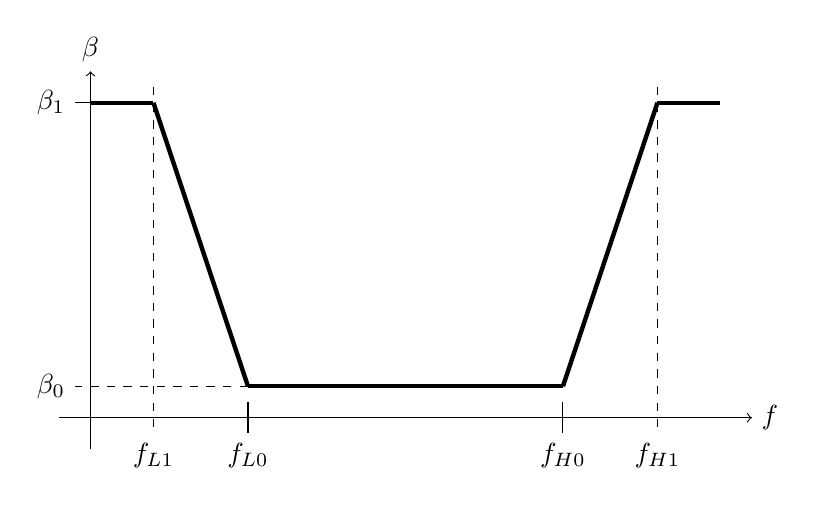
\begin{tikzpicture}[scale=4]
% Parameters
\def\betaone{1}; \def\betazero{0.1};
\def\fzero{0}; \def\fNyq{2};
\def\fLone{0.2}; \def\fLzero{0.5};
\def\fHzero{1.5}; \def\fHone{1.8};

% Axes
\draw[->] (\fzero-0.1,0) -- (\fNyq+0.1,0) node[right]{$f$};
\draw[->] (\fzero,-0.1) -- (\fzero,1.1) node[above]{$\beta$};

% Tick labels
\draw (\fzero+0.05,\betaone) -- (\fzero-0.05,\betaone) node[left]{$\beta_1$};
\draw[dashed] (\fLzero,\betazero) -- (\fzero-0.05,\betazero) node[left]{$\beta_0$};
\draw[dashed] (\fLone,\betaone+0.05) -- (\fLone,-0.05) node[below]{$f_{L1}$};
\draw (\fLzero,0.05) -- (\fLzero,-0.05) node[below]{$f_{L0}$};
\draw (\fHzero,0.05) -- (\fHzero,-0.05) node[below]{$f_{H0}$};
\draw[dashed] (\fHone,\betaone+0.05) -- (\fHone,-0.05) node[below]{$f_{H1}$};

% Plot
\draw[ultra thick] (\fzero,\betaone) -- (\fLone,\betaone);
\draw[ultra thick] (\fLone,\betaone) -- (\fLzero,\betazero);
\draw[ultra thick] (\fLzero,\betazero) -- (\fHzero,\betazero);
\draw[ultra thick] (\fHzero,\betazero) -- (\fHone,\betaone);
\draw[ultra thick] (\fHone,\betaone) -- (\fNyq,\betaone);
\end{tikzpicture}
\caption[Frequency-dependent regularization function for HRTF equalization.]{
Frequency-dependent regularization function of the inverse filters for HRTF equalization.}
\label{fig:A2_SABRE_Toolkit:Farina_Regularization}
\end{figure}

\paragraph*{Diffuse:} For headphones that employ diffuse-field equalization,
we can equalize the HRTFs by the average magnitude spectrum over all directions.
This is computed as the omnidirectional term of the spherical-harmonic decomposition of the HRTF magnitude spectra (in dB),
where the decomposition is computed using the pseudoinverse of $\mathbf{Y}$, given by~\eqnref{eq:YMatrix} for all measurement directions and up to order $L = 4$.
The equalization filter is then computed for the average magnitude spectrum using \eqnref{eq:A2_SABRE_Toolkit:EQ_Filter}.

\paragraph*{Horizontal:} Alternatively, we can compute an average HRTF over all horizontal-plane directions.
The procedure for this is very similar to the diffuse-field equalization, but the average spectrum is computed using only the HRTFs with elevation $|\theta| < 5^\circ$.
The equalization filter is then computed for the average magnitude spectrum using \eqnref{eq:A2_SABRE_Toolkit:EQ_Filter}.

\section{Summary}\label{sec:A2_SABRE_Toolkit:Summary}
The SOFA/ambiX binaural rendering (SABRE) toolkit described here is an open-source collection of MATLAB functions for generating custom binaural decoders.
The toolkit allows a user to construct, using any SOFA-formatted HRTFs, a custom binaural rendering configuration for the ambiX binaural plug-in.
Also implemented in the toolkit are several methods of HRTF interpolation, as well as common HRTF equalization options.
The toolkit is freely available online.\citefooturl{SABREToolkitURL}

\section*{Acknowledgements}
The SABRE toolkit relies on the ambiX ambisonic plug-in suite by \citet{Kronlachner2013,ambiXPlugInURL} and requires head-related transfer functions (HRTFs) stored in the SOFA format \citep{AES69-2015,SOFAMainPageURL}.
Accordingly, the SOFA API for MATLAB is needed to import the HRTF files (available online).\citefooturl{SOFAAPIURL}
The toolkit was originally presented by \citet{TylkaChoueiri2017b} at the 143\textsuperscript{rd} Convention of the Audio Engineering Society. % First referenced in Sec. 2.0, then Sec. 2.7, then Sec. 5.4
%%%% FRACTIONAL OCTAVE SMOOTHING %%%%
\chapter{Log-symmetric fractional-octave smoothing}\label{chap:A3_Smoothing_Weights}
In this appendix, we reproduce a prior publication \citep{Tylka2017} in which we proposed a method for fractional-octave smoothing that, for spectra that are originally symmetric in log-frequency, preserves said symmetry after smoothing.
Unlike an existing method, which requires interpolation of the FFT spectra to a log-frequency scale, the proposed method uses analytically-derived smoothing windows and operates directly in the FFT domain, thereby retaining compatibility with well-established spectral smoothing techniques such as complex smoothing.
In this work, we compared the proposed method to two existing methods by smoothing the magnitude response of an analog band-pass filter (which is symmetric on a log-frequency scale) and subsequently calculating a ``center of mass'' of the smoothed spectra to quantify any loss of symmetry.
The first existing method uses symmetric (on a linear scale) smoothing windows, which exhibit the correct bandwidths but do not span the correct fractional-octave frequency ranges, whereas the second interpolates the spectrum to logarithmically-spaced frequencies and then uses a symmetric fixed-width smoothing window.
As reproduced below, the results of this study showed that the proposed method achieves nearly identical smoothed spectra to the second method, but without the need for interpolation, and that the first method indeed skews the log-symmetry of the original spectra.
Consequently, throughout the present thesis, we employ our proposed method for fractional-octave smoothing where needed (see, in particular, \secref{sec:04_Auditory_Models:Coloration_Metrics:Epk}).

\section{Introduction}\label{sec:A3_Smoothing_Weights:Introduction}
Frequency spectrum smoothing is a standard operation in many fields of audio and acoustics as it reduces the often overwhelming detail of high-resolution spectra to only the relevant information.
Perhaps its most common usage is to make frequency response data suitable for plotting.
However, smoothing is also useful when designing compensation filters for transducer equalization or room response correction, as it both reduces the dynamic range and creates a simplified model of the system to be equalized that, ideally, consists of only the perceptually-relevant information.
In such applications it is important that the peaks (and notches) of the compensation filter align with the corresponding notches (peaks) in the original response, since failure to cancel the notch (peak) may lead to an even worse overall response as a new peak (notch) will have been introduced.
Smoothing methods must therefore be employed carefully so that prominent features of the frequency response such as peaks and notches are not unintentionally shifted during the smoothing process.

One application of spectral smoothing is in the design of headphone equalization (EQ) filters, wherein the headphone transfer function (which describes the transmission of sound from the headphones to the listener's ear drums) is first smoothed and then either inverted and used directly as the EQ filter, or used to define a regularization function that improves the conditioning of the inversion operation and mitigates excessive boosting in the EQ filter \citep{ScharerLindau2009}.
Spectral smoothing is also used in binaural audio to reduce the complexity of the head-related transfer function (HRTF), which describes the transmission of sound from a point in space to a listener's ear drums.
As a listener's HRTF often contains more detailed spectral information than is perceptually relevant, measured HRTFs can be smoothed to a certain degree without loss of localization accuracy or externalization \citep{XieZhang2010, Hassager2014}.
This enables a simplified model of a listener's HRTF to be used to generate perceptually-accurate personalized binaural audio \citep{Rasumow2014}.

In these and other applications, it is often desired to obtain an impulse response after smoothing that retains the perceptually-relevant temporal features of the original impulse response.
To this end, \citet{HatziantoniouMourjopoulos2000} proposed ``complex smoothing,'' which extends the procedure of fractional-octave smoothing to complex-valued transfer functions (as opposed to the squared magnitude response used in traditional power-spectrum smoothing) and enables the calculation of a ``smoothed'' impulse response.
More recently, \citet{Volk2011} proposed a method that uses complex-valued smoothing windows (corresponding to exponentially-decaying time windows applied to the impulse response) to better approximate the temporal and spectral smoothing inherent to the human auditory system.
Also, as an alternative to complex smoothing, \citet{Bank2013} presented a method of modeling transfer functions by a finite number of parallel second-order filters (whose poles are typically logarithmically-spaced in frequency), and showed that this method achieves a frequency resolution similar to that of fractional-octave smoothing.
Due to this current interest in obtaining equivalent time-domain responses after smoothing, any new spectral smoothing method should either retain compatibility with complex smoothing or prescribe an alternative method of obtaining the smoothed impulse response.

% Review of previous work focusing on the remaining problems (questions or deficiencies) the present paper claims to contribute to solving
\subsection{Previous work and remaining problems}
Fractional-octave smoothing is a special case of spectral smoothing in which the bandwidth of the smoothing window is a constant percentage of the center frequency.
Consequently, to smooth frequency spectra obtained via the fast Fourier transform (FFT) of a discrete-time signal, wherein the spectral data points are uniformly spaced in frequency, the fractional-octave smoothing window must vary with frequency.
\citet{HatziantoniouMourjopoulos2000} presented a method and general framework for smoothing FFT-based frequency spectra to an arbitrary frequency resolution.
However, this method prescribes smoothing windows that are symmetric on a linear frequency scale (and therefore do not span the correct fractional-octave bands), which consequently introduces an error, as is shown in the present work.
\citet{Lipshitz1985} prescribe interpolating the FFT spectrum to a logarithmic frequency (log-frequency) scale, so that a fixed-width moving-average filter may be employed.
As is shown in the present work, this approach is able to preserve the log-symmetry of raw spectra but requires leaving the FFT domain via interpolation, incurring a computational cost and necessarily introducing errors.

% A statement of the paper's main question(s) and goal(s), followed by a succinct description of the general method and approach to be described in the paper
\subsection{Objectives and approach}
The goal of this work is to derive a fractional-octave smoothing method that preserves the log-symmetry of the original spectrum.
Ideally, such a method should also operate directly on FFT-based frequency spectra, without the need to interpolate to a non-uniform frequency scale, and should be compatible with complex smoothing.
Additionally, we evaluate the ability of existing fractional-octave smoothing methods to preserve log-frequency symmetry seen in the original spectrum.
To evaluate the methods considered in this work, we apply each method to the magnitude response of an analog band-pass filter, which is symmetric on a log-frequency scale.
Any loss of symmetry is examined in terms of a ``center of mass'' of the smoothed spectrum.

% A brief section by section description of the structure of the paper
In \secref{sec:A3_Smoothing_Weights:Smoothing_Methods} we present the framework for fractional-octave smoothing, followed by a brief review of the symmetric-window method in \secref{sec:A3_Smoothing_Weights:Smoothing_Methods:Hatziantoniou_Method} and the log-frequency interpolation method in \secref{sec:A3_Smoothing_Weights:Smoothing_Methods:Lipshitz_Method}.
We then propose an alternative method in \secref{sec:A3_Smoothing_Weights:Smoothing_Methods:Proposed_Method}, perform a comparative analysis of the three methods in \secref{sec:A3_Smoothing_Weights:Analysis}, and conclude.

\section{Smoothing methods}\label{sec:A3_Smoothing_Weights:Smoothing_Methods}
In general, spectral smoothing may be applied to any function of frequency.
Here, we restrict our discussion to raw (i.e., not smoothed) frequency spectra whose data points are specified at uniformly-spaced frequencies on a linear scale, such as those obtained through an FFT.
Furthermore, in the applications of spectral smoothing mentioned in the introduction, the spectra to be smoothed are typically frequency or magnitude responses of acoustic transfer functions, rather than Fourier transforms or power spectra of time-domain signals.\footnote{This distinction becomes necessary when discussing interpolation to a log-frequency scale.
For example, for power spectra of time-domain signals, conversion from a linear frequency scale to a log-frequency scale should also involve a change of units of the vertical axis, such that the values that are plotted on a linear frequency scale represent power per unit linear frequency, whereas those plotted on a log-frequency scale represent power per unit log-frequency.
Through this conversion, a pink-noise power spectrum plotted over linear frequency would exhibit the usual $-3$~dB/octave slope, while on a log-scale, the spectrum would appear flat.
Consequently, on either frequency scale, integrating the power spectrum over a given frequency band gives the total power in that band.
However, for frequency (or magnitude) responses of transfer functions, the values that are plotted are gains for specific frequencies, regardless of the distribution of those frequency points.
Consequently, interpolation of a frequency response to a log-frequency scale should involve only a ``resampling'' of the response to logarithmically-spaced frequencies; it should not involve a change of units.} Consequently, we further restrict our discussion to the smoothing of frequency or magnitude responses of transfer functions.

Consider a raw, possibly complex-valued frequency spectrum of length $N$ denoted by $X[k]$, where $k$ is the discrete frequency index.
The smoothed spectrum is given by
\begin{equation}\label{eq:A3_Smoothing_Weights:SmoothingSummation}
X_\textrm{s}[k] = \sum_{k' = 0}^{N - 1} W[k, k'] X[k']
\end{equation}
for all integers $k,k' \in [0, N - 1]$, where, for a given value of $k$, $W[k, k']$ denotes the $k^{\textrm{th}}$ sequence of non-negative weights used to smooth the raw spectrum \citep{HatziantoniouMourjopoulos2000}.
These weights are normalized such that, for all $k \in [0, N - 1]$,
\begin{equation}\label{eq:A3_Smoothing_Weights:WeightNorm}
\sum_{k' = 0}^{N - 1} W[k, k'] = 1.
\end{equation}

The smoothing operation defined by \eqnref{eq:A3_Smoothing_Weights:SmoothingSummation} can be thought of as a frequency-domain convolution with a frequency-dependent kernel, $W[k, k']$.
In the case of a frequency-invariant smoothing window (e.g., a fixed-width moving-average filter), we can instead define a single weight sequence $W[k - k'] = W[k, k']$, and \eqnref{eq:A3_Smoothing_Weights:SmoothingSummation} takes the standard form of convolution.

To compute the smoothed spectrum at a given frequency $f = k F_s / N$, where $F_s$ is the sampling rate, the (exact) lower and upper cutoff frequencies of the weighting function are given by
\begin{equation}\label{eq:A3_Smoothing_Weights:cutoffs}
    \begin{array}{ll}
    f_L &= f \cdot 2^{-\Delta/2},\\[8pt]
    f_U &= f \cdot 2^{+\Delta/2},
    \end{array}
\end{equation}
respectively \citep{HatziantoniouMourjopoulos2000}, where $\Delta$ is the smoothing bandwidth in octaves.
Consequently, the ratio, $Q$, of the center frequency to the bandwidth is a constant, and its reciprocal is given by
\begin{equation}\label{eq:A3_Smoothing_Weights:QFactor}
\frac{1}{Q} = \frac{f_U-f_L}{f} = 2 \sinh \left( \frac{\Delta \log (2)}{2} \right).
\end{equation}

%%%% Hatziantoniou's Method %%%%
\subsection{Method 1: symmetric weights} \label{sec:A3_Smoothing_Weights:Smoothing_Methods:Hatziantoniou_Method}
In the method presented by~\citet{HatziantoniouMourjopoulos2000}, the smoothed spectrum is computed using~\eqnref{eq:A3_Smoothing_Weights:SmoothingSummation}, where the weighting function is derived by first defining the half-length of the $k^{\textrm{th}}$ weight sequence as
\begin{equation}\label{eq:A3_Smoothing_Weights:HatzHalfWidth}
m[k] = \left\lfloor \frac{1}{2}\frac{k}{Q} \right\rfloor,
\end{equation}
where $\lfloor \cdot \rfloor$ denotes rounding down to the nearest integer.
The weighting function for a rectangular window is then given by
\begin{equation}\label{eq:A3_Smoothing_Weights:HatzWeights}
W_{\textrm{R}}[k, k'] = \left\{
    \begin{array}{cl}
	\displaystyle \frac{1}{2 m[k] + 1} & \textrm{for } \left| k - k' \right| \leq m[k],\\[8pt]
	0 & \textrm{for } \left| k - k' \right| > m[k].
    \end{array}\right.
\end{equation}
From this definition we see that each weight sequence is a rectangular window with $2 m[k] + 1$ non-zero values centered around $k = k'$.
This is in conflict with~\eqnref{eq:A3_Smoothing_Weights:cutoffs}, as the upper cutoff frequency should be further from the center than the lower cutoff, but instead the two ends of the weight sequence are equidistant to the center.
As we will show in~\secref{sec:A3_Smoothing_Weights:Analysis}, this error becomes significant for large smoothing bandwidths.

%%%% Lipshitz' Method %%%%
\subsection{Method 2: interpolation to logarithmic scale} \label{sec:A3_Smoothing_Weights:Smoothing_Methods:Lipshitz_Method}
In the method proposed by~\citet{Lipshitz1985}, the raw spectrum is first interpolated to a logarithmic frequency scale, at which point a fixed-width moving-average filter is applied.
The authors suggest interpolating to $N/2$ logarithmically-spaced frequencies, which we denote $\kappa[\ell]$, given by
\begin{equation}
\kappa[\ell] = \left( \frac{N}{2} \right)^\frac{\ell}{N/2-1},
\end{equation}
such that $1 \leq \kappa[\ell] \leq N/2$ for all integers $\ell \in [0, N/2 - 1]$.
The interval in octaves between any two adjacent frequencies is a constant, given by
\begin{equation}
\beta = \log_2 \frac{\kappa[\ell + 1]}{\kappa[\ell]} = \frac{1}{N/2-1} \log_2 \frac{N}{2},
\end{equation}
and, as we did for method 1, we define the weight-sequence half-length, $\mu$, as
\begin{equation}
\mu = \left\lfloor \frac{\Delta/2}{\beta} \right\rfloor,
\end{equation}
which is also constant.

To perform the interpolation,~\citet{Lipshitz1985} suggest a 4-point polynomial (i.e., cubic) interpolation, but, in general, any interpolation scheme (e.g., linear, spline, etc.) may be employed.
Here, we use linear interpolation, such that the interpolated raw spectrum, $\hat{X}$, which is now a function of the log-frequency index $\ell$, is given by
\begin{equation}\label{eq:A3_Smoothing_Weights:LogInterpolate}
\hat{X}[\ell] = X[k_1] + \left( X[k_2] - X[k_1] \right) \frac{\kappa[\ell] - k_1}{k_2 - k_1},
\end{equation}
where $k_1 = \big\lfloor \kappa[\ell] \big\rfloor$ and $k_2 = k_1 + 1$.

The smoothed spectrum, $\hat{X_\textrm{s}}$, is also a function of $\ell$ and is given by
\begin{equation}
\hat{X_\textrm{s}}[\ell] = \sum_{\ell' = 0}^{N/2 - 1} \hat{W}[\ell - \ell'] \hat{X}[\ell'],
\end{equation}
where $\hat{W}$ is the weighting function.
For a rectangular window, $\hat{W}$ is given by
\begin{equation}
\hat{W}_{\textrm{R}}[\ell - \ell'] = \left\{
    \begin{array}{cl}
	\displaystyle \frac{1}{2 \mu + 1} & \textrm{for } \left| \ell - \ell' \right| \leq \mu,\\[8pt]
	0 & \textrm{for } \left| \ell - \ell' \right| > \mu.
    \end{array}\right.
\end{equation}
The smoothed spectrum is then interpolated back to a linear frequency scale by
\begin{equation}
X_\textrm{s}[k] = \hat{X_\textrm{s}}[\ell_1] + \left( \hat{X_\textrm{s}}[\ell_2] - \hat{X_\textrm{s}}[\ell_1] \right) \frac{k - \kappa[\ell_1]}{\kappa[\ell_2] - \kappa[\ell_1]},
\end{equation}
where $\ell_1 = \left\lfloor (N/2 - 1) \log_{N/2} (k) \right\rfloor$ and $\ell_2 = \ell_1 + 1$.

%%%% Proposed Method %%%%
\subsection{Method 3: logarithmically-compensated weights} \label{sec:A3_Smoothing_Weights:Smoothing_Methods:Proposed_Method}
Consider a window $w(\phi)$ that is a function of the continuous variable $\phi$ (we will see later that $\phi$ is related to frequency).
Let $w$ be an even function of $\phi$ whose total integral is unity, i.e.,
\begin{equation}\label{eq:A3_Smoothing_Weights:WindowNorm}
\int_{-\infty}^{\infty} w(\phi) d\phi = 1.
\end{equation}

For example, given a smoothing bandwidth of $\Delta$ octaves, the normalized rectangular window is given by
\begin{equation}\label{eq:A3_Smoothing_Weights:RectangularWindowLogf}
w_\textrm{R}(\phi) = \left\{
    \begin{array}{cl}
	1/\Delta & \textrm{for } |\phi| \leq \Delta/2,\\[8pt]
	0 & \textrm{for } |\phi| > \Delta/2.
    \end{array}\right.
\end{equation}

For a given center-frequency index, $k$, we compute the weighting function by successively integrating adjacent slices of the window function, i.e.,
\begin{equation}\label{eq:A3_Smoothing_Weights:WeightsIntegral}
W[k, k'] = \int_{\Phi[k, k' - 0.5]}^{\Phi[k, k' + 0.5]} w(\phi) d\phi
\end{equation}
for all integers $k,k' \in [0, N - 1]$, where $\phi$ represents log-frequency in octaves relative to $k$, i.e., $\log_2(k'/k)$, and the limits of integration are given by
\begin{equation}\label{eq:A3_Smoothing_Weights:WeightsIntegralLimits}
\Phi[k, k' \pm 0.5] = \log_2 \left( \frac{k' \pm 0.5}{k} \right).
\end{equation}
As for method 1, the smoothed spectrum is then computed using~\eqnref{eq:A3_Smoothing_Weights:SmoothingSummation} but with this new weighting function.
Due to the normalization of the window function imposed in~\eqnref{eq:A3_Smoothing_Weights:WindowNorm}, each resulting weight sequence is also normalized and satisfies~\eqnref{eq:A3_Smoothing_Weights:WeightNorm}.

%% Example %%
%\begin{example*}
\paragraph*{Example:} To illustrate the difference between the calculated weights and the window function, consider the weight sequence needed to compute the value of the smoothed spectrum at $k = 10$, for 1-octave smoothing.
The window function is given by \eqnref{eq:A3_Smoothing_Weights:RectangularWindowLogf}, and the weights will be non-zero for, at most, $\lfloor k \cdot 2^{-\Delta/2} \rfloor \leq k' \leq \lceil k \cdot 2^{+\Delta/2} \rceil$, i.e., $k' \in [7, 15]$, where $\lceil \cdot \rceil$ denotes rounding up to the nearest integer and the bounds of the inequalities are obtained by substituting $k$ for $f$ in~\eqnref{eq:A3_Smoothing_Weights:cutoffs}.
However, integrating the window function for all slices reveals that $W[10,15] = 0$, since that integral begins at $\log_2 (14.5/10)$ but the window function already dropped to zero at $\phi \approx \log_2 (14.142/10)$.

\begin{figure}[t]
    \centering
    \includegraphics[width=0.6\columnwidth]{a3_smoothing_weights/figures/RectangularWeightsExample.eps}
    \caption[Calculated smoothing weights for a rectangular window function.]{
    Calculated weighting function $W[k,k']$ for methods 1 (symmetric weights -- empty circles) and 3 (log-compensated weights -- filled circles) for a rectangular window function $w(\phi)$ (solid curve).
In this example, $k = 10$ and $\Delta = 1$~octave.
Dashed vertical lines (and ticks on the top axis) indicate the limits of integration, $\Phi[10, k' \pm 0.5]$, given by \eqnref{eq:A3_Smoothing_Weights:WeightsIntegralLimits}.}
    \label{fig:A3_Smoothing_Weights:RectangularWeightsExample}
\end{figure}

The calculated non-zero weights are shown as filled circles in \figref{fig:A3_Smoothing_Weights:RectangularWeightsExample} along with the window function, both as functions of $\phi$.
From this plot, we observe two features of the weight sequence.
First, the end points take into account the extent to which the window function occupies the corresponding frequency interval, whereas simply evaluating the window function at each $k'$ would only ever give either 0 or $1/\Delta$.
Second, the intermediate points exhibit a frequency-dependent trend similar to that of a pink-noise power spectrum.
Indeed, this sequence is derived to assign equal weight per unit log-frequency (e.g., octave), so although the width of each frequency interval is constant, the ratio between the upper and lower edges of the interval decreases with increasing frequency, so the weight must also decrease.

For comparison, the weights for method 1 are also shown in \figref{fig:A3_Smoothing_Weights:RectangularWeightsExample} as empty circles that remain constant ($W[k,k'] = 1/7$) for $| k - k' | \leq m[k] = 3$ and zero otherwise.
%\end{example*}

\section{Analysis}\label{sec:A3_Smoothing_Weights:Analysis}
To examine how each smoothing method affects log-frequency symmetry, we apply each method to the magnitude response of an analog band-pass filter whose frequency response is given by
\begin{equation}
H(i \omega) = \frac{\frac{i\omega}{\omega_0}/Q}{1 + \frac{i\omega}{\omega_0}/Q + (\frac{i\omega}{\omega_0})^2}.
\end{equation}
In this analysis, we choose a $1/6^{\textrm{th}}$-octave band-pass filter ($Q \approx 8.65$ from \eqnref{eq:A3_Smoothing_Weights:QFactor}) with a center frequency of $f_0 = \omega_0/(2\pi) = 5000$~Hz, and sample the frequency response above at $N = 4096$ points, with a frequency resolution of $\approx24$~Hz (i.e., $F_s = 100,000$~samples/s).
The raw spectrum is then given by $X[k] = \left| H(2 \pi i k F_s / N) \right|^2$.

To quantify any skewing of log-frequency symmetry, we compare the center frequency, $f_0$, of the band-pass filter to the ``center of mass,'' $f_c$, of each smoothed spectrum.%
\footnote{There is a subtle but important distinction between the center of mass of a magnitude response (as defined here) and that of the power spectrum of a signal (also known as the ``spectral centroid'').
For a magnitude response, we can arbitrarily choose frequencies at which to sample the response, although doing so may change the result.
A signal's power spectrum, however, cannot be resampled arbitrarily, as its data points represent power per unit frequency, and therefore its center of mass is unambiguously defined.} We define $f_c$ in coordinates of log-frequency such that, for our chosen raw spectrum (which is symmetric in log-frequency), the result is equal to $f_0$.
This center of mass is given by
\begin{equation}
f_c = \exp \left( {\frac{\displaystyle \sum_{\ell = \ell_0 - \lceil 2/\beta \rceil}^{\ell_0 + \lceil 2/\beta \rceil} \log \left( \frac{\kappa[\ell] F_s}{N} \right) \hat{X_\textrm{s}} [\ell]}{\displaystyle \sum_{\ell = \ell_0 - \lceil 2/\beta \rceil}^{\ell_0 + \lceil 2/\beta \rceil} \hat{X_\textrm{s}} [\ell]}} \right),
\end{equation}
where $\hat{X_\textrm{s}}$ is the smoothed spectrum interpolated to a log-frequency scale, obtained using~\eqnref{eq:A3_Smoothing_Weights:LogInterpolate} with $X_\textrm{s}$ in place of $X$, and $\ell_0$ is the log-frequency index corresponding to the center frequency $f_0$ of the band-pass filter, given by
\begin{equation*}
\ell_0 = \textrm{Round} \left[ \left( \frac{N}{2} - 1 \right) \log_{N/2} \left( \frac{N f_0}{F_s} \right) \right].
\end{equation*}
The limits of the summation, $\ell_0 \pm \lceil 2/\beta \rceil$, indicate averaging over two octaves above and two below $f_0$.
The error in the center of mass is then given in percent by
\begin{equation}
\epsilon = 100 \times \frac{f_c - f_0}{f_0}.
\end{equation}

%%%% RESULTS %%%%
\subsection{Results} \label{sec:A3_Smoothing_Weights:Results}
The differences between the three smoothing methods can be seen qualitatively in \figref{fig:A3_Smoothing_Weights:SmoothedBPFExample}, which shows the smoothed spectra produced by each of these methods using rectangular windows and 1-octave smoothing.
We see from this plot that not only is method 1 unable to preserve the log-frequency symmetry observed in the raw spectrum, but also the smoothed spectrum for method 1 appears shifted to the right (i.e., blue-shifted) relative to those of methods 2 and 3 and to the original spectrum.

\begin{figure}[t]
    \centering
    \includegraphics[width=0.6\columnwidth]{a3_smoothing_weights/figures/SmoothedBPFExample.eps}
    \caption[Original and smoothed magnitude responses of a band-pass filter.]{
    Original and 1-octave-smoothed spectra for the magnitude response of an analog band-pass filter.
Method 1 refers to the symmetric weights method; 2 to interpolation to a log-frequency scale; and 3 to log-compensated weights.
The smoothed spectra produced by methods 2 and 3 are nearly identical, so both are represented by the black curve.
The bottom axis shows frequency relative to the center frequency, $f_0$, of the band-pass filter, while the top axis shows frequency in kHz for $f_0 = 5$~kHz.}
    \label{fig:A3_Smoothing_Weights:SmoothedBPFExample}
\end{figure}

The errors in the center of mass are plotted in \figref{fig:A3_Smoothing_Weights:CenterOfMassAnalysis} for each smoothing method and for a range of smoothing bandwidths.
We see from this plot that the center of mass of the smoothed spectrum generated by method 1 increases in frequency as smoothing bandwidth increases.
For small smoothing bandwidths ($\Delta < 1/3$~octave), this error is quite small ($< 1\%$), but becomes large ($\sim 10\%$) for large smoothing bandwidths.

\begin{figure}[t]
    \centering
    \includegraphics[width=0.6\columnwidth]{a3_smoothing_weights/figures/CenterOfMassAnalysis.eps}
    \caption[Error in the center of mass for different smoothing bandwidths.]{
    Error, $\epsilon$, in the center of mass for different smoothing bandwidths, $\Delta$.
Method 1 refers to the symmetric weights method (denoted by filled circles); 2 to interpolation to a log-frequency scale (triangles); and 3 to log-compensated weights (squares).
Plot markers for methods 2 and 3 are alternated for legibility.}
    \label{fig:A3_Smoothing_Weights:CenterOfMassAnalysis}
\end{figure}

Contrary to the center of mass, the maximum of the smoothed spectrum for method 1 appears shifted to the \textit{left} relative to that of the original spectrum (see \figref{fig:A3_Smoothing_Weights:SmoothedBPFExample}).
To further explore this phenomenon, we apply methods 1 and 3 to smooth a unit impulse located at $f_0$, as shown in \figref{fig:A3_Smoothing_Weights:SmoothingImpulseResponse}.
From this plot we see that the maximum of the smoothed spectrum for method 1 occurs at a significantly lower frequency than $f_0$, although the precise location of the maximum will depend on the raw spectrum (e.g., the width of the raw peak), the smoothing window, and the smoothing bandwidth.

\begin{figure}[t]
    \centering
    \includegraphics[width=0.6\columnwidth]{a3_smoothing_weights/figures/SmoothingImpulseResponse.eps}
    \caption[Original and smoothed spectra for a unit impulse.]{
    Original and 1-octave-smoothed spectra for a unit impulse located at $f_0$, computed for methods 1 (symmetric weights) and 3 (log-compensated weights).
The smoothed spectra are multiplied by a factor of 100 for legibility.
The bottom axis shows frequency relative to $f_0$, while the top axis shows frequency in kHz for $f_0 = 5$~kHz.}
    \label{fig:A3_Smoothing_Weights:SmoothingImpulseResponse}
\end{figure}

The reason for this shift can be understood in terms of the contribution of the raw spectrum's maximum to each smoothed value.
From \eqnreftwo{eq:A3_Smoothing_Weights:HatzHalfWidth}{eq:A3_Smoothing_Weights:HatzWeights}, as frequency $k$ increases, the width of the smoothing window increases and, due to the normalization of the weights, its amplitude decreases.
Consequently, the contribution of the raw spectrum's maximum to the smoothed value decreases as frequency increases, yielding, in this case, a steadily decreasing smoothed spectrum.

Method 3, on the other hand, creates a uniform spectrum that is symmetric about $f_0$, but has no single maximum.
However, it can be verified that for other smoothing windows (e.g., Hanning), the peak appears at $f_0$.

\section{Conclusions}\label{sec:A3_Smoothing_Weights:Conclusions}
In this work we explored the ability (or lack thereof) of fractional-octave smoothing methods to preserve the log-frequency symmetry of frequency spectra.
Specifically, we examined two existing methods of smoothing, the first of which uses a symmetric (on a linear frequency scale) window of the correct bandwidth, but whose cutoff frequencies are not equidistant from the center frequency when viewed on a log-frequency scale, and therefore do not correspond to the \textit{correct} fractional-octave band.
The second method requires that the raw spectrum first be interpolated to a log-frequency scale, a process that necessarily introduces errors, but simplifies the fractional-octave smoothing procedure to a moving-average operation with a symmetric window that corresponds well with the correct fractional-octave band.
We proposed a third smoothing method that is able to accurately replicate the smoothed spectrum of the second method but without the need for interpolation.
This method is fully compatible with other FFT-based smoothing techniques such as complex smoothing (see \citet{HatziantoniouMourjopoulos2000}) and can be employed with any smoothing window (e.g., Hanning window, band-pass filter, etc.), provided the window can be specified as an integrable function of log-frequency.

We performed a numerical analysis of the ``center of mass'' of the smoothed spectra produced by each method given the magnitude response of an analog band-pass filter (which is symmetric on a log-frequency scale) as the raw spectrum.
This analysis revealed that only the first method is unable to preserve the log-symmetry of the raw spectrum, as it shifts the center of mass upwards in frequency, resulting in a ``blue-shifted'' smoothed spectrum.
It is worth noting that this error is quite small for small smoothing bandwidths (e.g., the center of mass shifts by $< 1 \%$ of the center frequency for $1/3$-octave smoothing) and therefore may be tolerable in some applications.
We also smoothed a unit impulse with the first and third methods to explore how the maximum may shift after smoothing.
Results showed that only the first method shifts the maximum downwards in frequency, although we expect this phenomenon to be less significant for smaller smoothing bandwidths.

Regarding the computational cost of the proposed method, it is relevant to note that, for many smoothing windows, the definite integral of the window (see \eqnref{eq:A3_Smoothing_Weights:WeightsIntegral}) can be evaluated analytically, making the calculation of each weight sequence computationally inexpensive.
Furthermore, for all smoothing windows, the weighting function can be precomputed and stored in a matrix, recasting the smoothing operation as a matrix multiplication whose computational expense would be invariant with smoothing method, window, and bandwidth.

Future work should include an exploration of the equivalent time-domain implementation of the proposed method, wherein smoothing is expressed as multiplication of the input impulse response with frequency-dependent windows \citep{HatziantoniouMourjopoulos2000} and an investigation into the perceptual differences, if any, between the first and third methods for various smoothing bandwidths and in various applications (e.g., digital room correction, headphone equalization, etc.).

\section*{Acknowledgements}
This work was originally published by \citet{Tylka2017} in \textit{The Journal of the Audio Engineering Society}.
The present author wishes to thank R.~Sridhar for fruitful discussions during this work and the anonymous reviewers for their feedback. % First referenced in Sec. 4.2.2
%%%% HRTF MEASUREMENTS %%%%
\chapter{Head-related transfer function measurements}\label{chap:A4_HRTF_Measurements}
In this appendix, we describe the measurement and data processing procedures employed in the present thesis (see \chapref{chap:05_Proposed_Models}) to capture the head-related transfer functions (HRTFs) of human subjects.
These procedures were developed and published as part of an on-going project to generate a database of HRTF and morphological measurements of humans and mannequins \citep{Sridhar2017}.
Since only a few such databases are freely available, this database was created to facilitate the development of data-driven HRTF estimation techniques, which require large datasets of measured HRTFs and morphological data.
In the original paper, the head scanning and corresponding processing procedures are also described, but we omit these details here.

\section{Introduction}\label{sec:A4_HRTF_Measurements:Introduction}
Head-related transfer functions (HRTFs) of an individual describe the idiosyncratic filtering of incident acoustic waves by the individual's morphology and are widely used in synthesizing binaural signals for spatial audio reproduction.
The most accurate way to acquire HRTFs is via acoustical measurements in an anechoic chamber \citep[chapter 2]{Xie2013}.

% We need individually measured HRTFs for our research
Many publicly available databases exist that include measured HRTFs for many human subjects and mannequins \citep[for example]{SOFAHRTFDatabasesURL}.
However, these databases are not perfect; many of the measured head-related impulse responses (HRIRs) from both the RIEC \citep{Watanabe2014,RIECHRTFDatabaseURL} and CIPIC \citep{Algazi2001} databases have undesirable pre-responses prior to the main impulses, which may make the data unreliable for use without sufficient post-processing.
Furthermore, it is not guaranteed that, for any given individual, a suitable set of HRTFs will be found in any existing database.
Consequently, in order to provide the highest-spatial-fidelity in listening tests and minimize errors in HRTFs as a source of error in the test results, individual HRTF measurements should be made for every listening test subject.

% Also, putting together a database helps the community
Since individual measurement of HRTFs is commercially infeasible, alternative techniques for estimating HRTFs have been proposed, many of which are summarized by \citet{Xie2013}.
Most techniques require morphological data that includes either measurements of specific anthropometric features \citep{Bilinski2014} or complete 3D scans of the individual's morphology \citep{Gumerov2010}.
Data-driven techniques additionally require corresponding measured HRTFs of a large number of individuals.
These HRTFs typically serve as benchmarks for validating different techniques either objectively or via subjective listening tests, and also serve as training data for data-driven techniques.
For example, a recent data-driven technique to compute HRTFs directly from head scan point clouds requires measured HRTFs and 3D head scans of many individuals as training data \citep{SridharChoueiri2017}.
Consequently, gathering new HRTF and 3D morphological scan data enables others to develop and improve such HRTF estimation techniques.

Recognizing the growing need for measured HRTF and 3D morphological data, we have begun an on-going project to measure HRTFs and 3D scans of humans and mannequins, which we compile into a publicly available database.
In \secref{sec:A4_HRTF_Measurements:Measurement_Procedure}, we present details of the measurement procedures.
In \secref{sec:A4_HRTF_Measurements:Data_Processing}, we describe the signal processing performed on the measured data.
We visualize a sample of the data in \secref{sec:A4_HRTF_Measurements:Data_Visualization} and summarize our work in \secref{sec:A4_HRTF_Measurements:Summary}.

\section{Measurement procedure}\label{sec:A4_HRTF_Measurements:Measurement_Procedure}
We conduct acoustical measurements in a $3.6 \times 2.35 \times 2.55$~m ($l \times w \times h$) anechoic chamber with 8-inch deep (equal to $1/4$ wavelength at $\sim425$~Hz) anechoic foam wedges.
In the chamber, we place a circular arc which stands vertically and is aligned to be concentric with the ``origin'' of the chamber (i.e., where the center of the subject's head is ultimately placed). 
We attach to the arc eight loudspeakers (Genelec 8030A), which are equally-spaced (in $15^\circ$ increments) between $-30^\circ$ and $75^\circ$ elevation, and we include a ninth loudspeaker mounted on a separate stand at $-57^\circ$ elevation.\footnote{Here, we use the same spherical coordinate system as that defined in \citet{AES69-2015}.}
Specifically, we align the high-frequency drivers of the loudspeakers with these elevations such that the distance from each high-frequency driver to the origin is approximately $0.76 \pm 0.005$~m.
We also place, directly below the origin, a custom-built chair that is affixed to a computer-controlled turntable (Outline ET250-3D), whose axis of rotation passes through the origin of the chamber.
The chair, which is designed to have a minimal effect on incident acoustic waves,
consists of a drum-throne seat with backrest and a thin ``headrest'' structure that provides a reference for positioning the subject's head,
in order to minimize head movements during measurements.
An image of the setup is shown in \figref{fig:HRTF_setup}.

\begin{figure}[t]
\begin{center}
\includegraphics[width = 0.7\textwidth]{a4_HRTF_measurements/figures/HRTF_setup.png}
\caption{Setup used to make HRTF measurements.}.
\label{fig:HRTF_setup}
\end{center}
\end{figure}

Prior to making measurements, we calibrate and equalize the binaural microphones (Theoretica Applied Physics BACCH-BM Pro).
We first adjust, for each channel, the microphone gain (using a B\&K Type 4231 calibrator and DP-0978 adapter) such that a 94~dBSPL (rms) sine tone produces a $-11$~dBFS (peak) signal.
We then place the microphones at the origin of the chamber, facing the arc and parallel to the horizontal plane, in order to measure a set of nine ``reference'' impulse responses (RIRs), one for each elevation. % Joe: What about mic directivity? Rahul: Maybe we don't need to address this here. Perhaps in an auxiliary document?
For these measurements, we remove the seat cushion, backrest, and headrest, and then cover the remaining metal structure of the chair with anechoic foam wedges in order to minimize the acoustical influence of the chair-structure on the measurements.

We measure the RIRs by sending to the loudspeakers a series of partially-overlapping exponential sine sweeps \citep{Majdak2007} (generated in Plogue Bidule) and recording the resulting signals with the microphones. % Joe: Include speaker frequency responses? Rahul: I don't think this is necessary here. Maybe in an auxiliary document.
The delay between each successive sweep is 200~ms, yielding distinct impulse responses of up to 200~ms in duration.
All measurements are conducted at a sampling rate of 96~kHz and the sweep signals are generated with a nominal frequency range of 20~Hz to 48~kHz, a duration of 500~ms, and an amplitude (at 1~kHz) of 70~dBSPL (rms).
The measured signal-to-noise ratio is approximately 38.5~dB for each microphone.
The RIRs are used to equalize the transfer functions of each loudspeaker-microphone pair, as described in \secref{sec:A4_HRTF_Measurements:Data_Processing}.

For each subject, we measure binaural impulse responses (BIRs) for 648 directions: all nine loudspeaker elevations for each of 72 azimuths (equally spaced between $0^\circ$ and $355^\circ$).
We seat the subject on the chair such that the center of the subject's head coincides with the origin.
We then place the binaural microphones at the entrances to the subject's blocked ear canals and measure BIRs using the same multiple exponential sine sweeps described above.
The subject is rotated in $5^{\circ}$ increments and the sweeps are repeated until the measurements are complete.
In total, these measurements (including rotation time) takes $\sim11$ minutes.

\section{Data processing}\label{sec:A4_HRTF_Measurements:Data_Processing}
The head-related impulse responses (HRIRs) are obtained by equalizing, for each subject and for each loudspeaker-microphone pair, the measured binaural impulse responses (BIRs) by the corresponding reference impulse responses (RIRs).
We first apply a 42 ms rectangular window to all of the raw BIRs and RIRs.
We then generate inverse filters for the RIRs using frequency-dependent regularization,
such that the transfer function of the inverse filter is given by \eqnref{eq:A2_SABRE_Toolkit:EQ_Filter}, where now $H$ is the transfer function of a measured RIR.
The regularization function is defined by a set of parameters, which are defined graphically in \figref{fig:A2_SABRE_Toolkit:Farina_Regularization}, and whose default values are given by
\begin{equation*}
\begin{array}{l l l}
\beta_0 = 0, &f_{L0} = 100~\text{Hz}, &f_{H0} = 30~\text{kHz}, \\
\beta_1 = 10^{-3}, &f_{L1} = 50~\text{Hz}, &f_{H1} = 32~\text{kHz}.
\end{array}
\end{equation*}
These values were found to sufficiently limit any pre-responses in the equalized HRIRs (see \secref{sec:A4_HRTF_Measurements:Data_Visualization}), while retaining a wide usable bandwidth. 
Finally, we convolve the BIRs with these inverse filters and apply a Tukey window to generate HRIRs that have an approximate duration of 10 ms.
The BIRs, RIRs, and HRIRs are all included in the database as separate SOFA (spatially-oriented format for acoustics) files \citep{AES69-2015}.

\section{Data visualization}\label{sec:A4_HRTF_Measurements:Data_Visualization}
To verify that the our measured HRTFs are free of artifacts (e.g., pre-responses prior to the main impulses), we generate a surface plot of ITD estimated from measured HRTFs using a thresholding approach (see, for example, \citet{KatzNoisternig2014}) with a 20\% threshold.
\Figref{fig:Sample_ITD_surface} shows this surface plot for one of the subjects in our database.
This plot shows a plausible ITD surface, as it is generally smooth and free of discontinuities, suggesting that the data are free of significant artifacts, noise, or any other errors.

\begin{figure}[t]
\begin{center}
\includegraphics[width = 0.7\textwidth]{a4_HRTF_measurements/figures/Sample_ITD_surface.pdf}
\caption[Surface plot of typical interaural time differences.]{Surface plot of ITD in $\mu s$ for one of the subjects in our database.}.
\label{fig:Sample_ITD_surface}
\end{center}
\end{figure}

\section{Summary}\label{sec:A4_HRTF_Measurements:Summary}
Recently, we have begun an on-going project to measure HRTFs and 3D scans of the head and upper torso of human subjects and mannequins, and compile the data into a freely available database.
The project primarily aims to address the lack of such data.
Here, we describe details of the measurement procedures used to acquire the data and the subsequent signal processing performed.
For each subject, 648 HRTFs are measured at a distance of 0.76~m in an anechoic chamber.
We also visualize a sample of the data to illustrate that the HRTFs included in our database are free of significant artifacts and noise.
The HRTF data are stored in the standardized ``SOFA format'' (spatially-oriented format for acoustics), with separate files for BIRs, RIRs, and HRIRs (see \secref{sec:A4_HRTF_Measurements:Data_Processing}), and the database is freely available online from the 3D Audio and Applied Acoustics Laboratory at Princeton University.\citefooturl{3D3ALabHRTFDatabaseURL}

\section*{Acknowledgements}
The on-going project to generate a database of HRTF and morphological measurements has been approved by the Institutional Review Board for human subjects research at Princeton University.
The database was originally presented by \citet{Sridhar2017} at the 143\textsuperscript{rd} Convention of the Audio Engineering Society. % First referenced in Sec. 5.4
%%%% IMPULSE RESPONSE MEASUREMENTS %%%%
\chapter{Impulse response measurements}\label{chap:A5_Impulse_Response}
In this appendix, we review the exponential sine sweep (ESS) approach for measuring the impulse response (IR) of an acoustical system.
The ESS is advantageous as it enables a high-SNR measurement of the system and tends to isolate and remove a significant portion of any non-linear distortion terms.
Below, we describe the general procedure for extracting the IR of an acoustical system and subsequently discuss various implementations of the ESS, approaches to extracting the system's IR from the measured response, and possible implementation issues.
In particular, we describe below our implementation of the so-called ``phase-controlled'' ESS (see \secref{sec:A5_Impulse_Response:PC-ESS}), which is generally sufficient to obtain a reasonably high-SNR measurement and, consequently, which we employ throughout this thesis to measure IRs (see, in particular, \chapreftwo{chap:05_Proposed_Models}{chap:10_Experimental_Validation}).

\section{Introduction}\label{sec:A5_Impulse_Response:Introduction}
A well-established method for measuring IRs of acoustical systems is to use an exponential sine sweep (ESS) \citep{Farina2007a,MullerMassarani2001R}.
Advantages of this method include a high signal-to-noise ratio (SNR) and the ability to isolate and align non-linear distortion terms into distinct responses.
Modified sweeps have been proposed which achieve improved SNRs based on knowledge of the ambient noise \citep{OchiaiKaneda2013}.
However, such modified sweep techniques require altering the time-frequency relationship of the sweep (for example, by sweeping more slowly through regions of low SNR), thereby preventing the sweep from neatly isolating the distortion terms.
More recently, \citet{Tylka2014} developed a two-sweep measurement procedure (described in \secref{sec:A5_Impulse_Response:Two-Step-ESS}), which first takes an estimate of the system's pass-band and the ambient noise in order to achieve an increased SNR in the second measurement.
It is worth noting that the ESS cannot isolate 100\% of each distortion term from the linear response \citep{TorrasRosellJacobsen2011}.
Consequently, low amplitude signals are recommended to better measure the linear response by itself (nevertheless, when higher amplitudes are required, the ESS still enables much of the distortion to be isolated and later removed).
% Bottom line: ESS is good because it removes some distortion

When using an ESS, \citeauthor{Farina2007a} recommends extracting the measured IR by convolving the recorded sweep with a time-reversed ``inverse sweep'' \citep{Farina2007a}.
As we will show in \secref{sec:A5_Impulse_Response:ESS}, this process effectively creates a linear-phase band-pass filter (BPF) with cut-off frequencies approximately equal to the initial and final sweep frequencies.
An advantage of this approach is that a high overall SNR can be achieved simply by restricting the sweep to the pass-band of the system under test, since any out-of-band noise will be attenuated.
However, unless the appropriate pass-band of the system is known \textit{a priori}, using a limited-bandwidth sweep may result in a sinc function pre-response \citep{Farina2007a}, as the BPF may inadvertently filter out significant portions of the system's frequency response.
In order to avoid such pre-responses, it is typically recommended to use a full-band sweep from below the low-frequency limit of the system up to the Nyquist frequency.
% Bottom line: narrowband ESS can create pre-response

An alternative approach to extract the IR is to perform an exact deconvolution
(described in~\secref{sec:A5_Impulse_Response:Procedure}) of the measured signal by the input signal.
In this case, using a limited-bandwidth sweep may result in ill-conditioned frequencies,
as deconvolution then effectively entails a ``division by zero'' outside of the frequency range of the sweep.
This ill-conditioning tends to result in an amplification of out-of-band noise, yielding a corrupted and unusable IR.
Again, applying a BPF to this resulting IR may help to remove the noise, but may also create an undesirable pre-response.
Consequently, it is again typically recommended to use a full-band sweep, which, in many cases, may be sufficient to obtain a measured IR with an adequate SNR over the entire frequency range, since sufficient energy exists throughout the input spectrum in order to keep the deconvolution from becoming ill-conditioned.
% Bottom line: narrowband ESS can create deconvolution noise

% A brief section by section description of the structure of the paper
In \secref{sec:A5_Impulse_Response:Procedure}, we describe the general procedure for measuring the impulse response of an acoustical system.
In \secref{sec:A5_Impulse_Response:ESS}, we describe various aspects regarding the implementation of the ESS.
Finally, we summarize these contributions in~\secref{sec:A5_Impulse_Response:Summary}.

\section{General procedure}\label{sec:A5_Impulse_Response:Procedure}
Given an input signal $x(t)$ and an IR $h(t)$, the system's output is given by
\begin{equation}
w(t) = (x \ast h) (t),
\end{equation}
where $\ast$ denotes convolution.
The recorded signal $y(t)$, however, includes noise $n(t)$ (as well as any non-linear distortion terms), and is given by
\begin{equation}
y(t) = w(t) + n(t).
\end{equation}
A block digram of the system under test as well as these various signals is given in \figref{fig:A5_Impulse_Response:Procedure:Block_Diagram}.

\begin{figure}[t]
\centering
\begin{tikzpicture}[scale=1]

\def\sumradius{0.25};
\def\spacing{1};
\def\blockwidth{3};
\def\blockheight{1.5};

\draw[thick,->] (-\spacing,0) node[left]{$x$} -- (0,0);
\draw (0,-\blockheight/2) rectangle (\blockwidth,\blockheight/2) node[pos=0.5]{$h$};
\draw[thick,->] (\blockwidth,0) -- (\blockwidth+\spacing,0) node[above, pos=0.5]{$w$};
\draw[thick,->] (\blockwidth+\spacing+\sumradius,\spacing+\sumradius) node[above]{$n$} -- (\blockwidth+\spacing+\sumradius,\sumradius);
\draw (\blockwidth+\spacing+\sumradius,0) circle (\sumradius cm) node[]{$+$};
\draw[thick,->] (\blockwidth+\spacing+2*\sumradius,0) -- (\blockwidth+2*\spacing+2*\sumradius,0) node[right]{$y$};
\end{tikzpicture}
\caption{Block diagram of a system under test.}
\label{fig:A5_Impulse_Response:Procedure:Block_Diagram}
\end{figure}

The IR of an acoustical system is obtained by deconvolving the recorded output signal $y$ by the known input signal $x$.
In practice, deconvolution is typically performed by dividing the corresponding spectra in the frequency domain via the fast Fourier transform (FFT).
This is equivalent to convolving the recorded signal with the input signal's exact inverse, whose frequency spectrum is equal to the reciprocal of the input spectrum.
We shall refer to this procedure as \textit{exact deconvolution} of the recorded signal.
Ideally, if $n(t) = 0$, the system's impulse response would be computed exactly by
\begin{equation}
h(t) = \mathcal{F}^{-1} \left[ \frac{\mathcal{F} \left[ w(t) \right]}{\mathcal{F} \left[ x(t) \right]} \right].
\end{equation}
However, since we can only measure $y(t)$, we instead obtain an estimate of $h(t)$, given by
\begin{equation}
h(t) \approx \mathcal{F}^{-1} \left[ \frac{\mathcal{F} \left[ y(t) \right]}{\mathcal{F} \left[ x(t) \right]} \right].
\end{equation}

%The SNR spectrum as a function of frequency is defined as
%\begin{equation}
%\text{SNR}(\omega) \equiv 10 \log_{10} \frac{\left| W(\omega) \right|^2}{\left| N(\omega) \right|^2},
%\end{equation}
%where $W(\omega)$ is the Fourier transform of $w(t)$, and similarly for $N(\omega)$ and $n(t)$.
%Also, the total SNR is defined as
%\begin{equation}
%\text{SNR} \equiv 10 \log_{10} \frac{\displaystyle \int_{-\infty}^{\infty} \left| W(\omega) \right|^2 d\omega}{\displaystyle \int_{-\infty}^{\infty} \left| N(\omega) \right|^2 d\omega}.
%\end{equation}

\section{The exponential sine sweep}\label{sec:A5_Impulse_Response:ESS}
In this section, we define two versions of the ESS and discuss various aspects of their implementation.

\subsection{Conventional ESS}
The conventional ESS discrete-time signal, $x[k]$, is given by \citep{Farina2007a}
\begin{equation}\label{eq:A5_Impulse_Response:ESS}
x[k] = \sin \left\{ \frac{\omega_1\,N}{\ln\left(\omega_2/\omega_1\right)} \cdot \left[\left(\frac{\omega_2}{\omega_1}\right)^{\frac{k}{N}}-1\right] \right\}
\end{equation}
for $k \in[0,N-1]$, where $N = F_s T$ is the total number of samples of the signal, $T$ is the sweep duration in seconds, $F_s$ is the sampling rate in samples/second, and $\omega_1$ and $\omega_2$ are the initial and final frequencies of the sweep, respectively, in rad/sample.
Note that $\omega$ represents the \textit{normalized} frequency, such that the frequency in Hz is given by $\omega F_s/2 \pi$.

When implementing this method, the sweep should be preceded by a brief segment of silence to ensure that the system is initially at rest.
If desired, this segment of the recorded signal can be used as a sample of the ambient noise.
The sweep should also be followed by a suitable segment of silence, depending on the recording environment and ultimate application, to adequately capture the desired length of the IR tail~\citep{Farina2007a}.

\subsection{Phase-controlled ESS}\label{sec:A5_Impulse_Response:PC-ESS}
The so-called ``phase-controlled'' ESS requires that the phase of the sinusoid both starts and ends at an integer multiple of $2 \pi$, yielding an amplitude of zero at the start and end of the sweep \citep{VetterdiRosario2011}.
This is accomplished by constraining the final frequency to be an integer number of octaves above the initial frequency, such that $\omega_2/\omega_1 = 2^P$ with $P \in \mathbb{Z}$, and by allowing some flexibility in the sweep duration.
The sweep, $x_{pc}[k]$, is defined by \citep{VetterdiRosario2011}
\begin{equation}\label{eq:A5_Impulse_Response:PC-ESS}
x_{pc}[k] = \sin \left[ \frac{ \omega_1 L}{\ln \left( 2^P \right)} \cdot \left( 2^P \right)^{\frac{k}{N}} \right]
\end{equation}
for $k \in[0,N-1]$, where $L$ is the so-called ``ideal'' sweep length in samples and $N$ is the actual sweep length, equal to $L$ rounded to the nearest integer.
The ideal sweep length $L$ is found based on an approximate sweep duration $T$ (in seconds) such that 
\begin{equation*}
\frac{\omega_1 L}{\ln \left( 2^P \right)} = 2 \pi \cdot \textrm{Round} \left[ \frac{\omega_1 T F_s}{2 \pi \ln \left( 2^P \right)} \right].
\end{equation*}
For a phase-controlled sweep that terminates at the Nyquist frequency, we define the sweep by its nominal initial frequency $\omega_1 F_s/2 \pi$ and duration $T$.
We then compute $L$ as shown above, and the exact $\omega_1$ is found by rounding the nominal number of octaves.

\subsection{Inversion and deconvolution}
In \secref{sec:A5_Impulse_Response:Procedure}, we described the exact deconvolution procedure.
An alternative technique to extract the measured IR when using an ESS involves creating an ``inverse sweep'' by time-reversing the input sweep signal and applying an appropriate frequency-dependent amplitude envelope (+6 dB/octave) to compensate for the ``pink'' magnitude spectrum of the ESS \citep{Farina2007a,VetterdiRosario2011}.
This signal is then convolved with the microphone signal to produce an estimate of the IR.
We shall refer to this procedure as \textit{time-reversed deconvolution} of the recorded signal.

It can be shown that time-reversed deconvolution is equivalent to performing exact deconvolution and then applying a linear-phase BPF with cut-off frequencies approximately equal to the initial and final sweep frequencies.
The resulting BPF can be obtained by convolving a given ESS with its time-reversed inverse sweep.
It is important to note, however, that this BPF will likely exhibit significant Gibbs phenomena, especially for short duration sweeps.
As an example, the impulse and magnitude responses of the resulting BPF for a $\sim23$~Hz to 24 kHz phase-controlled ESS are shown in \figref{fig:farina_BPF}.

\begin{figure}[t]
    \centering
    \begin{subfigure}[b]{0.49\textwidth}
        \includegraphics[width = \columnwidth]{A5_impulse_response/figures/Farina_Inverse_BPF_IR_Sm}
        \caption{Impulse response}
    \end{subfigure}
    \hfill
    \begin{subfigure}[b]{0.482\textwidth}
        \includegraphics[width = \columnwidth]{A5_impulse_response/figures/Farina_Inverse_BPF_FR_Sm}
        \caption{Magnitude response}
    \end{subfigure}
\caption[Band-pass filter due to time-reversed deconvolution.]{
An example of the resulting band-pass filter due to time-reversed deconvolution for a $\sim23$ Hz to 24 kHz phase-controlled ESS sampled at 96 kHz.}
\label{fig:farina_BPF}
\end{figure}

For both of these deconvolution techniques, linear convolution of the recorded signal with the inverse signal is recommended to prevent part of the IR from ``wrapping around'' via cyclic convolution \citep{Farina2007a}.
The FFT can still be used, however, provided that each signal is zero-padded to at least twice its length, in which case multiplication in the frequency domain is equivalent to linear convolution in the time domain.
In our implementation, we perform exact deconvolution with appropriate zero-padding to extract the IR.

\subsection{Loudspeaker ``pop''}
One of the problems with the conventional ESS as defined in \eqnref{eq:A5_Impulse_Response:ESS} is that the loudspeaker may produce an audible ``pop'' at the end of the sweep.
This occurs when the ESS signal abruptly drops from a non-zero value to zero \citep{Farina2007a}.
The pop is undesirable as it introduces energy across the entire frequency spectrum, appearing as noise in the resulting IR.
Two solutions to this problem are to apply a time-domain fade-out to the end of the sweep \citep{Farina2007a} or to use a phase-controlled ESS up to the Nyquist frequency \citep{VetterdiRosario2011} to ensure that the sample values of the excitation signal converge more gradually towards zero.
It is worth emphasizing that the phase-controlled sweep will prevent the pop \textit{only} when terminated at the Nyquist frequency, since it is only under this condition that the samples leading up to the final sample converge towards zero.
In our implementation, we use a phase-controlled ESS and sweep up to the Nyquist frequency.

\subsection{Balancing SNR and pre-response}\label{sec:A5_Impulse_Response:Two-Step-ESS}
In view of the discussion in \secref{sec:A5_Impulse_Response:Introduction}, it is clear that knowledge of a system's pass-band may enable an improved measurement of the system's IR, as out-of-band noise may be freely attenuated via band-pass filtering without inadvertently creating a pre-response.
Motivated by this idea, a two-sweep measurement procedure was recently developed \citep{Tylka2014,Choueiri2018}, which is executed as follows:
\begin{enumerate}
\item a quick, full-band ESS is used to estimate the pass-band of the system under test,
\item a second, slower ESS through only that pass-band is used to measure the system's IR, and
\item a band-pass filter is applied to the second measurement in order to attenuate out-of-band noise.
\end{enumerate}
By matching the band-pass filter to the pass-band of the system, this method is able to attenuate out-of-band noise without introducing a significant pre-response \citep{Tylka2014}.
Additionally, the the removal of the out-of-band noise increases the overall SNR in the result of the second sweep.
In most quiet measurement environments, however, such additional steps are often unnecessary in order to achieve a reasonably high-SNR measurement without a significant pre-response.
Consequently, in our implementation, we use only single phase-controlled ESS measurements.

%\subsection{Signal-to-noise ratio}
%It has been stated that the measured SNR can be improved either by increasing the sweep duration or by averaging multiple measurements~\cite{Farina2007a,MullerMassarani2001R}.
%The latter technique, however, may lead to errors due to time-variant effects such as heating of the transducers or, in the case of outdoor measurements, wind.
%Consequently, we choose to employ a small number of longer sweeps.

\section{Summary}\label{sec:A5_Impulse_Response:Summary}
The exponential sine sweep (ESS) enables a high-SNR measurement of the impulse response of an acoustical system.
Additionally, it tends to isolate and remove a significant portion of non-linear distortion terms.
Different implementations of the ESS have been developed, and different approaches exist to extract the system's IR from the measured response (see \secref{sec:A5_Impulse_Response:ESS}).
In this appendix, we discussed issues surrounding these different approaches and, based on that discussion, we concluded that a phase-controlled ESS (see \secref{sec:A5_Impulse_Response:PC-ESS}) up to the Nyquist frequency is generally sufficient to obtain a reasonably high-SNR measurement.

\section*{Acknowledgements}
Much of this work was originally included in a presentation by \citet{Tylka2014} at the 137\textsuperscript{th} Convention of the Audio Engineering Society, along with a more detailed investigation into the recently-patented two-sweep method for measuring acoustical impulse responses, described here in \secref{sec:A5_Impulse_Response:Two-Step-ESS}. % First referenced in Sec. 5.4
%\include{ax_practical_implementation}
%\include{ax_microphone_validity}

\singlespacing
%\phantomsection
%\addcontentsline{toc}{chapter}{Bibliography}
%\bibliographystyle{unsrtnat}
%\bibliography{refs,links}
\sloppy
\printbibliography[heading=bibintoc]

\end{document}